% Options for packages loaded elsewhere
\PassOptionsToPackage{unicode}{hyperref}
\PassOptionsToPackage{hyphens}{url}
\PassOptionsToPackage{dvipsnames,svgnames,x11names}{xcolor}
%
\documentclass[
  letterpaper,
  DIV=11,
  numbers=noendperiod]{scrreprt}

\usepackage{amsmath,amssymb}
\usepackage{iftex}
\ifPDFTeX
  \usepackage[T1]{fontenc}
  \usepackage[utf8]{inputenc}
  \usepackage{textcomp} % provide euro and other symbols
\else % if luatex or xetex
  \usepackage{unicode-math}
  \defaultfontfeatures{Scale=MatchLowercase}
  \defaultfontfeatures[\rmfamily]{Ligatures=TeX,Scale=1}
\fi
\usepackage{lmodern}
\ifPDFTeX\else  
    % xetex/luatex font selection
\fi
% Use upquote if available, for straight quotes in verbatim environments
\IfFileExists{upquote.sty}{\usepackage{upquote}}{}
\IfFileExists{microtype.sty}{% use microtype if available
  \usepackage[]{microtype}
  \UseMicrotypeSet[protrusion]{basicmath} % disable protrusion for tt fonts
}{}
\makeatletter
\@ifundefined{KOMAClassName}{% if non-KOMA class
  \IfFileExists{parskip.sty}{%
    \usepackage{parskip}
  }{% else
    \setlength{\parindent}{0pt}
    \setlength{\parskip}{6pt plus 2pt minus 1pt}}
}{% if KOMA class
  \KOMAoptions{parskip=half}}
\makeatother
\usepackage{xcolor}
\setlength{\emergencystretch}{3em} % prevent overfull lines
\setcounter{secnumdepth}{5}
% Make \paragraph and \subparagraph free-standing
\ifx\paragraph\undefined\else
  \let\oldparagraph\paragraph
  \renewcommand{\paragraph}[1]{\oldparagraph{#1}\mbox{}}
\fi
\ifx\subparagraph\undefined\else
  \let\oldsubparagraph\subparagraph
  \renewcommand{\subparagraph}[1]{\oldsubparagraph{#1}\mbox{}}
\fi


\providecommand{\tightlist}{%
  \setlength{\itemsep}{0pt}\setlength{\parskip}{0pt}}\usepackage{longtable,booktabs,array}
\usepackage{calc} % for calculating minipage widths
% Correct order of tables after \paragraph or \subparagraph
\usepackage{etoolbox}
\makeatletter
\patchcmd\longtable{\par}{\if@noskipsec\mbox{}\fi\par}{}{}
\makeatother
% Allow footnotes in longtable head/foot
\IfFileExists{footnotehyper.sty}{\usepackage{footnotehyper}}{\usepackage{footnote}}
\makesavenoteenv{longtable}
\usepackage{graphicx}
\makeatletter
\def\maxwidth{\ifdim\Gin@nat@width>\linewidth\linewidth\else\Gin@nat@width\fi}
\def\maxheight{\ifdim\Gin@nat@height>\textheight\textheight\else\Gin@nat@height\fi}
\makeatother
% Scale images if necessary, so that they will not overflow the page
% margins by default, and it is still possible to overwrite the defaults
% using explicit options in \includegraphics[width, height, ...]{}
\setkeys{Gin}{width=\maxwidth,height=\maxheight,keepaspectratio}
% Set default figure placement to htbp
\makeatletter
\def\fps@figure{htbp}
\makeatother
% definitions for citeproc citations
\NewDocumentCommand\citeproctext{}{}
\NewDocumentCommand\citeproc{mm}{%
  \begingroup\def\citeproctext{#2}\cite{#1}\endgroup}
\makeatletter
 % allow citations to break across lines
 \let\@cite@ofmt\@firstofone
 % avoid brackets around text for \cite:
 \def\@biblabel#1{}
 \def\@cite#1#2{{#1\if@tempswa , #2\fi}}
\makeatother
\newlength{\cslhangindent}
\setlength{\cslhangindent}{1.5em}
\newlength{\csllabelwidth}
\setlength{\csllabelwidth}{3em}
\newenvironment{CSLReferences}[2] % #1 hanging-indent, #2 entry-spacing
 {\begin{list}{}{%
  \setlength{\itemindent}{0pt}
  \setlength{\leftmargin}{0pt}
  \setlength{\parsep}{0pt}
  % turn on hanging indent if param 1 is 1
  \ifodd #1
   \setlength{\leftmargin}{\cslhangindent}
   \setlength{\itemindent}{-1\cslhangindent}
  \fi
  % set entry spacing
  \setlength{\itemsep}{#2\baselineskip}}}
 {\end{list}}
\usepackage{calc}
\newcommand{\CSLBlock}[1]{\hfill\break\parbox[t]{\linewidth}{\strut\ignorespaces#1\strut}}
\newcommand{\CSLLeftMargin}[1]{\parbox[t]{\csllabelwidth}{\strut#1\strut}}
\newcommand{\CSLRightInline}[1]{\parbox[t]{\linewidth - \csllabelwidth}{\strut#1\strut}}
\newcommand{\CSLIndent}[1]{\hspace{\cslhangindent}#1}

\usepackage{booktabs}
\usepackage{longtable}
\usepackage{array}
\usepackage{multirow}
\usepackage{wrapfig}
\usepackage{float}
\usepackage{colortbl}
\usepackage{pdflscape}
\usepackage{tabu}
\usepackage{threeparttable}
\usepackage{threeparttablex}
\usepackage[normalem]{ulem}
\usepackage{makecell}
\usepackage{xcolor}
\KOMAoption{captions}{tableheading}
\makeatletter
\@ifpackageloaded{bookmark}{}{\usepackage{bookmark}}
\makeatother
\makeatletter
\@ifpackageloaded{caption}{}{\usepackage{caption}}
\AtBeginDocument{%
\ifdefined\contentsname
  \renewcommand*\contentsname{Table of contents}
\else
  \newcommand\contentsname{Table of contents}
\fi
\ifdefined\listfigurename
  \renewcommand*\listfigurename{List of Figures}
\else
  \newcommand\listfigurename{List of Figures}
\fi
\ifdefined\listtablename
  \renewcommand*\listtablename{List of Tables}
\else
  \newcommand\listtablename{List of Tables}
\fi
\ifdefined\figurename
  \renewcommand*\figurename{Figure}
\else
  \newcommand\figurename{Figure}
\fi
\ifdefined\tablename
  \renewcommand*\tablename{Table}
\else
  \newcommand\tablename{Table}
\fi
}
\@ifpackageloaded{float}{}{\usepackage{float}}
\floatstyle{ruled}
\@ifundefined{c@chapter}{\newfloat{codelisting}{h}{lop}}{\newfloat{codelisting}{h}{lop}[chapter]}
\floatname{codelisting}{Listing}
\newcommand*\listoflistings{\listof{codelisting}{List of Listings}}
\makeatother
\makeatletter
\makeatother
\makeatletter
\@ifpackageloaded{caption}{}{\usepackage{caption}}
\@ifpackageloaded{subcaption}{}{\usepackage{subcaption}}
\makeatother
\ifLuaTeX
  \usepackage{selnolig}  % disable illegal ligatures
\fi
\usepackage{bookmark}

\IfFileExists{xurl.sty}{\usepackage{xurl}}{} % add URL line breaks if available
\urlstyle{same} % disable monospaced font for URLs
\hypersetup{
  pdftitle={Price Analysis: A Fundamental Approach to the Study of Commodity Prices},
  pdfauthor={Mindy Mallory},
  colorlinks=true,
  linkcolor={blue},
  filecolor={Maroon},
  citecolor={Blue},
  urlcolor={Blue},
  pdfcreator={LaTeX via pandoc}}

\title{Price Analysis: A Fundamental Approach to the Study of Commodity
Prices}
\author{Mindy Mallory}
\date{2023-12-21}

\begin{document}
\maketitle

\renewcommand*\contentsname{Table of contents}
{
\hypersetup{linkcolor=}
\setcounter{tocdepth}{2}
\tableofcontents
}
\bookmarksetup{startatroot}

\chapter*{Preface}\label{preface}
\addcontentsline{toc}{chapter}{Preface}

\markboth{Preface}{Preface}

{Interested in more? Please let me know by}
\href{https://forms.gle/Q3VByCQZHjfQSy9D7}{taking the survey}!

This is a book for beginners who want to study commodity price analysis
from a fundamental perspective. These chapters are derived from my
lecture notes teaching ACE 427: Commodity Price Analysis at the
University of Illinois, and then AGEC 421 at Purdue University. The
first outline of the book was based an outline given to me by Scott
Irwin, who has taught ACE 427 at the University of Illinois for years.

This book is targeted at the upper level undergraduate student, or
professional beginning a career related to commodity markets. The
objective is to familiarize the reader with the sources of market
information and research commonly used by practicing professionals
working in the industry.

This book is updated with current information in the tables and figures
each time I teach the course. Previous versions of the book can be found
\href{https://github.com/mindymallory/PriceAnalysis/releases}{here}.

For readers interested in more in-depth analysis of commodity prices
using statistical software, I had been working on an
\href{http://mindymallory.github.io/R-Companion-Price-Analysis/index.html}{R
Companion} to this book, but I have indefinitely paused development of
this. If you are interested in the R code to create most of the tables
and figures in this book from publicly available sources, you can study
the script I use to update this book
\href{https://github.com/mindymallory/PriceAnalysis/blob/master/assets/make-assets.Rmd}{here}.

To see some videos working through excel-based exercises I have
developed for most chapters, see the youtube channel,
\href{https://www.youtube.com/@uiucace4277/videos}{here}. Note that
chapter order may have changed from the older videos to the order in the
current form of the book.

\bookmarksetup{startatroot}

\chapter*{About the Author}\label{about-the-author}
\addcontentsline{toc}{chapter}{About the Author}

\markboth{About the Author}{About the Author}

Mindy L. Mallory is an associate professor and Clearing Corporation
Foundation Chair of Food and Agricultural Marketing in the Department of
Agricultural Economics at Purdue University.

Dr.~Mallory's research focuses on commodity markets and marketing
issues, especially related to commodity futures and options markets.
Topics of special interest include forecasting, liquidity costs, and
price discovery.

\section*{Contact}\label{contact}
\addcontentsline{toc}{section}{Contact}

\markright{Contact}

Mindy L. Mallory\\
mlmallor at purdue dot edu\\
\url{https://mindymallory.github.io/}\strut \\
\url{http://mindymallory.com/}

© Mindy L. Mallory 2021

\bookmarksetup{startatroot}

\chapter{Grain and Oilseed Markets}\label{grain-and-oilseed-markets}

{Interested in more? Please let me know by}
\href{https://forms.gle/Q3VByCQZHjfQSy9D7}{taking the survey}!

\textbf{Highlights}

\begin{itemize}
\tightlist
\item
  Biological processes of corn, soybeans, and wheat from planting, to
  growing, to harvesting, to storage
\item
  How weather interacts with the biological processes to determine
  production
\item
  Recent trends in production, exports, and prices.
\item
  Varieties of wheat and determinants their differential prices.
\end{itemize}

\textbf{Check your Understanding}

\begin{itemize}
\tightlist
\item
  When are corn and soybeans planted?
\item
  When are corn and soybeans harvested?
\item
  When are the different varieties of wheat planted and harvested?
\item
  What is the main driver of differential prices in wheat varieties?
\end{itemize}

Since commodities are natural things that are subject to biological
processes, you must first understand the basic biological processes
involved in the commodity's production in order to understand and
anticipate what happens to it's price. This chapter introduces the basic
production processes and timeline for major grains and oilseeds: Corn,
Soybeans, Hard Red Winter Wheat (KC wheat), Hard Red Spring Wheat
(Minneapolis wheat), and Soft Red Winter Wheat.

\section{Corn}\label{corn}

In the Corn Belt corn is planted from about March to May, and harvested
from September to October. Pollination usually occurs in July. Since
pollination is key to production and yield, new crop futures prices tend
to be highly variable in the months of June and July as weather patterns
and realizations of heat and rainfall mean the difference between a high
yielding year and low yielding year.

Of lesser concern, but still followed by market participants is the
weather during planting and harvest. Sometimes it is too wet, making it
difficult to get acreage planted in a timely manner. If corn is planted
too late it may suffer a yield penalty. Also, weather during harvest can
impact prices. If harvest time is very wet, it can make it difficult to
get the crop out and dry before it is damaged.

\begin{figure}[H]

{\centering 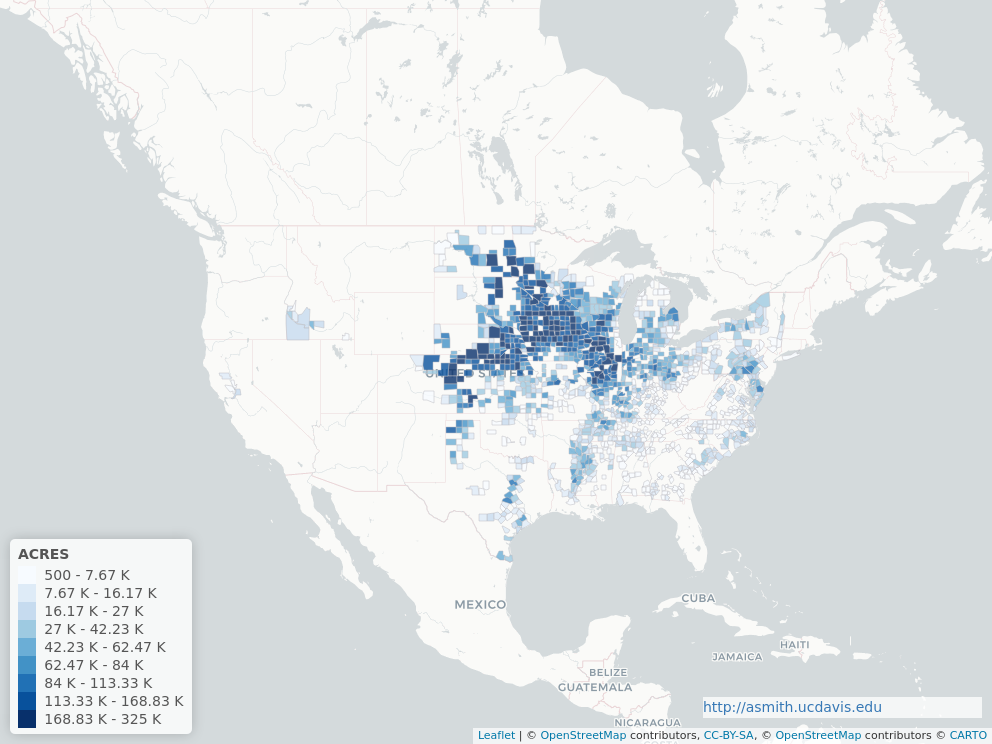
\includegraphics{assets/map_CORN_AREA PLANTED.png}

}

\caption{Corn Acres Planted 2019, map from Aaron Smith's
\href{https://asmith.ucdavis.edu/data/us-crops}{Ag Data}}

\end{figure}%

\subsection{Recent Trends in Acreage, Yields, Production, and
Use}\label{recent-trends-in-acreage-yields-production-and-use}

Corn planted acres in the U.S. has varied from just under to just over
90 million acres in recent years. Farmers in the corn belt decide how
much of their land to plant to corn and how much to plant to soybeans.
So sometimes it is said in the spring that corn and soybeans are
`competing for acres' based on the relative new crop futures prices of
corn and soybeans. If corn is more profitable, farmers will shift some
acres toward corn, and if soybeans are more profitable farmers will
shift some acres toward soybeans. Because of this, years with high corn
planted acres tend to have lower soybeans planted acres and vice versa.

Seed hybrids and genetic modification have lead to dramatic increases in
yield over the last 100 years. Although, corn planted acres have been
relatively flat for a very long time, production has skyrocketed.

The following figures
\href{http://www.ers.usda.gov/topics/crops/corn/background.aspx}{come
from} the USDA's National Agricultural Statistics Service (NASS).

\begin{figure}[H]

{\centering 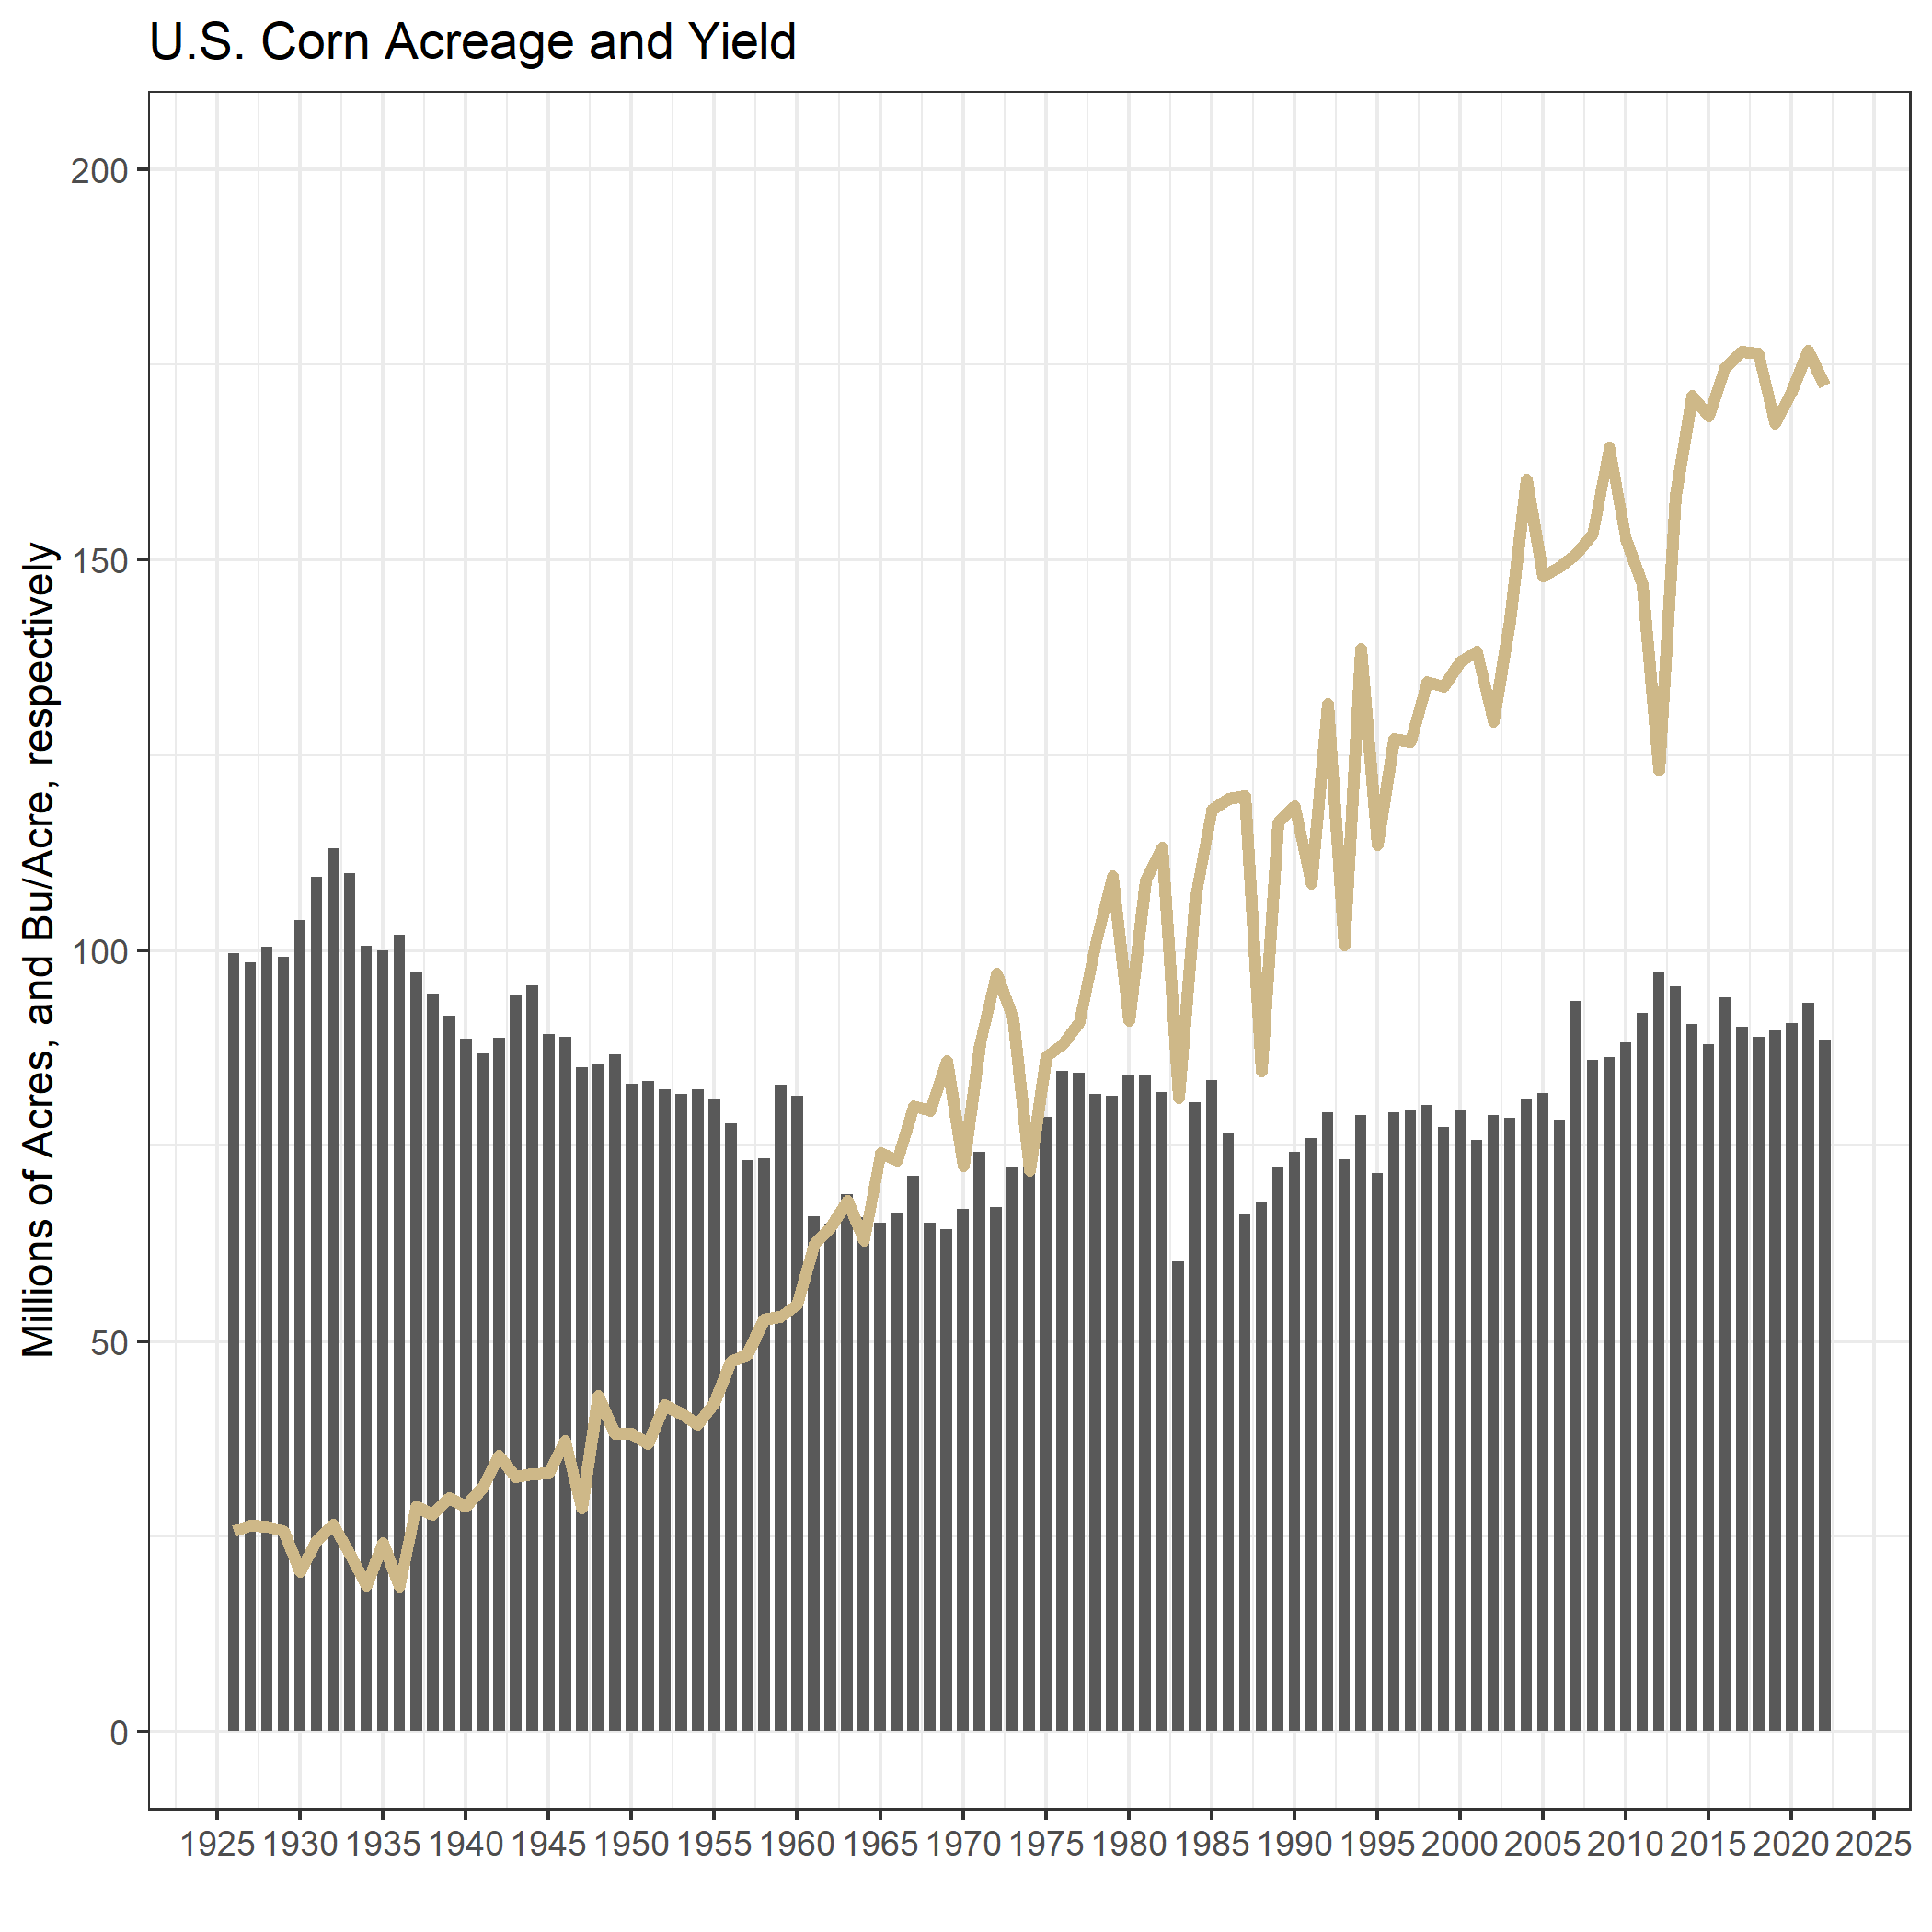
\includegraphics{assets/PrimerforGrain_CornAcandY.png}

}

\caption{Data from USDA NASS}

\end{figure}%

Corn prices can be quite volatile, with prices and production highly
inversely related to one another.

\begin{figure}[H]

{\centering 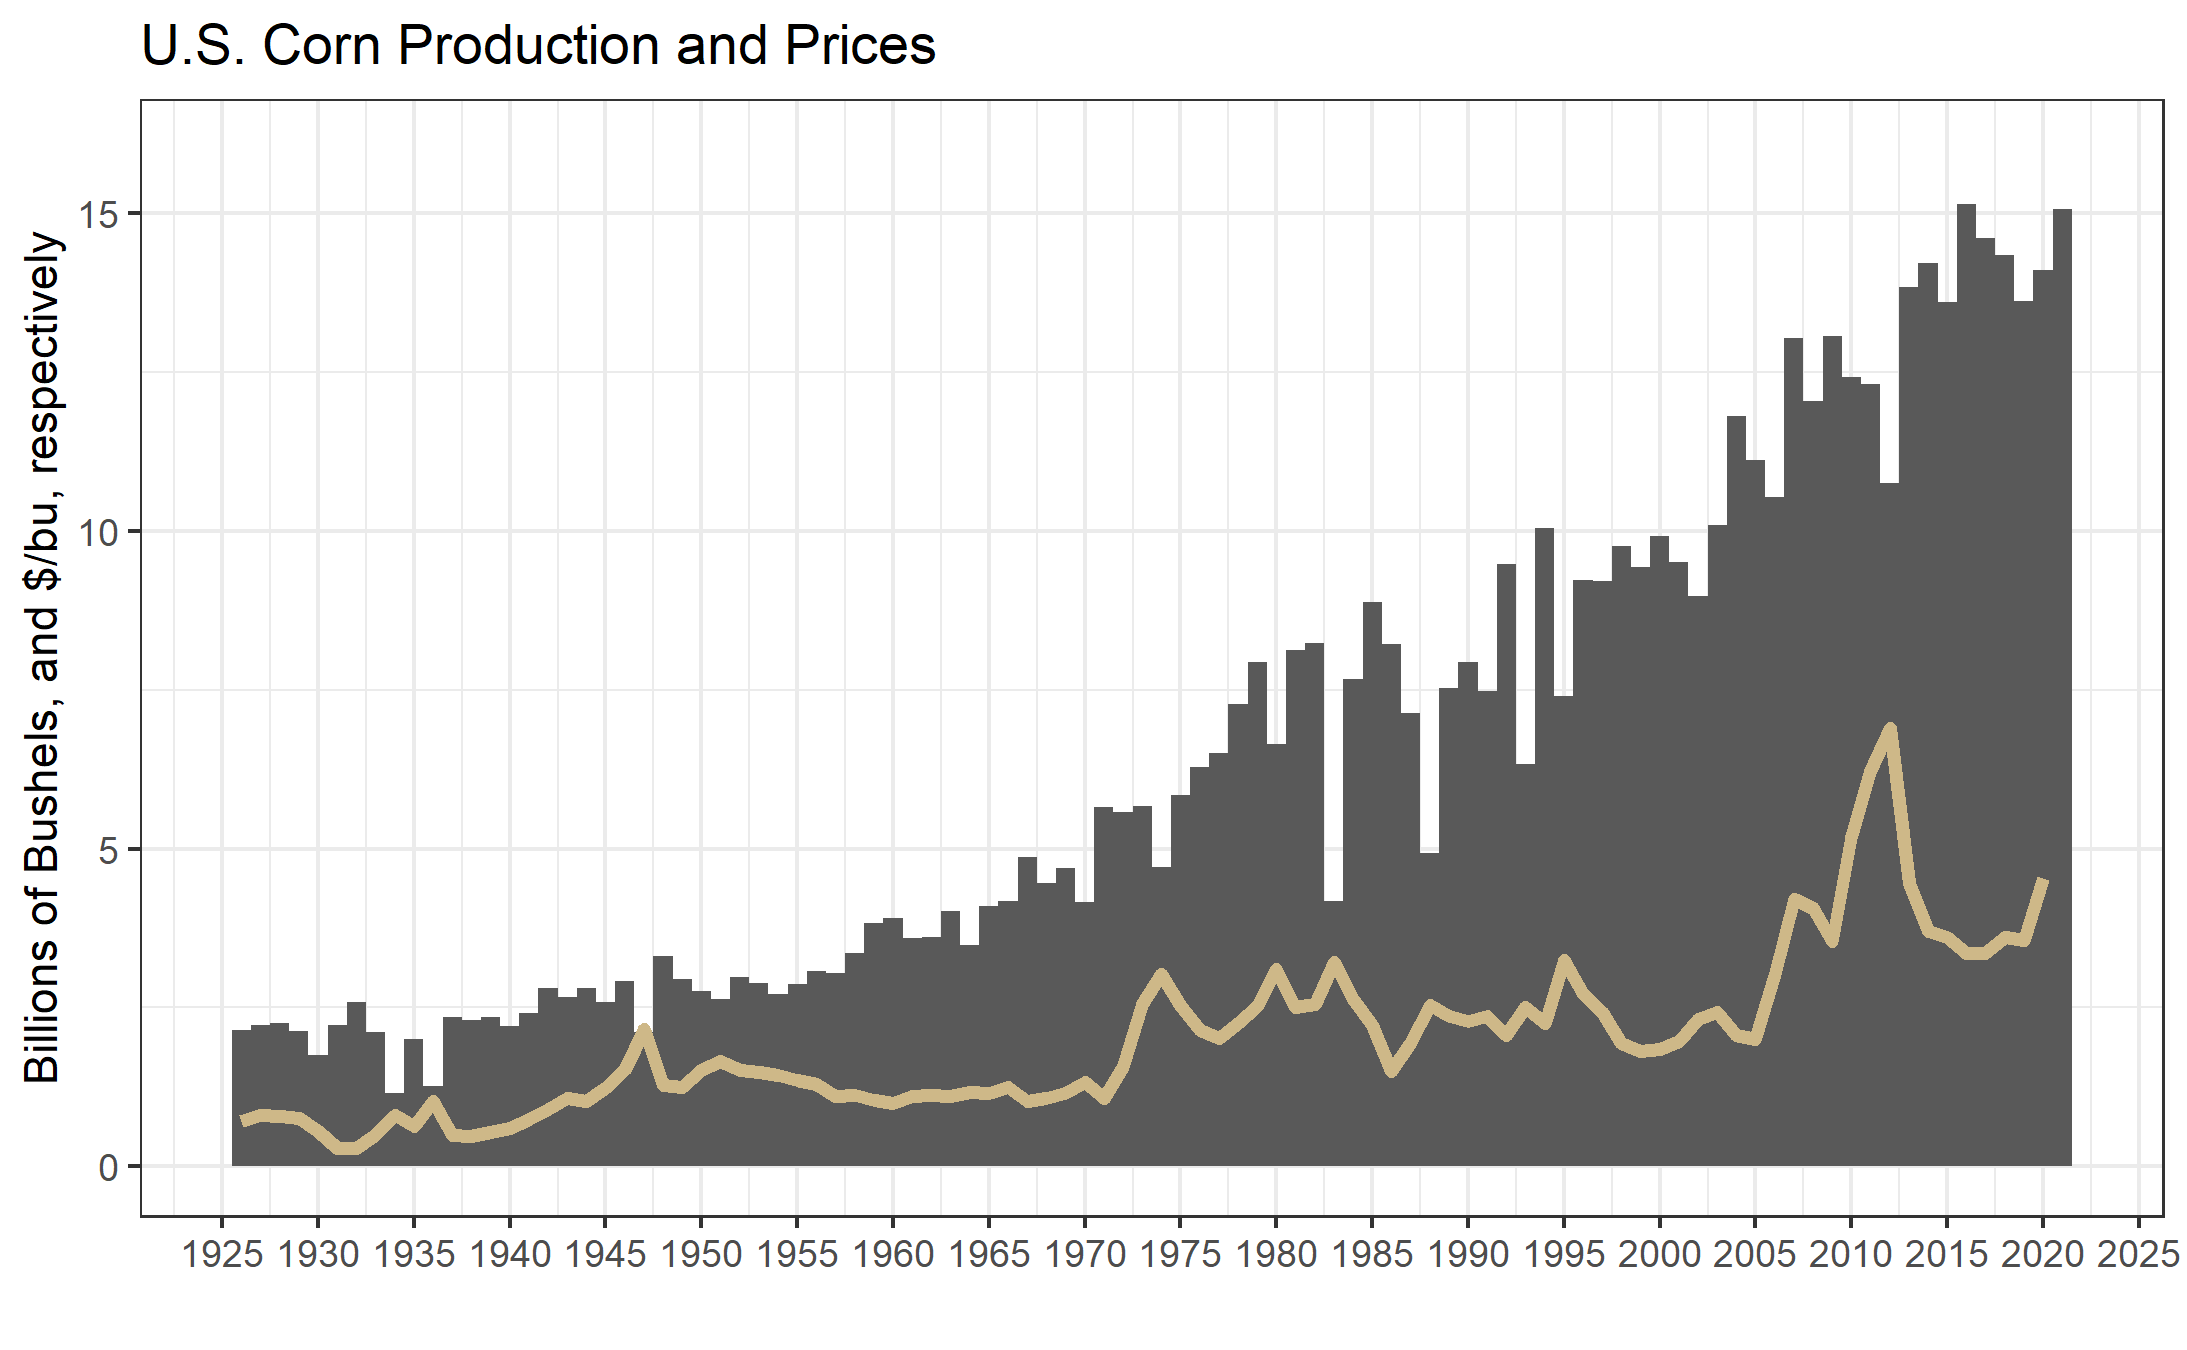
\includegraphics{assets/PrimerforGrain_CornProdand$.png}

}

\caption{Data from USDA NASS}

\end{figure}%

Corn is used in the U.S for a variety of purposes. Largest use
categories are feed (for livestock), and alcohol for fuel use (ethanol
blended with gasoline).

\begin{figure}[H]

{\centering 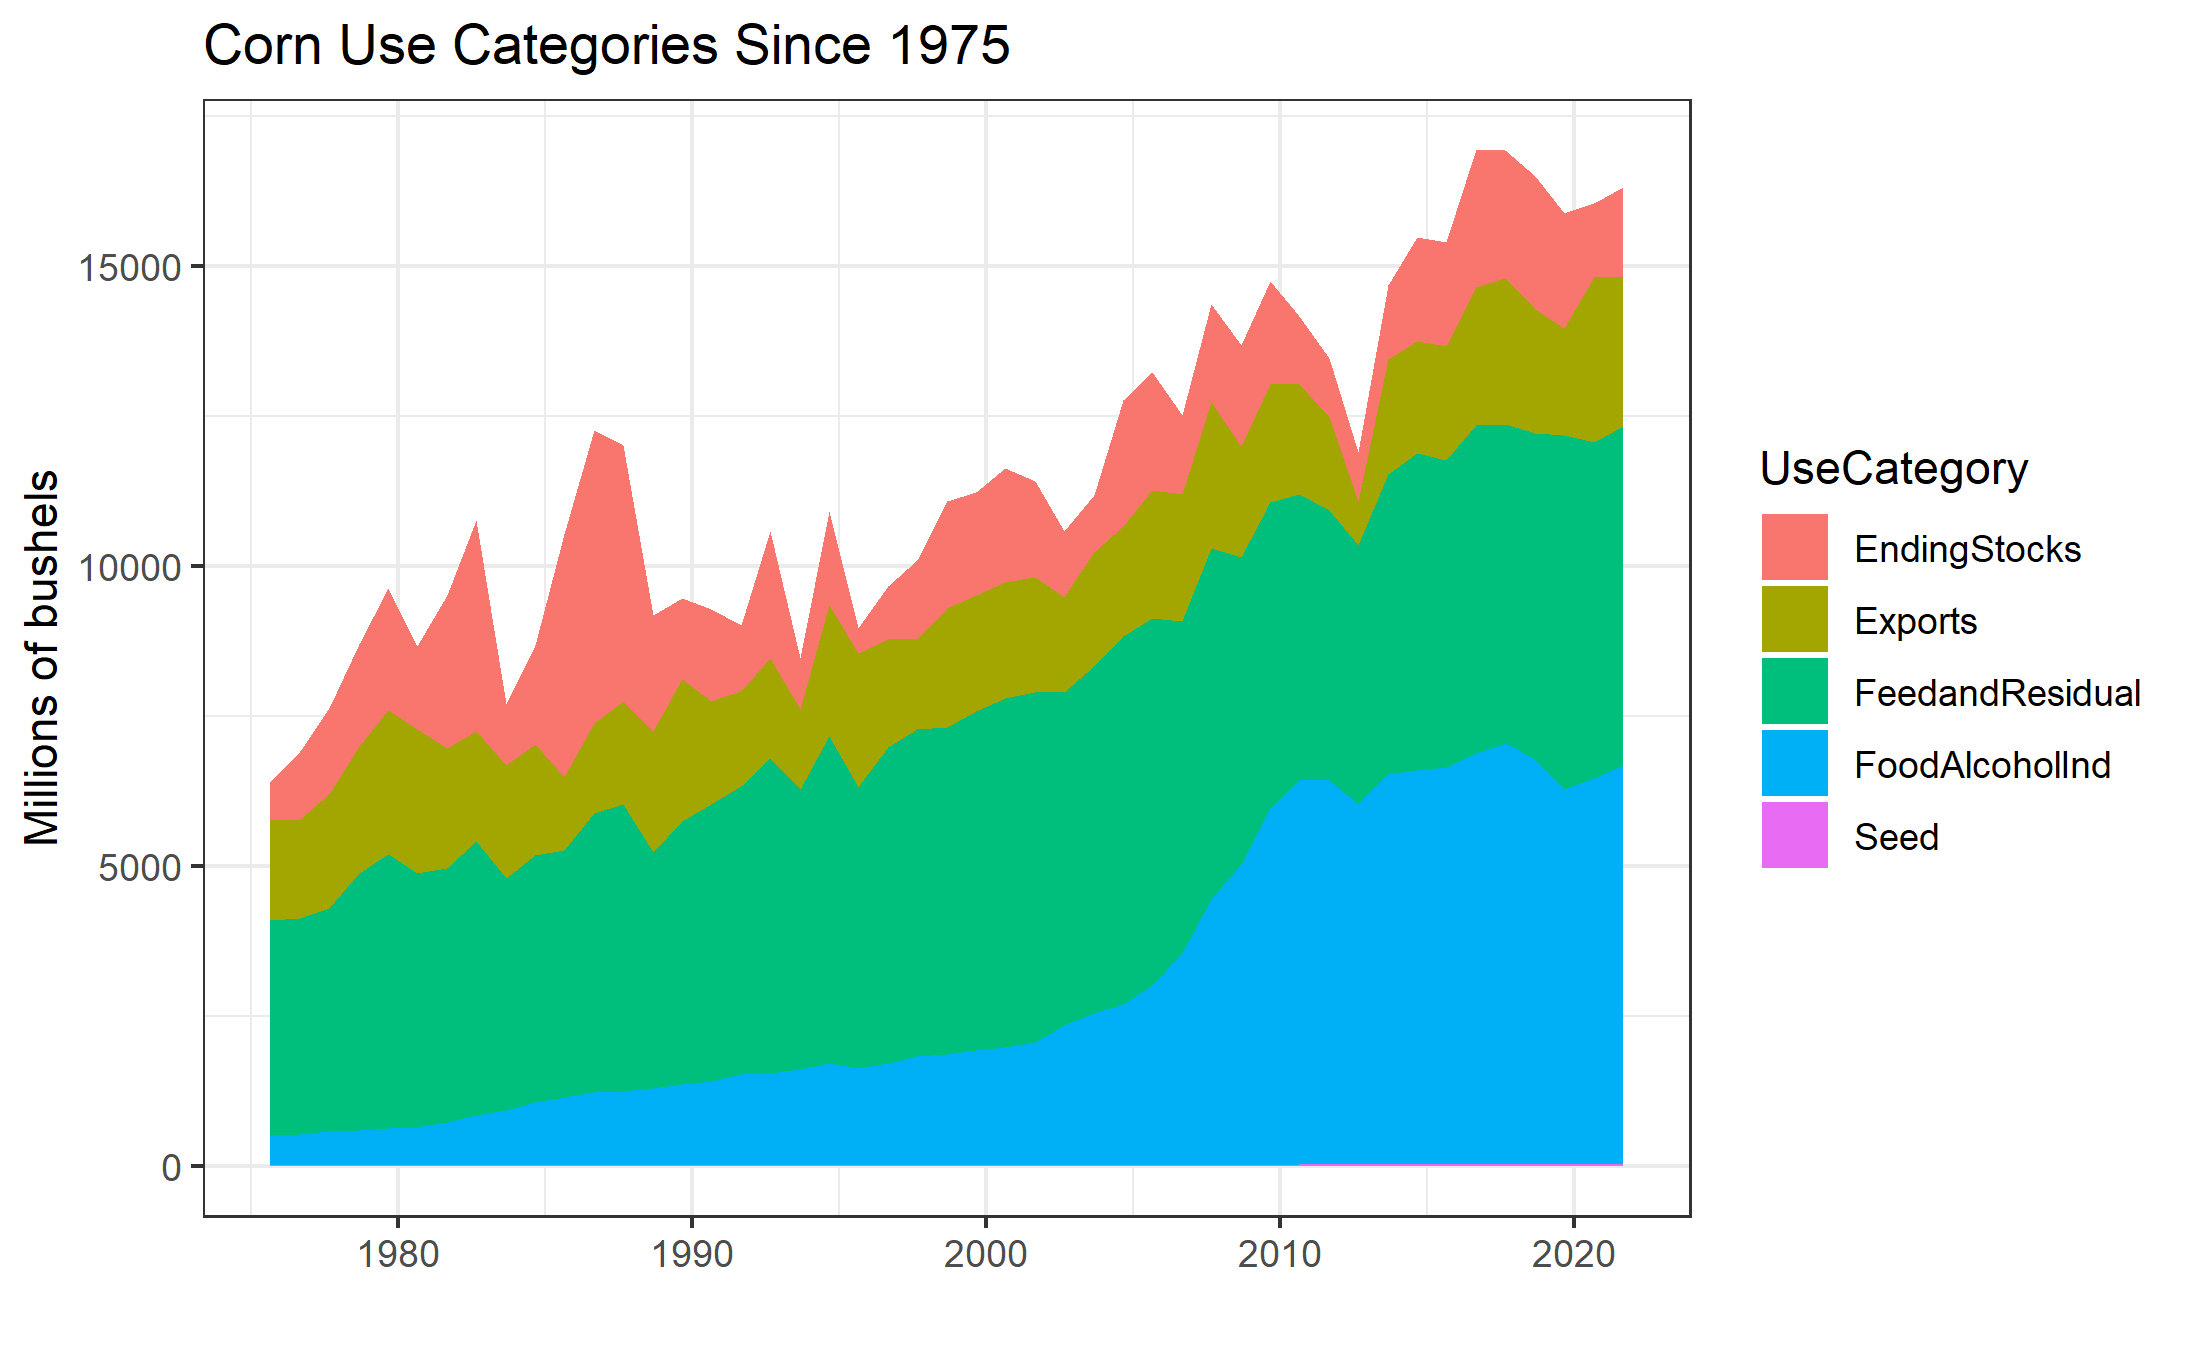
\includegraphics{assets/PrimerforGrain_CornUse.png}

}

\caption{Data from USDA ERS}

\end{figure}%

\section{Soybeans}\label{soybeans}

Soybeans are planted later than corn, from about April to June. Weather
affects soybean production prospects and generates similar price
responses as it does for corn. Soybean prices, therefore are highly
dependent on what happens during the summer months.

\begin{figure}[H]

{\centering 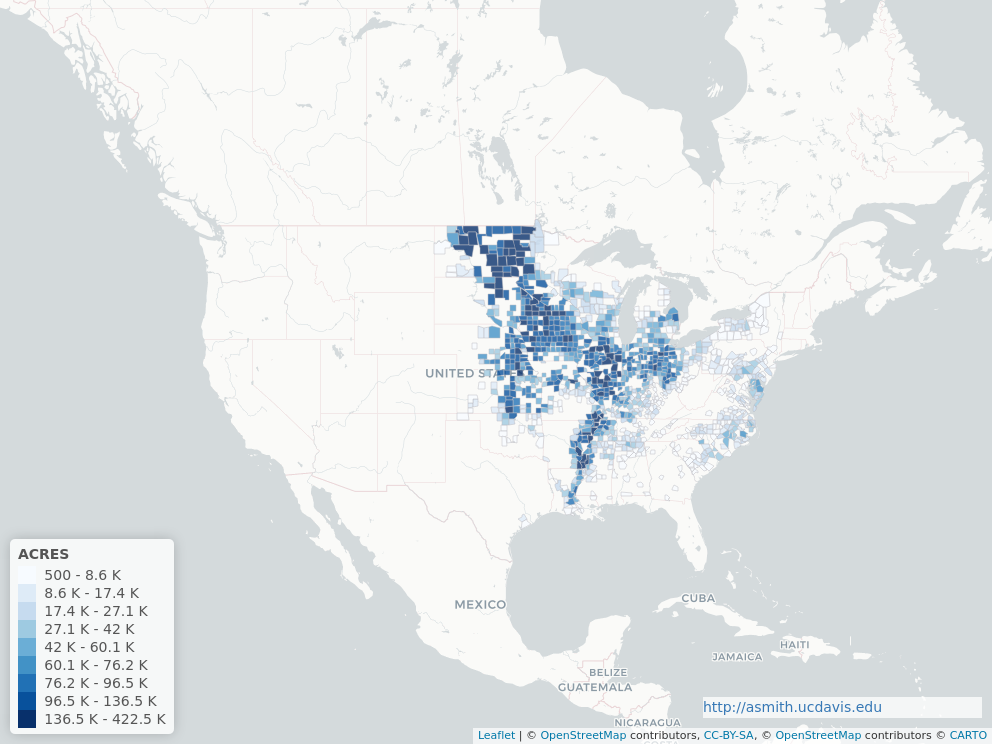
\includegraphics{assets/map_SOYBEANS_AREA PLANTED.png}

}

\caption{Soybean Acres Planted 2019, map from Aaron Smith's
\href{https://asmith.ucdavis.edu/data/us-crops}{Ag Data}}

\end{figure}%

\subsection{Recent Trends in Acreage, Yield, Production, and
Use}\label{recent-trends-in-acreage-yield-production-and-use}

Soybeans did not begin to be commercially grown in the U.S. until the

\section{Recent Trends in Acreage, Yield, Production, and
Use}\label{recent-trends-in-acreage-yield-production-and-use-1}

Soybeans were not commonly planted in the U.S. until the mid 20th
century, but once it was introduced, acreage expanded rapidly. Soybeans
have also benefited from improved yields due to biotechnology.

\begin{figure}[H]

{\centering 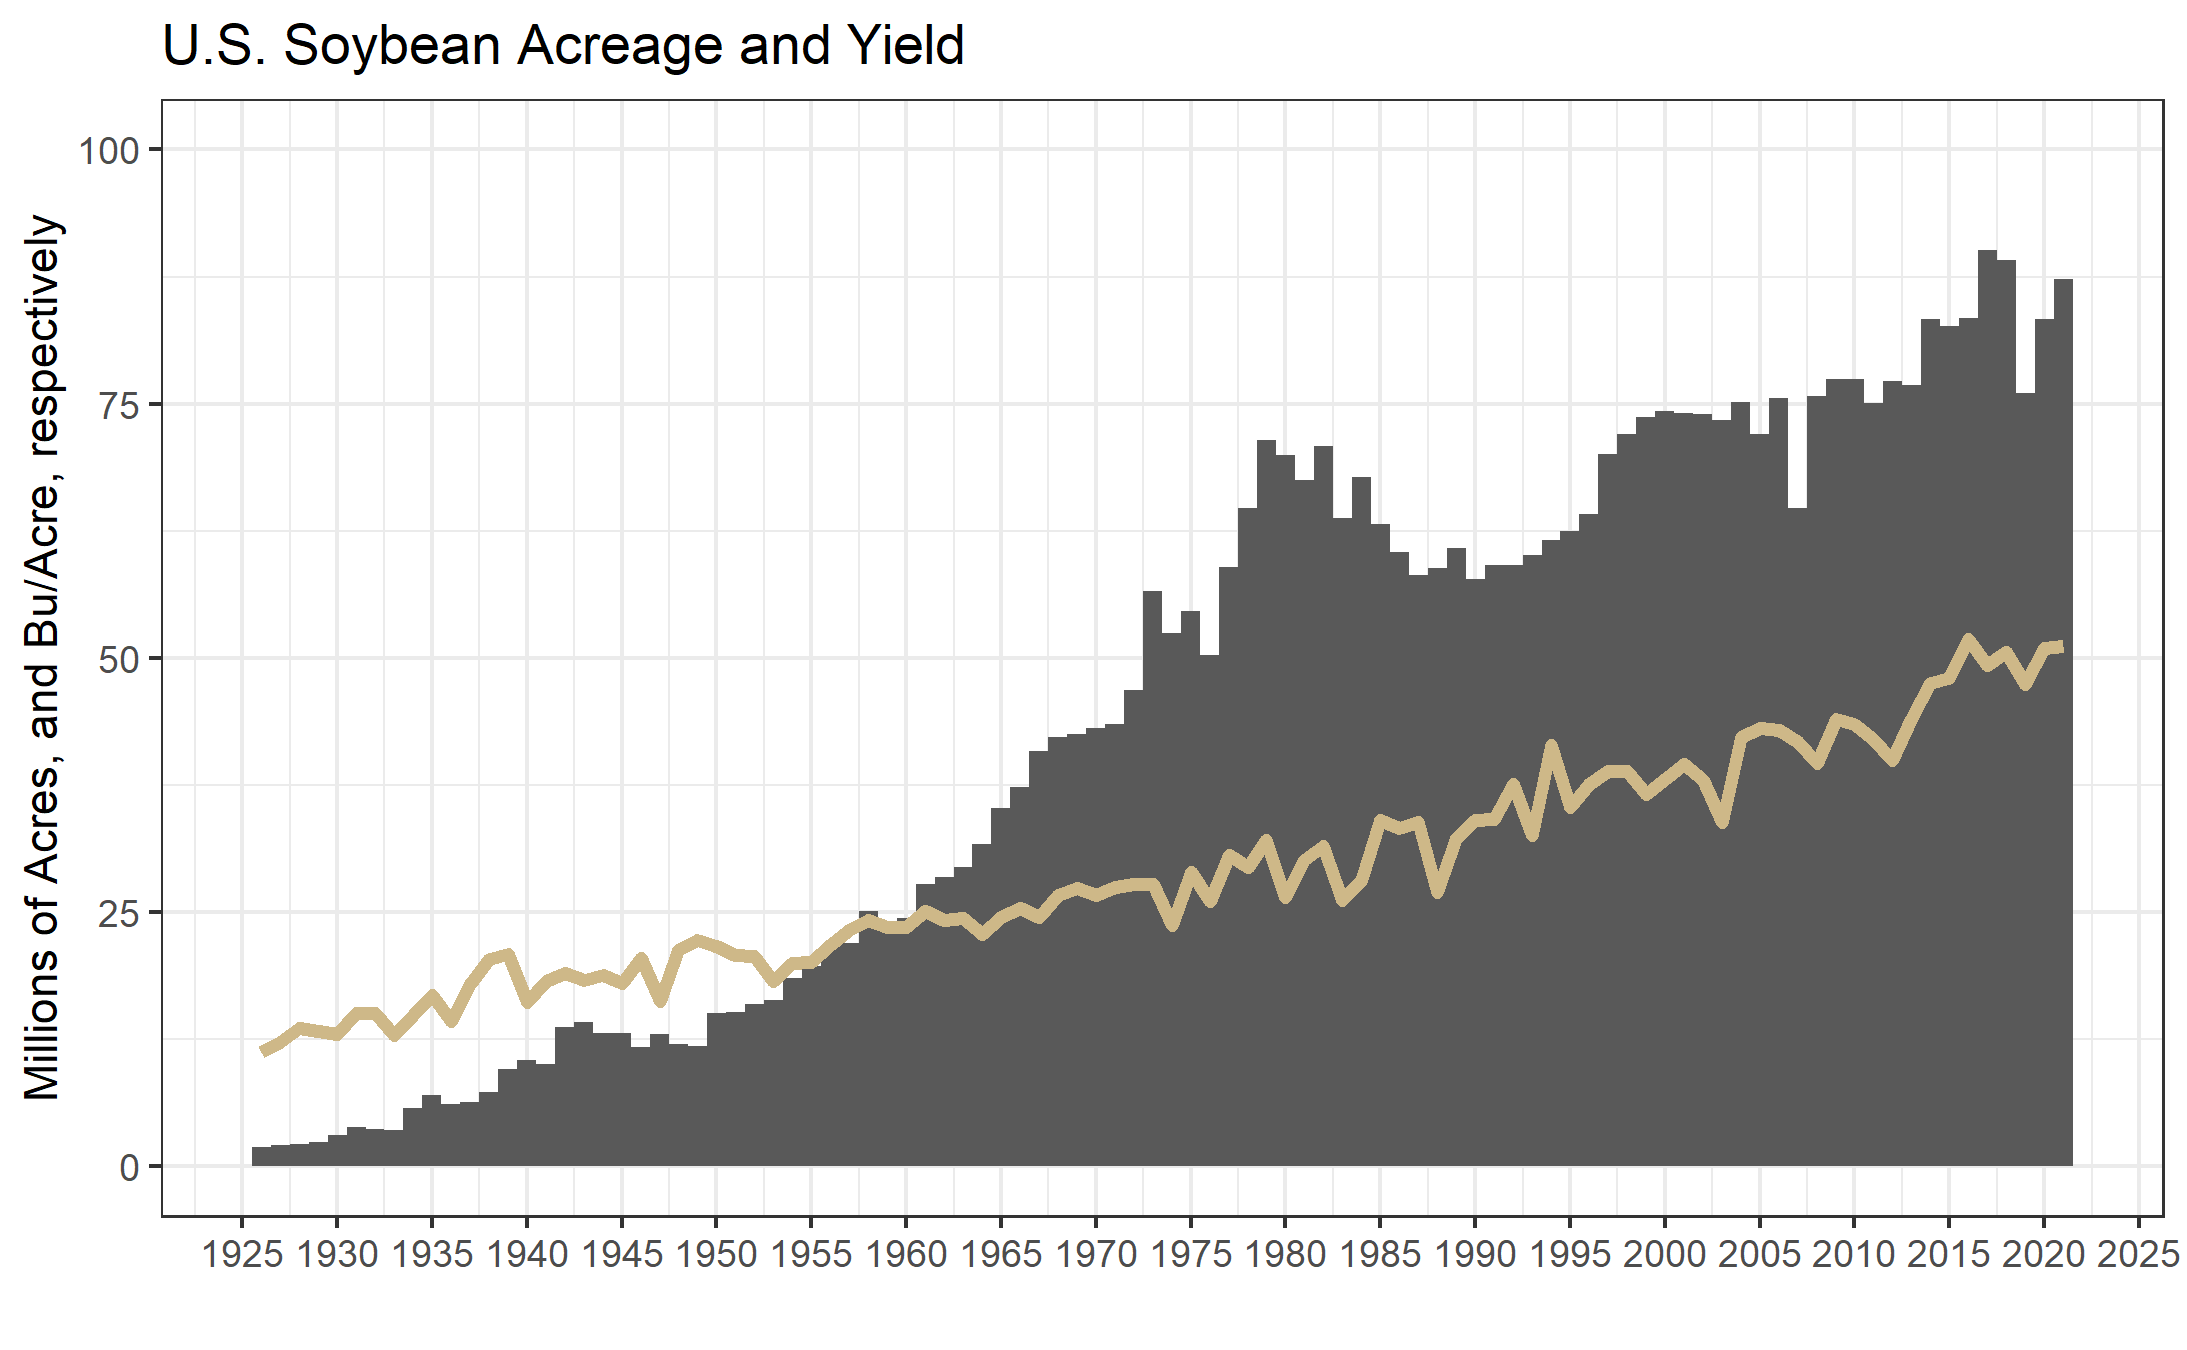
\includegraphics{assets/PrimerforGrain_SoyAcandY.png}

}

\caption{Soybean Acres and Yield}

\end{figure}%%
\begin{figure}[H]

{\centering 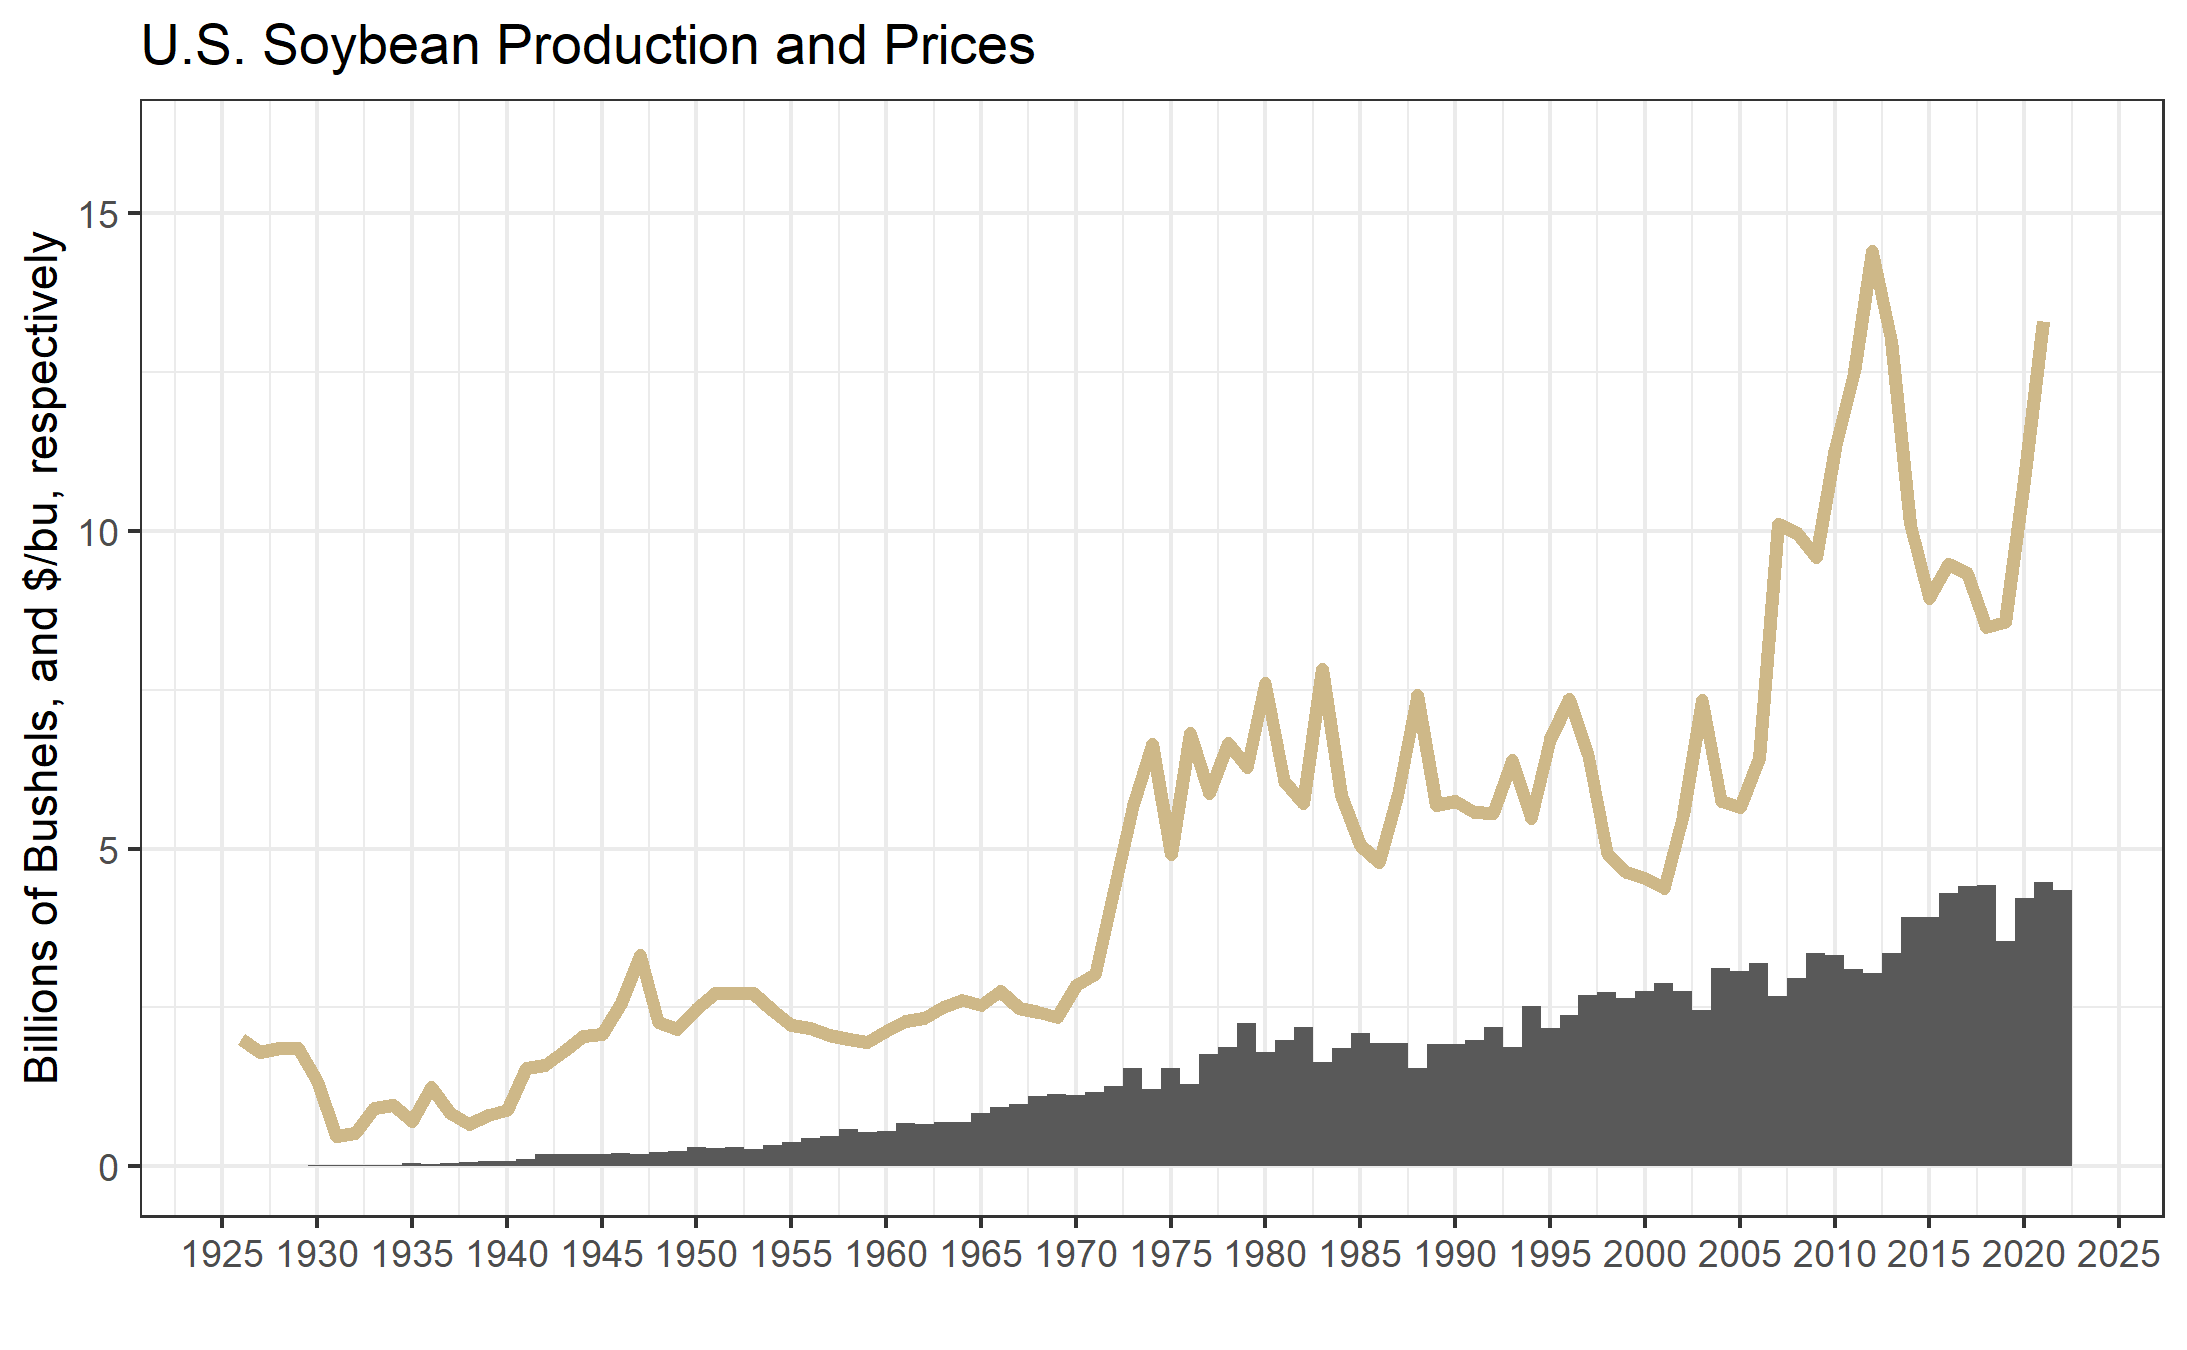
\includegraphics{assets/PrimerforGrain_SoyProdand$.png}

}

\caption{Soybean Production and Prices, Data from USDA NASS}

\end{figure}%

Soybeans consumed in the U.S. are almost exclusively processed into
soybean meal and soybean oil, a process referred to as `crushing'.
Soybean meal is high in protein and used as an ingredient in livestock
feed. Soybean oil is used for a variety of things, but the bulk of it is
consumed as edible oil.

About half of the soybeans produced in the U.S. are exported, and more
than half of soybeans exported are
\href{http://farmdocdaily.illinois.edu/2015/03/footprint-of-chinese-demand-for-us-soybeans.html}{imported
by China}.

\begin{figure}[H]

{\centering 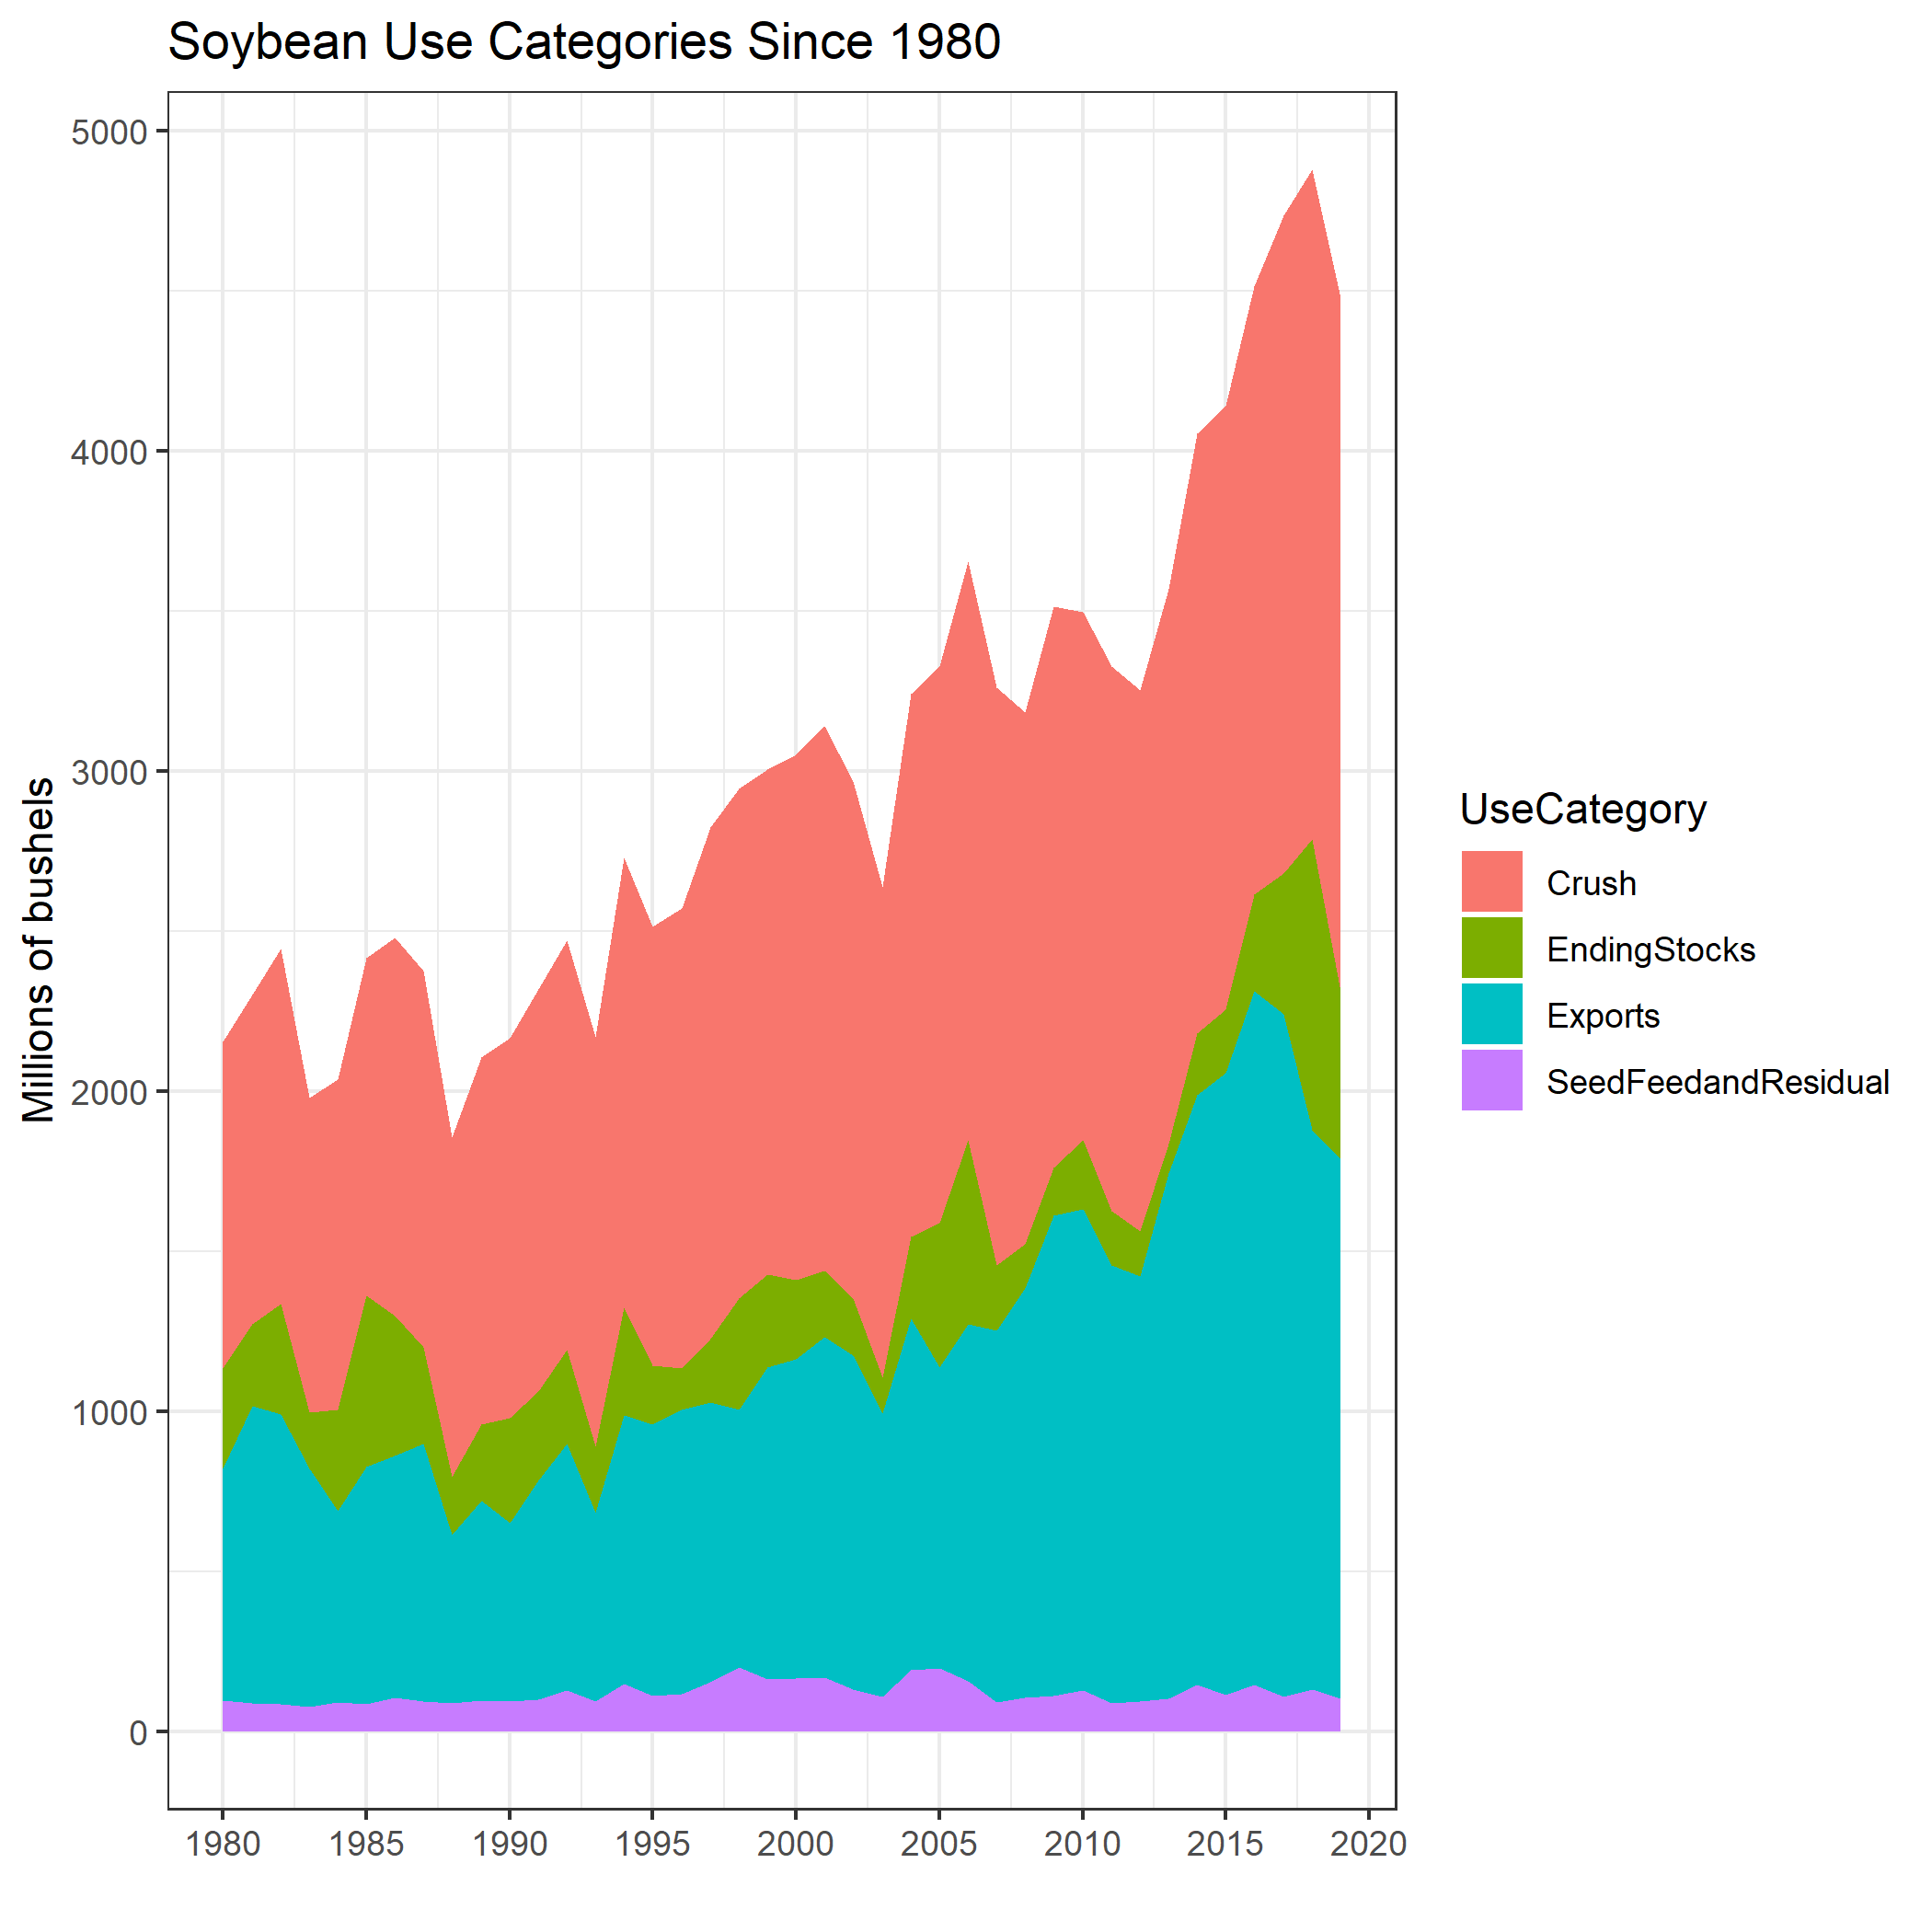
\includegraphics{assets/PrimerforGrain_SoyUse.png}

}

\caption{Data from USDA ERS}

\end{figure}%

\section{Wheat}\label{wheat}

There are three main types of wheat grown in the U.S. Hard Red Winter
Wheat (HRW/KC Wheat), Hard Red Spring Wheat (HRS/Minneapolis wheat), and
Soft Red Winter Wheat (SRW/Chicago Wheat). Each of these types of wheat
have its own futures contract, are grown in distinct regions of the
country, and have different end uses. The main distinction between the
types of wheat is how much protein is contained in the kernels. This
variation in protein also determines what the variety of wheat is
ultimately used for.

\begin{figure}[H]

{\centering 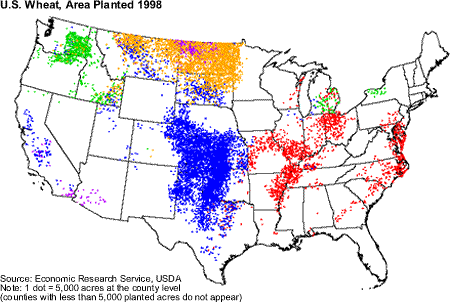
\includegraphics{images/Wheat-Growing-Areas.png}

}

\caption{Figure 8: Wheat Variety Growing Areas}

\end{figure}%

(Source
\href{https://wayback.archive-it.org/5923/20120310141642/http://ers.usda.gov/Briefing/Wheat/maps.htm}{USDA-ERS})

Blue = HRW\\
Gold = HRS\\
Red = SRW

\subsection{Hard Red Winter Wheat}\label{hard-red-winter-wheat}

HRW wheat is planted in the fall and lays dormant or grows very little
during the winter. As temperatures rise in the spring, wheat plants
start to grow. It looks like grass before it is mature. During April and
May the wheat plants make `heads' where the wheat kernels grow. When the
plants die the grain is harvested.

HRW wheat is primarily used to make bread flour.

Hard Red Winter Wheat is sometimes called Kansas City Wheat because the
Kansas City Board of Trade had a HRW wheat futures contract. The KCBOT
was recently bought by the CME Group, but HRW continues to be known as
KC wheat.

\begin{figure}[H]

{\centering 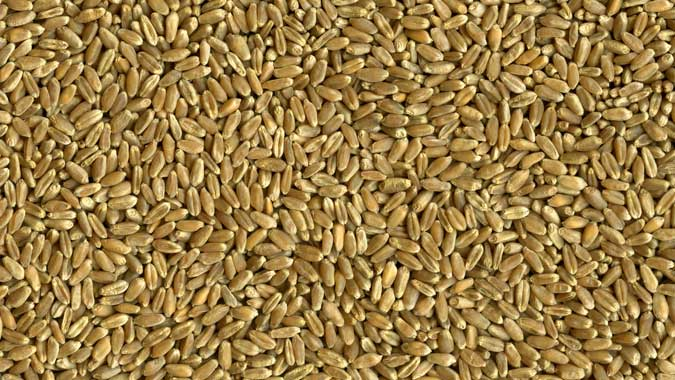
\includegraphics{images/HRW-Wheat.jpg}

}

\caption{Figure 9: Hard Red Winter Wheat}

\end{figure}%

(Source
\href{https://www.gipsa.usda.gov/fgis/commgallery/gr_hrw.aspx}{USDA-GIPSA})

\subsection{Hard Red Spring Wheat}\label{hard-red-spring-wheat}

Hard red spring wheat is planted in the spring, around April or May and
is harvested in the fall, around September. It has the highest protein
content (13-16\%) of all the major wheat varieties, making it high in
gluten content, which is good for baking bread. It also is used to blend
with lower protein wheat flour varieties to increase the protein
content.

HRS wheat is referred to as Minneapolis Wheat because the
\href{http://www.mgex.com/}{Minneapolis Grain Exchange} offers a futures
contract in HRS wheat.

\begin{figure}[H]

{\centering 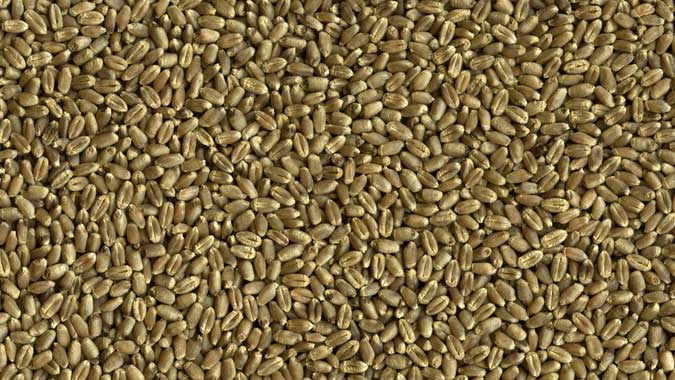
\includegraphics{images/HRS-Wheat.jpg}

}

\caption{Figure 10: Hard Red Spring Wheat}

\end{figure}%

(Source
\href{https://www.gipsa.usda.gov/fgis/commgallery/gr_hrs.aspx}{USDA-GIPSA})

\subsection{Soft Red Winter Wheat}\label{soft-red-winter-wheat}

Soft Red Winter Wheat is planted in the fall, and is harvested in the
late spring, like HRW wheat. Soft red winter wheat is lower in protein
which makes is suitable for use in cakes, cookies, and crackers, where
high gluten content is not required.

SRW wheat is referred to as Chicago Wheat because the Chicago Board of
Trade offers a futures contract for SRW wheat.

\begin{figure}[H]

{\centering 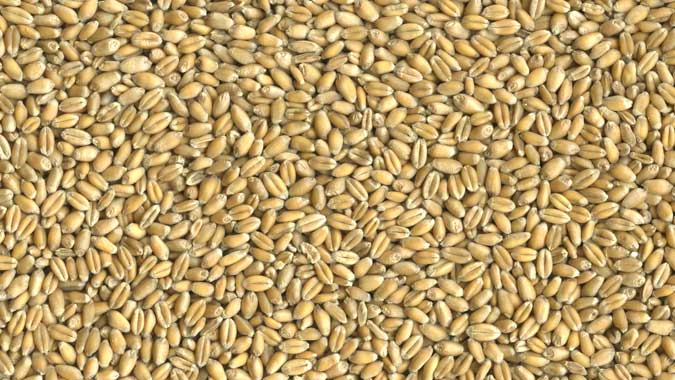
\includegraphics{images/SRW-Wheat.jpg}

}

\caption{Figure 11: Soft Red Winter Wheat}

\end{figure}%

(Source
\href{https://www.gipsa.usda.gov/fgis/commgallery/gr_srw.aspx}{USDA-GIPSA})

\subsection{Protein Premiums and Wheat
Spreads}\label{protein-premiums-and-wheat-spreads}

If you follow wheat markets for long, you will hear discussion of
`protein premiums', that is because flour millers rarely use just one
kind of wheat to make their flour. They blend different types of wheat
together to make flours of varying protein and gluten levels.

Different varieties of wheat naturally have different protein levels, as
mentioned above. However, there is also a link between yield and protein
levels. When yields are high, wheat protein is lower. This means during
years where lower protein winter wheat has good yields, there is plenty
of wheat, but not necessarily enough protein. This causes the price of
higher protein wheat, like spring wheat, to rise against the price of
winter wheat. If winter wheat crops are smaller around the world, the
protein content is higher, and spring wheat may not enjoy a large
premium against winter wheat.

Because of this dynamic, the relative prices of Minneapolis, Kansas
City, and Chicago wheat futures are closely followed by stakeholders in
any of the wheat markets.

\section{Recent Trends in Acreage, Yield, Production, and
Use}\label{recent-trends-in-acreage-yield-production-and-use-2}

\begin{figure}[H]

{\centering 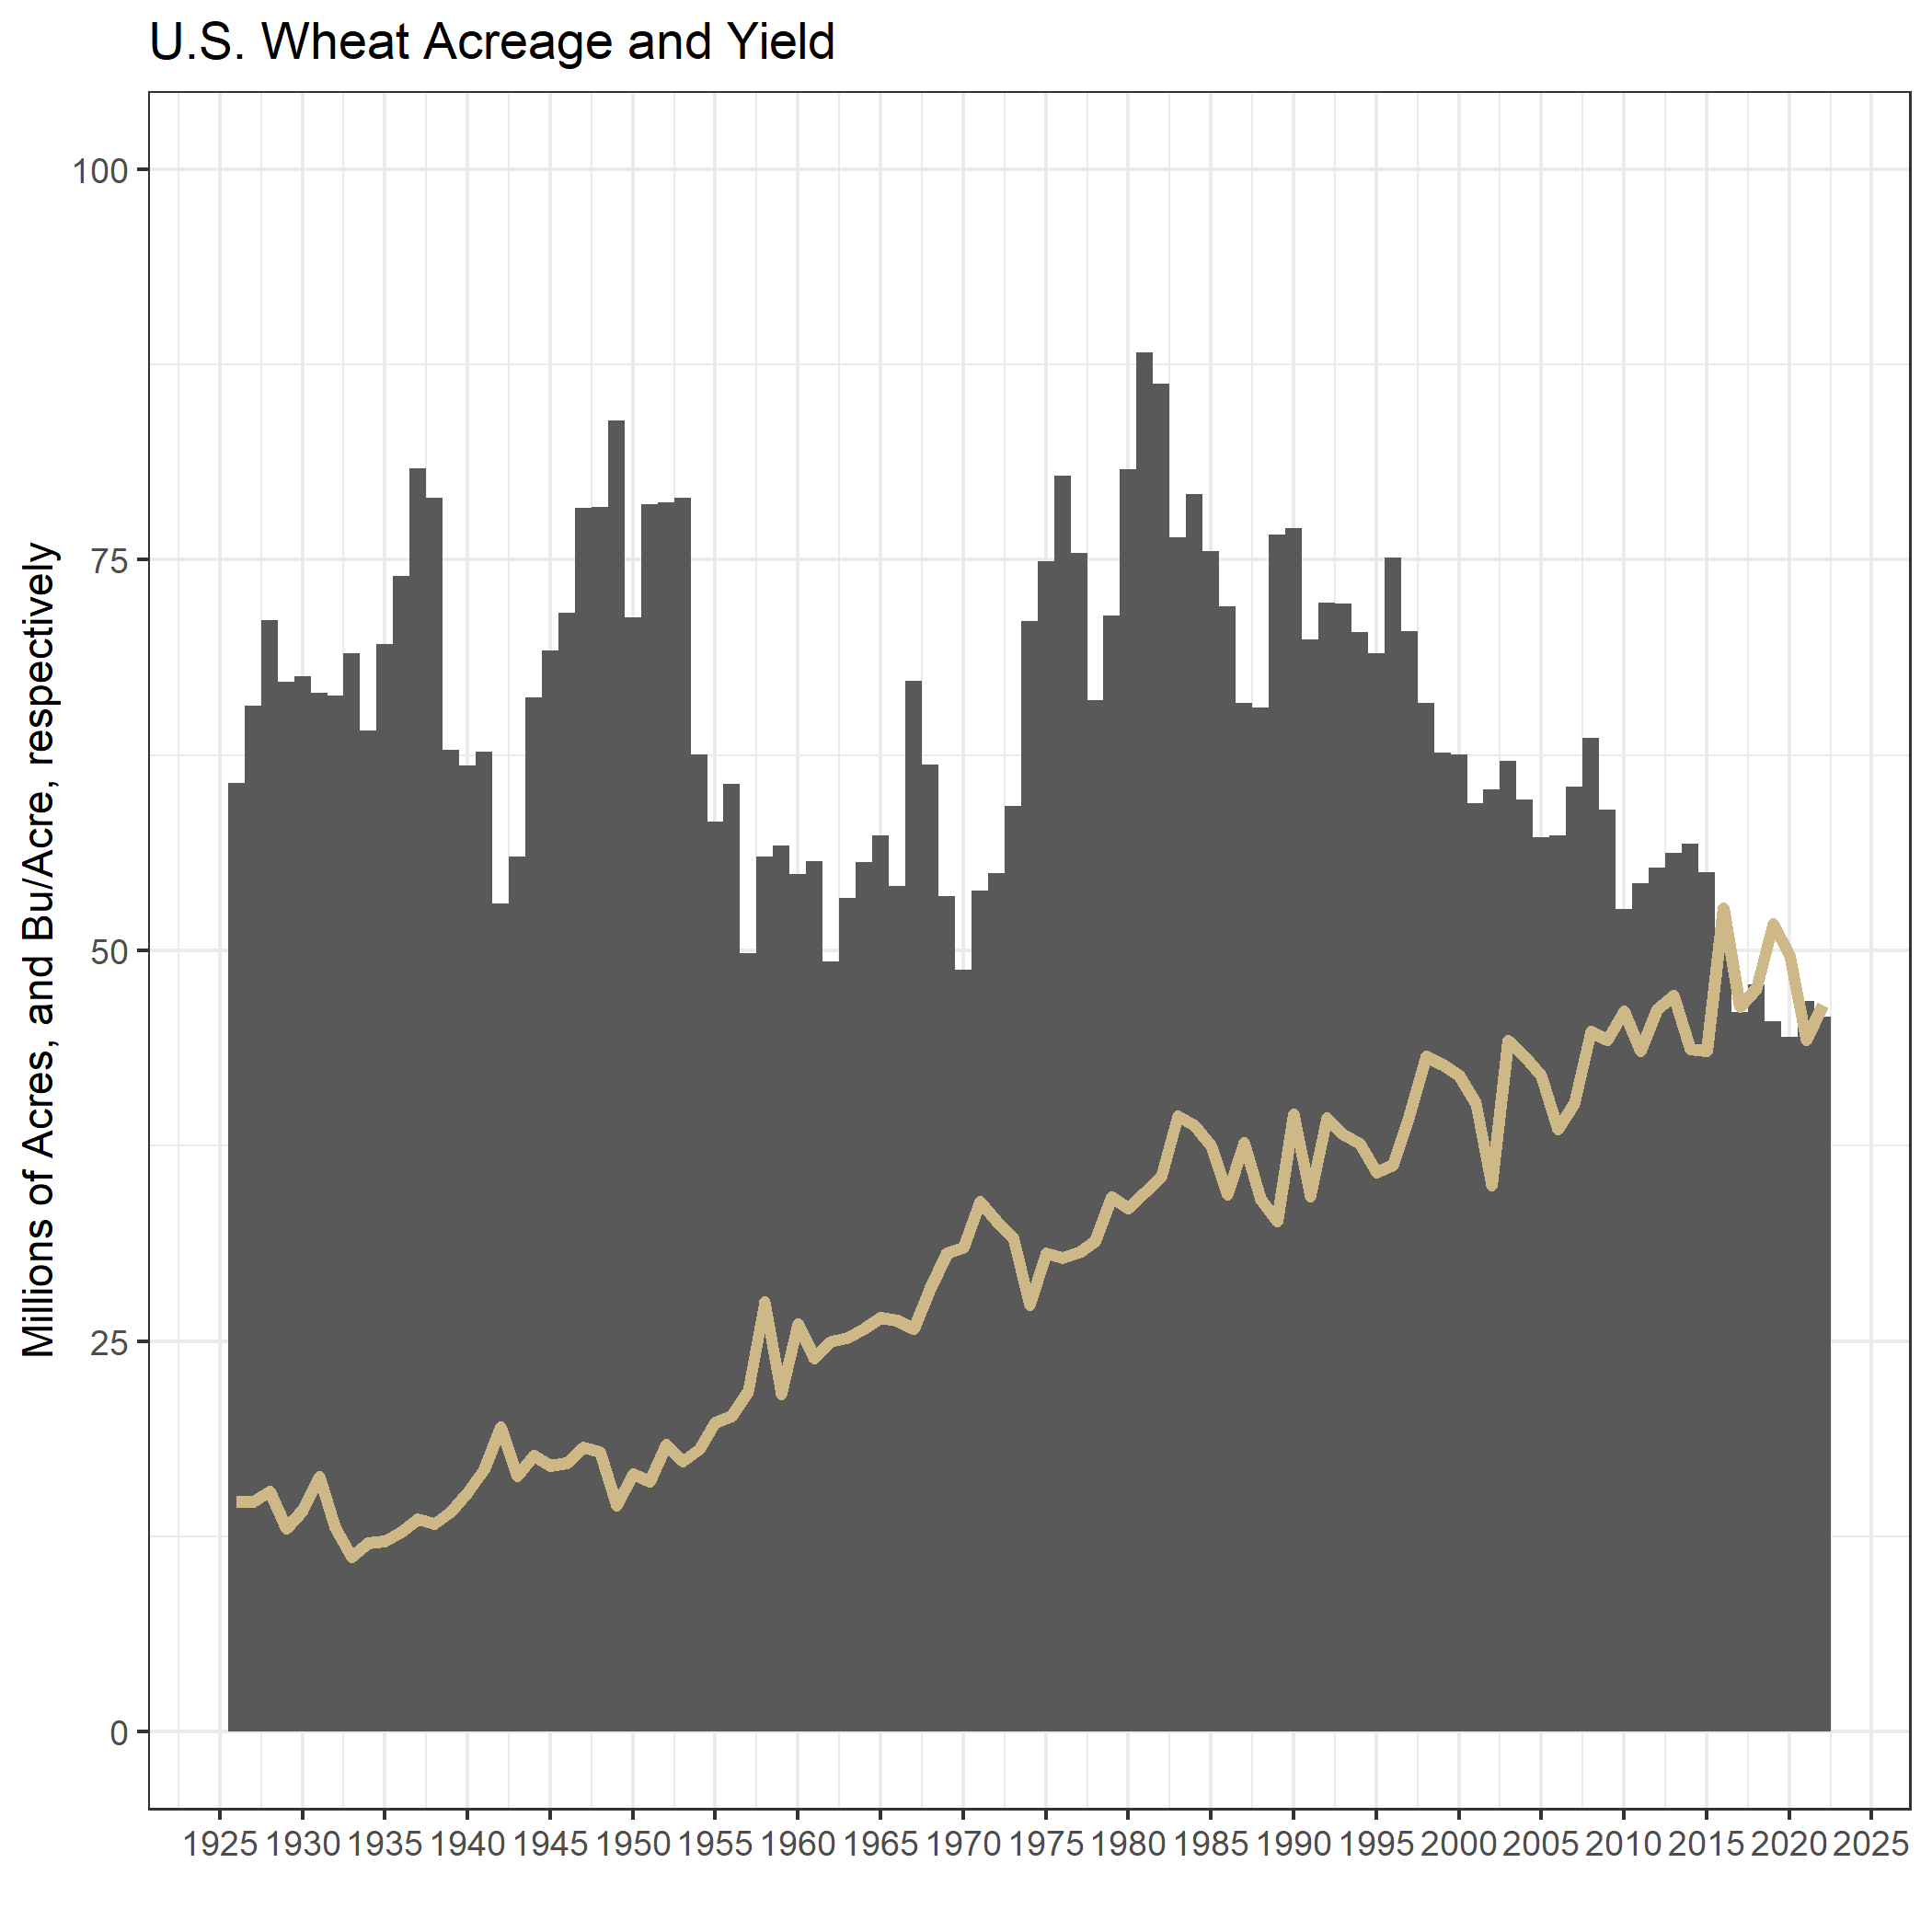
\includegraphics{assets/PrimerforGrain_WheatAcandY.png}

}

\caption{Data from USDA NASS}

\end{figure}%%
\begin{figure}[H]

{\centering 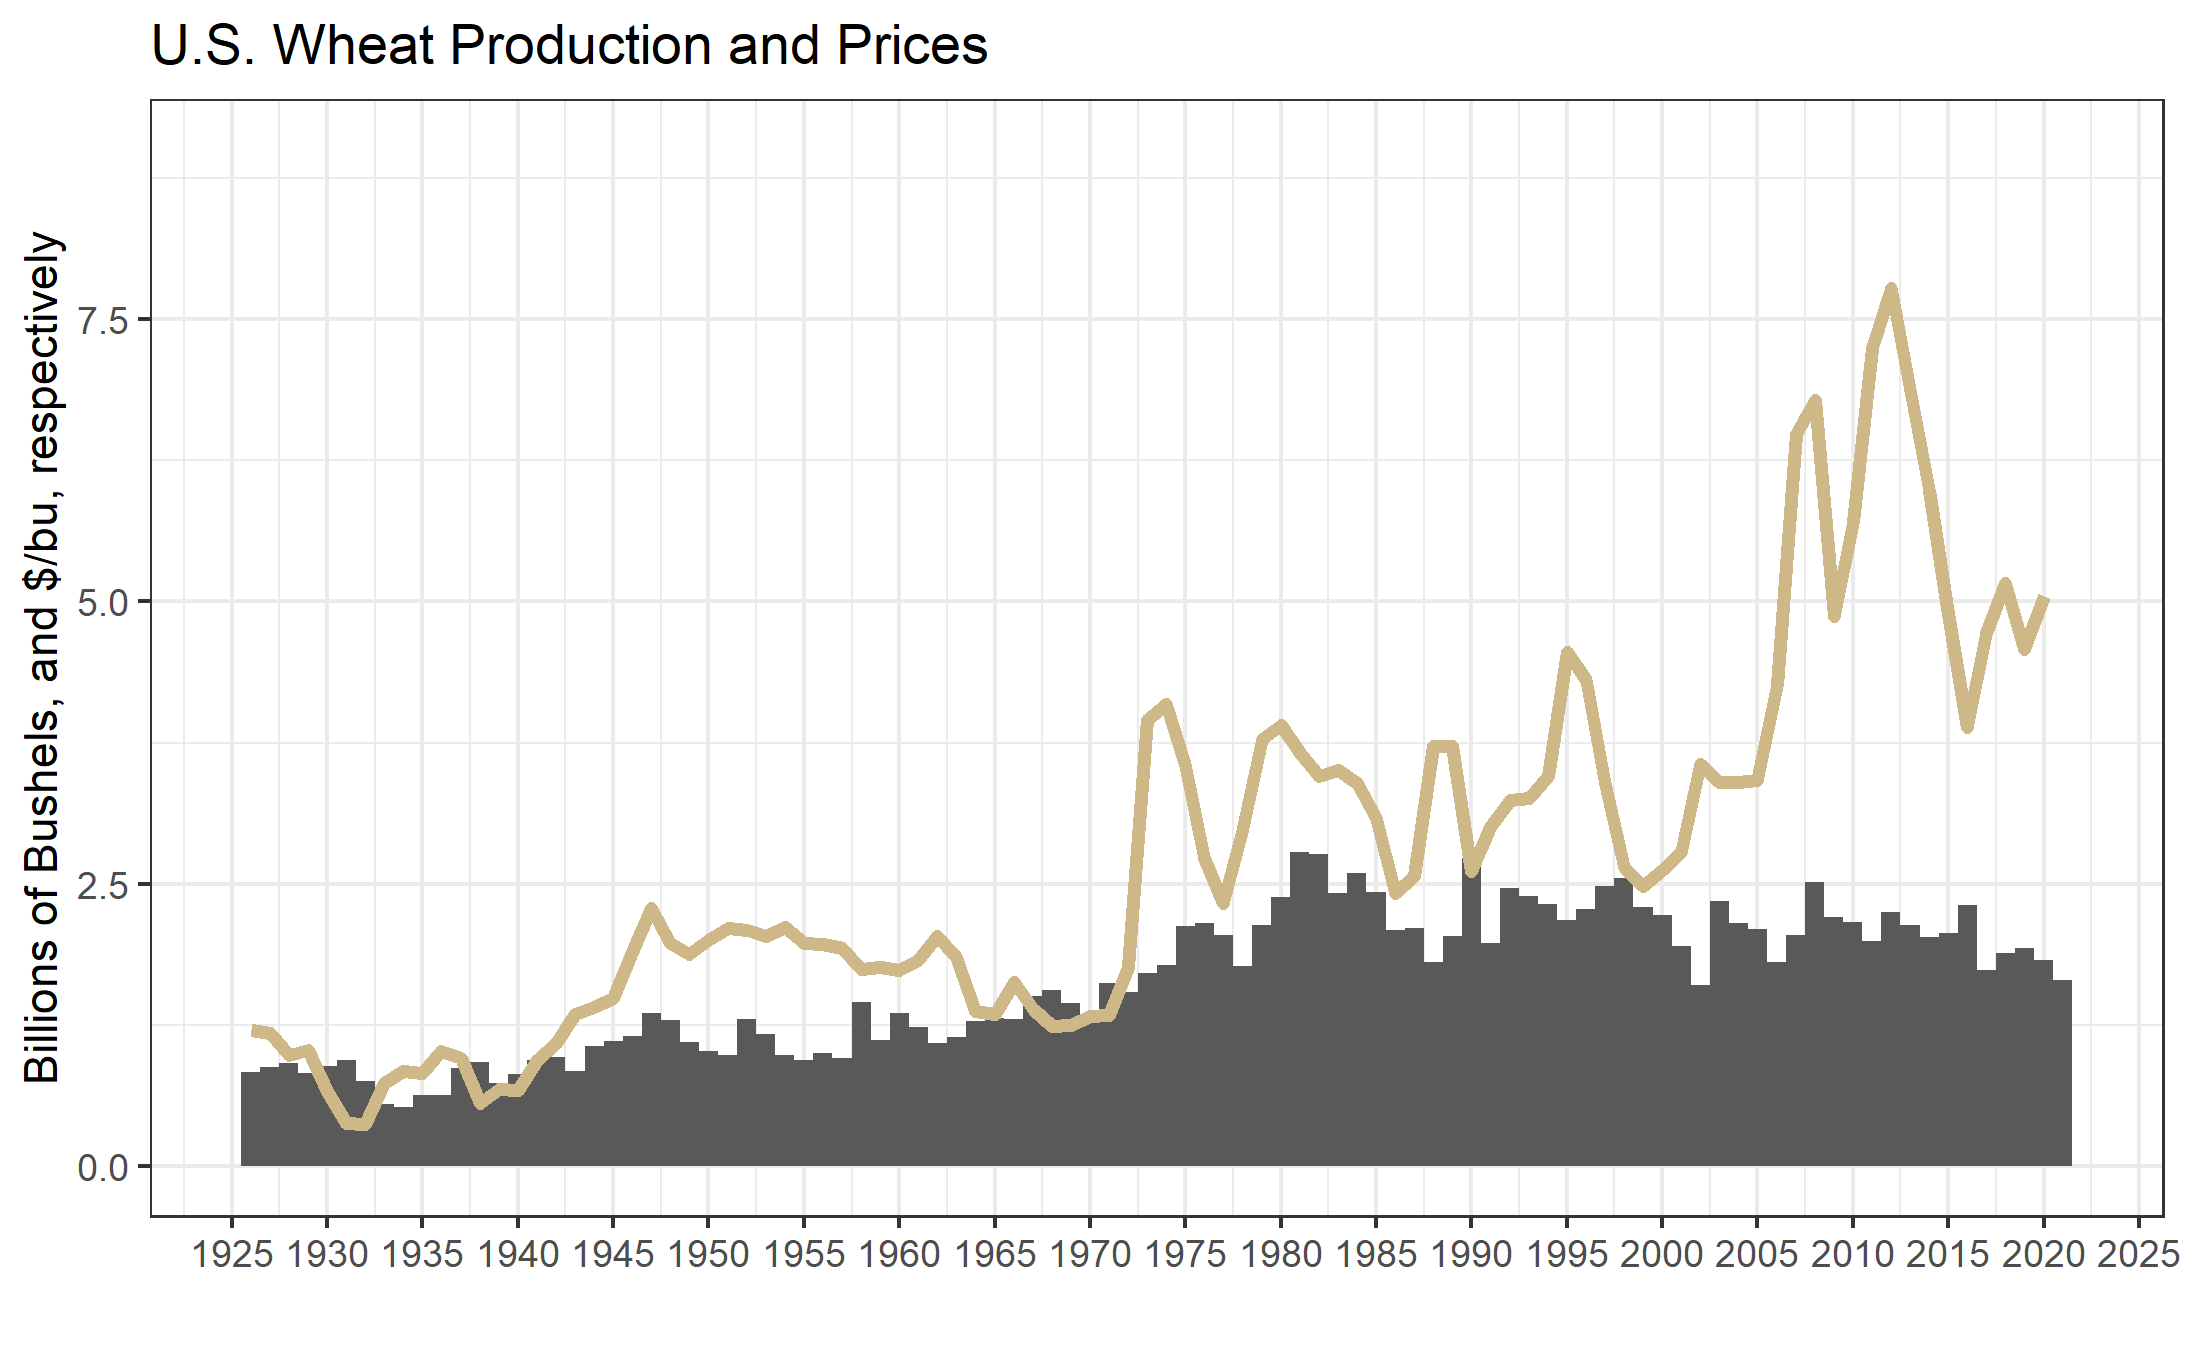
\includegraphics{assets/PrimerforGrain_WheatProdand$.png}

}

\caption{Data from USDA NASS}

\end{figure}%

\bookmarksetup{startatroot}

\chapter{Commodity Price Analysis and
Forecasting}\label{commodity-price-analysis-and-forecasting}

{Interested in more? Please let me know by}
\href{https://forms.gle/Q3VByCQZHjfQSy9D7}{taking the survey}!

A commodity is a good that can be supplied without qualitative
differences. A bushel of wheat is regarded as a bushel of wheat
everywhere. Commodities are fully or partially fungible so that the
market treats a unit of good the same no matter who produced it or where
it was produced. Think of grain elevators, for example. Farmers bring
their grain to an elevator at harvest. Sometimes they sell it outright
to the elevator, but sometimes they pay the elevator to store it for
them. When the farmer decides to come get his grain out of storage do
you think he gets the exact same kernels he brought in? Of course that
would be impractical. The elevator just gives him back the same amount
of grain he brought in of the same quality. The farmer is happy because
the wheat is fungible. The grain he will be able to sell the grain he
took out just as easily as the grain he put in. This is in stark
contrast to differentiated goods where branding and quality make
important distinctions between goods, resulting in differentiated
demands. Just try to find someone indifferent between iPhone and
Android!

Since commodities are fungible, it also makes sense that prices of
commodities are determined by the entire (often global) market for the
good. They tend to be basic resources such as agricultural and food
products, metals, energy, an fibers. The fungibility of commodities
enables the commodity to be traded in centralized spot and futures
markets.

\subsection{Trasformation Over Space, Time, and
Form}\label{trasformation-over-space-time-and-form}

Commodities can undergo various transformations. Standard price analysis
usually groups these into three broad categories: Space, Time, and Form.
Studying a commodity's transformation over space comes about from the
fact that the production of a commodity is often concentrated in a
specific geographic location, while consumption of commodities is
usually dispersed. In order for traders to have incentive to move a
commodity from one location to another, a certain patter of prices must
prevail. In short, traders must be able to make a profit, or at least
break even in the business of moving a commodity from one location to
another.

Studying a commodity's transformation through time considers the nature
of prices required to provide incentive to store the commodity for use
at a later date (if it is possible to store the commodity - more on that
below), or incentive to bring the commodity to market. Using the example
of grain again, grain is produced once per year (in the United States),
but consumption of grains occurs all year long. In order for the market
to coordinate just the right amount of grain to be stored through time,
prices through time give incentive for those holding stocks of grain to
bring them to market or hold on longer.

Commodities can be transformed into completely different goods.
Sometimes this transformation creates new commodities; for example
soybeans are crushed into soybean oil and soybean meal - both of which
are considered commodities. Other times the transformation creates
products that are no longer considered commodities, where quality and
differentiation matters. Meat products are a good example of this.
Feeder cattle and live cattle are commodities, but through the slaughter
and processing process, the commodity becomes differentiated products -
different cuts of meat at the grocery store. Another example is coffee.
Green coffee beans are considered a commodity, but once they enter the
supply chain companies start transforming it by roasting, grinding, and
brewing the coffee. Starbucks, for example, does not sell a commodity.
Their product is highly differentiated and they market the fact that
their product is highly differentiated in the marketplace.

\section{Storable and Nonstorable}\label{storable-and-nonstorable}

A key difference among commodities is their degree of storability. Some
can be stored for long periods of time:

\begin{itemize}
\tightlist
\item
  Corn
\item
  Soybeans
\item
  Wheat
\item
  Peanuts
\item
  Crude Oil
\item
  Natural Gas
\end{itemize}

Others are highly perishable or otherwise non-storeable :

\begin{itemize}
\tightlist
\item
  Hogs
\item
  Cattle
\item
  Milk
\item
  Potatoes
\item
  Apples
\item
  Tomatoes
\item
  Electricity
\end{itemize}

The storability of a commodity has profound implications on market
prices. With storable commodities, they can be stored from one period to
the next. This means the prices in one period must be related to prices
in another period because those holding stocks of the commodity will
constantly calculating their expectation of when best to sell - now or
later. With non-storable commodities, prices can only be affected by the
current supply of the commodity, since past supply cannot be brought
forward.

\section{Commodity Prices}\label{commodity-prices}

Commodity prices are important both economically and politically in
almost all countries. Commodity prices strongly influence farm income,
and this can be quite volatile from year-to-year. The United States has
a long history of policies aimed at smoothing out the price volatility
and income volatility for farmers.

\begin{itemize}
\tightlist
\item
  Price supports
\item
  Revenue supports
\item
  Subsidized crop insurance programs
\end{itemize}

Some countries' economies rely heavily on the export of various kinds of
commodities. This leaves their economic growth and prosperity subject to
volatility in commodity prices. In other countries, particularly in the
developing world, a large share of the population for still engages in
agricultural production for their livelihood. For these people,
commodity prices determine the bulk of their income, and incomes of the
poor is a primary concern in developing economies.

\subsection{Forecasting Commodity Prices in
Business}\label{forecasting-commodity-prices-in-business}

Some companies business model leaves them exposed to risk that comes
from price volatility and spend considerable resources analyzing prices.
These tend to be companies that deal directly in commodities and need to
hedge risks. Some examples include:

\begin{itemize}
\tightlist
\item
  ADM
\item
  Cargill
\item
  Caterpillar
\item
  ConAgra
\item
  Kraft
\item
  Weyerhauser
\end{itemize}

There are consistent employment opportunities for students trained in
price analysis and forecasting, and a growing interest in expertise in
risk management strategies.

\subsection{Price Analysis versus
Forecasting}\label{price-analysis-versus-forecasting}

Price analysis and price forecasting are not exactly the same thing.
Price analysis tends to be backward looking, while price forecasting is
forward looking.

Price Analysis: - Goal is to understand the complex array of forces that
influence the level and behavior of commodity prices - Aids in
understanding performance of commodity markets - Aids in the development
of policy, and is a key component of the policy analysis that leads the
a policy's promotion or demise

Price Forecasting: - Goal is to reliably and accurately forecast future
price levels of commodities - The forecasts can be used in marketing,
risk management, and speculative strategies

\section{Forecasting Basics}\label{forecasting-basics}

\begin{enumerate}
\def\labelenumi{\arabic{enumi}.}
\item
  All meaningful forecasts guide decisions

  \begin{itemize}
  \tightlist
  \item
    An awareness of the nature of the decisions will impact the design,
    use, and evaluation of the forecasting process
  \end{itemize}
\item
  Form of forecast statement

  \begin{description}
  \item[Directional forecast]
  Fed steer prices for the first quarter of 2016 will be down compared
  to the same quarter last year.
  \item[Simple point forecast]
  Fed steer prices for the fist quarter of 2016 = \$150/cwt.
  \item[Interval forecast]
  Fed steer prices for the first quarter of 2016 = \$140-\$160/cwt
  \item[Confidence interval forecast]
  We are 80\% confident that fed steer prices fore the first quarter of
  2016 will be between \$140-\$160/cwt
  \item[Density forecast]
  Provides entire probability distribution of forecast price.
  \end{description}
\item
  Forecast horizon

  \begin{itemize}
  \item
    Forecast horizon is the number of periods between today and the date
    of the forecast made.
  \item
    If dealing with monthly data:

    \begin{itemize}
    \tightlist
    \item
      1-step ahead = One month beyond the current month
    \item
      2-step ahead = two months beyond the current month
    \item
      \texttt{h}-step ahead = \texttt{h} months beyond the current month
    \end{itemize}
  \item
    More complex situations are common in crop market forecasting

    \begin{itemize}
    \tightlist
    \item
      Typical unit of time is a `marketing year'.{[}\^{}More on the
      marketing year in Chapter 3{]}
    \item
      Forecasts are typically updated monthly.
    \end{itemize}
  \end{itemize}
\item
  Parsimony principle

  \begin{itemize}
  \tightlist
  \item
    Other things equal, simple approaches are preferred
  \item
    Also known as
    \href{https://en.wikipedia.org/wiki/Occam\%27s_razor}{Occam's Razor}
  \end{itemize}

  \begin{quote}
  The Principle States that among competing hypotheses that predict
  equally well, the one with the fewest assumptions should be selected.
  Other, more complicated solutions may ultimately prove to provide
  better predictions, but - in the absence of differences in predictive
  ability - the fewer assumptions that are made, the better. (Source:
  \href{https://en.wikipedia.org/wiki/Occam\%27s_razor}{Wikipedia})
  \end{quote}

  \begin{itemize}
  \item
    Simple approaches tend to work best in real world applications

    \begin{itemize}
    \tightlist
    \item
      Based on decades of experience and research
    \item
      Simpler models can be estimated more precisely
    \item
      Because simpler models can be more easily interpreted and
      understood, unusual behavior and outcomes can be more easily
      spotted.
    \end{itemize}
  \item
    It is easier to communicate the basic behavior and design of simple
    approaches, so they are more likely to be used by decision-makers.
  \item
    Simple approaches lessen the chances of data mining problems.

    \begin{itemize}
    \tightlist
    \item
      If a complex model is tailored to fit historical data very well,
      but does not capture the true nature of the data process,
      forecasts will perform poorly.
    \end{itemize}
  \item
    Machine learning methods are currently an active area of research.
  \end{itemize}
\end{enumerate}

We focus on two types of ``simple'' forecasting methods.

\begin{enumerate}
\def\labelenumi{\arabic{enumi}.}
\item
  Fundamental analysis: use of economic models and data on production,
  consumption, income, etc. to forecast prices. You will recognize this
  approach as balance sheet analysis in chapter 3.
\item
  Reduced form time-series econometric: use of statistical econometric
  models that features minimal inputs beyond a few recent prices to
  generate a forecasting model.
\end{enumerate}

Not covered here, but a method used widely by day-traders and other
market participants is technical analysis, which is the use of past
price patterns to predict future price movement. There are scores of
books on the topic of technical analysis, if interested.

\subsection{Commodity Production
Cycles}\label{commodity-production-cycles}

The production of agricultural commodities is bound by the biological
traits of the life cycle. Forecasting prices requires an awareness of
key seasons, and problems that can arise during each phase of the life
cycle.

\section{Long Term Trends}\label{long-term-trends}

It is useful to begin our exploration of agricultural prices from a long
term historical perspective. The figure below is monthly prices received
by farmers in the U.S. from 1908 to 2015. Figure 1 presents a graph
inspired by the
\href{http://farmdocdaily.illinois.edu/2016/04/new-era-of-corn-and-soybean-prices.html}{Farmdoc
Daily article} by Scott Irwin and Darrel Good from April of 2016. In
this article they identify three distinct periods of price regimes in
corn: pre-1973, 1973-2005, and 2005 to present. Indeed, by simple visual
inspection there seems to be three periods of stable prices, from
1908-1973, 1974-2006, and 2007-present. Although the most recent period
seems to be the most volatile and provides less confidence that a
similar pattern will persist going forward.

\begin{figure}[H]

{\centering 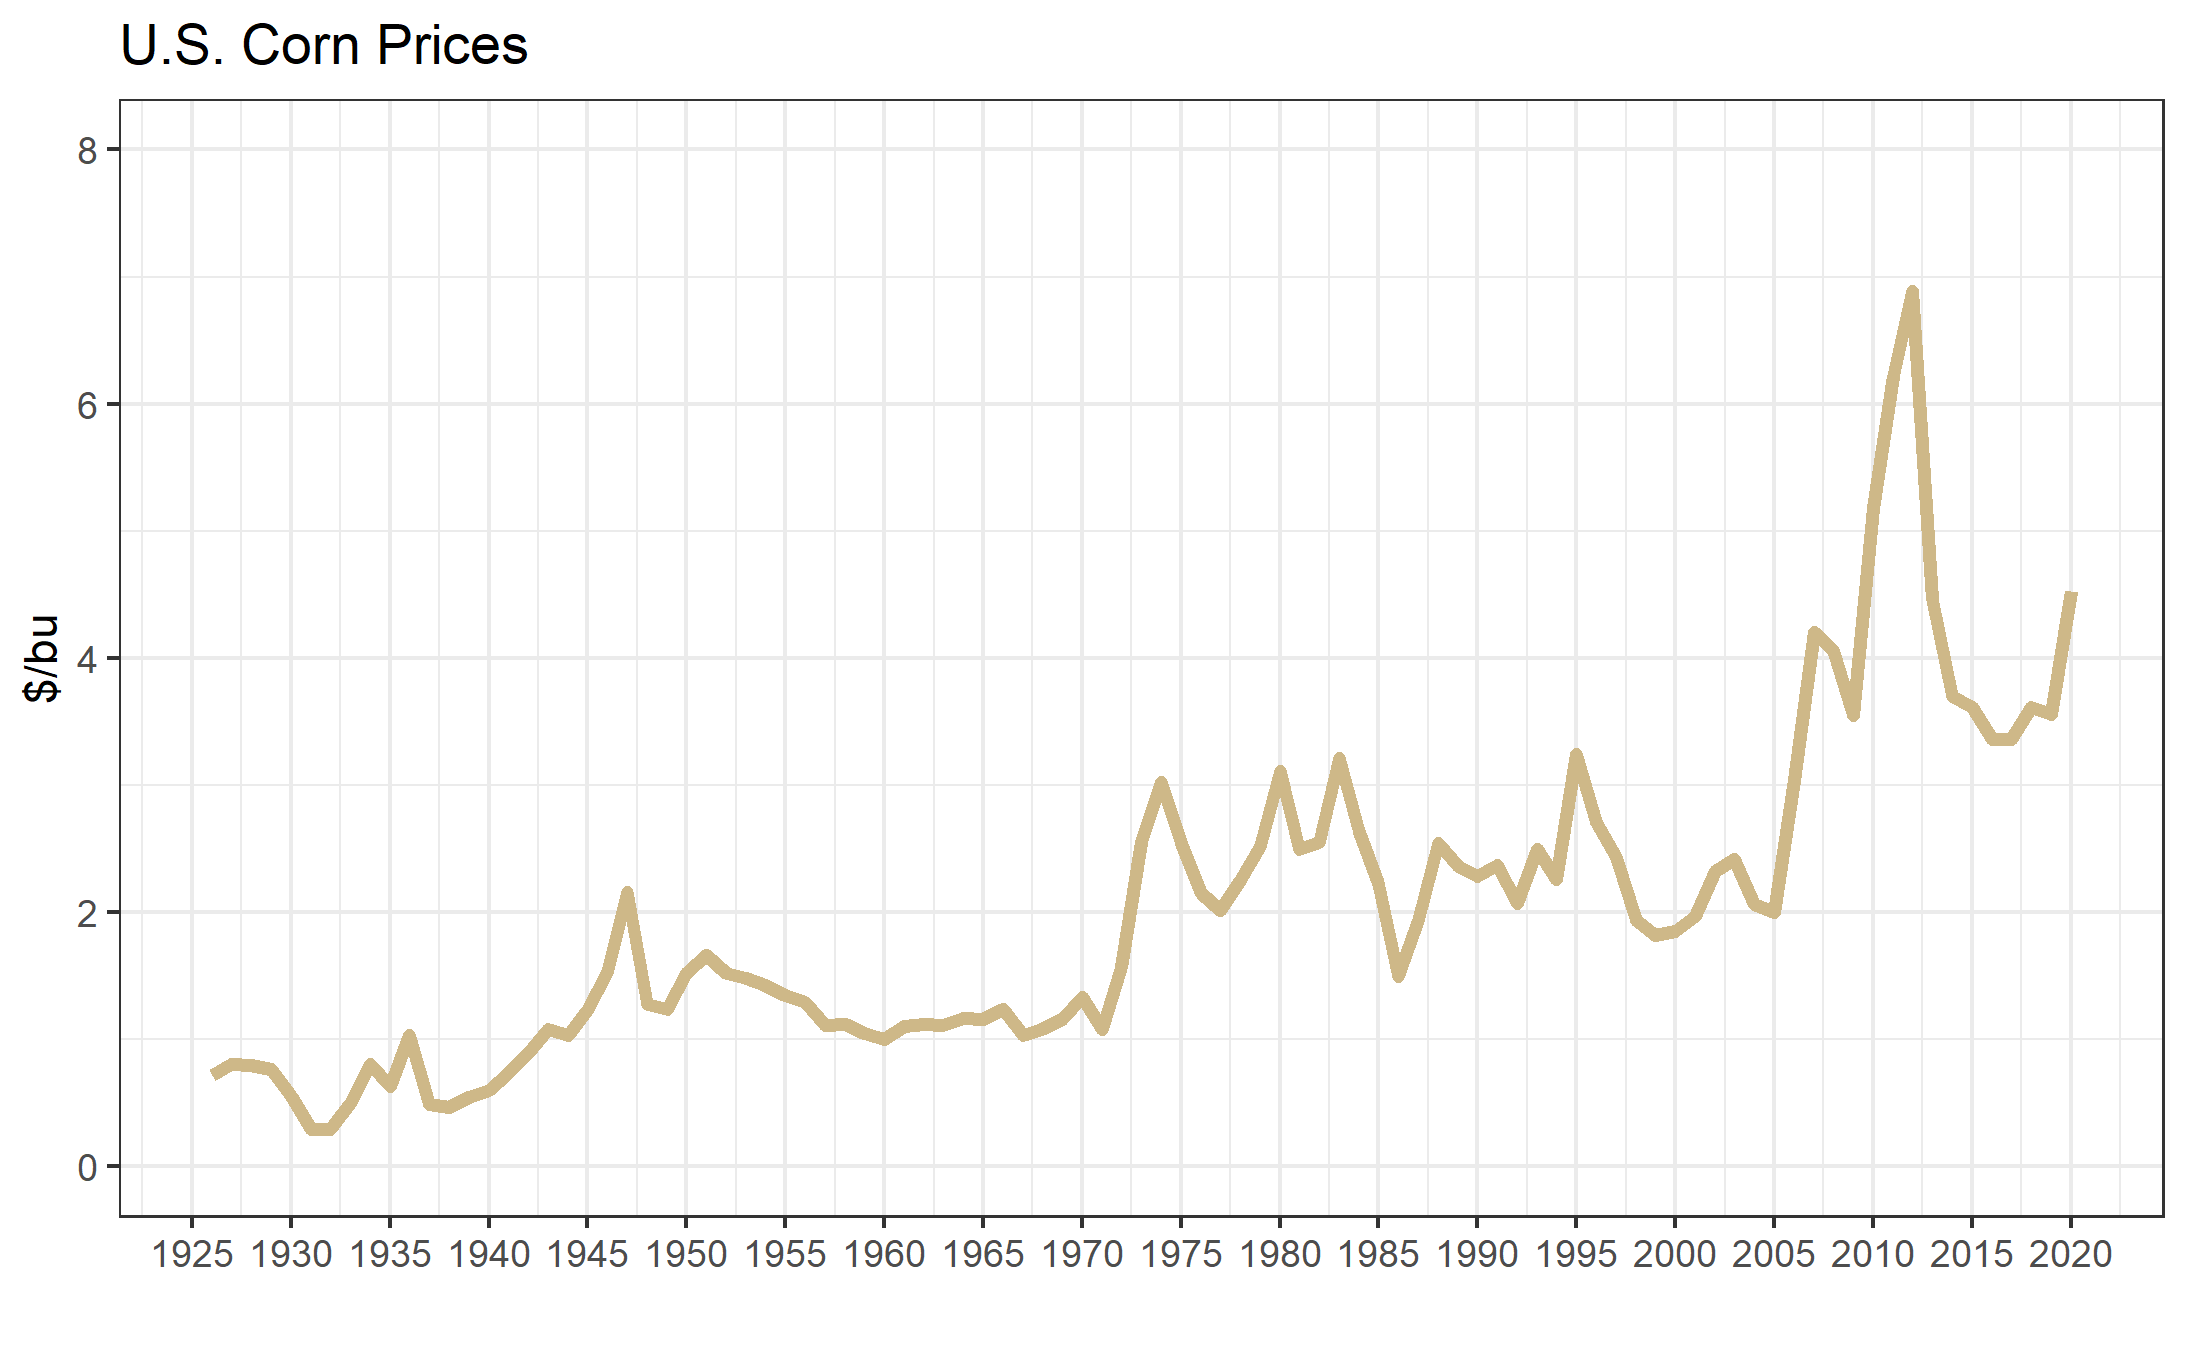
\includegraphics{assets/PrimerforGrain_CornPrices.png}

}

\caption{Corn Prices Long Term}

\end{figure}%

There is a clear run-up in prices in the 1970's and again around
2006-2007. What caused these seemingly permanent price hikes? Make sure
you check out the readings to find out!

\section{Readings}\label{readings}

\begin{description}
\item[\href{pdf-Readings/ers-amber-waves-2009-ag-com-pr-sp-1970s-1990s.pdf}{Agricultural
Commodity Price Spikes in the 1970s and 1990s: Valuable Lessons for
Today}]
This article was published by staff at the United States Department of
Agriculture's Economic Research Service. They look at historical corn
prices and provide some perspective about what caused the price
increases in the 1970's and mid-2000's.
\item[\href{http://www.choicesmagazine.org/magazine/pdf/article_56.pdf}{Market
Instability in a New Era of Corn, Soybean, and Wheat Prices}]
Scott Irwin and Darrel Good had an article in Choices magazine, that
examined the price `eras' we described in this chapter. They also
discuss the causes of the price paradigm shifts. They argued in 2009
that the new `Era' of crop prices were here to stay, and history has
bore this out so far.
\item[\href{http://farmdocdaily.illinois.edu/2016/04/new-era-of-corn-and-soybean-prices.html}{The
New Era of Corn and Soybean Prices Is Still Alive and Kicking}]
Scott Irwin and Darrel Good revisit the price `Era's' discussion again
in April of 2016.
\end{description}

\section{Exercises}\label{exercises}

\begin{enumerate}
\def\labelenumi{\arabic{enumi}.}
\item
  From the readings, describe causes of the rapid and persistent
  increase in prices in the early 1970's.
\item
  From the readings, describe the causes of the rapid and persistent
  increase in prices in 2006/2007.
\item
  In your opinion, is there evidence that price trends will hold at
  their current levels?
\end{enumerate}

\bookmarksetup{startatroot}

\chapter{How to Find Information}\label{how-to-find-information}

{Interested in more? Please let me know by}
\href{https://forms.gle/Q3VByCQZHjfQSy9D7}{taking the survey}!

This chapter serves as an introduction to real-time and historical data
sources, as well as an introduction to the analysts that conduct price
analysis professionally and help us make sense of commodity prices.
First, we will introduce the reader to some entities that provide market
commentary and price analysis. Next, we will provide a very brief
introduction to futures markets as the source of real-time price
information for commodities. This section also covers where and how to
obtain current futures price quotes. In the section that follows we
cover sources for historical data such as the United States Department
of Agriculture and others. These sources will be useful in developing
fundamental price models in later chapters. The goal of this chapter is
to get the reader up to speed on where to get commodity price data and
reading the professional analysis daily. The more you follow commodity
markets, the more you learn. Absorb the insights of the professionals
who live and breath commodity markets every day, and you will begin to
have a feel for what price analysis is all about and how it works.

\section{Market Commentary}\label{market-commentary}

The best way to learn commodity price analysis is to listen to the
professionals who provide commentary on the markets on a regular basis.
Land grant universities located in major commodity producing states all
have components of their outreach programs dedicated to market
commentary. The University of Illinois' web extension program, FARMDOC,
is particularly good. Also, public radio in major commodity producing
areas has excellent coverage. Champaign-Urbana's WILL, and Iowa Public
Televisions' Market to Market are very good. There are \emph{many} other
great sources providing regular commentary, but this will get the reader
started.

\begin{longtable}[]{@{}
  >{\raggedright\arraybackslash}p{(\columnwidth - 4\tabcolsep) * \real{0.1745}}
  >{\raggedright\arraybackslash}p{(\columnwidth - 4\tabcolsep) * \real{0.3490}}
  >{\raggedright\arraybackslash}p{(\columnwidth - 4\tabcolsep) * \real{0.4765}}@{}}
\caption{Table 1. Resources for Commodity Market
Commentary}\tabularnewline
\toprule\noalign{}
\begin{minipage}[b]{\linewidth}\raggedright
Outlet
\end{minipage} & \begin{minipage}[b]{\linewidth}\raggedright
Description
\end{minipage} & \begin{minipage}[b]{\linewidth}\raggedright
Link
\end{minipage} \\
\midrule\noalign{}
\endfirsthead
\toprule\noalign{}
\begin{minipage}[b]{\linewidth}\raggedright
Outlet
\end{minipage} & \begin{minipage}[b]{\linewidth}\raggedright
Description
\end{minipage} & \begin{minipage}[b]{\linewidth}\raggedright
Link
\end{minipage} \\
\midrule\noalign{}
\endhead
\bottomrule\noalign{}
\endlastfoot
Farmdoc Daily & Extension web presence by the department of ACE &
\href{http://farmdocdaily.illinois.edu}{farmdocdaily.illinois.edu} \\
WILL Agriculture & WILL and the University of Illinois Extension &
\href{http://will.illinois.edu/agriculture}{will.illinois.edu/agriculture} \\
Market to Market & Agricultural programming by Iowa Public Television &
\href{http://www.iptv.org/mtom/}{www.iptv.org/mtom/} \\
Center for Commercial Ag & Purdue University Ag Econ &
\url{https://ag.purdue.edu/commercialag/home/} \\
\end{longtable}

\section{Futures Price Quotes}\label{futures-price-quotes}

Futures contracts (contracts to buy/sell a specific quantity of, say,
corn at a specific price on a specific date in the future) can be
distinguished from forward contracts in that quantity and quality are
standardized. This facilitates the ability of futures contracts to be
traded on an exchange. Whereas a forward contract has specific
counter-parties (buyers and sellers), with futures contracts the
exchange becomes the seller to every buyer and the buyer to every
seller. If enough market participants are present it is very easy to get
into and out of these futures contracts because you do not have to come
to an agreement with the original buyer/seller. You simply take an
offsetting position (sell if you originally bought and buy if you
originally sold) at the currently prevailing price. The exchange takes
your contractual obligation off the books and you just pay (or receive)
the difference in price between when you bought and when you sold. Fully
understanding the function of futures markets is well beyond the scope
of this book, but the interested reader is encouraged to refer to Kub
(Kub 2012) for a practical introduction and Hull (Hull 2017) for a more
technical approach.

\subsection{Futures Data Sources}\label{futures-data-sources}

For agricultural commodities in the United States, the
\href{http://www.cmegroup.com/}{CME Group} is the most important futures
exchange for price discovery. Grain and oil-seed contracts traded at the
CME Group include corn, soybeans, soybean oil, soybean meal, soft red
winter wheat, hard red winter wheat. They also list futures contracts
for livestock products such as live cattle, lean hogs, and feeder
cattle. `Soft' commodities that trade on the CME Group are cocoa,
coffee, and sugar. The CME Group also lists energy commodity products
for crude oil, natural gas, ethanol, and other products. This book will
focus most intently on the grain and oil-seed contracts, with some
topics related to the cattle and energy contracts considered. Many of
these futures contracts are considered to be the main price setting
function for the commodity in the world. Chicago Board of Trade (owned
by the CME Group) futures prices of corn and soybeans are considered the
`World Price' of corn and soybeans. Meaning that all over the globe,
prices for these commodities are set based on what the price of corn and
soybeans are trading on the CME Group exchanges.

Real-time (10-min delay) data can be obtained directly from the CME
Group's website. There you can view the most recent quotes, and some
charting capability is provided as well. Typically, however, it is more
convenient to obtain market quotes from third party vendors like
\href{http://www.barchart.com/futures/marketoverview}{barchart},
\href{https://www.tradingview.com/}{TradingView} or others. Those
sources offer a more flexible interface for viewing on the web, and
provide utility to download recent price history.

\subsection{Futures Symbols and Looking up Data by Contract
Expiration}\label{futures-symbols-and-looking-up-data-by-contract-expiration}

Contracts for several different expiry dates trade at the same time.
There is a useful shorthand for finding contracts for a specific
commodity and expiration month that varies only slightly among data
vendors; all follow a general convention for building futures ticker
symbols customizing only to meet the needs of their individual systems.
The table below lists selected grain and oilseed, livestock, and energy
contract symbols, expiration symbols, and common ticker formats used to
search for price quotes. For example, the first row of the table
illustrates that the general convention for representing the CBOT corn
futures contract expiring in December of 2021 is CZ21. The first letter
represents the commodity symbol, C for corn; the second letter
represents the expiration month, Z for December; and the final two
numerals represent the year of expiry, 21for 2021.

\textbf{Some Common Commodity Contract Tickers, with Barchart Ticker
Style}

\begin{itemize}
\item
  Corn, March (H), May (K), July (N), September (U), December (Z),
  \href{https://www.barchart.com/futures/quotes/ZCZ21/overview}{ZCZ21}
\item
  Soybeans, January (F), March (H), May (K), July (N), August (Q),
  September (U), November (X),
  \href{https://www.barchart.com/futures/quotes/ZSX21/overview}{ZSX21}
\item
  HRW Wheat, March (H), May (K), July (N), September (U), December (Z),
  \href{https://www.barchart.com/futures/quotes/KEZ21/overview}{KEZ21}
\item
  SRW Wheat, March (H), May (K), July (N), September (U), December (Z),
  \href{https://www.barchart.com/futures/quotes/ZWZ21/overview}{ZWZ21}
\item
  HRS Wheat, March (H), May (K), July (N), September (U), December (Z),
  \href{https://www.barchart.com/futures/quotes/MWZ21/overview}{MWZ21}
\item
  Live Cattle, Feb (G), Apr (J), Jun (M), Aug (Q), Oct (V), Dec (Z),
  \href{https://www.barchart.com/futures/quotes/LEZ21/overview}{LEZ21}
\item
  Lean Hogs, Feb (G), Apr (J), May (K), Jun (M), Jul (N), Aug (Q), Oct
  (V), Dec (Z),
  \href{httphttps://www.barchart.com/futures/quotes/HEZ21/overview}{HEZ21}
\end{itemize}

Table 3 provides some links to spread charts for commodity spreads we
will cover in this class.

\begin{longtable}[]{@{}
  >{\raggedright\arraybackslash}p{(\columnwidth - 2\tabcolsep) * \real{0.0622}}
  >{\raggedright\arraybackslash}p{(\columnwidth - 2\tabcolsep) * \real{0.9378}}@{}}
\caption{Table 3. Commodity Spreads}\tabularnewline
\toprule\noalign{}
\begin{minipage}[b]{\linewidth}\raggedright
Spread
\end{minipage} & \begin{minipage}[b]{\linewidth}\raggedright
Link
\end{minipage} \\
\midrule\noalign{}
\endfirsthead
\toprule\noalign{}
\begin{minipage}[b]{\linewidth}\raggedright
Spread
\end{minipage} & \begin{minipage}[b]{\linewidth}\raggedright
Link
\end{minipage} \\
\midrule\noalign{}
\endhead
\bottomrule\noalign{}
\endlastfoot
Soybean Crush &
\href{https://www.barchart.com/futures/quotes/ZS*1/technical-chart?plot=LINE&volume=contract&data=DO&density=M&pricesOn=1&asPctChange=0&logscale=0&sym=ZS*1-ZS*2&grid=1&height=500&studyheight=100&isSpread=1}{Barchart
Spread Chart} \\
Cattle Crush &
\href{http://www2.econ.iastate.edu/estimated-returns/Finishing\%20Steer\%20Calves\%20Chart.pdf}{ISU
Spread Calculation}
\href{http://www2.econ.iastate.edu/estimated-returns/}{ISU Livestock
Returns} \\
Corn Crush &
\href{https://www.extension.iastate.edu/agdm/energy/html/d1-10.html}{ISU
Ethanol Grind Margin} (Download Ethanol Profitability spreadsheet. Look
at Grind Margin chart) \\
\end{longtable}

\section{USDA Reports}\label{usda-reports}

The United States Department of Agriculture has a long history of
extensively surveying market conditions, reporting to the public and
maintaining accessible databases. Because of their efforts to provide
consistent and accurate (as is possible) estimates of key variables like
acres planted, yield, production, stocks, consumption, and exports,
market participants follow USDA reports about market conditions very
closely. Their impacts on prices can be seen immediately and sometimes
cause rapid, if not instantaneous price moves as the market digests the
new information from the report. The most closely watched reports are
summarized below.

\subsection{USDA Reports Influential in Commodity
Markets}\label{usda-reports-influential-in-commodity-markets}

\begin{description}
\item[Prospective Plantings]
The Prospective Plantings report is an estimate of grower intentions for
planted acres during the first two weeks of March. The report is
released on the last day of March every year. Planted acres for each
crop varies considerably from year-to-year and this report give the
market important guidance about expected supply of the covered
commodities. The most important reason prospective plantings change from
year-to-year is the relative prices of crops that compete for acres.
Growers look to the prices of futures with a expiry around the time of
harvest for an estimate of expected profit from planting competing
crops. For example, if the price of corn is relatively high compared to
soybeans, and expected profitability from an acre of corn is higher than
from an acre of soybeans, the farmer is likely to shift some of his
planting intentions from soybeans to corn compared to the crop mix
typically planted. In this case you might hear market commentary include
language like, ``\ldots{} corn is bidding for acres.'' Meaning that
price of corn is trying to entice growers to shift acres into corn
production.
\item[Acreage]
While the Prospective Plantings Report estimates growers'
\emph{intentions} to plant, Acreage is an estimate of the acres actually
planted. This report is based on surveys conducted during the first two
weeks of June and released on the last day of June. Weather and changes
in the relative price of crops that compete for acres are the most
important reason for differences between Prospective Plantings and
Acreage reports. Weather can play a factor because crops that compete
for acres are not necessarily planted at the same time. Corn, for
example, is typically planted a few months before soybeans. The Corn
Belt, where the biggest production of corn and soybeans occur, can often
be very wet in the Spring. In some years this makes is physically very
difficult to get to plant the number of acres of corn they intended when
surveyed during the first two weeks of March. The relative price of
crops competing for acres can also change between March and June for any
number of reasons and cause the Acreage report to be substantially
different than Prospective Plantings.
\item[Grain Stocks]
The Grain Stocks report is issued quarterly and contains information
about how much of selected commodities are in storage in the United
States, by state. Information in this report is pertinent to the price
level, as well as the calendar spread between two futures maturities.
When stocks are tight, naturally the price of the commodity will be
high. Also, prices futures contracts soon to expire should exceed those
with longer dated maturities for two reasons. 1) Low prices for distant
futures contracts reflects the tendency for high prices to ration demand
and for future harvests to resolve shortages. 2) Low prices for distant
futures contracts should disincentive storage and bring stocks onto the
market to relieve current shortages. Thus, this report is important both
for price level and spread analysis.
\item[World Agricultural Supply and Demand Estimates (WASDE)]
The WASDE report is released monthly and provides the USDA's forecasts
for U.S. and world supply and use balance sheets for grains, soybeans
and its products, and cotton. It contains supply and use forecasts for
U.S. sugar and livestock commodities. These reports are among the most
important and eagerly anticipated by market participants. The report is
currently released at 12pm EST and release of the report commonly
results in limit price moves in futures markets. It is among the most
involved to prepare. To quote the USDA's own documentation:
\end{description}

\begin{quote}
How the WASDE is Prepared - Lock-up Conditions: To assure the highly
market-sensitive information is released simultaneously to all
end-users, and not prematurely to any one, the WASDE report is prepared
under tight security in a specially designed area of USDA's South
Building. The morning of release, doors in the ``lockup'' area are
secured, window shades are sealed, and telephone and Internet
communications are blocked. Once analysts present their credentials to a
guard, they enter the secured area to finalize the WASDE report.
Communications with the outside world are suspended until the report is
released at 12:00 noon Eastern time.

Source, \href{http://www.usda.gov/oce/commodity/wasde/prepared.htm}{USDA
Office of the Cheif Economist}
\end{quote}

Given the USDA reports' ability to move futures markets, the lock up
condition described in the last paragraph is imperative. The prospect
that USDA reports could be leaked is the inspiration behind the final
scene in \href{https://www.youtube.com/watch?v=1tmI867fAYU}{Trading
Places}, probably the best and only popular movie made about commodity
markets. In this scene, Eddie Murphey and Dan Ackroid's characters learn
that the rich antagonists obtained advance access to the `crop report'
(they do not say which report) pertinent to orange juice futures
containing information that would make the price go down. Eddie Murphey
and Dan Ackroid intercept the information and feed the rich antagonists
a false report with bogus information that would cause the futures price
to rise. Before the report is released the rich antagonists buy A LOT of
orange juice futures contracts, driving the price up. Then Eddie Murphey
and Dan Ackroid start selling when the price is high. When the `crop
report' comes out the price crashes. The rich guys loose a ton of money
and Eddie Murphey and Dan Ackroid become wealthy and retire wealthy to a
tropical paradise.

\begin{description}
\item[Crop Production]
The Crop Production report includes estimates of yield, acres harvested,
and total production for covered commodities. This report is released in
tandem with the WASDE report.
\item[Crop Progress and Condition]
Crop Progress and Condition reports are issued every \textbf{Monday}
during the planting, growing, and harvest season for major crops in the
United States. The weekly updates provide market participants critical
information about the status of the crop. Nass surveys approximately
4,000 individuals in major growing areas familiar with the crops. Check
out one of the weekly tables
\href{http://usda.mannlib.cornell.edu/usda/nass/CropProg//2010s/2017/CropProg-06-19-2017.txt}{June
19, 2017} and summary charts
\href{https://www.nass.usda.gov/Charts_and_Maps/Crop_Progress_&_Condition/2016/US_2016.pdf}{US
Progress and Condition}
\item[Agricultural Marketing Service]
The AMS provides numerous daily and weekly reports related to regional
prices and exports.
\end{description}

\subsection{USDA Data Sources}\label{usda-data-sources}

All of the information contained in the reports described above are
useful for in depth analysis over a long time horizon. As a service the
USDA maintains databases of information contained in historical reports
that are easy to query for analysis. Four important agencies maintaining
databases within the USDA are the
\href{http://www.nass.usda.gov/}{National Agricultural Statistics
Service} (NASS), the
\href{http://apps.fas.usda.gov/psdonline/psdHome.aspx}{Foreign
Agricultural Service} (FAS), the
\href{http://www.ers.usda.gov/data-products.aspx}{Economics Research
Service} (ERS), and the
\href{http://www.ams.usda.gov/market-news/livestock-poultry-grain\#Grain}{Agricultural
Marketing Service}. Each service mentioned here hosts a wide variety of
data and analyses, so concise descriptions are difficult. However some
of the data products commonly used for commodity price analysis are
ACRES PLANTED, PRODUCTION, YIELD, and PRICE RECIEVED by NASS; the
PRODUCTION SUPPLY AND DISTRIBUTION report from FAS (much of the WASDE
report is archived here); COST and RETURNS from ERS; and local prices
from AMS .

\begin{longtable}[]{@{}
  >{\raggedright\arraybackslash}p{(\columnwidth - 2\tabcolsep) * \real{0.1704}}
  >{\raggedright\arraybackslash}p{(\columnwidth - 2\tabcolsep) * \real{0.8296}}@{}}
\caption{Table 3. Summary of USDA Reports and Data
Sources}\tabularnewline
\toprule\noalign{}
\begin{minipage}[b]{\linewidth}\raggedright
Report
\end{minipage} & \begin{minipage}[b]{\linewidth}\raggedright
Link
\end{minipage} \\
\midrule\noalign{}
\endfirsthead
\toprule\noalign{}
\begin{minipage}[b]{\linewidth}\raggedright
Report
\end{minipage} & \begin{minipage}[b]{\linewidth}\raggedright
Link
\end{minipage} \\
\midrule\noalign{}
\endhead
\bottomrule\noalign{}
\endlastfoot
Prospective Plantings &
\href{https://usda.library.cornell.edu/concern/publications/x633f100h?locale=en}{Farmers'
planting intentions} \\
Acreage &
\href{https://usda.library.cornell.edu/concern/publications/j098zb09z}{Planted
Acres} \\
WASDE & \href{https://www.usda.gov/oce/commodity/wasde}{World Supply and
Demand Estimates} \\
Crop Production &
\href{https://usda.library.cornell.edu/concern/publications/tm70mv177?locale=en}{Crop
Production - Acres and Yield} \\
Crop Progress &
\href{https://usda.library.cornell.edu/concern/publications/8336h188j}{Crop
Progress} \\
NASS & \url{http://www.nass.usda.gov/} \\
FAS & \url{http://www.fas.usda.gov/data} \\
ERS &
\href{http://www.ers.usda.gov/data-products.aspx}{http://www.ers.usda.gov} \\
AMS &
\href{http://www.ams.usda.gov/market-news/livestock-poultry-grain\#Grain}{http://www.ams.usda.gov/} \\
\end{longtable}

\section{Conclusion}\label{conclusion}

This concludes chapter 3. We learned resources for accessing commodity
market data, USDA reports, and daily market commentary. Aimed with these
resources one can begin to follow the ups and downs of commodity prices
and get a feel for how fundamental supply and demand factors cause
fluctuations in prices. In the next section we will cover fundamental
analysis in detail. Fundamental analysis is driven by building balance
sheets for components of supply and demand. Using the balance sheet
approach, the analyst attempts to forecast the price that will cause
quantities supplied and quantities demanded to be equal. This market
equilibrium, if the fundamental model is correctly specified, should be
a reasonable forecast of price.

\section{Readings}\label{readings-1}

\begin{description}
\item[\href{http://farmdocdaily.illinois.edu/2015/03/usda-stocks-and-acreage-estimates-for-soybeans-and-corn.html}{USDA
Stocks and Acreage Estimates Smaller than Expected for Soybeans and
Larger than Expected for Corn}]
Good discusses the release of the March 31st, 2015 \emph{Grain Stocks}
and \emph{Prospective Plantings} reports. Notice the attention paid to
the difference between the USDA report numbers and the ``Trade's
Guess''. Why is this important?

Good, D. ``USDA Stocks and Acreage Estimates Smaller than Expected for
Soybeans and Larger than Expected for Corn.'' farmdoc daily (5):59,
Department of Agricultural and Consumer Economics, University of
Illinois at Urbana-Champaign, March 31, 2015.
\item[\href{http://farmdocdaily.illinois.edu/2015/10/progression-usda-corn-and-soybean-acreage-estimates.html}{Progression
of USDA Corn and Soybean Acreage Estimates and Prospects for Final
Estimates for 2015}]
Irwin and Good provide a thorough description of the procedures used by
the USDA to determine acreage estimates for the Prospective Plantings,
Acreage, Crop Production, and Grain Stocks reports.

Good, D., and S. Irwin. ``Progression of USDA Corn and Soybean Acreage
Estimates and Prospects for Final Estimates for 2015.'' farmdoc daily
(5):191, Department of Agricultural and Consumer Economics, University
of Illinois at Urbana-Champaign, October 15, 2015.
\end{description}

\section{Exercises}\label{exercises-1}

\begin{enumerate}
\def\labelenumi{\arabic{enumi}.}
\item
  Find data on Quandl.com for the December 2015 CBOT corn futures
  contract (Note: linked above). Download the data in a .csv or
  Microsoft Excel file. Do the same for the March and May 2015 CBOT corn
  futures contract and put the price series together in one excel file
  (Be sure the dates line up.) Now, graph all three prices together.

  \begin{itemize}
  \tightlist
  \item
    Are the price equal?
  \item
    Why not if the represent the same thing?
  \item
    Conjecture what are the determinants of the price orderings of these
    contracts.
  \end{itemize}
\item
  Calculate the difference between the December price and the March
  price in excel. This difference is called the spread. Sometimes you
  will hear it referred to as the Dec/March spread or the z/h spread -
  only making reference to the contract month codes. Convention dictates
  that the nearest to expire contract is the first in the difference;
  i.e., \texttt{December\ -\ March} rather than
  \texttt{March\ -\ December}.

  \begin{itemize}
  \tightlist
  \item
    From a forecasting perspective, does it seem like price level is
    easier to predict, or the price spread?
  \item
    Can you think of any statistics you could calculate to back up your
    intuition?
  \end{itemize}
\item
  From the readings for this chapter, what do you suppose is the
  significance of the USDA report compared to the ``Trade's Guess''?
\end{enumerate}

\bookmarksetup{startatroot}

\chapter{Futures and Hedging Review}\label{futures-and-hedging-review}

{Interested in more? Please let me know by}
\href{https://forms.gle/Q3VByCQZHjfQSy9D7}{taking the survey}!

\textbf{Highlights}

\begin{itemize}
\tightlist
\item
  Review of futures contracts and how to calculate profit or loss on a
  trade.
\item
  Hedging examples from the sell side (farmer's hedge) and from the buy
  side (flour mill's hedge).
\item
  Learn how basis risk impacts a hedge.
\end{itemize}

\textbf{Check your Understanding}

\begin{itemize}
\tightlist
\item
  Can you calculate the profit or loss from a trade?
\item
  Can you fill out a hedging net revenue table given prices on key
  dates?
\end{itemize}

This chapter is a review of the basics of hedging. What is its purpose?
Who does it? And how do futures contracts facilitate a `hedge'?

Merriam-Webster defines a `hedge' as a means of protection or defense
(as against a financial loss). Hedging in the sense of hedging with a
futures contract, is exactly that a defense against a financial loss. In
the present context, a hedge is the use of a derivative contract to
reduce or eliminate risk in your business' profits.

Understanding who is hedging and why is very helpful to understanding
price relationships and what drives them to move up or down.

\section{Futures Contract Review}\label{futures-contract-review}

A futures contract is a contract between two parties to buy and sell at
an agreed to price, a specific quantity and quality of something at a
specific location. In the case of CBOT corn futures, it is 5,000 bushels
of U.S. number 2 yellow corn, at specific elevators along the Illinois
River, Lake Michigan, or associated canals. These contracts are traded
on a centralized exchange, similar to the `stock market', and the two
counter-parties do not know each other. The difference between a futures
contract, and say buying a stock, is that when the trade takes place, no
ownership transfer occurs. It is simply a promise to buy or sell at a
specific date in the future. That is why there are many different
futures contract `months' like `December 2017' corn futures, and `March
2018' corn futures. Traders on futures exchanges need to post `margin'
which is just an amount of money that acts as a performance bond so that
everyone has confidence that both parties can make good on the contract
if it is held until the futures contract expires. As the price moves up,
the seller's position is losing (because selling `low' is `bad'
business), and some money is taken from their margin account and put
into the buyer's margin account (because buying `low' is `good'
business). This daily transfer of money from the losers to the winners
is called `marking to market', and it makes sure everyone has the
financial capital required to make good on the terms of the contract.

Consider this example. At 10am the March corn futures contract is
trading at \$4.50 per bushel. Trader A decides to buy one contract and
Trader B decides to sell one contract. At 1pm both traders decide to
close their position and the price has moved up to \$4.75 per bushel.
Since the price went up the by \$0.25 per bushel, the longs (buyers)
gain \(+0.25*5000 = \$1250\) and the shorts (sellers) lose
\(-0.25*5000 = \$1250\).

\begin{longtable}[]{@{}
  >{\raggedright\arraybackslash}p{(\columnwidth - 4\tabcolsep) * \real{0.2800}}
  >{\raggedright\arraybackslash}p{(\columnwidth - 4\tabcolsep) * \real{0.3600}}
  >{\raggedright\arraybackslash}p{(\columnwidth - 4\tabcolsep) * \real{0.3600}}@{}}
\toprule\noalign{}
\begin{minipage}[b]{\linewidth}\raggedright
Time
\end{minipage} & \begin{minipage}[b]{\linewidth}\raggedright
Trader A
\end{minipage} & \begin{minipage}[b]{\linewidth}\raggedright
Trader B
\end{minipage} \\
\midrule\noalign{}
\endhead
\bottomrule\noalign{}
\endlastfoot
10am & buy \$4.50 & sell \$4.50 \\
1pm & sell \$4.75 & buy \$4.75 \\
profit per bu & \$4.75 - \$4.50 = +\$0.25 & \$4.50 - \$4.75 = -\$0.25 \\
profit one contract & +\$1250 & -\$1250 \\
\end{longtable}

Very few contracts are held all the way to expiration when transfer of
ownership would take place. The traders who originally bought, sometime
before expiration will sell, eliminating their obligation in the market,
or getting them to a `flat' position. The traders who originally sold,
will buy, getting them to a `flat' position as well. The rest of the
chapter will cover how exactly these futures contracts can facilitate a
hedge for different types of businesses.

\subsection{Delivery}\label{delivery}

The CME Group grain and oilseed future are deliverable contracts,
ensuring a link between the spot market and the futures market. Only a
few of the futures contracts traded are actually delivered on, however.
The purpose of the futures market is not to provide a mechanism for
physical exchange, but rather a means for streamlined risk management in
a liquid market. That said, there is always some contracts that end up
being held by the long and the short side of the trade into delivery. We
will discuss briefly the mechanism the CME Group grain and oilseed
contracts for delivery.

The exchange has designated a few large commercial grain handlers and
warehouses as \emph{regular for delivery}. These grain handlers lie in
one of the following territories specified in the
\href{https://www.cmegroup.com/rulebook/CBOT/II/10/10.pdf}{CME Group
Rulebook}

\begin{quote}
Corn shipping certificates shall specify shipment from one of the
warehouses or shipping stations currently regular for delivery and
located in one of the following territories:

A. Chicago and Burns Harbor, Indiana Switching District - When used in
these Rules, the Chicago Switching District will be that area
geographically defined by Tariff ICC WTL 8020-Series and that portion of
the Illinois Waterway at or above river mile 304 which includes the
Calumet Sag Channel and the Chicago Sanitary \& Ship Canal. When used in
these Rules, Burns Harbor, Indiana Switching District will be that area
geographically defined by the boundaries of Burns Waterway Harbor at
Burns Harbor, Indiana which is owned and operated by the Indiana Port
Commission.

B. Lockport-Seneca Shipping District - When used in these Rules, the
Lockport-Seneca Shipping District will be that portion of the Illinois
Waterway below river mile 304 at the junction of the Calumet Sag Channel
and the Chicago Sanitary \& Ship Canal and above river mile 244.6 at the
Marseilles Lock and Dam.

C. Ottawa-Chillicothe Shipping District - When used in these Rules, the
Ottawa-Chillicothe Shipping District will be that portion of the
Illinois Waterway below river mile 244.6 at the Marseilles Lock and Dam
and at or above river mile 170 between Chillicothe and Peoria, IL.

D. Peoria -- Pekin Shipping District - When used in these Rules, the
Peoria-Pekin Shipping District will be that portion of the Illinois
Waterway below river mile 170 between Chillicothe and Peoria, IL and at
or above river mile 151 at Pekin, IL.
\end{quote}

If someone with a short futures position wants to deliver on their
futures contract they cannot just show up at one of these locations with
5,000 bushels of grain in trucks. The actual thing that can be delivered
is referred to as a \emph{shipping certificate} for 5,000 bushels of
grain from a regular for delivery warehouse. This is a certificate
giving the holder the right to demand load-out of grain that meets
certain quality standards. Since the shipping certificates represent
physical bushels in storage at these regular for delivery warehouses,
and warehouse space is not free, holders of shipping certificates are
required to pay what are called \emph{premium charges}. Premium charges
are simply fees collected by the warehouse for the space provided to
store the grain. The exchange specifies that premium charges for corn
and soybeans shall not exceed 0.165 cents per bushel per day, or about
4.95 cents per bushel per month. We will need to use the premium charges
on shipping certificates in Chapter 5 when we introduce the concept of
\emph{Financial Full Carry}.

Likewise, if the long party (the person who bought the futures contract)
wants to take delivery, they must pay the full amount,
\(Futures Price X 5,000\) bushels, and must pay premium charges to the
warehouse to hold the shipping certificate.

\section{Examples: Who Hedges and How Does a Futures Contract Facilitate
a
Hedge?}\label{examples-who-hedges-and-how-does-a-futures-contract-facilitate-a-hedge}

\subsection{Farmer}\label{farmer}

Consider the corn farmer who plants her crop in April waits for it to
grow and then mature through the summer and fall, then harvests it in
November. If the farmer sells right after harvest in the cash market,
she will very likely take her grain to a local grain elevator (similar
to the one pictured below), where the elevator will purchase all she has
at a price they publicly offer anyone interested in selling grain.

Figure 1. A Grain Elevator in Royal, IL

\href{https://commons.wikimedia.org/wiki/File:Grain_elevators_in_Royal,_IL.}{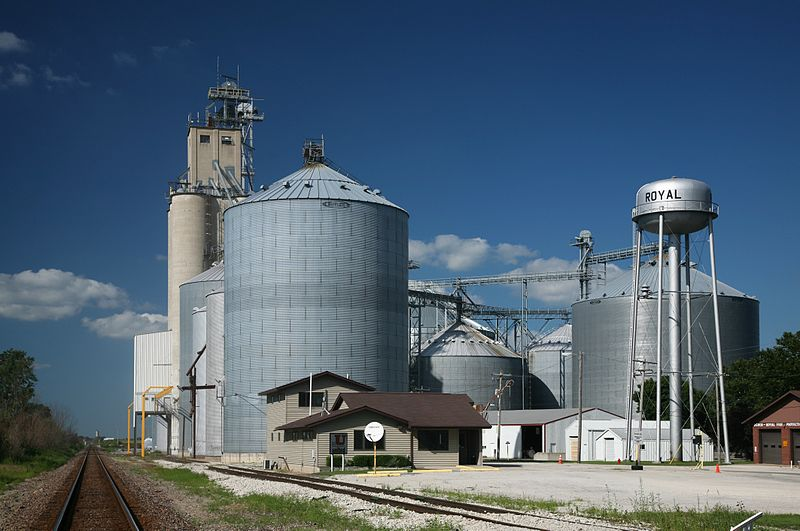
\includegraphics{assets/Grain_elevator_royal_IL.jpg}}

Source:
\href{https://commons.wikimedia.org/wiki/File\%3AGrain_elevators_in_Royal\%2C_IL.jpg}{Daniel
Schwen, CC-License}

The farmer's entire income for the year will come from the sale of this
grain, and a lot can happen to the price of corn between April and
November, leaving the farmer exposed to tremendous income risk. Many
farmers desire the ability to reduce this income risk by entering into a
contractual relationship that reduces the uncertainty in the income they
receive. Currently there are several ways they can achieve this.

\begin{enumerate}
\def\labelenumi{\arabic{enumi}.}
\item
  Crop Insurance. They can purchase a crop insurance policy that will
  pay them an indemnity if either price goes down, yield is low, or both
  depending on the exact specification of the contract. This activity
  does not directly interact with the futures market, so it does not
  have a large effect on price.
\item
  Forward Price Contract. Local grain elevators (sometimes called
  merchandisers) typically offer forward contracts to buy grain from
  farmers. Along with the cash price they post publicly on a daily
  basis, they will post forward `bids'. The forward contract simply
  states that the farmer will deliver a certain quantity of grain to
  that elevator within a specific date range, usually a window of a few
  weeks. Upon delivery, the elevator will pay the farmer the price
  agreed to (the forward bid price) on the date they entered int the
  forward contract together. This eliminates price uncertainty for the
  farmer, as long as the elevator does not go bankrupt before the
  delivery date of the contract, they will have the forward bid price
  with certainty. The forward contract transfers price risk to the
  elevator. The elevator does not want to entertain price risk during
  this time either, but the elevator has a contract to buy the grain at
  a specific price, but the price at which they can turn around and sell
  it to someone else is uncertain. They will transfer the price risk to
  speculators in the futures market by selling futures. So farmers
  entering into forward contracts with local grain merchandisers
  ultimately results in selling of futures contracts by the grain
  merchandisers. We will see in an examples below how exactly selling
  futures eliminates price risk.
\item
  Futures Market. Alternatively, a farmer could go directly to the
  futures market themselves to sell futures contracts and reduce price
  uncertainty. This reduces, but not eliminates uncertainty because the
  farmer still faces basis risk in this case. A detailed example will
  help explain how this works.
\end{enumerate}

Suppose on May 1st, the farmer's local elevator is offering to buy corn
for \$3.50, and the May futures contract is trading at \$3.60. Since the
May futures contract is about to expire, the cash price and Futures
price are not separated by much time (we have discussed briefly how
prices through time along the futures forward curve provide incentives
to store) and thus should not be very different because of time.
However, the local elevator's price can differ from the Futures price
because they are at different locations. For example, the elevator in
the photo at Royal, IL is about 116 miles from the `regular for
delivery' elevators in the Calmet-Sag Chanel near Orland Park, IL. The
\$0.10 difference between the May futures price and the cash price on
May 1st in Royal, IL is largely due to the geographic distance between
the two locations. The price distance over space is called the basis.
Basis can be computed compared to any of the futures contracts, but it
makes sense to consider basis compared to the futures contract that
corresponds to the planned cash sale.

\[Basis = Cash Price - Futures Price\]

Also on May 1st, the December futures contract price is \$3.75. If the
farmer wants to reduce price uncertainty they will sell futures,
sometimes referred to as `selling forward' or `selling ahead'.

\textbf{To Hedge - Take the same action in the futures market (buy or
sell) that you will do in the cash market at a future date}

The farmer will sell corn in the cash market in November, so to hedge
she should sell (the December) futures to hedge. This concept is called
being natually long. Since the farmer is essentially long the
unharvested grain in the field (after all, `long' is a financial
position that gains value when price goes up and loses value when price
goes down). Therefore, to hedge, they need to take a position with the
opposite profile, i.e., they should take a short position to hedge their
naturally long position.

Consider two cases, one where the Dec futures price in November turned
out to be \$4.00, and one where the Dec futures price in November turned
out to be \$3.60.

\textbf{Dec Futures Price went Up to \$4.00, Basis Unchanged}

\begin{longtable}[]{@{}
  >{\centering\arraybackslash}p{(\columnwidth - 8\tabcolsep) * \real{0.1721}}
  >{\centering\arraybackslash}p{(\columnwidth - 8\tabcolsep) * \real{0.2787}}
  >{\centering\arraybackslash}p{(\columnwidth - 8\tabcolsep) * \real{0.2049}}
  >{\centering\arraybackslash}p{(\columnwidth - 8\tabcolsep) * \real{0.2213}}
  >{\centering\arraybackslash}p{(\columnwidth - 8\tabcolsep) * \real{0.1230}}@{}}
\toprule\noalign{}
\begin{minipage}[b]{\linewidth}\centering
Date
\end{minipage} & \begin{minipage}[b]{\linewidth}\centering
Action
\end{minipage} & \begin{minipage}[b]{\linewidth}\centering
Cash Price in Royal, IL
\end{minipage} & \begin{minipage}[b]{\linewidth}\centering
Dec Corn Futures Price
\end{minipage} & \begin{minipage}[b]{\linewidth}\centering
Basis
\end{minipage} \\
\midrule\noalign{}
\endhead
\bottomrule\noalign{}
\endlastfoot
May 1st & Sell Dec Futures & \$3.50 & \$3.75 & -\$0.25 (Dec) \\
Nov 1st & Buy Dec Futures \& Sell Cash Corn & \$3.75 & \$4.00 & -\$0.25
(Dec) \\
Profit Calculation, & Cash and Futures & \$3.75 & \$3.75 - \$4.00 =
-\$0.25 & \\
& Net per bushel revenue & \$3.75 - \$0.25 & = \$3.50 & \\
\end{longtable}

With the basis unchanged, the farmer eliminated the uncertainty over the
price at which she will sell her crop. By `selling ahead' in the futures
market, the price was locked in, except for the basis. Note that in this
case, the farmer would have liked to be able to sell for \$3.75 instead
of \$3.50 net, but by locking in the price with futures she gave up the
potential for upside. In the next example, though, we show the
advantage. In the next example, prices go down between May and November,
and the futures hedge protects the farmer from these deteriorating
prices.

\textbf{Dec Futures Price went Down to \$3.60, Basis Unchanged}

\begin{longtable}[]{@{}
  >{\centering\arraybackslash}p{(\columnwidth - 8\tabcolsep) * \real{0.1721}}
  >{\centering\arraybackslash}p{(\columnwidth - 8\tabcolsep) * \real{0.2787}}
  >{\centering\arraybackslash}p{(\columnwidth - 8\tabcolsep) * \real{0.2049}}
  >{\centering\arraybackslash}p{(\columnwidth - 8\tabcolsep) * \real{0.2213}}
  >{\centering\arraybackslash}p{(\columnwidth - 8\tabcolsep) * \real{0.1230}}@{}}
\toprule\noalign{}
\begin{minipage}[b]{\linewidth}\centering
Date
\end{minipage} & \begin{minipage}[b]{\linewidth}\centering
Action
\end{minipage} & \begin{minipage}[b]{\linewidth}\centering
Cash Price in Royal, IL
\end{minipage} & \begin{minipage}[b]{\linewidth}\centering
Dec Corn Futures Price
\end{minipage} & \begin{minipage}[b]{\linewidth}\centering
Basis
\end{minipage} \\
\midrule\noalign{}
\endhead
\bottomrule\noalign{}
\endlastfoot
May 1st & Sell Dec Futures & \$3.50 & \$3.75 & -\$0.25 (Dec) \\
Nov 1st & Buy Dec Futures \& Sell Cash Corn & \$3.35 & \$3.60 & -\$0.25
(Dec) \\
Profit Calculation, & Cash and Futures & \$3.35 & \$3.75 - \$3.60 =
+\$0.15 & \\
& Net per bushel revenue & \$3.35 + \$0.15 & = \$3.50 & \\
\end{longtable}

By selling Dec futures ahead of the cash sale, price risk was reduced.
It was reduced, but not eliminated because by hedging with futures there
is still basis risk. The next examples show what happens when the basis
is uncertain. Consider now that the futures price was unchanged in
November, that is in November the Dec futures is still trading at
\$3.80. Now however, consider two cases. The basis widens to -\$0.50,
and the basis narrows to \$0.00.

\textbf{Dec Futures Price Unchanged, Basis now -\$0.50}

\begin{longtable}[]{@{}
  >{\centering\arraybackslash}p{(\columnwidth - 8\tabcolsep) * \real{0.1721}}
  >{\centering\arraybackslash}p{(\columnwidth - 8\tabcolsep) * \real{0.2787}}
  >{\centering\arraybackslash}p{(\columnwidth - 8\tabcolsep) * \real{0.2049}}
  >{\centering\arraybackslash}p{(\columnwidth - 8\tabcolsep) * \real{0.2213}}
  >{\centering\arraybackslash}p{(\columnwidth - 8\tabcolsep) * \real{0.1230}}@{}}
\toprule\noalign{}
\begin{minipage}[b]{\linewidth}\centering
Date
\end{minipage} & \begin{minipage}[b]{\linewidth}\centering
Action
\end{minipage} & \begin{minipage}[b]{\linewidth}\centering
Cash Price in Royal, IL
\end{minipage} & \begin{minipage}[b]{\linewidth}\centering
Dec Corn Futures Price
\end{minipage} & \begin{minipage}[b]{\linewidth}\centering
Basis
\end{minipage} \\
\midrule\noalign{}
\endhead
\bottomrule\noalign{}
\endlastfoot
May 1st & Sell Dec Futures & \$3.50 & \$3.75 & -\$0.25 (Dec) \\
Nov 1st & Buy Dec Futures \& Sell Cash Corn & \$3.25 & \$3.75 & -\$0.50
(Dec) \\
Profit Calculation, & Cash and Futures & \$3.25 & \$3.75 - \$3.75 =
+\$0.00 & \\
& Net per bushel revenue & \$3.25 + \$0.00 & = \$3.25 & \\
\end{longtable}

This time, the basis widening from -\$0.25 to -\$0.50 was a loss to the
farmer, even though general price levels were unchanged (Dec price
unchanged). The next example shows the farmer's revenue if the basis
strengthens, or narrows.

\textbf{Dec Futures Price Unchanged, Basis now \$0.00}

\begin{longtable}[]{@{}
  >{\centering\arraybackslash}p{(\columnwidth - 8\tabcolsep) * \real{0.1721}}
  >{\centering\arraybackslash}p{(\columnwidth - 8\tabcolsep) * \real{0.2787}}
  >{\centering\arraybackslash}p{(\columnwidth - 8\tabcolsep) * \real{0.2049}}
  >{\centering\arraybackslash}p{(\columnwidth - 8\tabcolsep) * \real{0.2213}}
  >{\centering\arraybackslash}p{(\columnwidth - 8\tabcolsep) * \real{0.1230}}@{}}
\toprule\noalign{}
\begin{minipage}[b]{\linewidth}\centering
Date
\end{minipage} & \begin{minipage}[b]{\linewidth}\centering
Action
\end{minipage} & \begin{minipage}[b]{\linewidth}\centering
Cash Price in Royal, IL
\end{minipage} & \begin{minipage}[b]{\linewidth}\centering
Dec Corn Futures Price
\end{minipage} & \begin{minipage}[b]{\linewidth}\centering
Basis
\end{minipage} \\
\midrule\noalign{}
\endhead
\bottomrule\noalign{}
\endlastfoot
May 1st & Sell Dec Futures & \$3.50 & \$3.75 & -\$0.25 (Dec) \\
Nov 1st & Buy Dec Futures \& Sell Cash Corn & \$3.75 & \$3.75 & \$0.00
(Dec) \\
Profit Calculation, & Cash and Futures & \$3.75 & \$3.75 - \$3.75 =
+\$0.00 & \\
& Net per bushel revenue & \$3.75 + \$0.00 & = \$3.75 & \\
\end{longtable}

The narrowing of the basis was an increase in profit to the farmer.

These examples show why it is said that when a farmer hedges with
futures they are `long in the basis'. a futures hedge eliminates price
uncertainty that comes from general price levels:

\begin{itemize}
\tightlist
\item
  If prices go up, they receive an increase in the cash price they
  receive, but a loss on their futures position
\item
  If prices go down, they receive less in cash price when they sell corn
  in their local market, but a gain on their futures position.
\end{itemize}

The futures hedge, however, does not protect against changes (good or
bad) in the relative price in their local cash market and the futures
price.

\begin{enumerate}
\def\labelenumi{\arabic{enumi}.}
\setcounter{enumi}{3}
\tightlist
\item
  Options Market. They could also use options on futures contracts to
  reduce downside risk, but maintain upside potential profits.
  Specifically, a farmer could buy a put option for a premium paid
  upfront. The put option makes money if the price goes down, like a
  short (sold) futures position, but if the price goes up, it does not
  lose any more than the original premium paid. Therefore, if the price
  goes down, she is hedged, but if the price goes up, she will enjoy
  increased profits.
\end{enumerate}

\subsection{Flour Mill}\label{flour-mill}

A flour mill buys large quantities of grain for making into flour. They
can use futures to hedge price risk by `buying ahead' futures contracts.
Remember that a futures hedge always involves making a trade in the
futures contract that is the same as what you will do in the cash
market. In this case, the flour mill buys grain, so their futures hedge
should buy futures. Since the flour mill likely wants to process grain
year round, they need to hedge price risk at multiple points in time to
correspond to when they routinely purchase grain. For example, high
commercial wheat flour mills can process upwards of 50,000 bushels of
wheat per month. With wheat futures contracts specified for 5,000
bushels they need 10 wheat futures contracts to hedge their wheat buying
for one month.

There are five wheat futures contracts per year, March, May, July,
September, and December

\begin{longtable}[]{@{}lccccc@{}}
\toprule\noalign{}
Wheat Futures Contracts & & & & & \\
\midrule\noalign{}
\endhead
\bottomrule\noalign{}
\endlastfoot
Expiration & March & May & July & September & December \\
\end{longtable}

If the mill buys wheat at the first of every month, they will have to
use the nearest contract month to hedge price. For example, to hedge a
purchase of wheat on February 1st, the mill will have to use the March
futures expiration, because there is no February contract and the March
contract is the closest expiration. Then suppose on December 1st the
mill wants to lock in its wheat purchase price (aside from basis risk)
for the first six months of the next year. Then, for example, it will
have to hedge January, February, and March wheat purchases with the
March futures contract. Since they buy 50,000 bushels per month, which
is equivalent to 10 contracts per month, they will need to buy 60
contracts of wheat on Dec 1 to hedge January through July purchases.
Hedges should be lifted simultaneously with activity in the cash market.
For example, on January 1st the mill will purchase 50,000 bushels to
process for the month of January in the cash market. Then they should
lift their hedge on 10 contracts, or sell 10 contracts also on January
first. This means after January 1st, the mill is still holding 20 long
March futures contracts (they are `long' 20 contracts) which keeps
February and March's purchases hedged. The table below details the mills
activities in the spot market and futures market throughout the year. It
takes real data from 2016, and assumes that the basis is fixed at -0.25
cents under the nearby futures contract, meaning the spot price column
is always 0.25 cents less than the next to expire futures contract.

\begin{longtable}[]{@{}
  >{\centering\arraybackslash}p{(\columnwidth - 14\tabcolsep) * \real{0.0827}}
  >{\centering\arraybackslash}p{(\columnwidth - 14\tabcolsep) * \real{0.2105}}
  >{\centering\arraybackslash}p{(\columnwidth - 14\tabcolsep) * \real{0.1805}}
  >{\centering\arraybackslash}p{(\columnwidth - 14\tabcolsep) * \real{0.2556}}
  >{\centering\arraybackslash}p{(\columnwidth - 14\tabcolsep) * \real{0.0602}}
  >{\centering\arraybackslash}p{(\columnwidth - 14\tabcolsep) * \real{0.0677}}
  >{\centering\arraybackslash}p{(\columnwidth - 14\tabcolsep) * \real{0.0677}}
  >{\centering\arraybackslash}p{(\columnwidth - 14\tabcolsep) * \real{0.0752}}@{}}
\toprule\noalign{}
\begin{minipage}[b]{\linewidth}\centering
Dates
\end{minipage} & \begin{minipage}[b]{\linewidth}\centering
Action
\end{minipage} & \begin{minipage}[b]{\linewidth}\centering
Long
\end{minipage} & \begin{minipage}[b]{\linewidth}\centering
Net Price Paid
\end{minipage} & \begin{minipage}[b]{\linewidth}\centering
Spot
\end{minipage} & \begin{minipage}[b]{\linewidth}\centering
Mar Fut
\end{minipage} & \begin{minipage}[b]{\linewidth}\centering
May Fut
\end{minipage} & \begin{minipage}[b]{\linewidth}\centering
Jul Futs
\end{minipage} \\
\midrule\noalign{}
\endhead
\bottomrule\noalign{}
\endlastfoot
Dec 1, 15 & Buy 30 Mar, 20 May, 10 Jul & & & 469.75 & 470 & 476.5 &
483.25 \\
Jan 1, 16 & Buy 50k spot, Sell 10 Mar & 20 Mar, 20 May, 10 Jul & -479 +
(479.25-470) = - 469.75 & 479.00 & 479.25 & 485 & 490.5 \\
Feb 1 & Buy 50k spot, Sell 10 Mar & 10 Mar, 20 May, 10 Jul & -444.75 +
(445-470) = -469.75 & 444.75 & 445 & 453.25 & 460.25 \\
Mar 1 & Buy 50k spot, Sell 10 Mar & 20 May, 10 Jul & -471.25 +
(471.5-470) = -469.75 & 471.25 & 471.5 & 473.5 & 480.75 \\
Apr 1 & Buy 50k spot, Sell 10 May & 10 May, 10 Jul & -477.75 + (478-
476.5) = -476.25 & 477.75 & NA & 478 & 488.5 \\
May 1 & Buy 50k spot, Sell 10 May & 10 Jul & -464.75 + (465 -476.5) =
476.25 & 464.75 & NA & 465 & 464.5 \\
Jun 1 & Buy 50k spot, Sell 10 Jul & 0 & -431 + (431.25- 483.25) = -483 &
431 & NA & NA & 431.25 \\
\end{longtable}

The `crush' hedges are a little more complicated because they involve
buying a certain kind of commodity, transforming it, and selling another
commodity. Some are lucky in that they can hedge both the buy and sell
side of the crushing business.

\subsection{Soybean Crusher}\label{soybean-crusher}

The soybean crusher buys soybeans and sells soybean meal and oil. Their
futures hedge would involve buying soybean futures and selling meal and
oil futures.

\subsection{Importance of Having a Line of Credit in Futures
Hedging}\label{importance-of-having-a-line-of-credit-in-futures-hedging}

Anyone who is hedging with futures -- whether they be farmers, flour
mills, or commercial grain handlers -- must have a line of credit in
place to meet margin calls in the event that the market is moving
against their hedge. For example, the farmer sells futures as a hedge
against her cash sale at a later date. If the price starts moving up,
the grain she will sell in the cash market is worth more, but the
futures hedge is losing money. As the short hedge is losing money,
margin needs to be maintained in their hedging account. If prices move
against the hedge a lot, additional money will need to be deposited to
keep sufficient margin in the account. Usually, this will need to come
from a lender. The lender knows it is a safe loan because prices are
going up, the cash sale will cover any losses in the futures account.
Without the ability to access a line of credit and maintain margin, the
short hedge position will be forced to liquidate, and then the farmer
will no longer be hedged.

\subsection{How Crop Revanue Insurance Has Changed Commodity Marketing
and Hedging
Needs}\label{how-crop-revanue-insurance-has-changed-commodity-marketing-and-hedging-needs}

\bookmarksetup{startatroot}

\chapter{Introduction to Option
Contracts}\label{introduction-to-option-contracts}

{Interested in more? Please let me know by}
\href{https://forms.gle/Q3VByCQZHjfQSy9D7}{taking the survey}!

\textbf{Highlights}

\begin{itemize}
\item
  Learn the basics of call and put options
\item
  Learn what is moneyness and how it affects option prices
\item
  Learn about intrinsic value of options
\end{itemize}

\textbf{Check your Understanding}

\begin{itemize}
\item
  Which option has a `high' premium, an in-the-money or an
  out-of-the-money option?
\item
  Does a long put position have unlimited upside potential? What about a
  long call position?
\item
  Suppose you are a farmer with unpriced grain that you will harvest in
  October. Why would why would a long put option be a hedge?
\end{itemize}

\section{What is an Option Contract?}\label{what-is-an-option-contract}

The previous chapter provided an introduction to futures markets and how
they can be used to hedge a position in the cash market, or to speculate
if you have conviction about the direction of price movement in the
future. In this chapter, we introduce options contracts. An option
contract gives the holder the right, but not the obligation to a
position in the underlying contract by a certain date
(\textbf{hull2017?}). That means that every option contract is tied to
another asset or financial instrument. The purchaser of an option
contract will accept the position in the underlying only if it is
advantageous to do so.

\subsection{Call Options Vs Put
Options}\label{call-options-vs-put-options}

There are two basic types of options: call options and put options. Call
options give the holder the \emph{right to buy} the underlying at a
specified price (known as the strike price) by the expiration date of
the option contract. Put options give the holder the \emph{right to
sell} the underlying at the strike price by the expiration date.
Standard call and put options are most commonly one of two types, either
American or European. American options can be exercised at any time
(meaning the holder of the option contract may take the long position in
the underlying asset at any time prior to or at expiration). Whereas, a
European contract can only be exercised at the option contract's
expiration.

\subsection{Option Contract
Components}\label{option-contract-components}

All option contracts must specify the following details.

\begin{itemize}
\item
  \textbf{Expiration Date}: The date at which the option contract either
  must be exercised or left to expire worthless. Sometimes call
  maturity.
\item
  \textbf{Strike Price}: The strike price defines the price at which the
  holder may buy the underlying (in the case of a call option) or the
  price at which the holder may sell the underlying (in the case of a
  put option). Sometimes call exercise price.
\item
  \textbf{Exercise}: To exercise the option is to elect to take the
  position in the underlying (buy at the strike for a call option or
  sell at the strike for a put option).
\item
  \textbf{Underlying}: The asset or financial instrument on which the
  option is based. In the case of our class we will be talking about
  options on futures contracts.
\item
  \textbf{Premium}: Purchasers of an option must pay a price upfront to
  the seller, called the option premium. This is because the inherent
  right, but not obligation of an option contract means that they hold a
  position with no downside risk. An upfront payment, the price or
  premium of the option is required to entice sellers to trade these
  contracts.
\end{itemize}

\section{What are the Obligations of Option
Sellers?}\label{what-are-the-obligations-of-option-sellers}

Every option contract has a buyer and a seller. We discussed how the
buyer of the option has the right, but not the obligation to buy (for a
call option) or sell (for a put option). Once an option seller has taken
the position, they have certain obligations, namely to deliver a long
position to the call buyer or deliver a short position to the put buyer.

\textbf{Call Option Seller:} The call option seller must be ready to
deliver a long position in the underlying to a call option buyer. That
means that they must be ready to sell the underlying at the strike
price. Notice, that the rational call buyer will only exercise if the
price of the underlying is above the strike price of the option
contract. The call option seller hopes that the price of the underlying
stays below the strike price and they get to keep the premium without
having to be assigned a losing position in the underling.

\textbf{Put Option Seller:} The put option seller is in a similar
situation as the call option seller. The put option seller must be ready
to buy the underlying at the strike price. The rational put option buyer
will only exercise their option if the price of the underlying is below
the strike price. Therefore, the put option seller hopes that the price
of the underlying stays above the strike price so they are paid the
option premium without getting assigned to a losing position in the
underlying.

\section{\texorpdfstring{\textbf{Profit and Loss Diagrams for Option
Positions}}{Profit and Loss Diagrams for Option Positions}}\label{profit-and-loss-diagrams-for-option-positions}

The preceding discussion containing a lot of descriptions can be quite
wordy. In this case, a picture really is worth a thousand words. In the
figure below we plot the profit diagram for long and short positions of
both a call and put option. For simplicity, we plot both the call and
put options with an equal premium. In the next chapter we will learn
that call and put options with the same strike have a very specific
relationship (and it is not that the prices are equal), but for now it
helps create a simple example.

The specifics:

\begin{itemize}
\item
  Strike = 450.00 cents
\item
  Premium = 10 cents
\end{itemize}

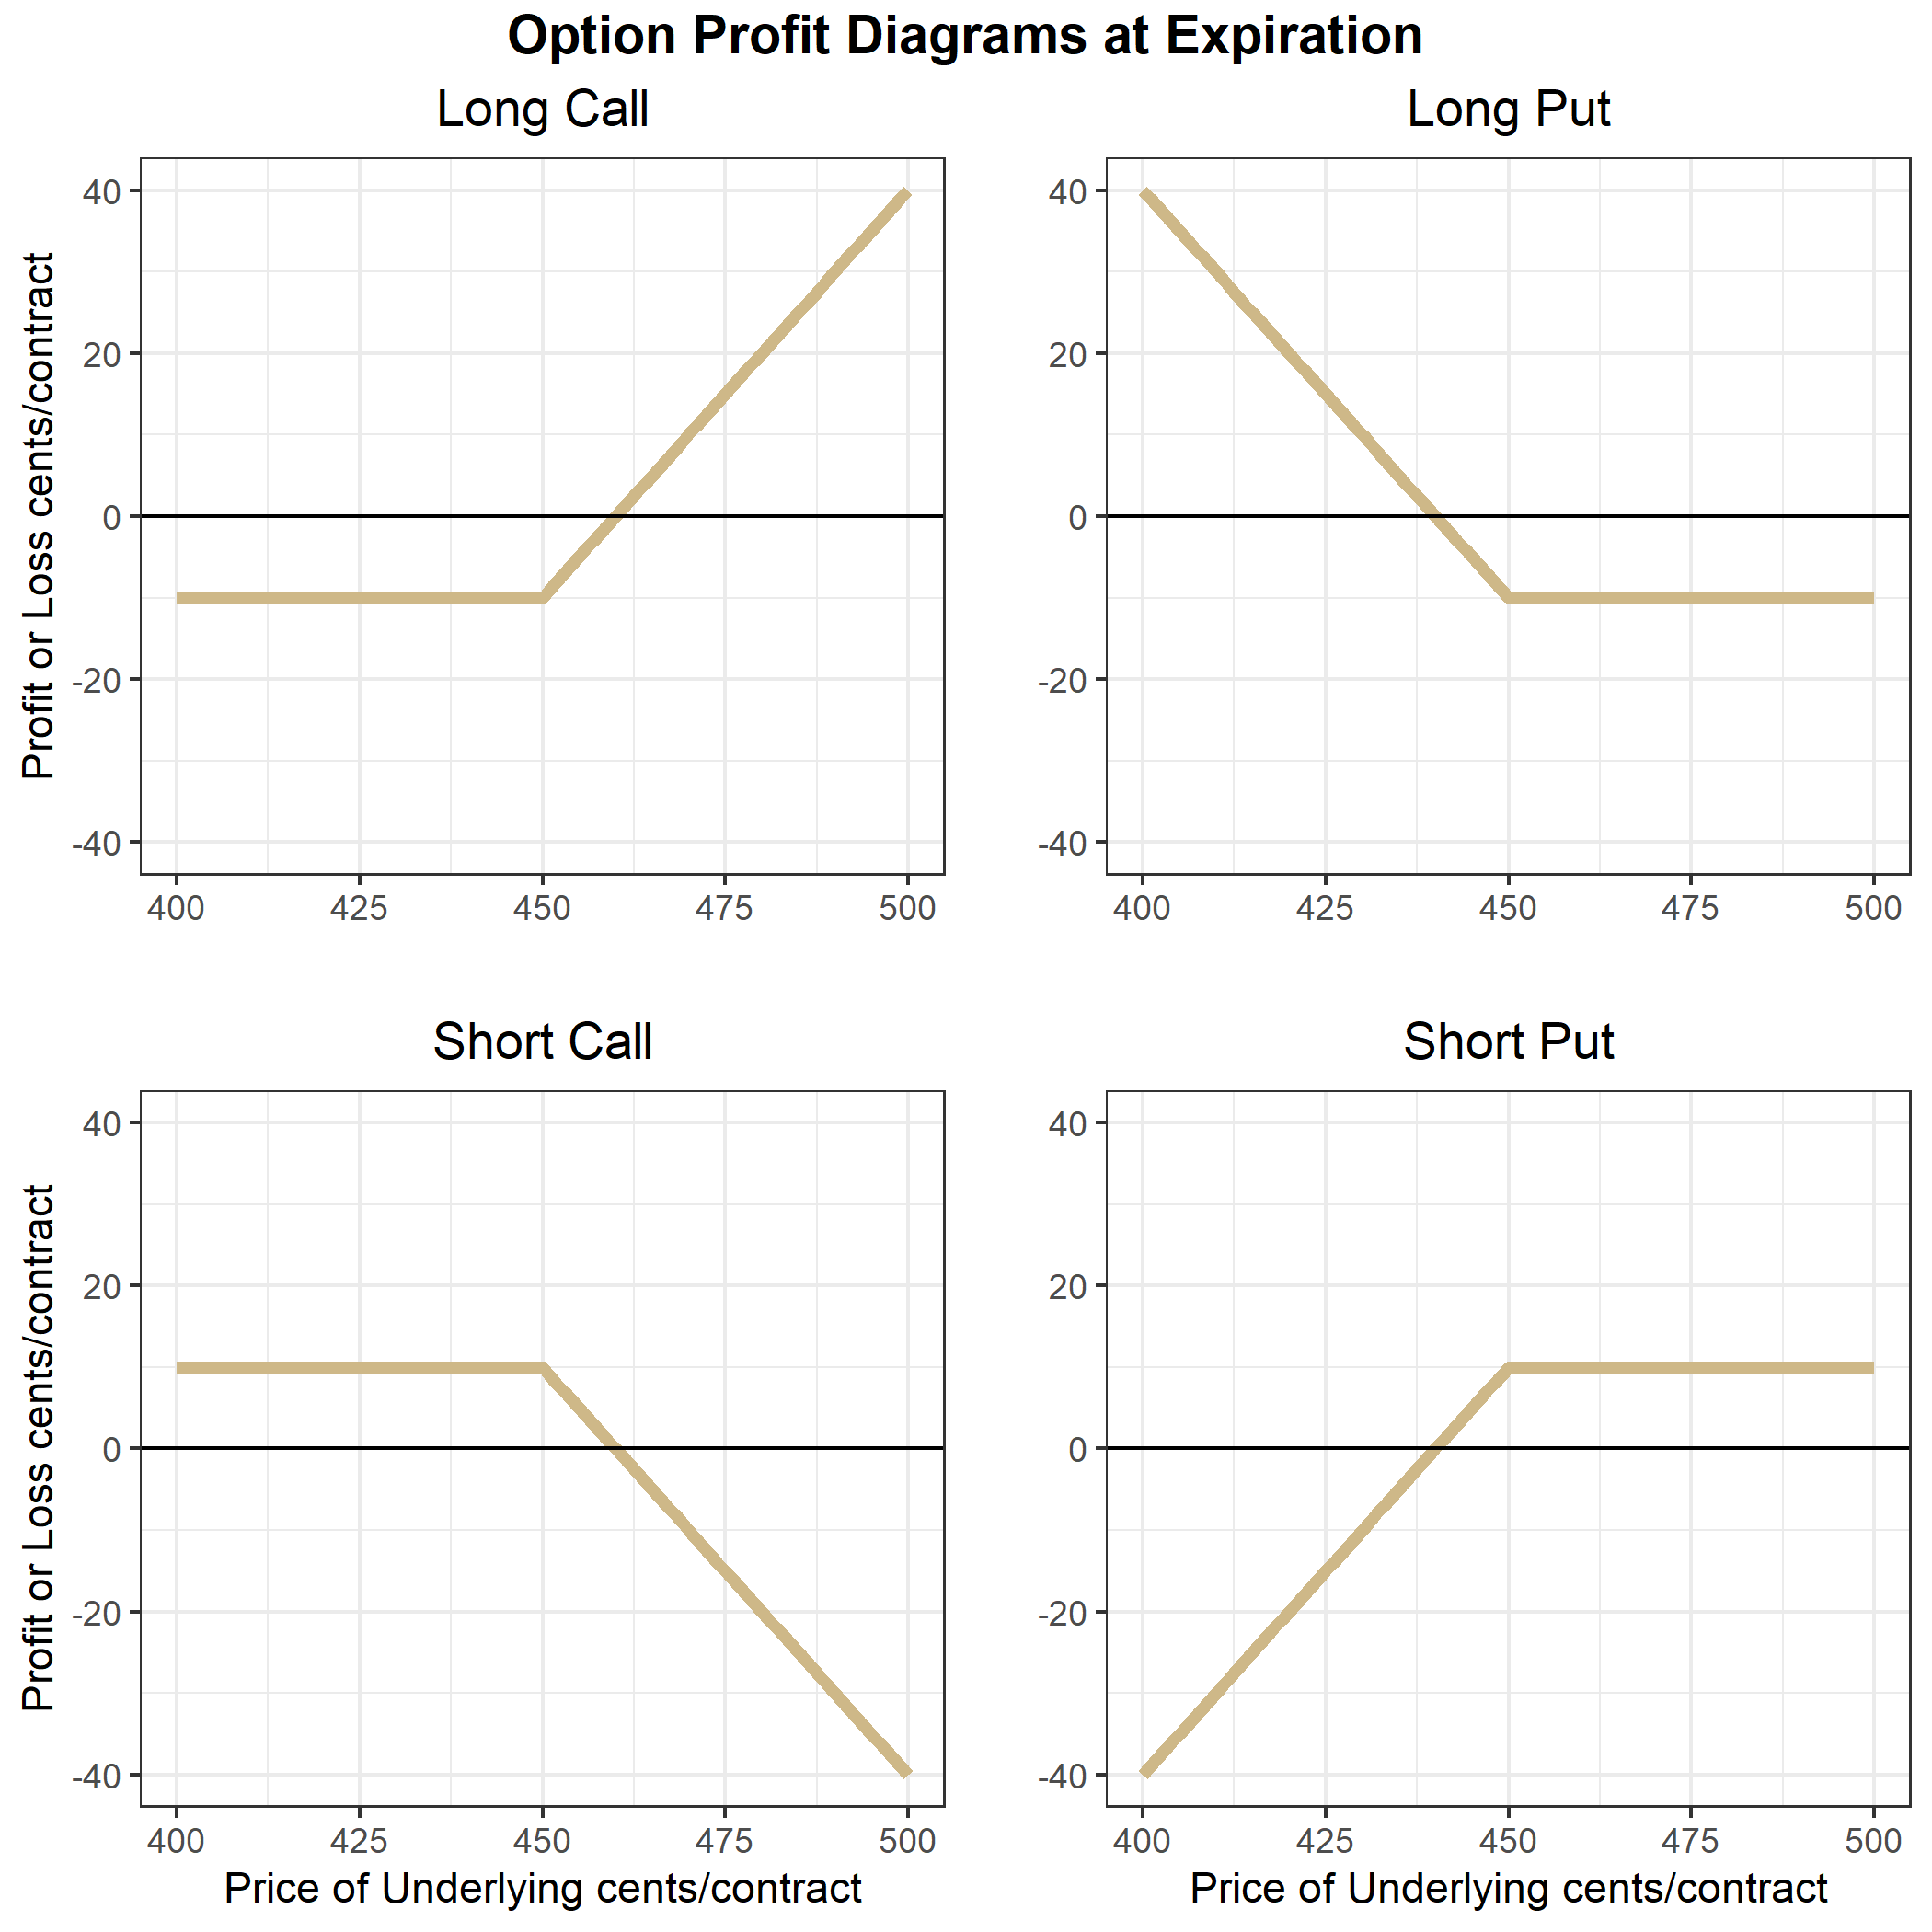
\includegraphics{assets/Options1-optionplot.png}

Option profit diagrams are often referred to as hockey stick diagrams
for obvious reasons. Take a look at the long call figure. A long call
position's downside risk is limited to the price paid for the option. If
the price of the underlying contract falls below 450 and stays there
until expiration, then the option expires worthless and the long call
holder's profit is -10 cents * size of the contract. For example, if
this were a call option on a corn futures contract whose size is 5,000
bushels then Profit = -10*5000 = 50,000 cents or \$500. If the price of
the underlying rises higher than 460, the position is in positive profit
territory.

Similarly for the long put position. A put with strike price = 450 gives
the holder the right to sell for 450. So if the price of the underlying
expires above 450, the holder of the long put option position will have
profit of -10*size of the contract. The long put option position has a
breakeven point at 440 cents, and has positive profit if the price of
the underlying falls below 440 cents at expiration.

The short call position is a mirror image of the long call position
along the x axis. This position provides the holder with 10 cent profit
at expiration if the price of the underlying is below 450 cents. The
profit is declining from 450 to 460 cents, and begins losing money when
the price of the underlying is above 460 cents at expiration.

Similarly for the short put position, with the short put position having
10 cents profit when the price is above 450 cents at expiration, and
losing money when the price is below 440 cents at expiration.

The key observation being that long option positions have nearly
unlimited upside potential, but require an upfront cost, while short
option positions receive payment upfront in the form of the option
premium in exchange for taking the downside risk.

\section{Moneyness of an Option}\label{moneyness-of-an-option}

Option contracts are often characterized by their
\emph{\textbf{moneyness}.} Moneyness simply refers to how near the price
of the underlying is to the strike price. We say an option is deep
\textbf{out-of-the money} if the price of the underlying is far below
the strike of a call option and far above the strike of a put option
(basically when the price of the underlying is in the flat part of the
option profit diagrams). We say an option is deep \textbf{in-the-money}
when the price of the underlying is far above the strike of the call
option and far below the strike of the put option (when the price of the
underlying falls in the sloped part of the option profit diagram).
Finally, we say an option is \textbf{at-the-money} or
\textbf{near-the-money} when the price of the underlying is near the
kink of the option profit diagram.

Getting a feel for these definitions will help you develop intuition for
options prices in the next chapter. In-the-money options should be
expensive and out-of-the-money options should be cheap.

\section{Option Prices (Premium)}\label{option-prices-premium}

Option prices (also called option premium) are determined by buyers and
sellers in options markets, usually in electronic limit order books
similar to other assets available to trade like stocks or futures
contracts. It helps to think about option contracts like insurance
policies. When you buy insurance for your car you pay a small amount at
the beginning of the policy period in exchange for an agreement from
your insurance company that they will pay damages in the (hopefully
unlikely) event that you crash your car. You buy the insurance to
protect yourself financially in the event you need to unexpectedly
replace your car. Over your lifetime of car ownership you will probably
pay more in car insurance than you collect in insurance claims. But for
most of us, the comfort of not having to worry about a surprise \$20K
expenditure is worth it. The insurance company makes money year over
year because they set premiums in such a way that they take in more
premium than they pay out in claims. Insurance companies employ armies
of actuaries and statisticians to calculate the probability you will
crash our car and the actuarily fair rate (which is probability of a
crash time what they have to pay you if you crash). Then the insurance
company adds enough to cover business overhead and a profit margin, and
that is how your car insurance rate is determined.

Option buyers are like you and options sellers are like the insurance
company in the car insurance example. Except in the case of options
premiums, market participants are continually assessing what each option
contract's premium should be. Given the current price of the underling
asset, volatility levels in the market, time to expiration of the
contract, and some other things, what is the probability the contract
will expire in the money? What is a fair price for a position in the
market with limited downside risk and unlimited upside potential? In the
next chapter we will learn the basics of option pricing and the most
famous (though imperfect) option pricing model, but we can use a concept
called intrinsic value to get a sense of some properties option prices
should have.

\subsection{Intrinsic Value}\label{intrinsic-value}

If we take the profit diagrams for the long call and put positions above
and just plot what the gain or loss in the underlying market would be if
we exercised right now, they would look similar to the plots above,
except not shifted down by the amount of the option premium. This plots
the intrinsic value of the options, or how much the position would be in
profit if it were exercised immediately.

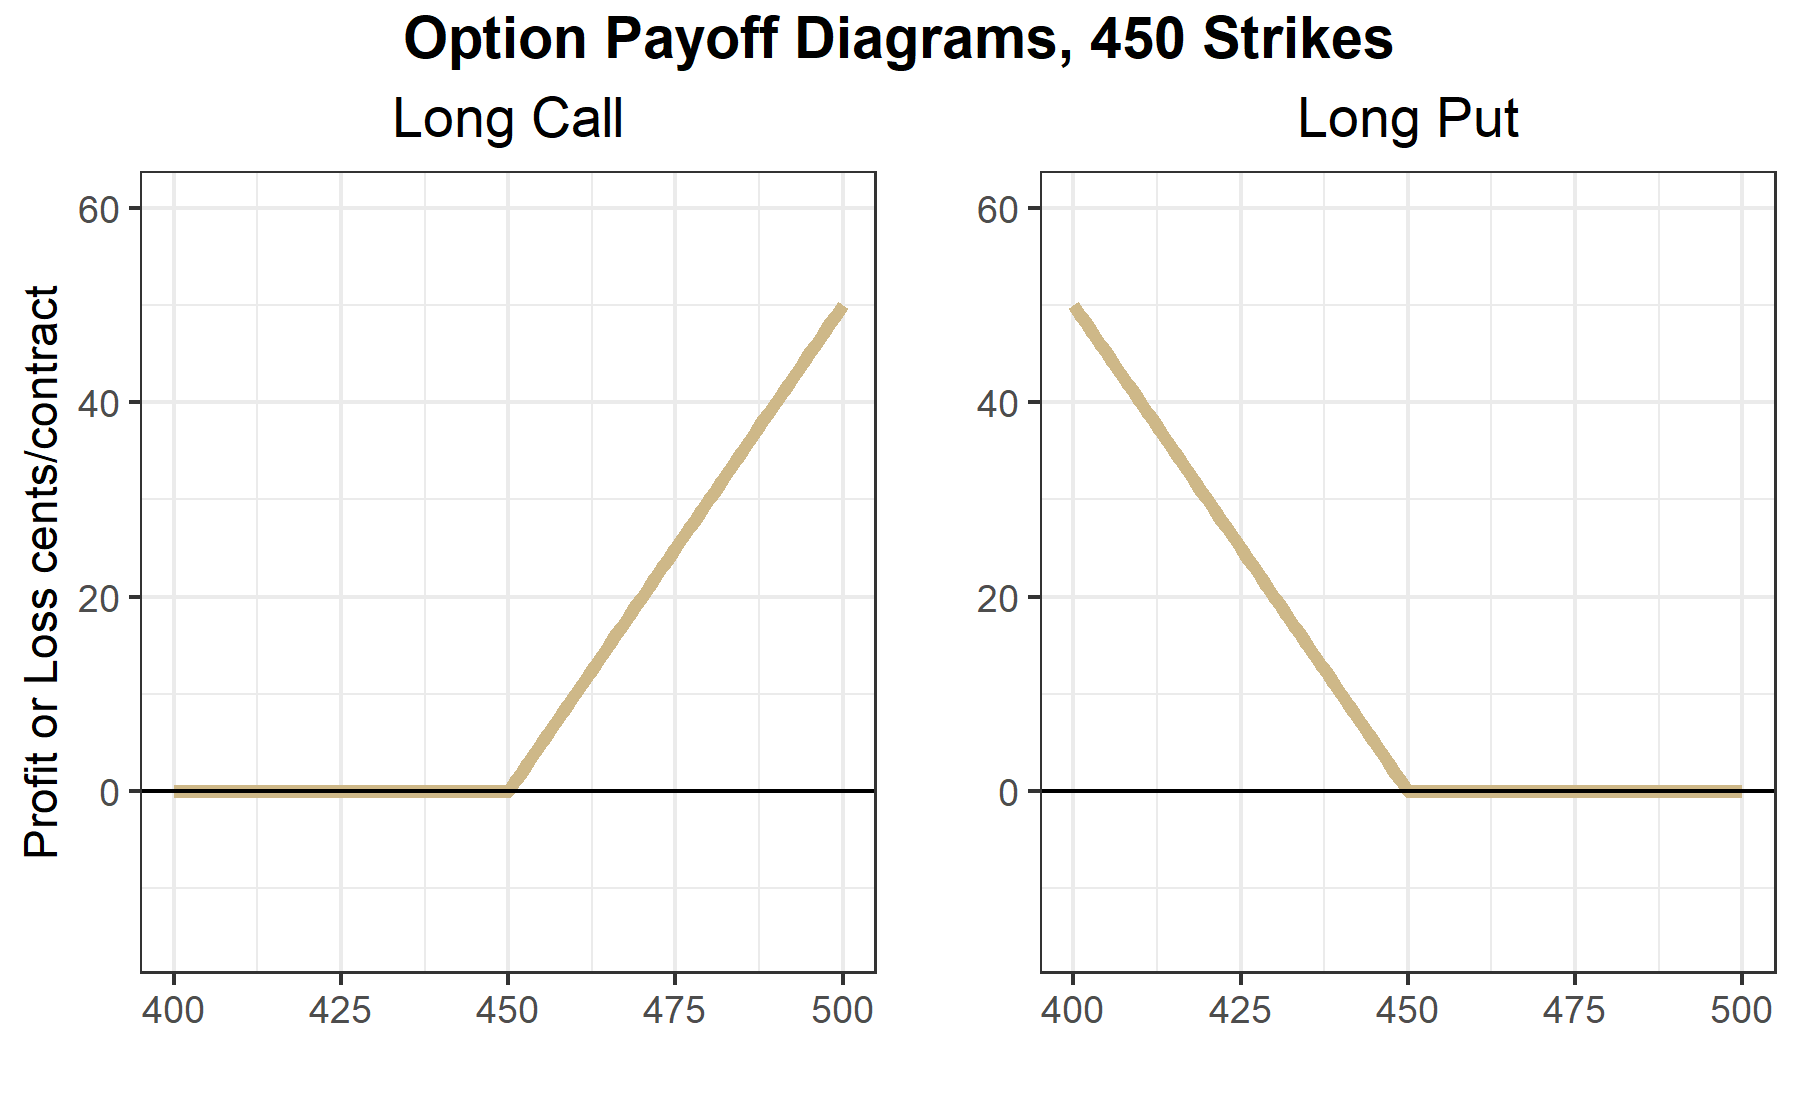
\includegraphics{assets/Options1-optionintrinsic.png}

The options should be worth at least as much as its intrinsic value.
Otherwise and arbitrage opportunity would exist. You could buy the
option, exercise immediately, and immediately offset your position in
the underlying for a riskless profit. For this reason, option prices
usually fall somewhat above the intrinsic value diagram, as a function
of the price of the underlying along the x-axis. How far above is
determined by several factors that we will learn about in the next
chapter.

\section{Margin Requirements}\label{margin-requirements}

Since long option positions require premium to be paid upfront, the
option buyer literally prepays the entire risk of the position.
Therefore, no additional margin is required. Option sellers on the other
hand, have large downside exposure so those positions require margin to
be posted. The amount is determined by the exchange that offers the
option contract for trading (with some brokers requiring even more than
set by the exchange). The amount of margin required is set at the
discretion of the exchange, but is greatly influenced by both recent and
historical volatility of that particular market.

\section{Size of the Underlying}\label{size-of-the-underlying}

Every option contract will specify how much of the underlying the
contract is associated with. In the case of stock options, options most
frequently are for 100 shares of the underlying. So if you buy 1 call
option with a premium of \$1.00 and a strike of \$120 on company XYZ
\$2.00, for example, you have purchased the right to buy 100 shares of
XYZ at a price of \$120. Making the actual cost to buy the option
\(100*1.00 = \$100\).

The size units for options on futures contracts are typically just for
one futures contract, though. So if you buy a call option on soybean
futures at the \url{cmegroup.com} it is the right to buy just one
futures contract.

\section{Reading Option Quotes}\label{reading-option-quotes}

The figure below shows quotes for several options on the January 2021
soybeans futures contract that trades on the \url{cmegroup.com}
exchange. The underlying contract information is in the top table. In
the LAST column we see that last price the contract had traded for at
the time I took a snapshot of these quotes. CHANGE shows the price
change since the PRIOR SETTLE price, which is the settlement price from
the previous day. HIGH price, LOW price, and VOLUME on the trading
session are also provided.

Recall that soybeans are quoted to the eight of a cent, so the 1249'0
means \(1249 + \frac{0}{8} = 1249.00\) cents. While the PRIOR SETTLE
price of 1243'6 means \(1243 + \frac{6}{8} = 1243.75\) cents.

Most providers of option contract quotes will organize the information
in a similar way as shown below. Calls and Puts are shown in major
columns, organized by ascending strike prices, which are usually
displayed in the middle of the table for easy reference whether you are
focused on Call or Put options.

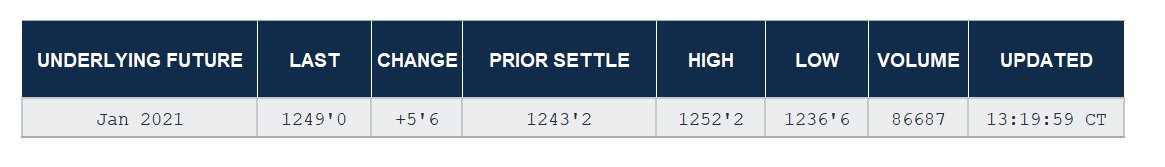
\includegraphics{assets/Options1-undelyingquote.PNG}

\begin{figure}[H]

{\centering 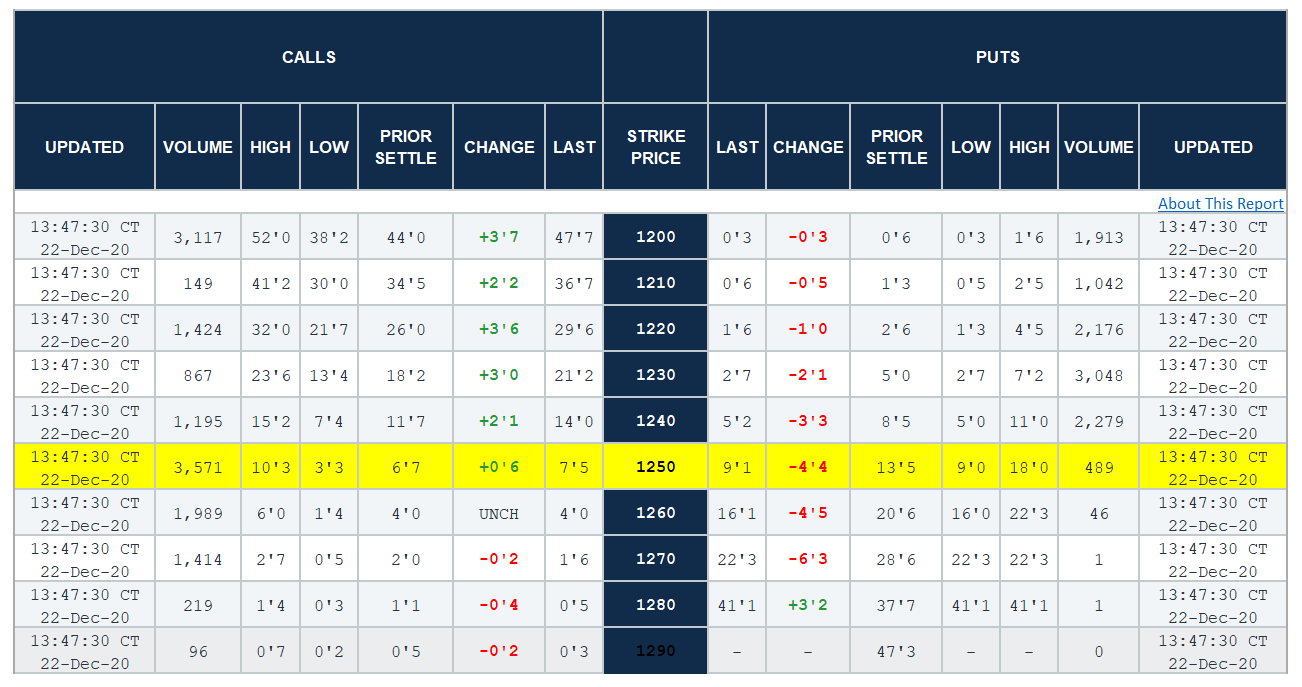
\includegraphics{assets/Options1-quotes.PNG}

}

\caption{Quotes on January 2021 Soybean Futures Options Contracts,
January Expiration}

\end{figure}%

Focus on the 1250 strike options that are highlighted in yellow. These
options contracts are also quoted in eight of a cent increments, so the
LAST price on the call option is 7'5, which means
\(7 + \frac{5}{8} = 7.625\) cents. Therefore, the cost of the 1250 call
option that expires in January is \(7.625*5000 = \$381.25\) since one
soybean contract is for 5000 bushels. That seems pretty cheap, right.
One thing to note is that the monthly options on soybean futures expire
on the last Friday at least two business days before the last business
day of the month prior to the contract month. If the Friday expiration
would land on an exchange holiday the expiration will be the business
day prior. All that means in the case of this option, it will expire on
December 24th, 2020, just two days later than the day this table was
created (notice the date updated column is for December 22, 2020). So,
while it is right at the money, there is only two trading days left in
the life of the option. What do you think happens the the value of any
given option as it gets close to expiration? We will explore in detail
in the next chapter.

Next, take a look at the LAST prices for the calls compared to the puts
as you move down the table from 1200 strikes to the 1290 strike. In the
case of the call options, the prices are increasing as you move down the
table with the largest price option being the 1200 strike. Compare that
to the put prices. The put prices are increasing as you look down the
table from the 1200 strike to the 1290 strike. Take a second and think
about why the 1200 call option is worth nearly 48 cents while the 1200
put option is worth less than half a cent.

The figure below show why: moneyness. The figure shows the call and put
with 1200 cent strike and the option premium shown in the table above.
That means that the flat part of the `hockey stick' diagram is at
-47.875 cents in the long call option figure and at -0.375 cents in the
put option figure. The 1200 strike long call is deep in the money and
has 49 cents worth of intrinsic value. The 1200 call option should be
worth a bit more than 49 cents. But sometimes the last price is a stale
price, or reflects a wide bid-ask spread in markets with inadequate
liquidity. This is often the case for deep in-the-money and deep
out-of-the-money options markets.

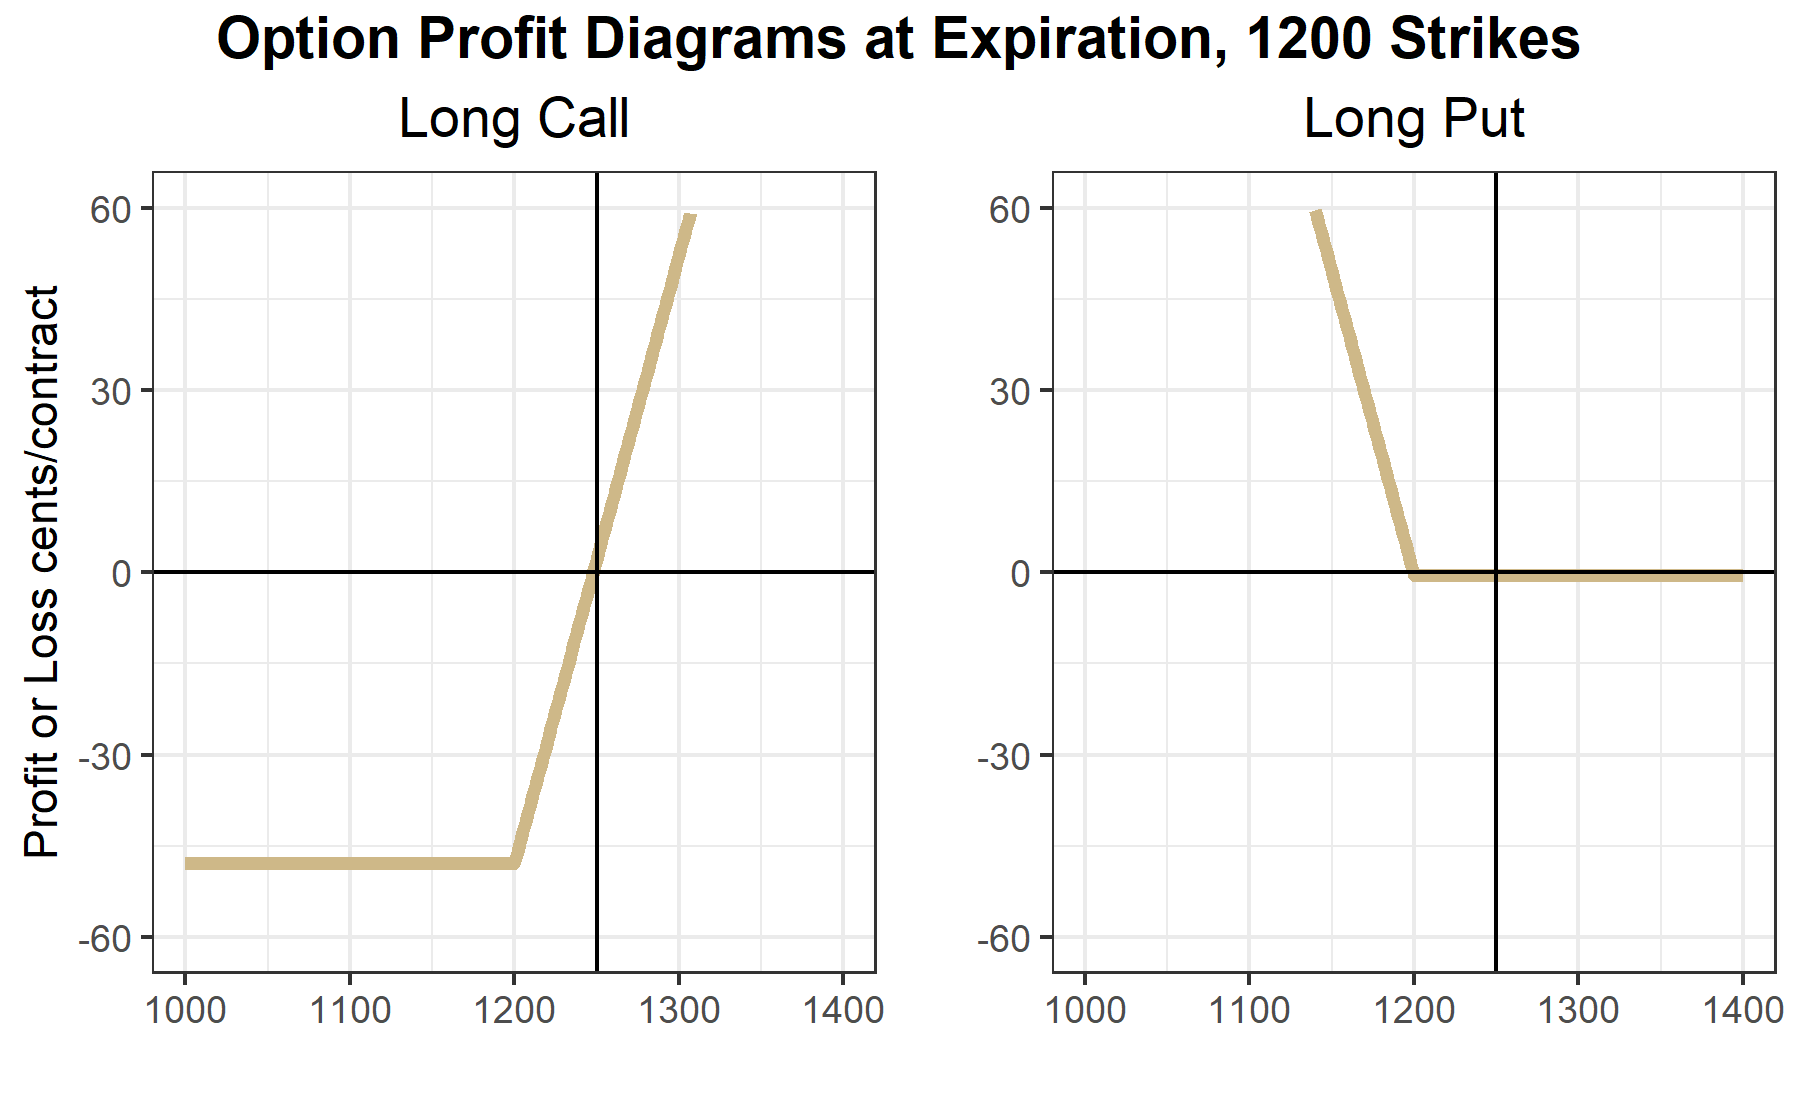
\includegraphics{assets/Options1-optionmoneynessplot.png}

Notice the volume columns for both the calls and puts compared to the
volume on the underlying. Some contracts that are near-the-money, which
means the price of the underlying is pretty close to their strike price,
have quite low volume traded. This is an example of an issue trading
option markets. Since there are so many option contracts created by
offering different strikes, liquidity gets spread thin. So if you are
trading option contracts you have to make sure the contract will be
liquid enough to get out of the position if you want to.

\section{Closing an Option Position}\label{closing-an-option-position}

There are two ways to close or `get out of' an option position: take the
opposite position or exercise (in the case of option longs) or get
exercised upon (in the case of option shorts). Taking the opposite
position is the same as exiting a position in any other familiar
instrument like a stock or futures contract. If you are long, you simply
sell the same option contract then you become `flat' or have no position
anymore. If you are short or have sold the option, you can simply buy
the same contract and become flat.

\subsection{Exercise and Assignment}\label{exercise-and-assignment}

The second way to exit the option position is to exercise (if you are
long the option) or be exercised upon (if you are short the option).
Note that you only have control over this case when you are long the
option. If you are long the option and it is in-the-money you have the
option to exercise at any time (in the case of American options which
most options trading in the United States are American). Though you
would only want to if the option is in the money. When you exercise, you
receive the corresponding position in the underlying. For example, if
you are long one call option on CME March corn futures that is
in-the-money and you exercise it, you receive a long position of one
contract in the March corn futures with your purchase price being the
strike of the option. Likewise, if you are long a put option that is
in-the-money and you exercise it you receive a short position in the
underlying at the strike price of the option. Note that if you are long
an option and you decide to exercise, you will trade a position with
zero margin requirements to having to post margin for the futures
position, because you will no longer have a position with no downside
risk.

If you are short an option contract that is in-the-money you should be
ready to be assigned (exercised upon) at any time. If a long party
indicates to the exchange that they want to exercise and you are matched
with them then you must provide them with the position in the underlying
at the strike price. For example, suppose you are short a March Corn put
with a strike of 450 cents. Price goes to 445 and you get assigned. That
means you will have a long position in the March corn futures with a
purchase price of 450. This is because as the option seller you have to
be the other side of the person who exercised their right to sell at
450.

If markets were perfect with no liquidity cost, no one should ever
exercise an option position early, since they could sell the option for
at least as much as the intrinsic value of the option. But, markets are
not perfect, and options in many markets can have wide bid-ask spreads
meaning that you will have to buy at a higher price and sell at a lower
price if you want to do the trade immediately. If the bid-ask spread is
wide enough, it may be more beneficial just to exercise and then offset
your position in the underlying.

\subsection{Option Expiration}\label{option-expiration}

Options on futures usually expire a few weeks before the underlying
futures contract expires. In most cases, the exchange will automatically
exercise in-the-money options that are held to expiration.

\bookmarksetup{startatroot}

\chapter{Advanced Option Topics}\label{advanced-option-topics}

{Interested in more? Please let me know by}
\href{https://forms.gle/Q3VByCQZHjfQSy9D7}{taking the survey}!

\textbf{Highlights}

\begin{itemize}
\item
  Black-Scholes and the Black 1976 option pricing models
\item
  Put-Call Parity and no arbitrage conditions
\item
  Implied volatility
\item
  Option Greeks
\end{itemize}

\textbf{Check your Understanding}

\begin{itemize}
\item
  How can you create a synthetic put option?
\item
  How do time to maturity and volatility impact an option's gamma?
\end{itemize}

In this chapter we will cover some more advanced concepts in options
markets. First we will learn the Black-Scholes option pricing model.
Then we will learn Put-Call Parity; we will discuss implied volatility;
then we will learn ``The Greeks'', or how option prices are impacted by
different market variables. We will learn that the Black-Scholes model
is not perfect and hear some of the most important criticisms of the
model. Lastly, we will learn the concept of delta hedging and how
options positions can be used as a hedging tool in the underlying
market.

\section{Black-Scholes Option Pricing
Model}\label{black-scholes-option-pricing-model}

The Black-Scholes option pricing model provides the price of a European
call and the price of a European put on a non-dividend paying stock. The
options we generally are focused on in the context of this book, namely
options on commodity futures on CME Group exchanges, are American
options. Since American options have all the rights of a European option
plus the right to exercise at any time, an American option cannot be
less than the price of the otherwise identical European option.
Nevertheless, this distinction is often small or zero, so the intuition
we glean from the Black-Scholes model works for the American options we
focus on in this book.

In this book we present the Black-Scholes option pricing model without
proof. Since we only provide an introduction to the concepts of option
markets a proof is beyond the scope of this book. However, there are
many well explained and free resources on the internet. The original
papers by Fischer Black, Myron Scholes and Robert Merton were published
in 1973(Black and Scholes 1973; Merton 1973). The classic text by John
Hull also provides a detailed explanation (\textbf{hull2017?}).

The most basic form of the Black-Scholes model is for options on
non-dividend paying stock. We will present this model, then we will show
the slight modification required for options on futures contracts.

\subsection{Assumptions}\label{assumptions}

First, we need to establish the assumptions required in order for the
Black-Scholes model to hold true. (\textbf{blacksc2020?})

\emph{Assumptions About Assets}

\begin{itemize}
\item
  There exists a \textbf{riskless asset} that returns a constant
  \textbf{risk free rate}
\item
  The stock price exhibits instantaneous returns that are log normal.
  More formally, the stock price follows a geometric Brownian motion and
  volatility and drift are constant. Without writing out the
  mathematical equation for the geometric Brownian motion, the drift
  term defines how much the stock price appreciates on average.
\end{itemize}

\emph{Assumptions about the Market}

\begin{itemize}
\item
  There are no arbitrage opportunities
\item
  There are no restrictions on borrowing and lending at the risk free
  rate
\item
  Market participants can buy or sell unlimited quantities of the stock
\item
  There are no transactions costs
\end{itemize}

\subsection{Notation}\label{notation}

\begin{itemize}
\item
  \(C\) = Call Option Price
\item
  \(P\) = Put Option Price
\item
  \(S\) = Current Stock Price
\item
  \(K\) = Strike Price
\item
  \(r\) = Risk free rate
\item
  \(\sigma\) = Standard deviation of the stock price returns
\item
  \(t\) = Time to maturity (in fraction of a year)
\item
  \(N\) = Standard normal cumulative distribution function
\item
  \(d_{1} = \frac{ln(\frac{S_{t}}{K}) + (r + \frac{\sigma^{2}}{2})t}{\sigma \sqrt{t}}\)
\item
  \(d_{2} = d_{1} - \sigma \sqrt{t}\)
\end{itemize}

The formula for a call option on a non-dividend paying stock with strike
price \(K\) that has time to maturity \(t\) is:

\[C = S_{t}N(d_{1}) - K e^{-rt} N(d_{2})\]

The price of a similar put option is:

\[
P = N(-d_{2}) K e^{-rt} - N(-d_{1}) S_{t}
\]

\subsection{Option Pricing Formula for Futures
Contracts}\label{option-pricing-formula-for-futures-contracts}

Black (1976) derives a version of the Black-Scholes model that is
appropriate for pricing futures contracts. The key difference between
the two option pricing models is that stock trading requires that the
full value of the stock be spent upfront. Thus, the \(S_{t}\) in the
Black-Scholes equations above is referencing expenditures at the current
time, and do not need to be discounted. Futures contracts differ in that
entering into a futures contract does not require expenditure upfront
(besides posting margin). Therefore, the price of the underlying should
be discounted, bringing the future value of the expenditure related to
the futures contract to the present. The Black equations for pricing
call and put options on commodity futures are therefore as follows:

\[
C = F_{t} e^{-rt} N(d_{1}) - K e^{-rt} N(d_{2})
\]

and

\[
P = N(-d_{2}) K e^{-rt} - N(-d_{1}) F_{t} e^{-rt}
\]

\section{Put-Call Parity}\label{put-call-parity}

Put and call options of the same strike price and same expiration have
to follow a specific relationship. That means that if you know the price
of a call option, the price of the put option with the same strike and
expiration is determined or there is an arbitrage opportunity.

To illustrate why this must be true consider the example below in the
embedded Google Sheets file. The cells in gold are editable so that you
can play around with the put-call parity result. The default values are
shown in row 3, replace the default values if the values in gold do not
match the defaults. If you would rather work with the full size Google
sheet you can find it at
\href{https://docs.google.com/spreadsheets/d/1ivvTGqC9R4L3zkG8c4ApDg8dC1LHj4v_8uLjgiurxX0/edit?usp=sharing}{Put-Call
Parity Sheet}.

Suppose that the price of the underlying is 470 cents, and a call option
with strike price of 450 cents has a premium of 25 cents. In the table
we consider underlying price ranges from 400 to 500 cents. Then we
calculate the profit at expiration from the call option in the second
column of the table. From 400 cents to 450 cents the profit would be -25
cents. Then as the price of the underlying increases from 450 to 500
cents the profit of the call option at expiration increases one for one.
Clicking in \texttt{B7} shows the formula for the call option profit at
expiration to be \texttt{=max(0-\$B\$2,\ A7-\$C\$2-\$B2}. In the plot
the call option profit is the `hockey stick' shaped line in black.

In the third column we have the profit from a short position in the
underlying futures contract where the position was initiated at the
current price of the underlying (470 cents). Clicking in \texttt{C7}
shows the formula for the profit of this position is
\texttt{=\$D\$2-A7}. Being a short position, this position makes money
as the price of the underlying falls. This position is shown by the
straight black line that crosses the x-axis at 470 in the figure.

The fourth column shows what your profit at expiration would look like
if you bought the call option and also sold the underlying futures for
470. Clicking on \texttt{D7} shows that the formula for this payoff is
simply \texttt{=B7+C7}, or the sum of the profit in each position. This
profit function is shown in gold.

Notice that the gold line looks exactly like the profit at expiration of
a put option with strike equal to 450 cents! This is called a synthetic
put position. So, it must be that the put option premium in this example
is 5 cents, otherwise you could buy the synthetic and sell the real put
or vice versa and make a riskless profit. This relationship between the
call and put price is called put-call parity.

Take a minute and play around with different values of call option
premium. For example, try 50, 30, and 10. What is strange about premium
= 10 cents?

As an aside, note that you can create a synthetic call option by buying
a put option and buying the underlying.

\section{Implied Volatility}\label{implied-volatility}

Notice that of all the variables that go into the option pricing model,
the only ones we don't know beforehand are the option price and
\(\sigma\) (the standard deviation of returns of the underlying). That
means if we plug in all the numbers we know into the option pricing
formula and then make a guess, or a good estimate of what \(\sigma\)
should be the formula will give us an estimate of what the option should
be worth as well.

In practice we usually do the opposite because we can observe the
markets where these options are trading and know what prices the option
is being bought and sold for at any moment the markets are open. If
instead we take these prices that are actually trading in the market and
use that in the formula, then we can solve for \(\sigma\) and we get a
measure of the volatility `implied' by the prices at which the option is
currently trading for.

Implied volatility is an important measure because it tells you how much
of a move traders expect the underlying could make. Implied volatility
is normalized to units of \% per annum so that you might see and implied
volatility of 16\% which means that option market participants think the
underlying could move (in either direction) 16\% per
year(\textbf{ganti?}). The implied volatility is always changing though.
In fact, that is one criticism of the Black-Scholes model. The model
requires the underlying to have constant volatility, which is clearly
not the case for any asset.

In the next sections we will explore how the different variables in the
option pricing model affect option prices. We will see that implied
volatility has a big impact. High implied volatility means high option
prices all else equal.

\section{Option Prices Compared to the Profit
Diagram}\label{option-prices-compared-to-the-profit-diagram}

In the Google Sheet embedded below we have plotted in gold the price of
a call and put option with strike price of 450 cents along with the
intrinsic value of the option plotted in black. Remember that the
intrinsic value of the option is what the option is worth at expiration
given the value of the underlying, not considering the premium paid.
Therefore, if we take the profit diagrams we considered from the
previous chapter and moved the flat part of the hockey stick diagram to
the x-axis we get the intrinsic value of the option.

Notice a few things about the option price line. First of all, for every
value of the underlying the call price is above the black line. That is
because the price of an option prior to expiration must be worth at
least as much as its intrinsic value, with a little bit extra to account
for the uncertainty in price that could change the moneyness of the
option before it expires.

Further, notice that the option differs from its intrinsic value most
near the strike price; this is because the option price must smooth out
the kink in the intrinsic value diagram.

\section{Option Greeks}\label{option-greeks}

In this section we will learn the option `greeks'. This, along with the
second derivatives, will do more than anything to give you a better
understanding of how option prices really work. As you read this section
keep looking back to the embedded plot of option prices in section
@ref(option-prices-compared-to-the-profit-diagram)

\textbf{Delta}

The delta of a call option is \(\Delta = \frac{\partial C}{\partial F}\)
, and the delta of a put option is
\(\Delta = \frac{\partial P}{\partial F}\), or how much the value of a
call option changes as the underlying changes. Literally, this is the
slope of the line representing the option price. The main thing is to
notice that as the price of the underlying moves larger the call option
is more in the money, and the delta of the call option approaches +1. As
the price of the underlying moves larger the put option moves more out
of the money and the delta of the put option approaches 0. As the price
of the underlying moves lower, the delta of the call option approaches 0
and the delta of the put option approaches -1. Also, notice that at the
money, the delta of the call option is +0.5 and the delta of the at the
money put option is -0.5.

\textbf{Gamma}

The gamma of a call option is
\(\gamma = \frac{\partial^2 C}{\partial F^2}\) and the gamma of a put
option is \(\gamma = \frac{\partial^2 P}{\partial F^2}\), that is it
tells you the curvature of the option price with respect to the
underlying. Which is to say, how much additional \(\Delta\) do you get
as the underlying price increases. Looking above at the price of the
call option, notice that at an underlying price of 425 the option line
is pretty flat (low delta), while at an underlying price of 475 the
option line is pretty steep and nearly equal to the slope of the black
line which is 1. The curvature in the line that is required to get from
a flat slope to a steep slope is the \(\gamma\) of the option.

An option's \(\gamma\) is the friend of speculators who use options.
Large \(\gamma\) allows a trader to buy a cheap out of the money option
on an underlying they know will move up or down. If they are right their
position enjoys convex gains. The higher the \(\gamma\) the better it is
for the directional speculator using long option positions. However, we
will see that \(\gamma\) is counter-balanced by the next greeks we will
learn.

\textbf{Theta}

Option's lose value as expiration nears due to reduced uncertainty
related to where the price of the underlying will be relative to the
strike. This `time decay' is made explicit by the theta of the option.
Theta of a call option is \(\theta = \frac{\partial C}{\partial t}\) and
the theta of a put option is \(\theta = \frac{\partial P}{\partial t}\).
Theta is how option sellers make money and theta is the enemy of long
option holders. Theta is usually quoted in terms of how much the option
will lose value per day, all other things equal. Go back to the embedded
Google Sheet in @ref(option-prices-compared-to-the-profit-diagram). Play
around with the time value in the option premium by putting in some
larger and smaller values for time to maturity. Remember, the units of
time to maturity is fraction of a year. So if you put in 0.5 that is the
same as six months, and 0.02 is about one week.

For reference, focus on the at-the-money call and put options with
strike of 450. With time to maturity = 0.5, the call option is worth
19.89 cents (or 4.4\% of the value of the underlying contract) while the
put option is worth 28.89 cents (6.4\% of the value of the underlying
contract). With time to maturity = 0.02, the call option is worth 4.06
cents (0.90\% of the value of the underlying contract) and the put
option is worth 4.42 cents (0.98\% of the value of the underlying
contract).

Another thing to notice is how the pace of theta decay accelerates as
time to maturity approaches. Try setting the time to maturity cell (E2)
to \texttt{=180/365} then to \texttt{=173/365} and notice how much the
gold lines of the option prices shift down. Compare that to how much the
gold lines shift down when you do \texttt{=10/365} and \texttt{=3/365}.
In both cases one week passed between the first and second time
calculated, but the option lost a lot more value both nominally and in
percentage terms in the second case.

\textbf{Vega}

Vega measures sensitivity of the option value to changes in the
volatility. In other words, Vega
\(= \frac{\partial C}{\partial \sigma}\) in the case of call options and
Vega = \(= \frac{\partial P}{\partial \sigma}\) in the case of put
options. An increase in volatility will cause an increase in options
prices, all other things equal. Play with different values in
@ref(option-prices-compared-to-the-profit-diagram) try volatility as low
as 10 and as high as 100. Also, see what impact changes in volatility
has for different time to maturity values.

\textbf{Other Greeks}

There are other greeks (including Rho, Vanna, Vomma, and more) that
become important if you are involved in managing a large book of options
positions, but we will not cover them in detail. The
\href{https://en.wikipedia.org/wiki/Greeks_(finance)}{Greeks Wikipedia
page} is a good place to start if you are interested.

\textbf{How other Volatility and Time-to-Maturity Impacts Gamma}

For a couple of the greeks we mentioned how they interact with each
other, or react to different times to maturity. Here I just want to
point out a bit more about this mechanics. I mentioned that \(\gamma\)
is the friend of the option buyer and it is the foe of the option seller
because of the convex shape of the return profile you get with large
gamma.

So what makes \(\gamma\) large? Biggest things giving large \(\gamma\)
would be short time to maturity and low volatility. However, both of
these have drawbacks for the option buyer. When time to maturity is
short, \(\theta\) decay is fast, which works against the option buyer.
Regarding volatility, sure low volatility produces large gamma, but
option buyers get the most benefit from gamma by buying slightly out of
the money options prior to a significant move in their favor. Thus,
periods of low volatility make a significant move less likely.

So even though the option buyer can create countless profit scenarios
over many price ranges, at the end of the day, profitable option buying
for speculation requires anticipating a significant price move to pay
off.

\section{Criticisms of the Black-Scholes Pricing
Model}\label{criticisms-of-the-black-scholes-pricing-model}

We should be aware that while the Black-Scholes option pricing model is
very elegant and easy to work with, it has some limitations. Most
limitations stem from unrealistic assumptions underpinning the model.

Recall the model assumptions from earlier:

\begin{quote}
\emph{Assumptions About Assets}

\begin{itemize}
\item
  There exists a riskless asset that returns a constant risk free rate
\item
  The stock price exhibits instantaneous returns that are log normal.
  More formally, the stock price follows a geometric Brownian motion and
  volatility and drift are constant. Without writing out the
  mathematical equation for the geometric Brownian motion, the drift
  term defines how much the stock price appreciates on average.
\end{itemize}

\emph{Assumptions about the Market}

\begin{itemize}
\item
  There are no arbitrage opportunities
\item
  There are no restrictions on borrowing and lending at the risk free
  rate
\item
  Market participants can buy or sell unlimited quantities of the stock
\item
  There are no transactions costs
\end{itemize}
\end{quote}

These assumptions are at odds with several commonly observed attributes
of real markets . In particular, assets commonly have the following
characteristics:

\begin{enumerate}
\def\labelenumi{\arabic{enumi}.}
\tightlist
\item
  Heavy-tailed returns
\item
  Positively correlated volatility, volatility clustering, variable
  volatility
\end{enumerate}

The first item means that extreme market movements (up or down) happen
more often than implied by the normal distribution. Since option prices
depend on the full probability distribution of potential outcomes, a
model that assumes a normal distribution will chronically under-price
options.

The second item reflects the tendency in markets for volatility events
to be clustered together. That means if we have a large price movement,
it will likely be followed by large price movements in the near future.
We cannot predict whether it will be up or down, but we can be sure it
will be volatile. In the figure below we plot continuous series of
weekly soybean futures since 2010 in the first panel. In the second
panel we plot squared log differences of prices, which is one way to
calculate volatility. You can clearly observe the positive correlation
and volatility clustering in this market. Once there is an event that
spikes volatility, it takes a while for volatility to `calm down'.

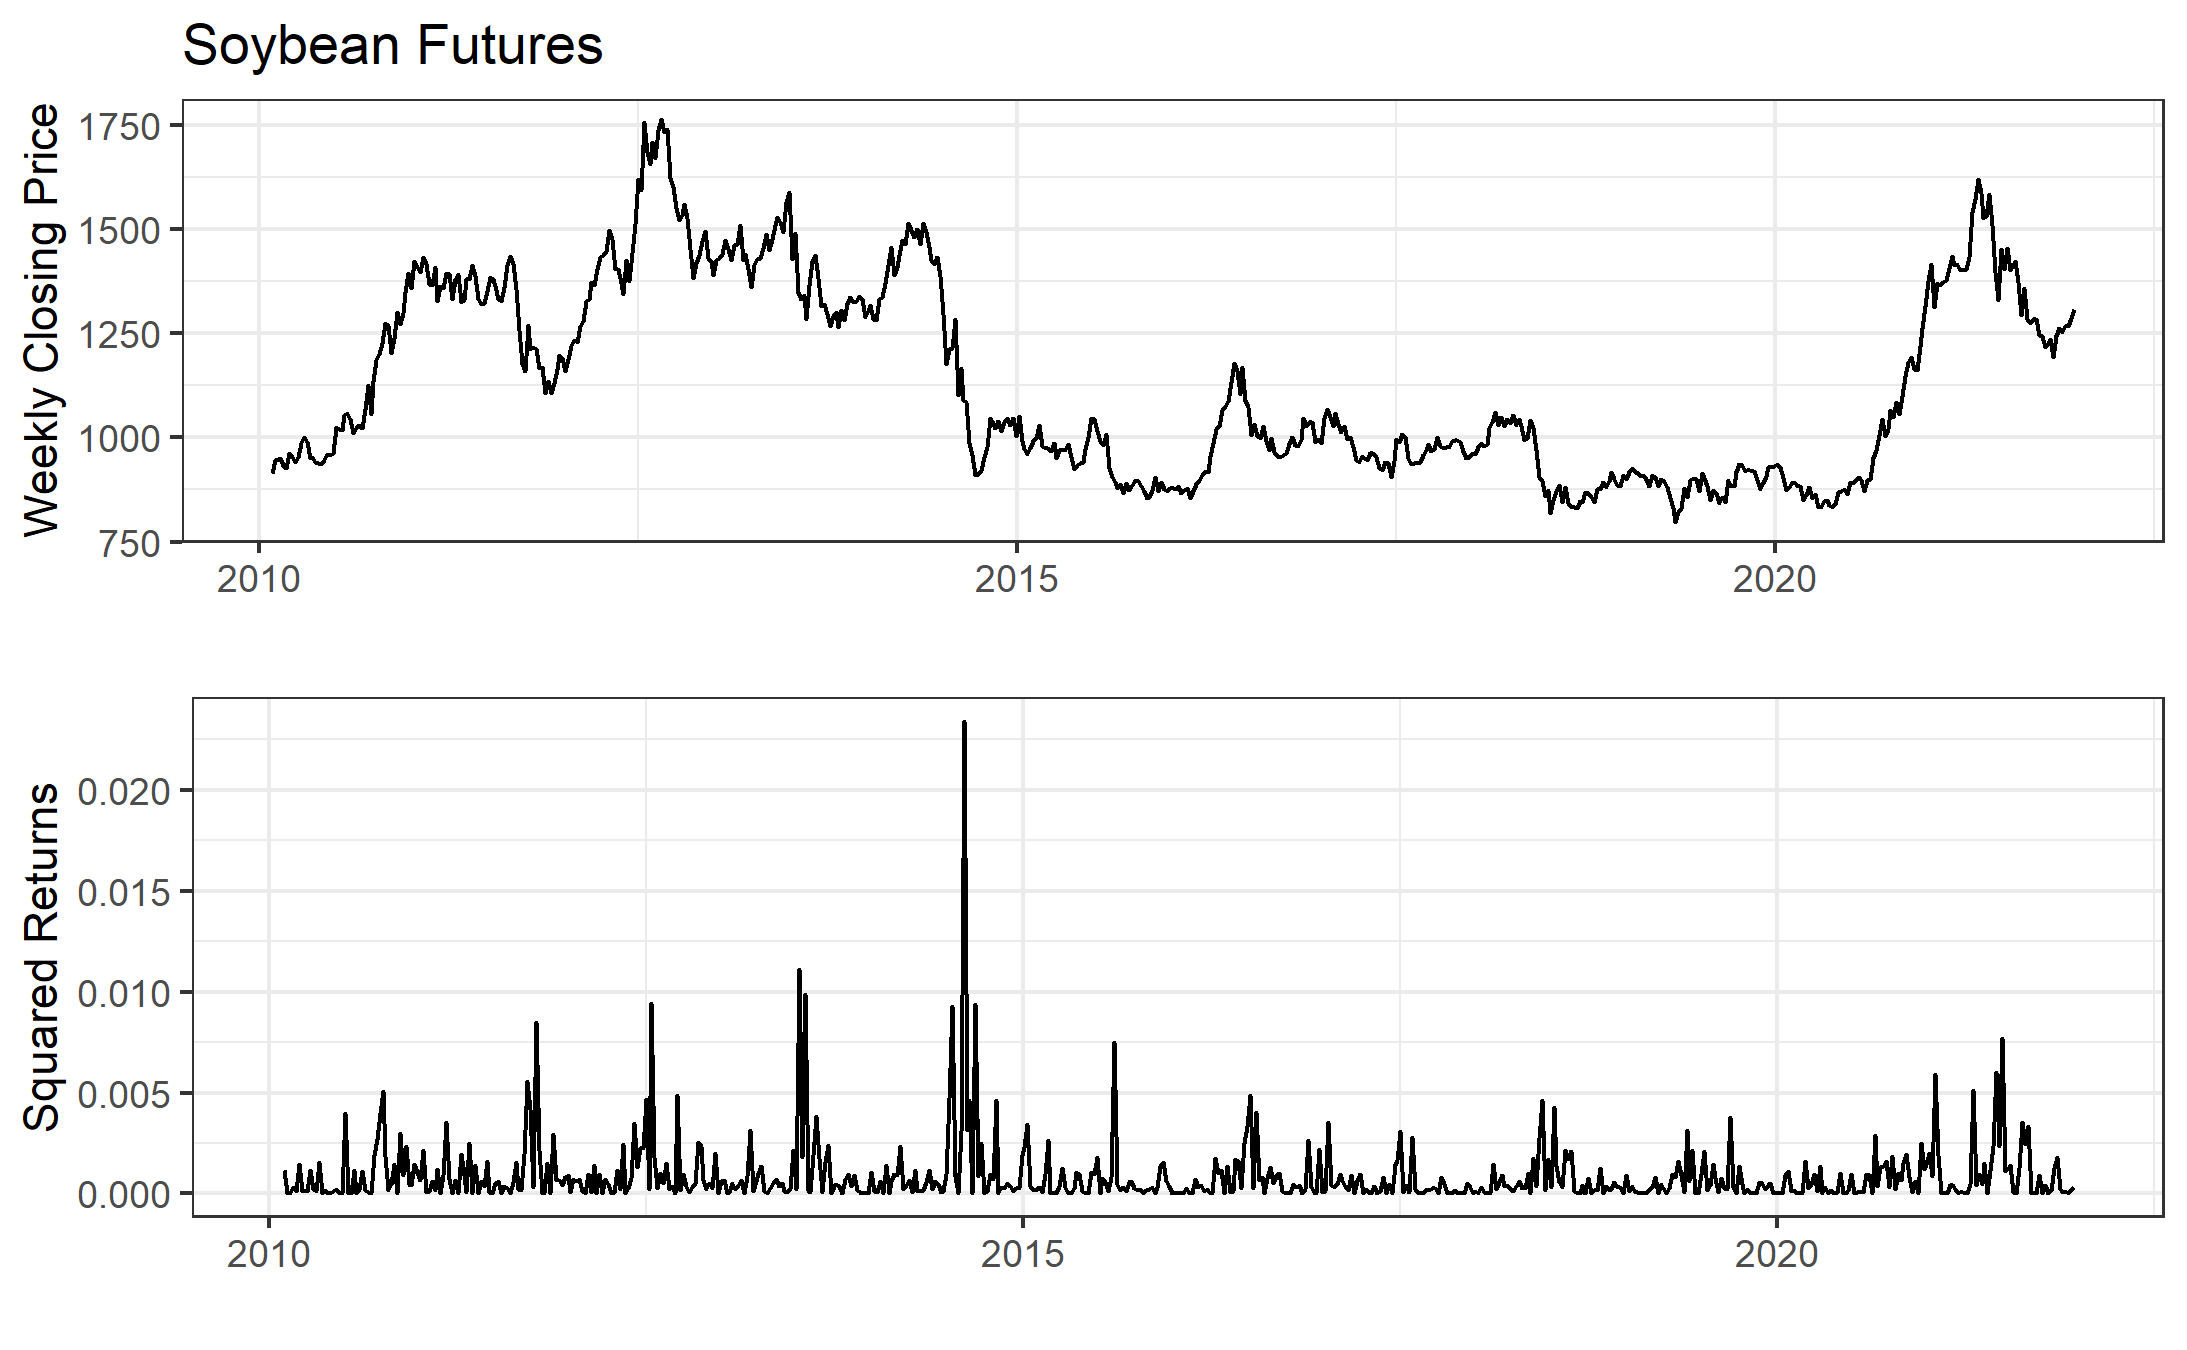
\includegraphics{assets/Options2-volcluster.png}

This explains the limitation of the Black-Scholes model along the
volatility dimension. Another practical matter is that the model
requires one to continuously maintain a perfectly hedged portfolio of an
option and the underlying asset. This can be impossible when prices
experience `jumps' or non continuous movements. These can occur in due
to unexpected information hitting the market and traders pulling their
standing orders in the market. But, it also occurs during routine market
closures. The overnight jumps can be substantial in cases where a lot of
information is revealed overnight.

\section{Delta Hedging}\label{delta-hedging}

One proof of the Black-Scholes option pricing formula shows that if one
can continuously hedge the sale of an option contract with the
underlying asset so that the position is `delta neutral' then the hedged
portfolio (the short option and long stock) is riskless and therefore
must earn the `risk-free rate'. This implies that if you know the price
of the stock and you know the risk free rate, then you can deduce what
the price of the option should be at any time. Solving that yields the
Black-Scholes equation.

Let's discuss the delta neutral concept more fully. Recall that the
\(\Delta\) (delta) of an option is
\(\Delta = \frac{\partial C}{\partial F}\), or how much the price of the
option changes if the price of the underlying asset increases by one
unit. A position is said to be `delta neutral' if options and the
underlying asset are held in a proportion such that for small changes in
the underlying asset's price, the value of the position is unchanged.

\textbf{Example}

Suppose the price of the nearby corn futures contract is 450 cents. A
trader might sell 100 the 450 strike call options that are trading for
11 cents. The trader is hoping to profit from theta decay, as the price
of the option decreases over time. They do not want exposure to the
changing price of the futures contract, however.

\begin{enumerate}
\def\labelenumi{\arabic{enumi}.}
\tightlist
\item
  How many futures contracts should they buy/sell to make their position
  delta neutral?
\end{enumerate}

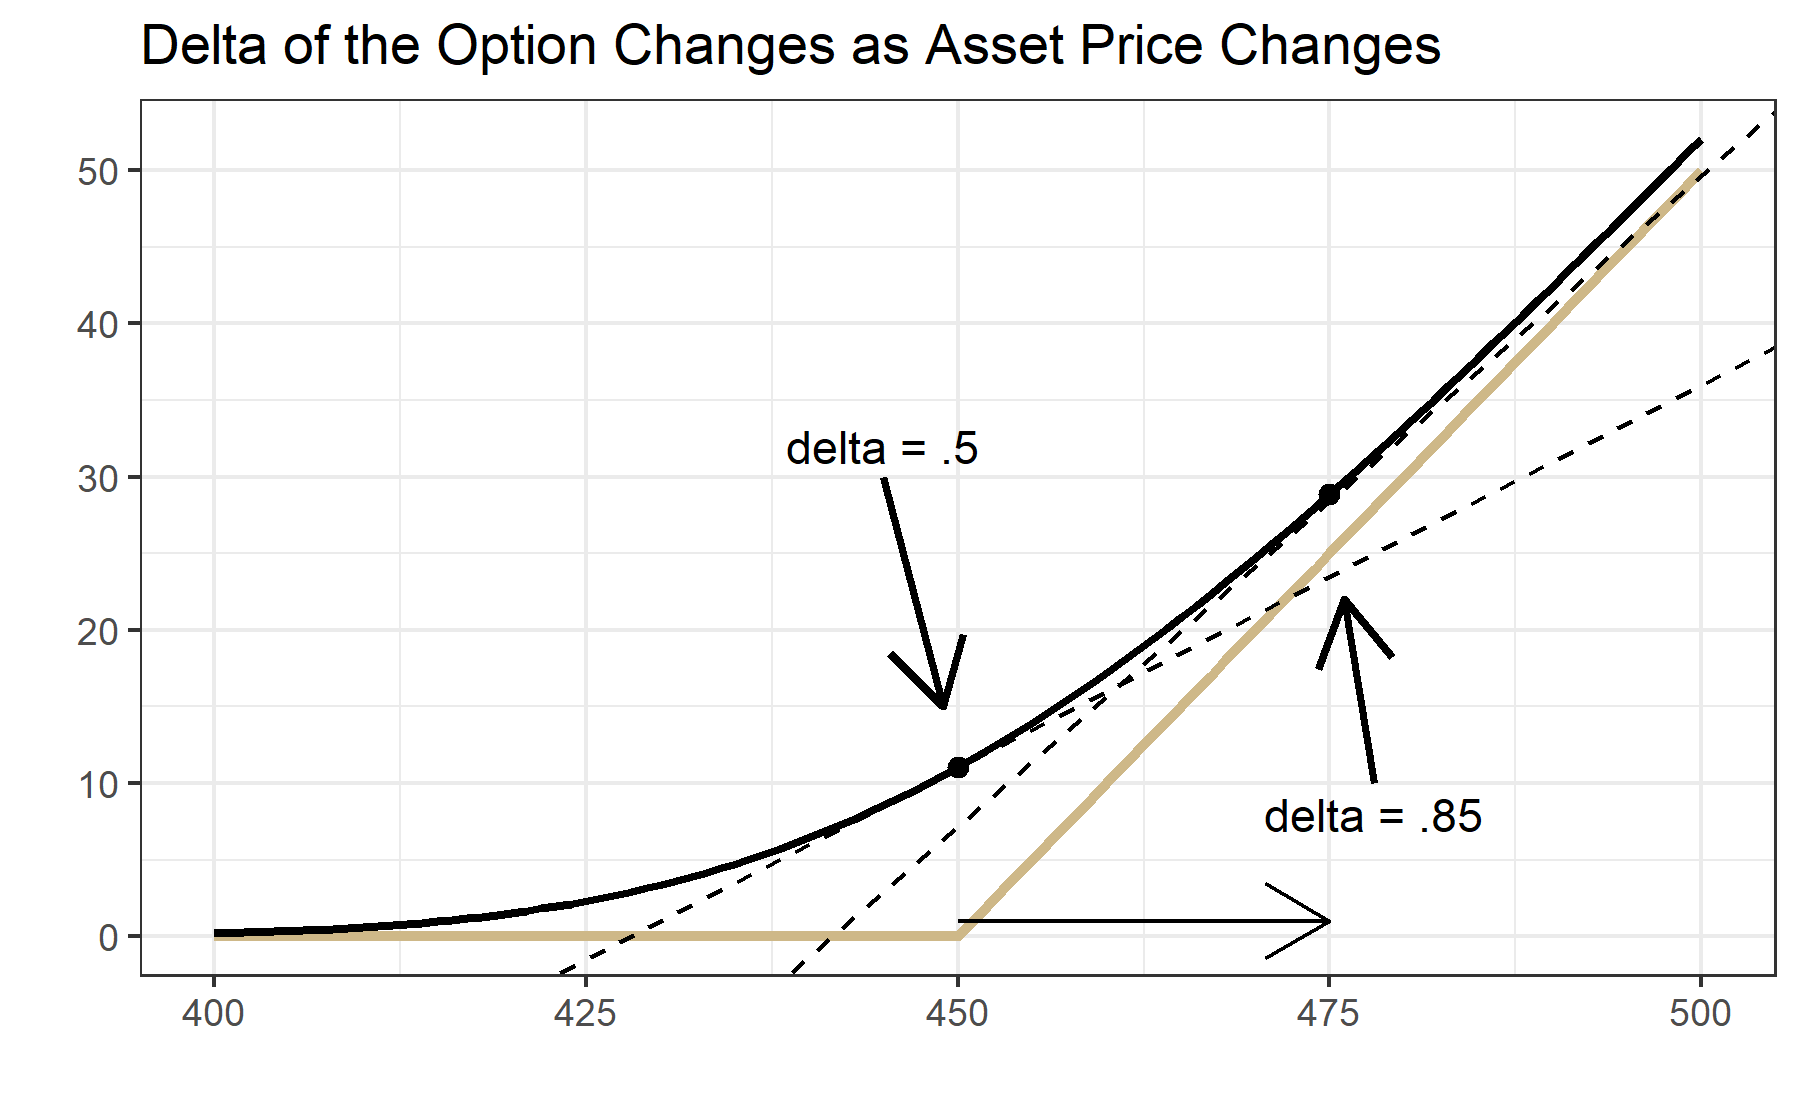
\includegraphics{assets/Options2-deltahedge.png}

\textbf{Answer}: Consider the figure above. The gold `hockey stick' line
represents the payoff of the call option to someone long the option. The
thick black line is the Black-Scholes price of the option at the current
time, for different values of the underlying (indicated on the x-axis).
The dashed black lines show that at 450, the slope of the option price
curve is .5 and at 475 the slope is .85. These are the delta's of the
option price when the underlying is 450 and 475, respectively.

Since the \(\Delta\) of the 450 strike option is 0.5 that means that the
price of the option increases (decreases) by .5 times the futures price
increase (decrease). Another way to think about it is selling the 100 of
the 450 strike call options is like being short 50 of the futures; with
a delta of .5 every 1 cent change in the underlying results in a .5 cent
change in the option. So, if the trader does not want price exposure,
they can \textbf{buy} 50 futures contracts at the same time they
\textbf{sell} the call options. Now, for small changes in the futures
price around 450, they are fully hedged.

As an example consider what happens to their delta-hedged position for a
modest price increase of 2 cents in the futures contract from 450 to
452. This will imply the call option increases to 12.18 cents, all else
being equal. Walking through the profit an loss calculations in this
case, we see the trader loses \$600 from this price movement. Recall,
they are short the premium of \$55,000 that they are hoping to pocket as
time eats away at the premium. They do experience a loss from this, but
it will likely be outweighed by the premium decay if the price does not
continue to rise too fast.

\begin{longtable}[]{@{}
  >{\raggedright\arraybackslash}p{(\columnwidth - 4\tabcolsep) * \real{0.2472}}
  >{\raggedright\arraybackslash}p{(\columnwidth - 4\tabcolsep) * \real{0.3483}}
  >{\raggedright\arraybackslash}p{(\columnwidth - 4\tabcolsep) * \real{0.3933}}@{}}
\caption{Change in value of delta-hedged position after small price
move}\tabularnewline
\toprule\noalign{}
\begin{minipage}[b]{\linewidth}\raggedright
\end{minipage} & \begin{minipage}[b]{\linewidth}\raggedright
Short Calls
\end{minipage} & \begin{minipage}[b]{\linewidth}\raggedright
Long Futures
\end{minipage} \\
\midrule\noalign{}
\endfirsthead
\toprule\noalign{}
\begin{minipage}[b]{\linewidth}\raggedright
\end{minipage} & \begin{minipage}[b]{\linewidth}\raggedright
Short Calls
\end{minipage} & \begin{minipage}[b]{\linewidth}\raggedright
Long Futures
\end{minipage} \\
\midrule\noalign{}
\endhead
\bottomrule\noalign{}
\endlastfoot
t = 0 & & \\
Price & 11.06 cents per contract & 450 \\
Quantity & 100 contracts & 50 \\
\textbf{Value} & (11.06/100)*100*5000 =

\textbf{\$55,300} & (450/100)*50*5000 =

\textbf{\$1,125,000} (notional value) \\
t = 1 & & \\
Price & 12.18 cents per contract & 452 \\
Quantity & 100 & 50 \\
\textbf{Value} & (12.18/100)*100*5000 =

\textbf{\$60,900} & (452/100)*50*5000 =

\textbf{\$1,130,000} (notional value) \\
\textbf{Profit/Loss} & 55,300 - 60,900 =

\textbf{-\$5,600} & 1,130,000 - 1,125,000 =

\textbf{+\$5,000} \\
\textbf{Net Profit/Loss} & 62,500 - 89,000 = \textbf{-\$600} & \\
\end{longtable}

\begin{enumerate}
\def\labelenumi{\arabic{enumi}.}
\setcounter{enumi}{1}
\tightlist
\item
  Suppose now that the futures price experiences a big increase to 475
  from close of the day session to open of the night session. Is the
  trader's position still delta neutral? What should they do to get
  their position delta neutral?
\end{enumerate}

\textbf{Answer}:

To recap, our trader is short 100 of the 450 call options and bought 50
futures contracts against it when the futures price was 450 to get their
position delta neutral. Then the price of the futures contract went to
475 between the close of the day session and open of the night session,
so they could not adjust their hedge gradually. The price `jumped' to
475. That means that the option position now has a delta of -.85*100
(negative because our trader is short the option) and only has +1*50
delta from the long futures position (the outright futures position
always had a delta of 1). To get delta neutral the trader needs to buy
an additional 35 futures contracts to get the delta of their futures
position to +1*.85, but doing so does not erase the loss they
experienced from the rise in price from 450 to 475, it just gets them
delta-hedged against small price movements going forward.

\subsection{Why is delta-hedging not
fool-proof?}\label{why-is-delta-hedging-not-fool-proof}

Delta hedging only works if traders can continuously re-balance their
option and futures positions to keep delta neutral as prices change.
There are a couple major problems with this.

First is that it is costly to re-balance. Traders face trading costs
from commissions, fees, and/or the bid-ask spread. Re-balancing too
often would quickly eat into whatever profit they hoped to earn from
theta-decay.

Second, sometimes market prices move in significant `jumps'. Whether
this comes from information hitting the market that causes resting
orders on the order book to be canceled and resent at much higher (or
lower) prices, or from prices changing significantly from the market
close to open, the result is the same for the delta neutral trader. They
will have to re-balance their position after a large discrete jump. If
the price jump goes against them, they will lock in a loss.

In our example above, if the move from 450 to 475 happens from between
market close and the next market open, the traders position will have a
bigger loss on the short call option position than gain in the long
futures position, due to the significant change in slope (or delta) of
the option price.

\begin{longtable}[]{@{}
  >{\raggedright\arraybackslash}p{(\columnwidth - 4\tabcolsep) * \real{0.2391}}
  >{\raggedright\arraybackslash}p{(\columnwidth - 4\tabcolsep) * \real{0.3696}}
  >{\raggedright\arraybackslash}p{(\columnwidth - 4\tabcolsep) * \real{0.3804}}@{}}
\caption{Change in value of delta-hedged position after big price
move}\tabularnewline
\toprule\noalign{}
\begin{minipage}[b]{\linewidth}\raggedright
\end{minipage} & \begin{minipage}[b]{\linewidth}\raggedright
Short Calls
\end{minipage} & \begin{minipage}[b]{\linewidth}\raggedright
Long Futures
\end{minipage} \\
\midrule\noalign{}
\endfirsthead
\toprule\noalign{}
\begin{minipage}[b]{\linewidth}\raggedright
\end{minipage} & \begin{minipage}[b]{\linewidth}\raggedright
Short Calls
\end{minipage} & \begin{minipage}[b]{\linewidth}\raggedright
Long Futures
\end{minipage} \\
\midrule\noalign{}
\endhead
\bottomrule\noalign{}
\endlastfoot
t = 0 & & \\
Price & 11.06 cents per contract & 450 \\
Quantity & 100 contracts & 50 \\
\textbf{Value} & (11.06/100)*100*5000 =

\textbf{\$55,300} & (450/100)*50*5000 =

\textbf{\$1,125,000} (notional value) \\
t = 1 & & \\
Price & 28.86 cents per contract & 475 \\
Quantity & 100 & 50 \\
\textbf{Value} & (28.86/100)*100*5000 =

\textbf{\$144,300} & (475/100)*50*5000 =

\textbf{\$1,187,500} (notional value) \\
\textbf{Profit/Loss} & 55,300 - 144,300 =

\textbf{-\$89,000} & 1,187,500 - 1,125,000 =

\textbf{+\$62,500} \\
\textbf{Net Profit/Loss} & 62,500 - 89,000 = \textbf{-\$26,000} & \\
\end{longtable}

\subsection{Famous Blow-Ups in Delta-Hedging
Operations}\label{famous-blow-ups-in-delta-hedging-operations}

Large unexpected price movements, have a storied history of blowing up
hedge funds who focus on selling volatility. Several articles are linked
below for the interested reader.

\begin{enumerate}
\def\labelenumi{\arabic{enumi}.}
\tightlist
\item
  \href{https://volquant.medium.com/epic-failures-lessons-from-volatility-funds-blow-ups-6f4226c8334f}{``Epic
  Failures - Lessons from Volatility Funds Blow-Ups.'' Harel Jacobson}
\item
  \href{https://www.ft.com/content/b8ddbf92-c9b4-4a81-a167-ef9ee80962a5}{``Turbulent
  Markets Upend Volatility Hedge Funds.'' Laurence Fletcher and Richard
  Hendarson, FT.}
\item
  \href{https://www.institutionalinvestor.com/article/b1m6kkzscgqrl0/How-to-Lose-a-Billion-Dollars-Without-Really-Trying}{``How
  to Lose a Billion Dollars Without Really Trying.'' Leanna Orr.
  Institutional Investor.}
\end{enumerate}

\begin{quote}
History doesn't repeat itself, but it often rhymes. --- Mark Twain
\end{quote}

\begin{quote}
Its like picking up pennies in front of a steamroller. --- Unknown
\end{quote}

These stories have a common theme. A fund engages in a strategy of
selling volatility (selling calls, selling puts, selling vix futures,
etc) with high leverage. The high leverage and nature of volatility
premium mean these funds make spectacular returns for as long as there
is not a `volatility event'. One day, the volatility event arrives and
anyone with a highly leveraged short volatility position is highly
likely to blow up (total loss of trading capital).

\bookmarksetup{startatroot}

\chapter{Hedging with Options}\label{hedging-with-options}

{Interested in more? Please let me know by}
\href{https://forms.gle/Q3VByCQZHjfQSy9D7}{taking the survey}!

\textbf{Highlights}

\begin{itemize}
\tightlist
\item
  Hedge a speculative position with options
\item
  Put options can be used to hedge a farmers production risk
\item
  Hedging with options is costly
\item
  Farmer's hedge; putting on a fence
\end{itemize}

\textbf{Check Your Understanding}

\begin{itemize}
\tightlist
\item
  Why does a long put option protect from downside risk?
\item
  What are the options trades required to lock in a price range?
\item
  Which of the strategies described in this chapter require one to
  maintain margin?
\end{itemize}

\section{Farmer Hedging Price Risk on Production with a Put
Option}\label{farmer-hedging-price-risk-on-production-with-a-put-option}

We know from chapter 4 that hedging in the financial sense is an
activity designed to generate positive cash flows when the main pain
position is experiencing a drawdown. The classic example being a farmer
who has a crop in the field or in the bin is exposed to price risk and
will experience financial loss if crop prices decline. To hedge this
risk, they can sell a futures contract. Corn futures prices are highly
correlated to the spot price the farmer faces in the local market. So if
corn prices decline, the losses in spot sales are offset by gains from
the short futures position.

Hedging with futures has the disadvantage of removing exposure to both
downside \emph{and} upside price movements. By hedging with a put
option, a farmer can eliminate downside risk (save for the risk of a
falling basis) while retaining benefits from price increases.

To visualize how it works first recall what a farmer's per bushel
revenue looks like as a function of the price of corn. Its simply a 45
degree line radiating from the origin.

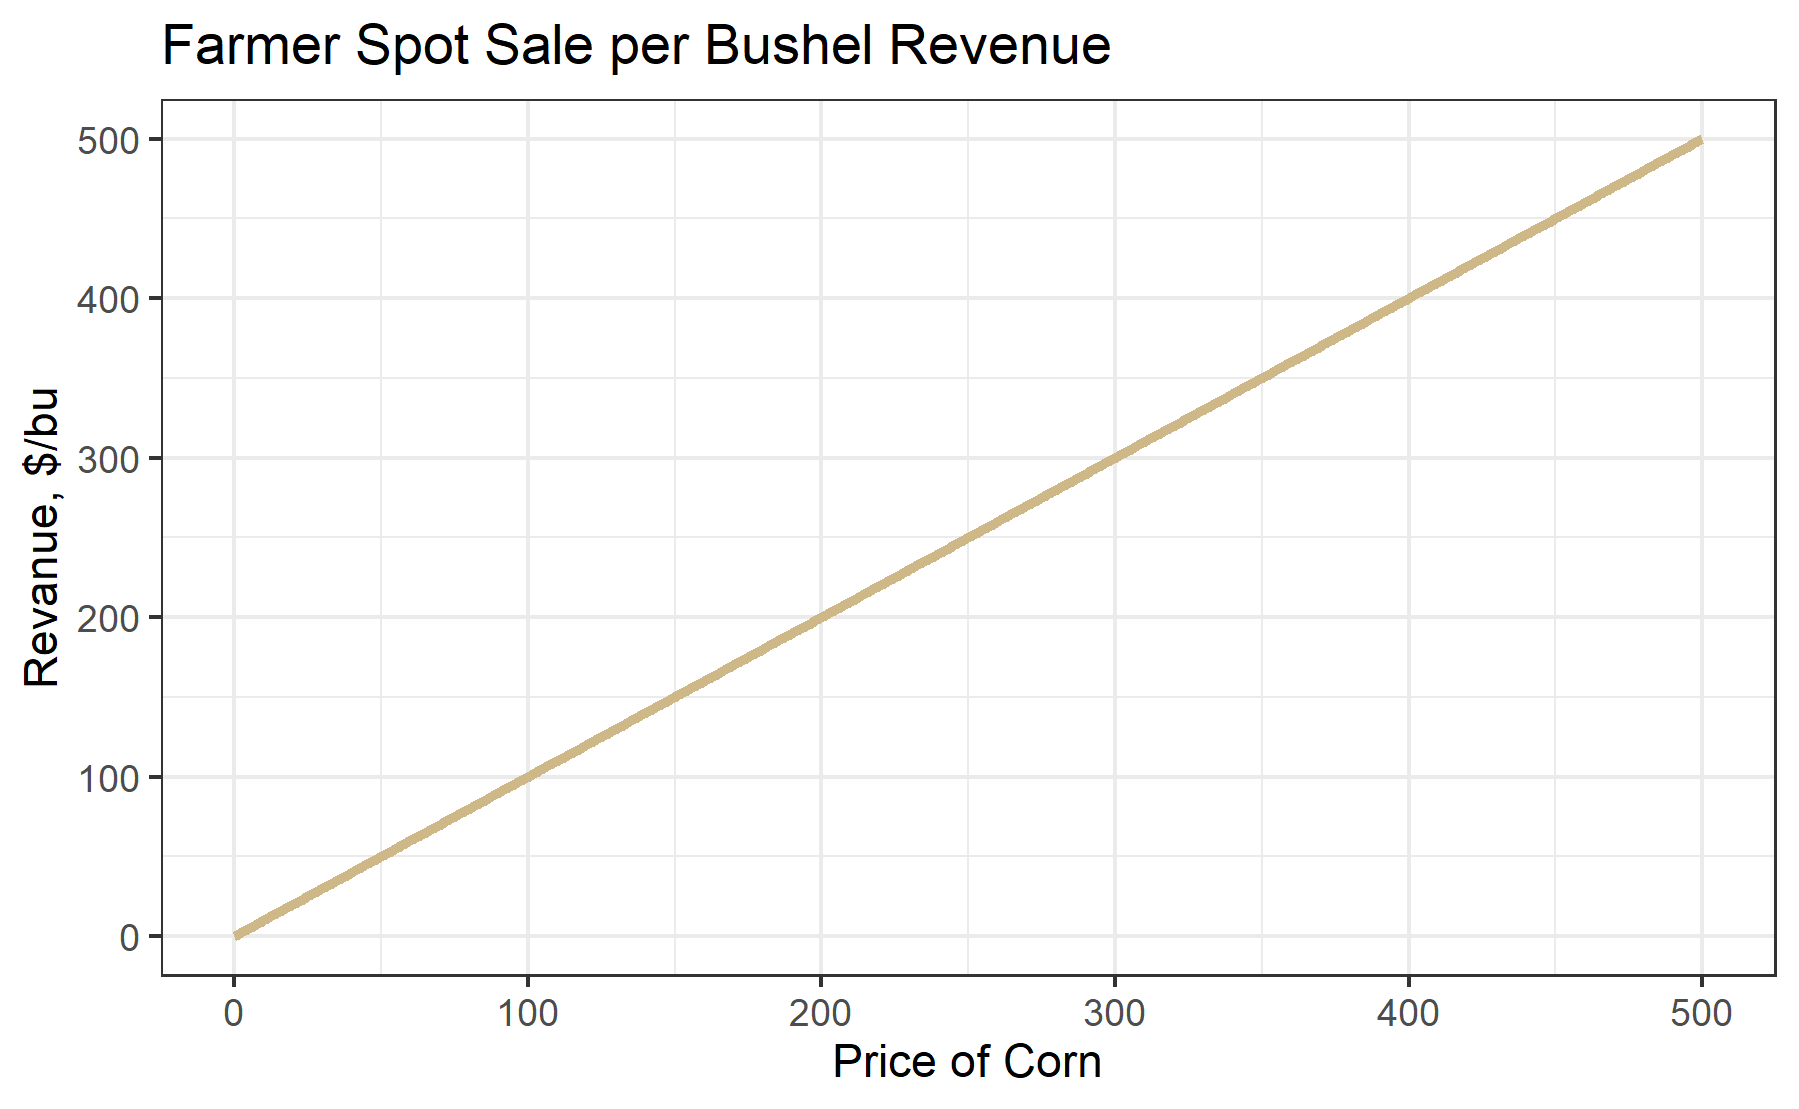
\includegraphics{assets/Options4-spot.png}

Next, add the payoff at expiration of a long 450 strike put option whose
premium is 17 cents per bushel.

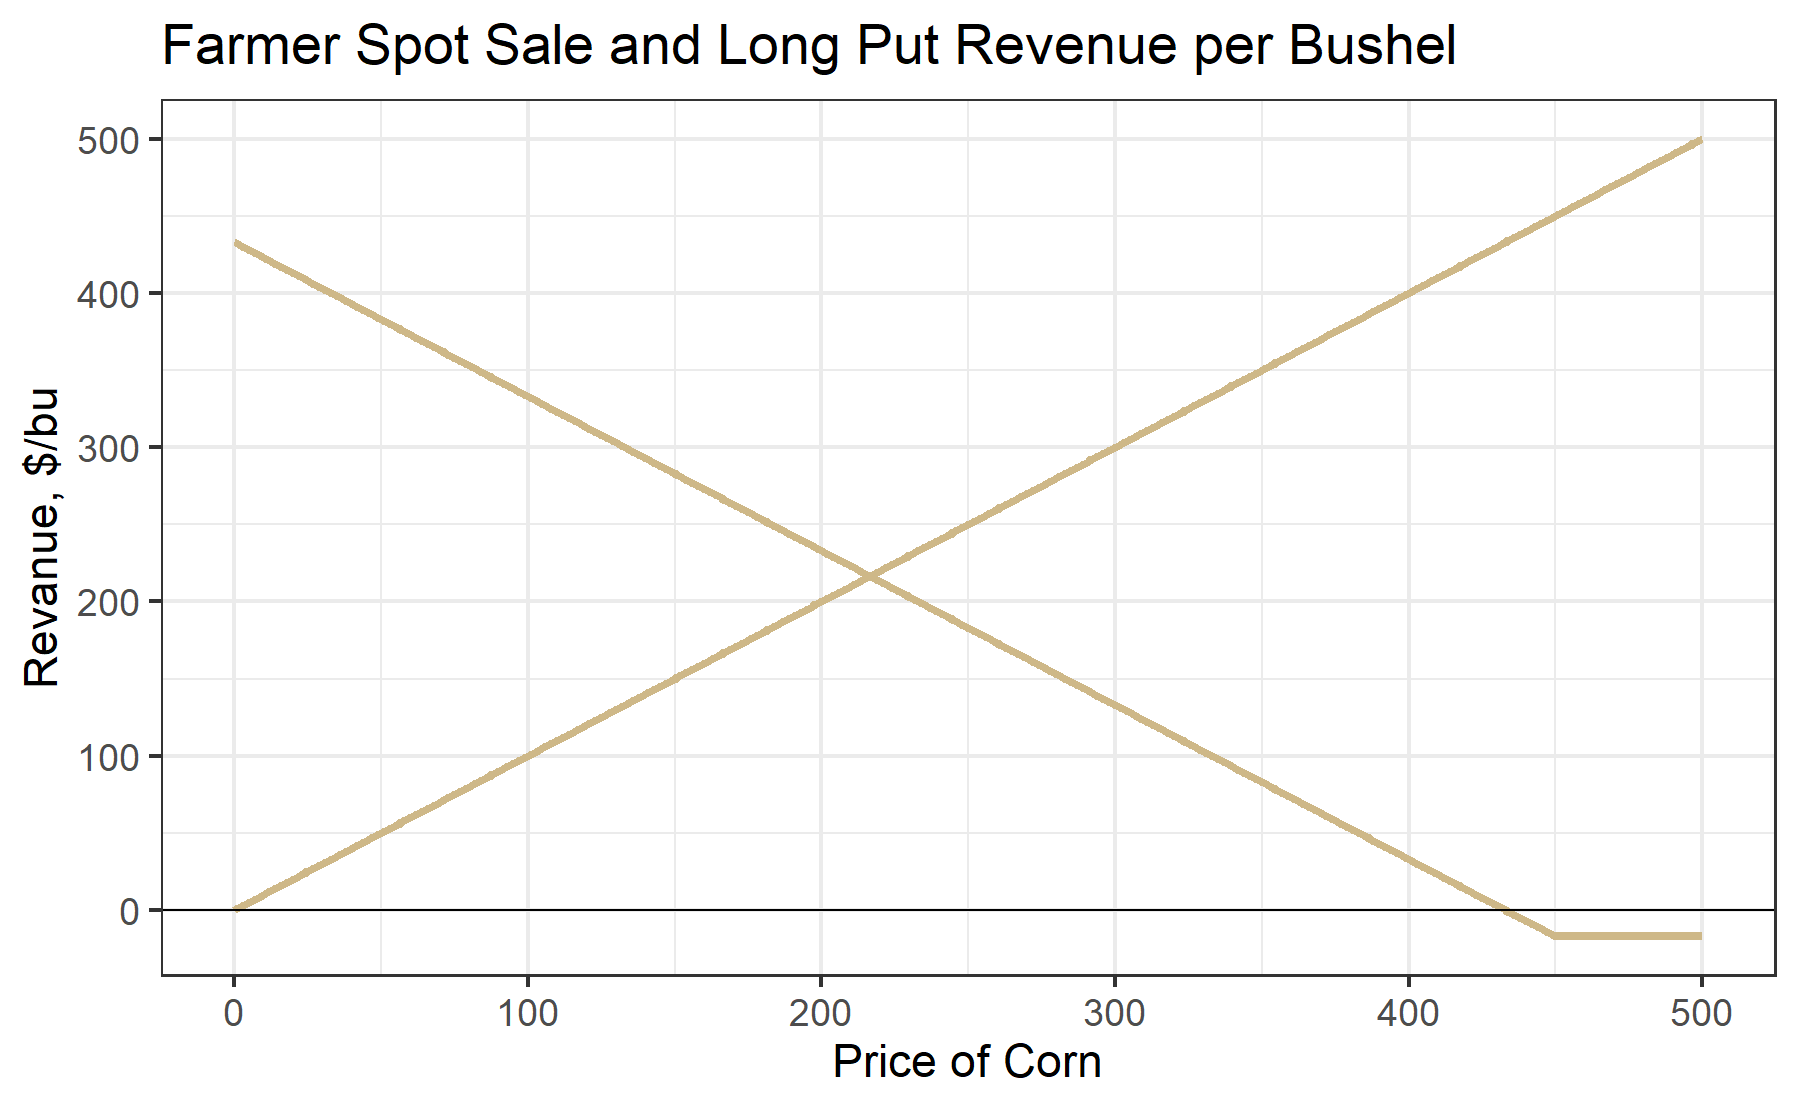
\includegraphics{assets/Options4-spotput.png}

If we add these two positions together, we get the net position shown by
the black line. The three most important things to note about this net
position are as follows: 1) Downside risk is capped at the strike of the
long put option, 2) Upside potential is preserved, but it is lowered by
the amount of the put option premium. That is, everywhere the black line
is upward sloped, it is lower than the spot revenue by the amount of the
put premium.

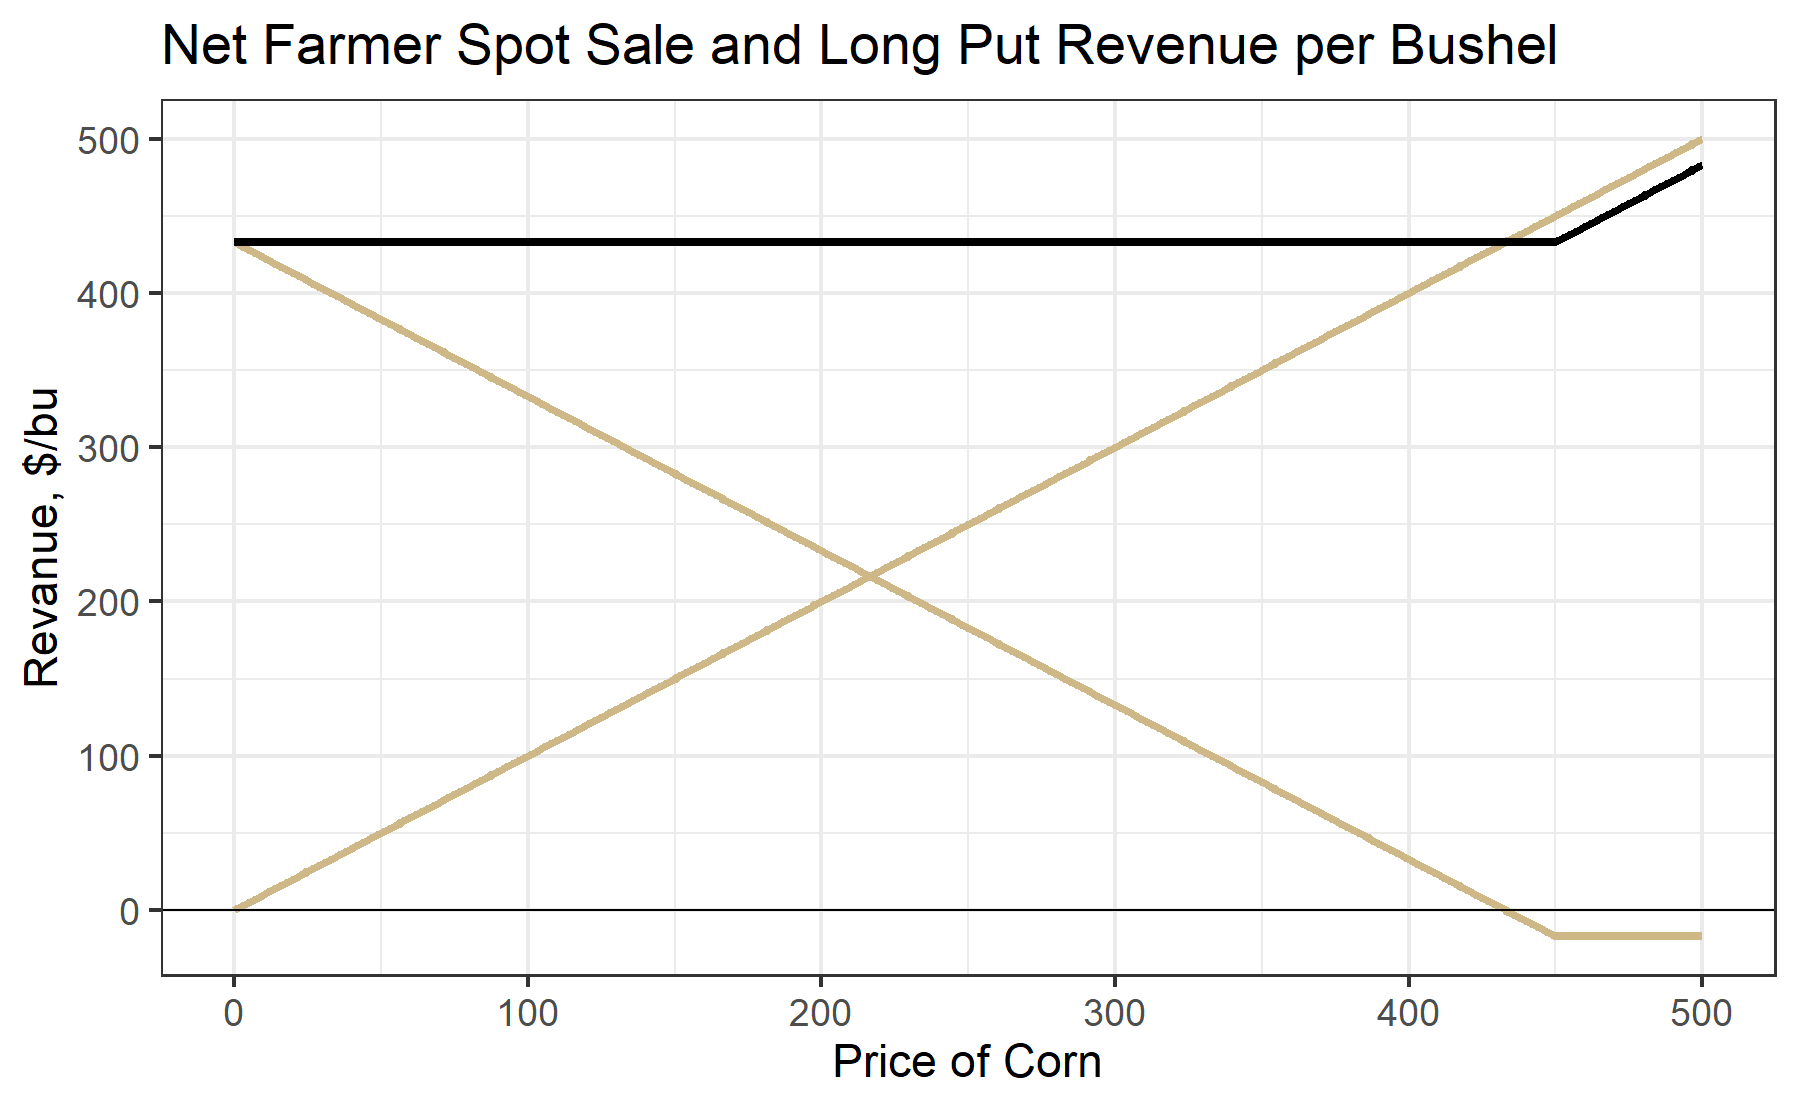
\includegraphics{assets/Options4-spotputcomb.png}

The figure below is the same as the previous figure, but zoomed in. Note
how the net position now looks a lot like holding a long call option
position. Long Spot + Short Put = Long Call.

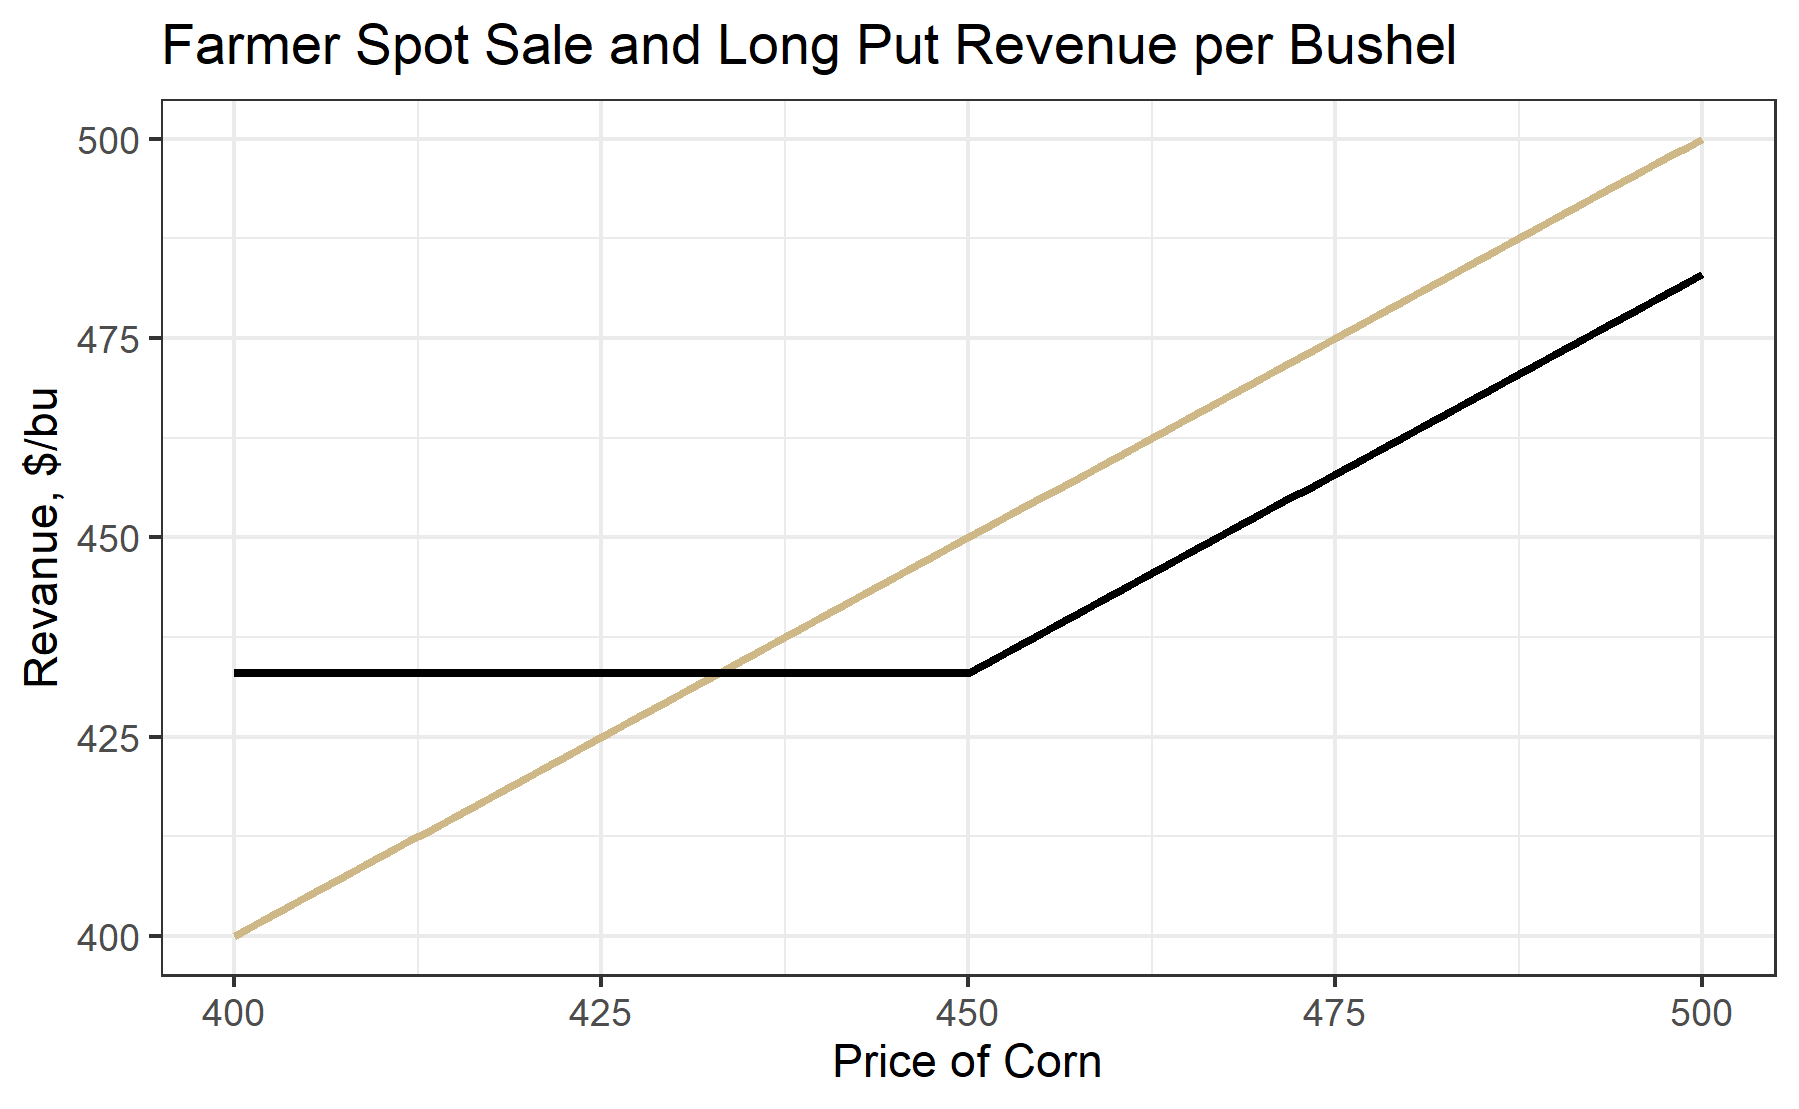
\includegraphics{assets/Options4-spotputcombzoom.png}

The strike of the long put should be chosen by considering the trade off
between greater downside protection and premium cost. The figure below
shows how choosing the 450 strike put (solid line and a higher premium)
versus the 425 strike put (dashed line and a lower premium) affects the
net position. As above, the gold lines are the individual instrument
payoff lines, and the black lines show the net from holding spot and
long put positions. Choosing the 425 strike put results in a lower cost
in premium paid, so the black dashed line is closer to the gold spot
line. However, there is more downside risk associated with the 425
strike put.

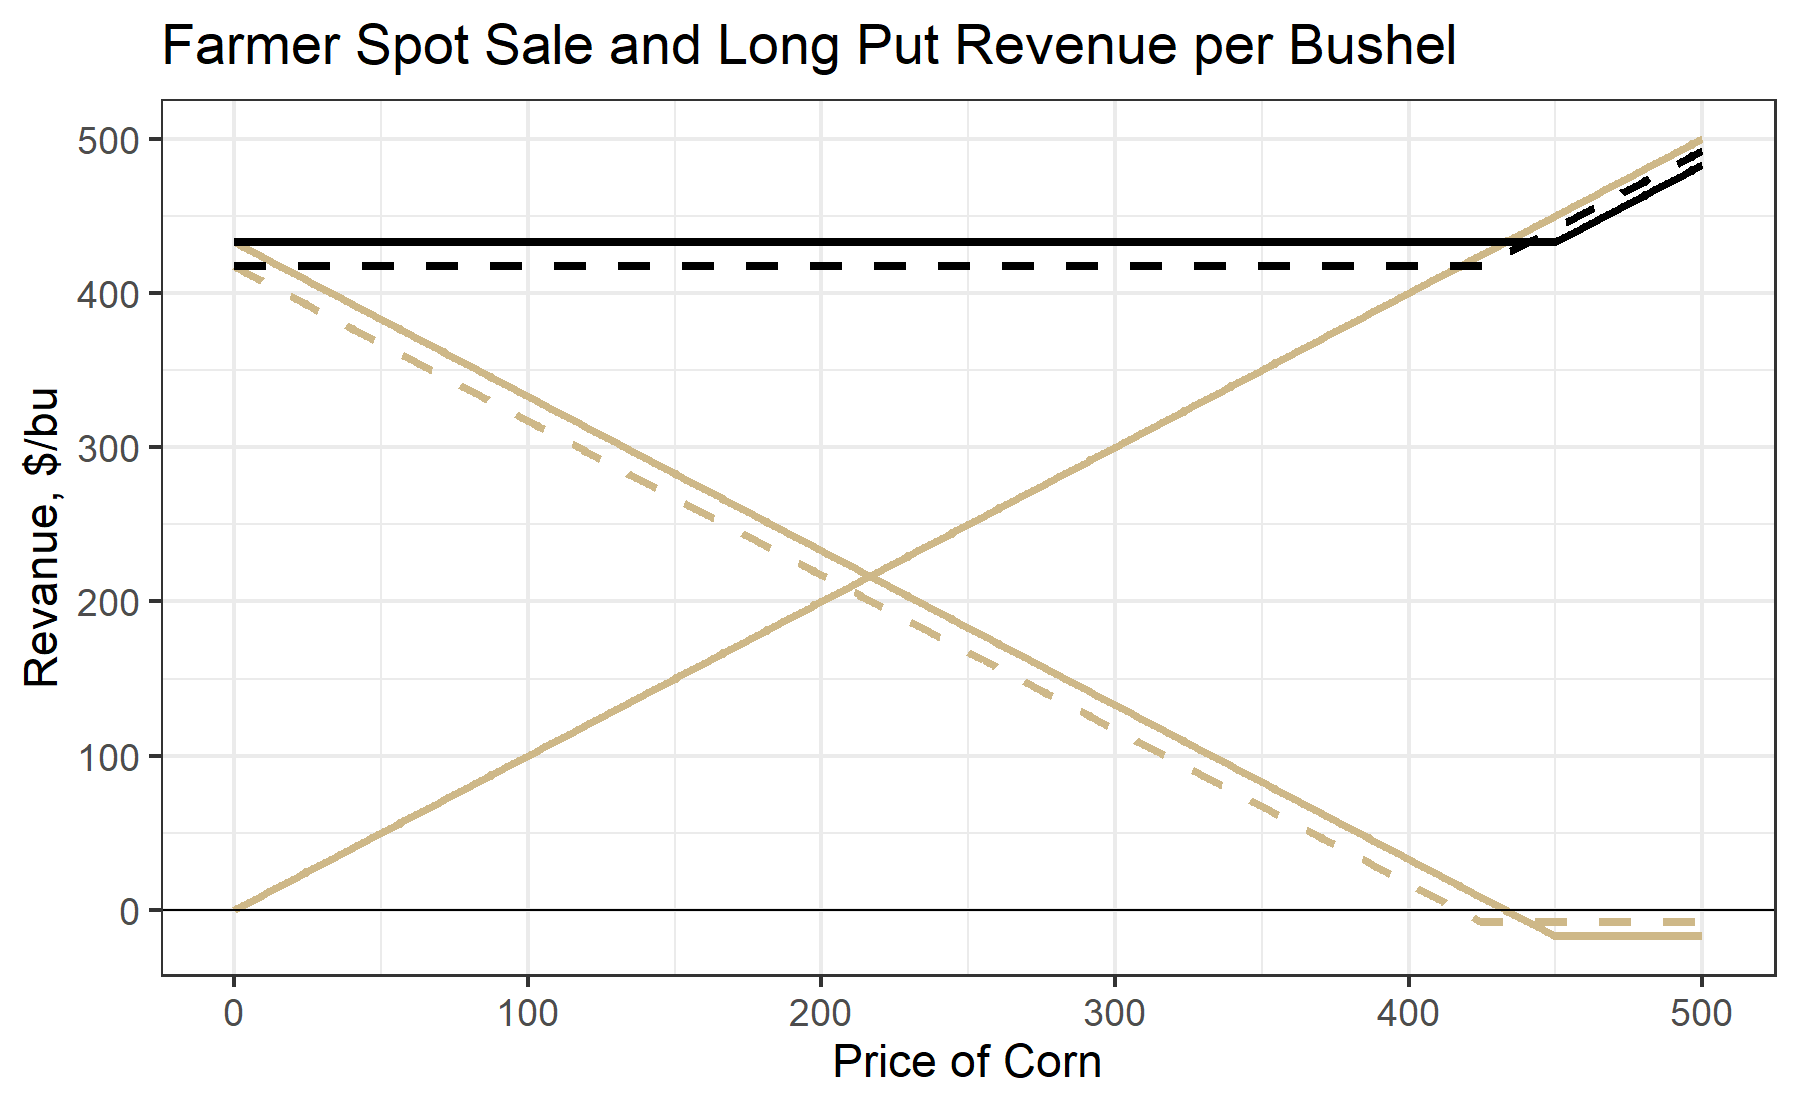
\includegraphics{assets/Options4-spotputcombzoomchoice.png}

A way to mitigate the cost of buying a put option to protect downside
risk is to sell a call option whose strike is above the current market
prices. Let's suppose current market price is 450, and we buy the 425
put for 7.85 cents premium and sell the 475 call for 13.5 cents premium.
You can see these individual positions in the figure below. If we sum
payoffs from all three of these separate positions you get the black
line. Below 425 there is no downside risk since you are protected by the
long put. Above 475 you do not enjoy additional gains because you sold
the call. In this case the upward sloped part of the black line is 13.5
- 7.85 = 5.9 cents above the gold spot line. However, whether you are
net positive or negative from the call premium collected minus the put
premium paid will depend on our strike choice. For example, if you
choose a tighter strike for the protective put, your downside is even
more limited, but the premium paid will be higher. Similarly, if you
choose a higher strike for the sold call you will retain more upside
potential, but the premium you receive will be smaller.

\section{Farmer Hedging by Putting on a
Fence}\label{farmer-hedging-by-putting-on-a-fence}

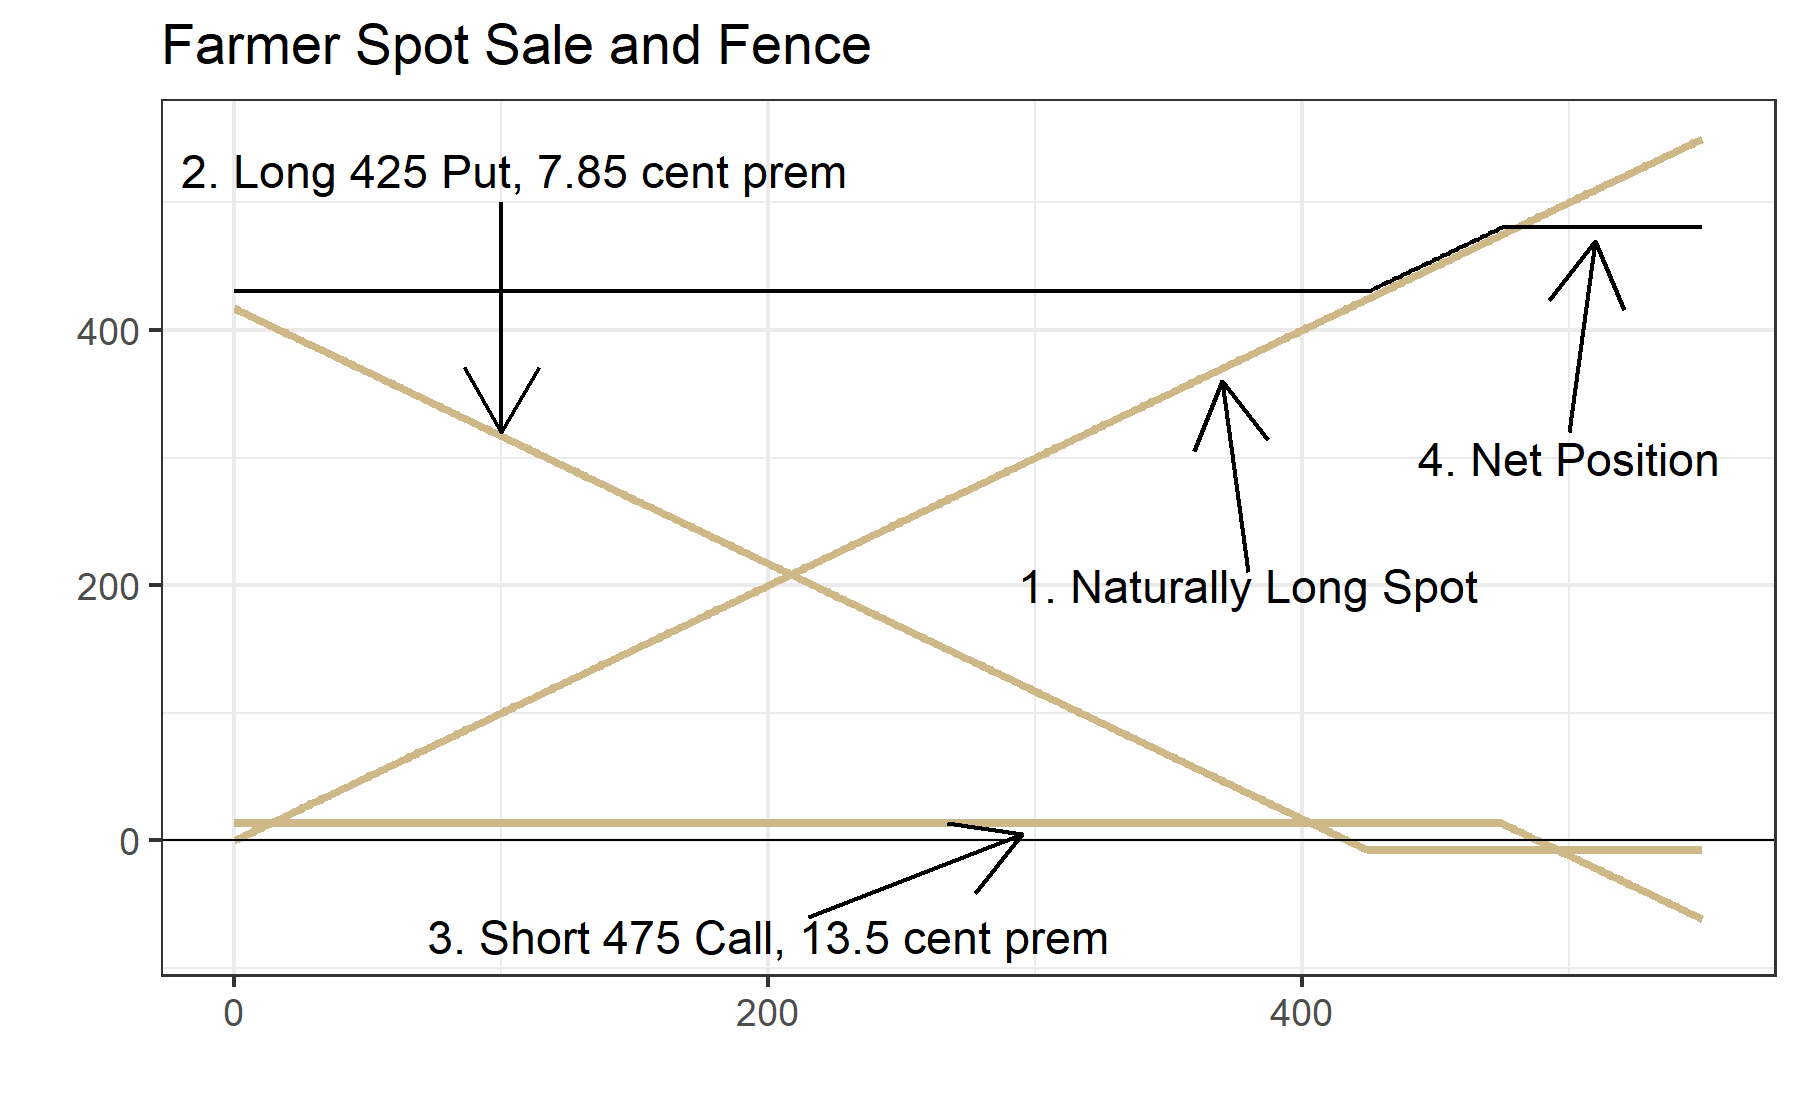
\includegraphics{assets/Options4-spotfence.png}

The essence of this strategy is that you are giving up some upside
potential to finance your expense in limiting downside risk. The figure
below gives a zoomed in view of the net position after putting on the
fence. The first kink in the black line is at the strike of the long
put, 425. The second kink in the black line is the strike of the short
call, 475.

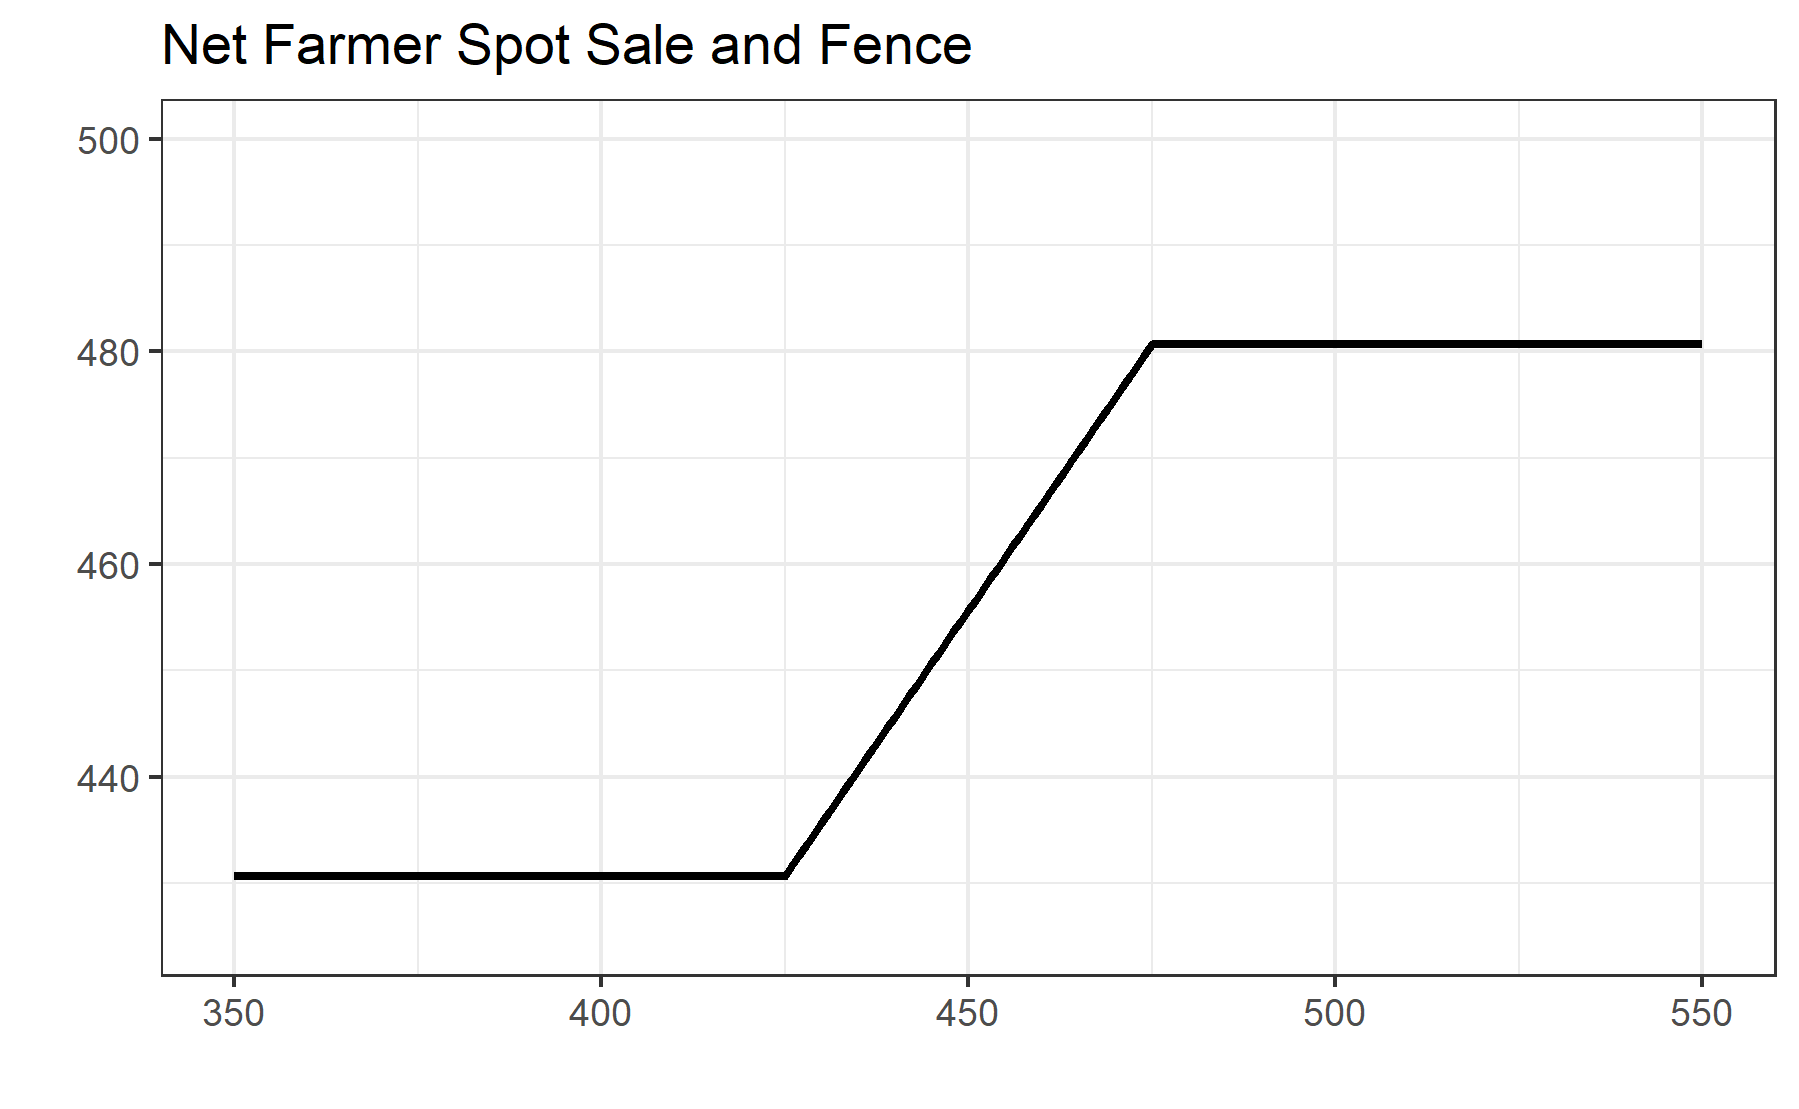
\includegraphics{assets/Options4-Netspotfence.png}

\subsection{A Note on Margin}\label{a-note-on-margin}

When putting on a fence, you have to keep in mind that your short call
position will require margin. If the price goes up, your short call
position will be losing money. Maintaining the position open will
require posting additional margin. To employ this strategy, you have to
be ready to lose the short call position, or have an agreement set up
with a lender to post margin in the event the price goes up enough to
wipe out your posted margin.

The long put position is fully paid up front, so that position does not
require margin posted to the account. As long as you have enough money
in your brokerage account to buy the option + fees, you can get into the
long put position.

\section{Wrapping Up}\label{wrapping-up}

In this chapter we learned how options can be used to hedge spot
positions in commodity markets. Downside risk can be protected with put
options, but this comes at significant cost in premium paid, especially
for options that have expirations longer than a week or two out.

\bookmarksetup{startatroot}

\chapter{Marketing, Hedging, and Crop
Insurance}\label{marketing-hedging-and-crop-insurance}

{Interested in more? Please let me know by}
\href{https://forms.gle/Q3VByCQZHjfQSy9D7}{taking the survey}!

\textbf{Highlights}

\begin{itemize}
\tightlist
\item
  Purchasing crop insurance provides protection against catastrophic
  loss in the event of crop failure, and/or significant price decline
  between planting and harvest
\item
  How much protection crop insurance alone provides varies based on
  pre-harvest price movements
\item
  Crop insurance alone does not provide an optimal marketing plan for
  some scenarios of price movement planting-harvest
\end{itemize}

\textbf{Check Your Understanding}

\begin{itemize}
\tightlist
\item
\end{itemize}

\section{Brief History of Crop Insurance Prior Federal Farm Support
Programs}\label{brief-history-of-crop-insurance-prior-federal-farm-support-programs}

Currently crop insurance dominates the landscape of federally sponsored
farm programs for risk management (Walters and Preston 2017). However,
the history of market interventions and price supports in the United
States is long and varied. Understanding the economic and political
motivations for moving from price supports and ad hoc disaster payments
(payments made when there is a large unexpected crop failure) to
federally subsidized crop insurance is interesting, However, a full
account is beyond the scope of this chapter. Readers can refer to the
following for additional historical context (Babcock and Hart 2006; J.
Glauber and Effland 2016; Cochran 1951; Marcus and Modest 1986;
Lichtenberg and Zilberman 1986; {``History of Agricultural Price Support
and Adjustment Programs''} 1984).

The short story is that price supports can distort markets by creating
inefficiency in production decisions and generate ill will with trading
partners through subsidizing too much production and lowering world
prices to the detriment of farmers in other countries. Further, ad hoc
disaster payments are by nature not predictable in the timing of when
they are needed nor in the size of the need. Both of these created an
appetite among lawmakers for a farm support program whose cost was more
predictable.

Over the last 30 years crop insurance has come to be the dominant way in
which federally sponsored risk management is administered to commodity
producers. Two challenges had to be overcome, however.

First, crop insurance is a product that is not possible to be offered
exclusively by the private sector. Insurance markets can exist in the
private sector when the insured losses are relatively small (compared to
premium collected) and predictable from year-to-year (Babcock and Hart
2006). Crop insurance is neither of these things because 1) losses are
typically highly correlated. When there is a crop failure, most farmers
in the affected region experience a loss and make a claim on the policy.
This makes it very hard for a private insurance company to ensure they
have enough liquidity to pay for losses in the event of a widespread
crop failure. Therefore, without a federal backstop to the policies, the
private market could never offer crop insurance.

The first crop insurance programs administered by the federal government
from the 1930's to the 1980's did not attract sufficient usage among
farmer to prevent the passage of additional ad hoc disaster payments (J.
W. Glauber 2013). This is a problem because the administration of the
federal crop insurance program is costly, so if taxpayers have to pay to
administer the crop insurance program \emph{and} pay for ad hoc disaster
from time-to-time, the program is not meeting its purpose and wasting
taxpayer money at the same time by paying for two solutions (Babcock and
Hart 2006).

A series of reforms through the 1980's and 1990s including the Federal
Crop Insurance Act of 1980 and the Crop Insurance Reform Act of 1994 led
first to making purchase of crop insurance coverage mandatory for
farmers to receive other program payments. Then the mandatory coverage
requirement was removed in favor of premium subsidies. Congress
increased the subsidy rate for crop insurance premiums to levels where
farmers voluntarily purchase enough coverage to reduce the need for
frequent disaster payments. At the time of writing, federal subsidies
for crop insurance average 62\% of the premium cost (Zulauf 2016).

\section{Overview of Typical Crop Insurance
offerings}\label{overview-of-typical-crop-insurance-offerings}

\textbf{Yield Protection and Area Yield Protection}

Yield Protection guarantees against a loss of production less than a
percent of Actual Production History (APH). Indemnities are paid when
production falls below the APH and are paid based on that production
year's projected price (for corn and soybeans this is an average of the
new crop futures settlement prices during February). Area Yield
Protection is similar, but the yield guarantee is based on county
yields, not the individual producer's.

\textbf{Revenue Protection and Area Revenue Protection}

Revenue protection guarantees against loss of revenue below the APH
times the greater of the projected price (new crop price in February)
and the harvest price (the new crop price at harvest). Since farmers are
concerned with revenue loss, not necessarily yield loss, this type of
contract gained popularity.

Area Revenue Protection, similar to Yield Protection, calculates the
revenue guarantee against the county APH rather than the producer's APH.

\textbf{Revenue Protection with Harvest Price Exclusion}

Revenue protection with Harvest Price Exclusion is the same as Revenue
Protection, except the policy doesn't guarantee based on the Harvest
Price, Revenue is calculated based on the Projected price times APH.

\section{Pre-Harvest Marketing Strategies Paired with Crop Insurance
Protection}\label{pre-harvest-marketing-strategies-paired-with-crop-insurance-protection}

Now we turn our attention to marketing strategies that can complement
crop insurance, since roughly 90\% of U.S. cropland is insured in some
way in the Federal Crop Insurance program(Farrin, Miranda, and
O'Donoghue 2016). The rest of this section will consider marketing
strategies to lock in a forward price of \emph{insured} bushels. Note
that marketing uninsured bushels is very risky in the event of a crop
failure. For example, suppose you entered into a forward contract to
deliver 1000 bushels of corn at \$5.00 per bushel, but you experienced
yield losses so that you only made 500 bushels. You cannot meet your
obligation to deliver 1000 bushels. In this case you will have to buy
out the contract. You will have to buy 500 bushels in the spot market.
Unfortunately for you, your crop failure is likely to be correlated with
low production for many farmers, so prices are likely to be high.
However, if you have Revenue Protection crop insurance, you are
guaranteed coverage percent X APH X max(Base Price, Harvest Price). This
revenue guarantee ensures you can at least buy out your forward contract
in the event of a crop failure.

Second, from a hedging perspective the marketing decision is trivial if
prices fall after the base price is set. You are already have revenue
protected at a level of coverage level X APH X Base Price. So if price
falls you are already hedged. If you take a bullish or bearish position
you are a speculator at that point.

It does become an interesting marketing question in the case where the
price rises after the Base Price is set at the first of March. The
producer is exposed to price uncertainty to both the upside and
downside. However, with revenue protection, revenue is guaranteed at the
harvest price unless price falls below the Base price.

Such a scenario is shown in the figure below. Also in this assumption is
that the Base Price of \$5.00 is above the BreakEven Price of \$4.90.
Then, suppose as of July the December corn futures price is \$5.35, a
substantial rise above the Base Price. Should a producer lock in this
high price?

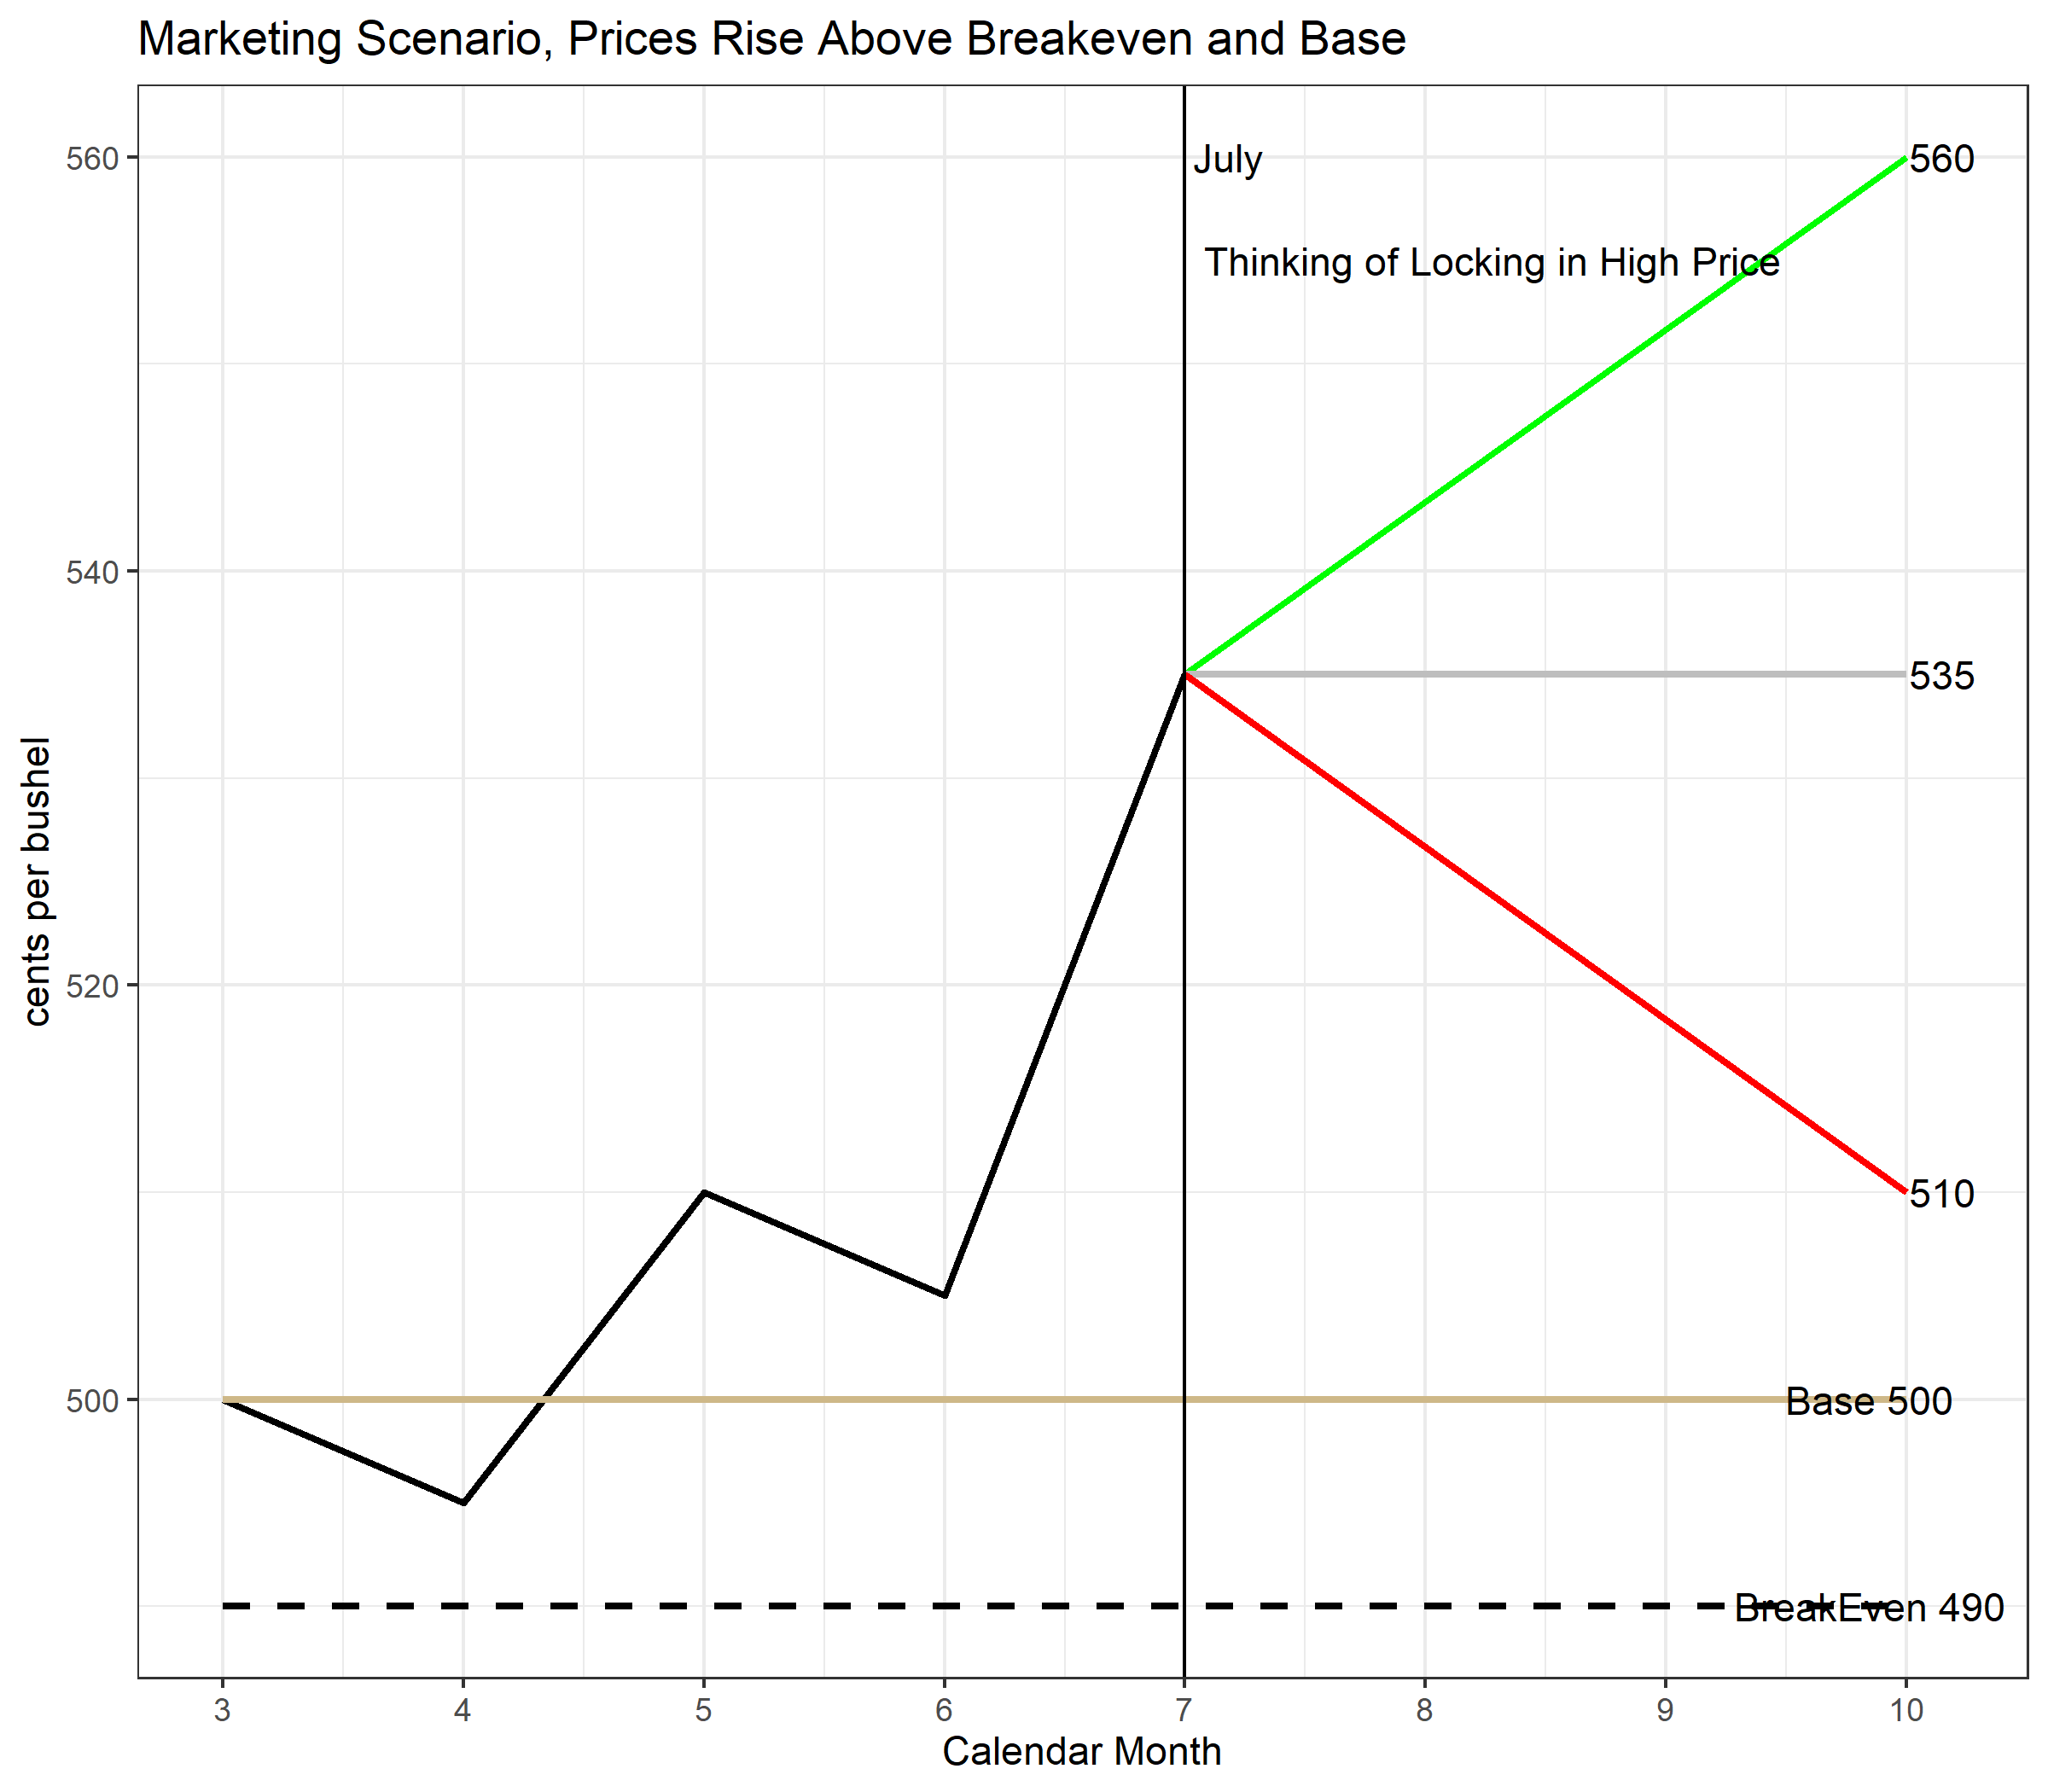
\includegraphics{assets/cropins_ex.png}

To simplify our thought experiment, suppose that from July to October
the price might do one of three things, rise to \$5.60, stay flat at
\$5.35, or fall to \$5.10. We will examine the following marketing
choices: selling futures, or contracting for harvest delivery (we will
assume zero basis to keep that part simple). Also, we will examine what
happens if you make 100\% of your APH, and what happens if you make 80\%
of your APH. For the sake of example, assume the APH is 200 bushels per
acre, and coverage level on Revenue Protection policy is 85\%. You can
explore the moving parts yourself by going to the Google sheet
\href{https://docs.google.com/spreadsheets/d/1rbne8odUljxIuIYP3IRiWyzaQDs83-mjOkuaaDWxb3w/edit?usp=sharing}{here}.

\bookmarksetup{startatroot}

\chapter{Prices Over Space and Time}\label{prices-over-space-and-time}

{Interested in more? Please let me know by}
\href{https://forms.gle/Q3VByCQZHjfQSy9D7}{taking the survey}!

\textbf{Highlights}

\begin{itemize}
\tightlist
\item
  Learn the costs of storage for farmers.
\item
  Learn how the forward curve in the futures market provides incentive
  to store that can be `locked in'.
\item
  Learn how to calculate financial full carry and spread as a percent of
  full carry.
\item
  Learn how to interpret the percent of full carry as a measure of
  incentive to store.
\item
  Learn what drives variation in the basis.
\end{itemize}

\textbf{Check Your Understanding}

\begin{itemize}
\tightlist
\item
  Can you calculate the percent of full carry yourself, given only
  futures prices and financing costs?
\end{itemize}

In this section we cover how commodity prices behave over time and
space. We have discussed frequently that commodity futures contracts
have an expiration, that there are always several contracts trading at
any given time with maturities that are increasingly farther into the
future, and that these contracts will eventually expire and no longer be
traded.

The contract that is next to expire is called the \textbf{Nearby}
contract, the contract that expires next is called the \textbf{First
Deferred} contract, the contract that expires after that is the
\textbf{Second Deferred} contract. The different contracts trading at
any given time make up make up what is called \textbf{The Forward
Curve}, etc. There is valuable information in the forward curve because
it is the market's best guess of what returns to storage will be.

We saw in Chapter 4 how a farmer can use the December futures contract
to hedge the sale of their harvest. Similarly, the March (of the next
year) contract is the next to expire after the December contract. If the
market price of the March contract is high enough, some farmers (and
other commercial stockholders\footnote{Stockholder here means an entity
  who is storing grain (or oilseed). In other-words, they are holding
  stocks of the grain.}) will decide to store until late February and
hedge their cash sale with the March futures contract. This is costly so
the price increase from waiting until March must be high enough to cover
these costs or the farmer will just sell everything at harvest.

\section{Storage Costs to the Farmer}\label{storage-costs-to-the-farmer}

Storage costs include the following:\footnote{For more
  \href{https://www.extension.iastate.edu/agdm/crops/pdf/a2-33.pdf}{see}}

\begin{enumerate}
\def\labelenumi{\arabic{enumi}.}
\tightlist
\item
  Opportunity cost of money. If they sell at harvest they can use the
  money for other things; so waiting to sell involves an opportunity
  cost of money.
\item
  Interest. By deferring the sale of grain, the stockholder may need a
  bank loan to cover expenses since their main revenue stream is
  deferred.
\item
  Storage fees. Some farmers or stockholders have their own storage
  space, but many will need to rent storage space (from an elevator like
  the one depicted in Royal, IL in chapter 4).
\item
  Drying costs. Grain that is just harvested can be around 15\%
  moisture, but must be dried down to closer to 13.5\% moisture to
  safely store for long periods. This involves running a grain dryer
  that uses fuel and/or electricity.
\item
  Shrinkage. When grain is dried, it actually shrinks leaving less
  bushels to sell after storage. The shrink factor can be 1.25 to 1.4
  percent.
\item
  Quality deterioration. If the grain is not stored under proper
  condition, quality can deteriorate, and result in dockage (a price
  discount) being applied by the buyer at the time of sale.
\item
  Cost of handling. Getting the grain into and out of storage results in
  some costs as well.
\end{enumerate}

Iowa State University Extension estimated in 2015 that storing grain
until March costs a farmer roughly \$0.45 per bushel, while storing
until December cost roughly \$0.30 per bushel, \$.15 cents per bushel
less than storing until March. Considering only this, the price of the
March contract would need to be more than \$0.15 per bushel higher than
the December contract to cause much grain to be stored until
March.\footnote{Ed Usset with the University of Minnesota Extension has
  a nice series of articles in Corn and Soybean Digest about
  \emph{carrying charges},
  \href{http://www.cornandsoybeandigest.com/marketing/understand-carrying-charges}{here},
  \href{http://www.cornandsoybeandigest.com/carrying-charges-part-1}{here},
  and
  \href{http://www.cornandsoybeandigest.com/carrying-charges-part-2}{here}.}

\section{An Increasing Forward Curve}\label{an-increasing-forward-curve}

Figure 1

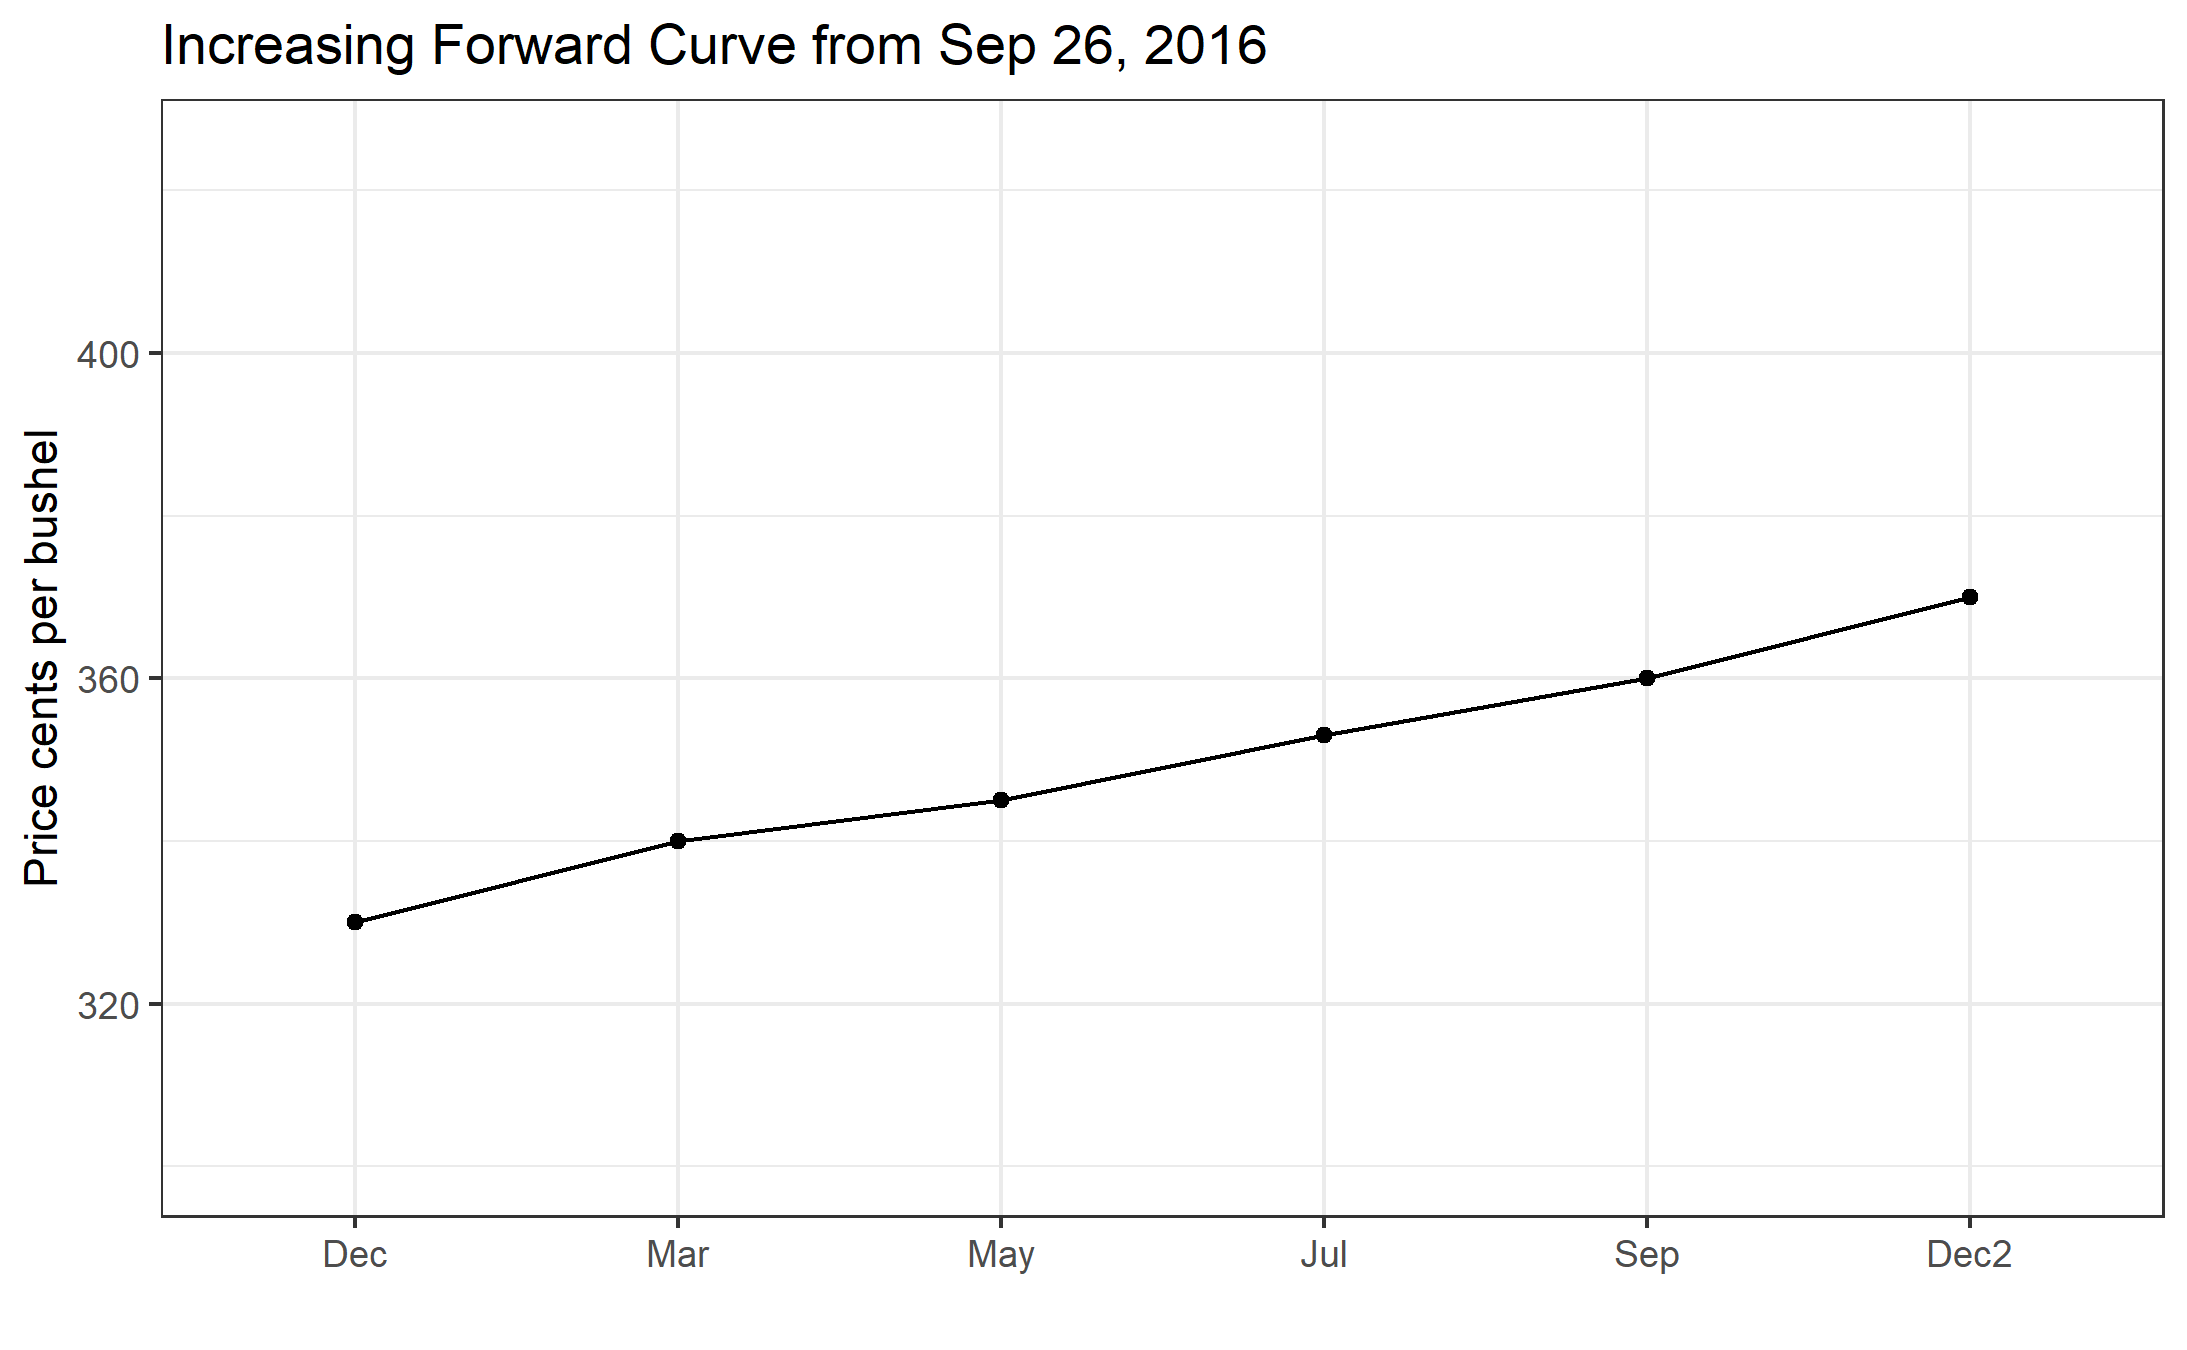
\includegraphics{assets/PricesSpaceTime-increasing-9-26-2016.png}

The reason that the forward curve represents return to storage is that
it shows how much extra money can be made by storing to a later date,
rather than selling in the cash `spot' market today. December corn is
worth 330 cents per bushel and March corn is worth 340 cents per bushel,
then you can make an extra 10 cents per bushel by selling the March
futures and selling into the cash market later.

When stocks are plentiful the market offers a premium to those who are
willing to keep grain off the market for awhile. This prevents prices
from plunging too much right after a big harvest, since many choose to
wait for better prices later in the marketing year. Also, since these
price relationships are `discovered' and change every day, if it turns
out grain is coming onto the market too fast or too slowly, the shape of
the forward curve changes to alter the incentives so that supply and
demand can remain in equilibrium throughout the whole marketing year
even though we only harvest once per year (in North America).

This kind of market environment is sometimes called a \emph{carry
market} or \emph{contango market}, or sometimes it is said that the
market is \emph{in full carry}. This means that the market is offering
returns to storage that covers the cost to rent warehouse space, insure,
and finance storing grain in until a later date. The year of 2016 was
certainly a full carry market. Record production and a high forecast of
ending stocks make this the classic market environment where returns to
storage would be positive.

As another example, the forward curve is shown for 2015 in figure 2.

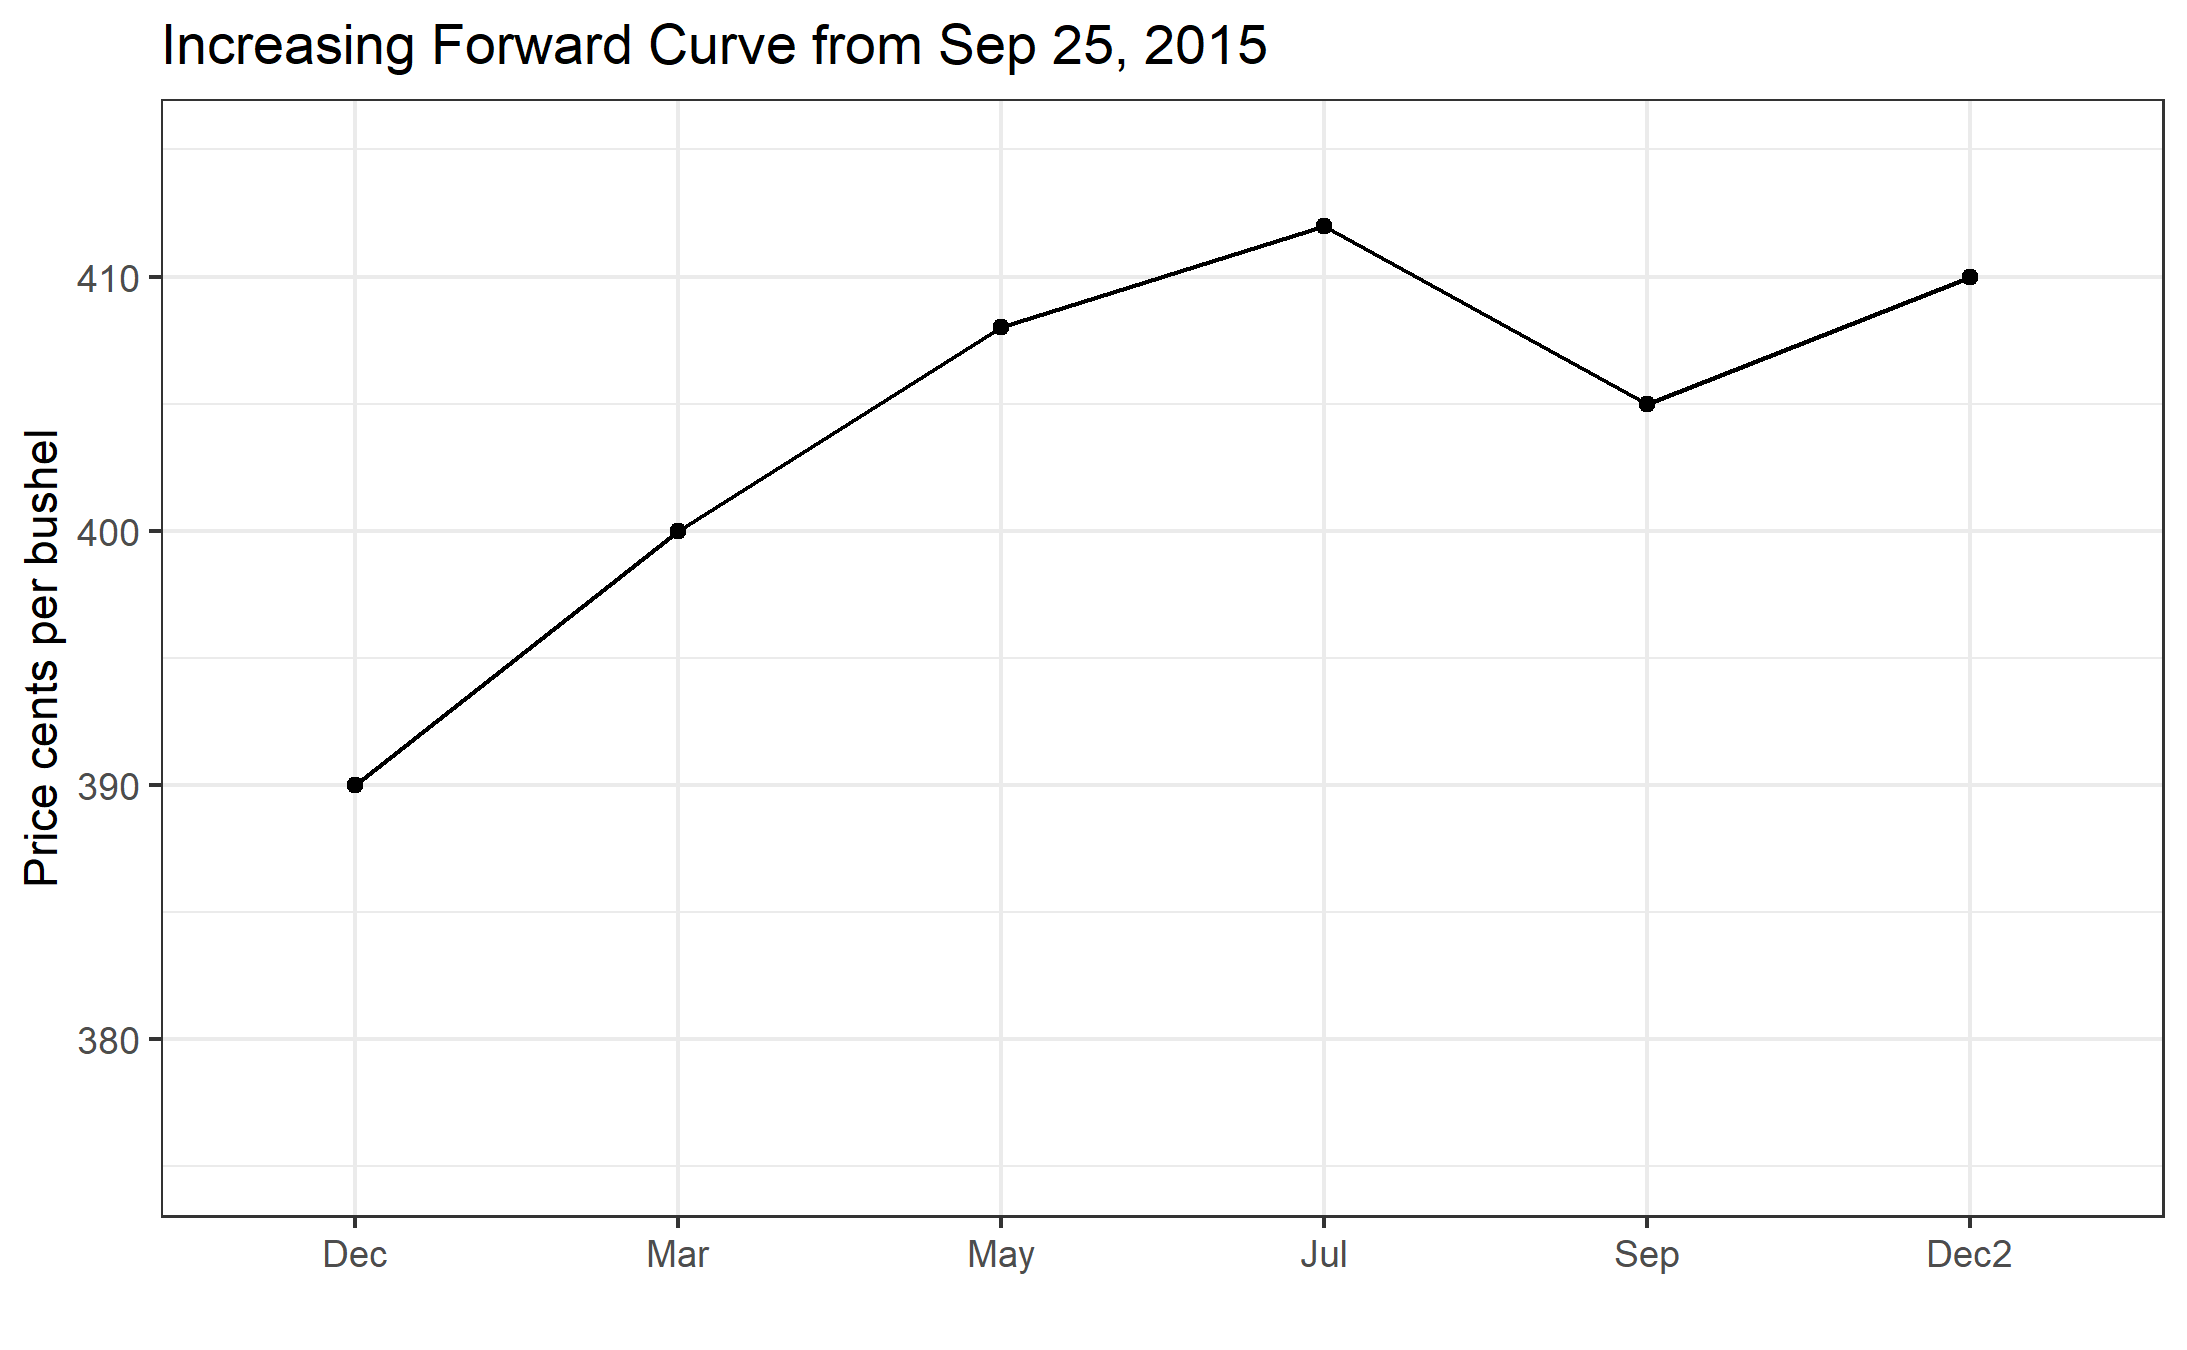
\includegraphics{assets/PricesSpaceTime-increasing-9-25-2015.png}

This example illustrates a phenomenon that often occurs. Here we saw
that the forward curve is upward sloped until September. Then it
flattens and returns to storage go away. This makes sense because in
September we begin to see some of the next year's crop come onto the
market. So in 2015, the market was basically asking farmers to keep
storing through July, but no longer. Anyone planning to hold grain from
July to September and beyond could expect to lose as much as 4 cents per
month.

\section{A Decreasing Forward Curve}\label{a-decreasing-forward-curve}

Next we will consider a year that was characterized by a decreasing
forward curve. You will recall that 2012 was a significant drought year
that resulted in poor yields, high prices, and low forecasted ending
stocks for the marketing year. In this kind of market environment, where
supplies are tight, the forward curve tends to be downward sloped. The
implication of this is that anyone who decides to hold grain will lose
money because it is worth more today than it is tomorrow. The market is
incentivising everyone to bring grain onto the market.

We will look at the forward curve and return to storage in steps for
2012. On 4-13-2-12 the forward curve are as shown in figure 3. This is
in the spring, before the drought has happened.

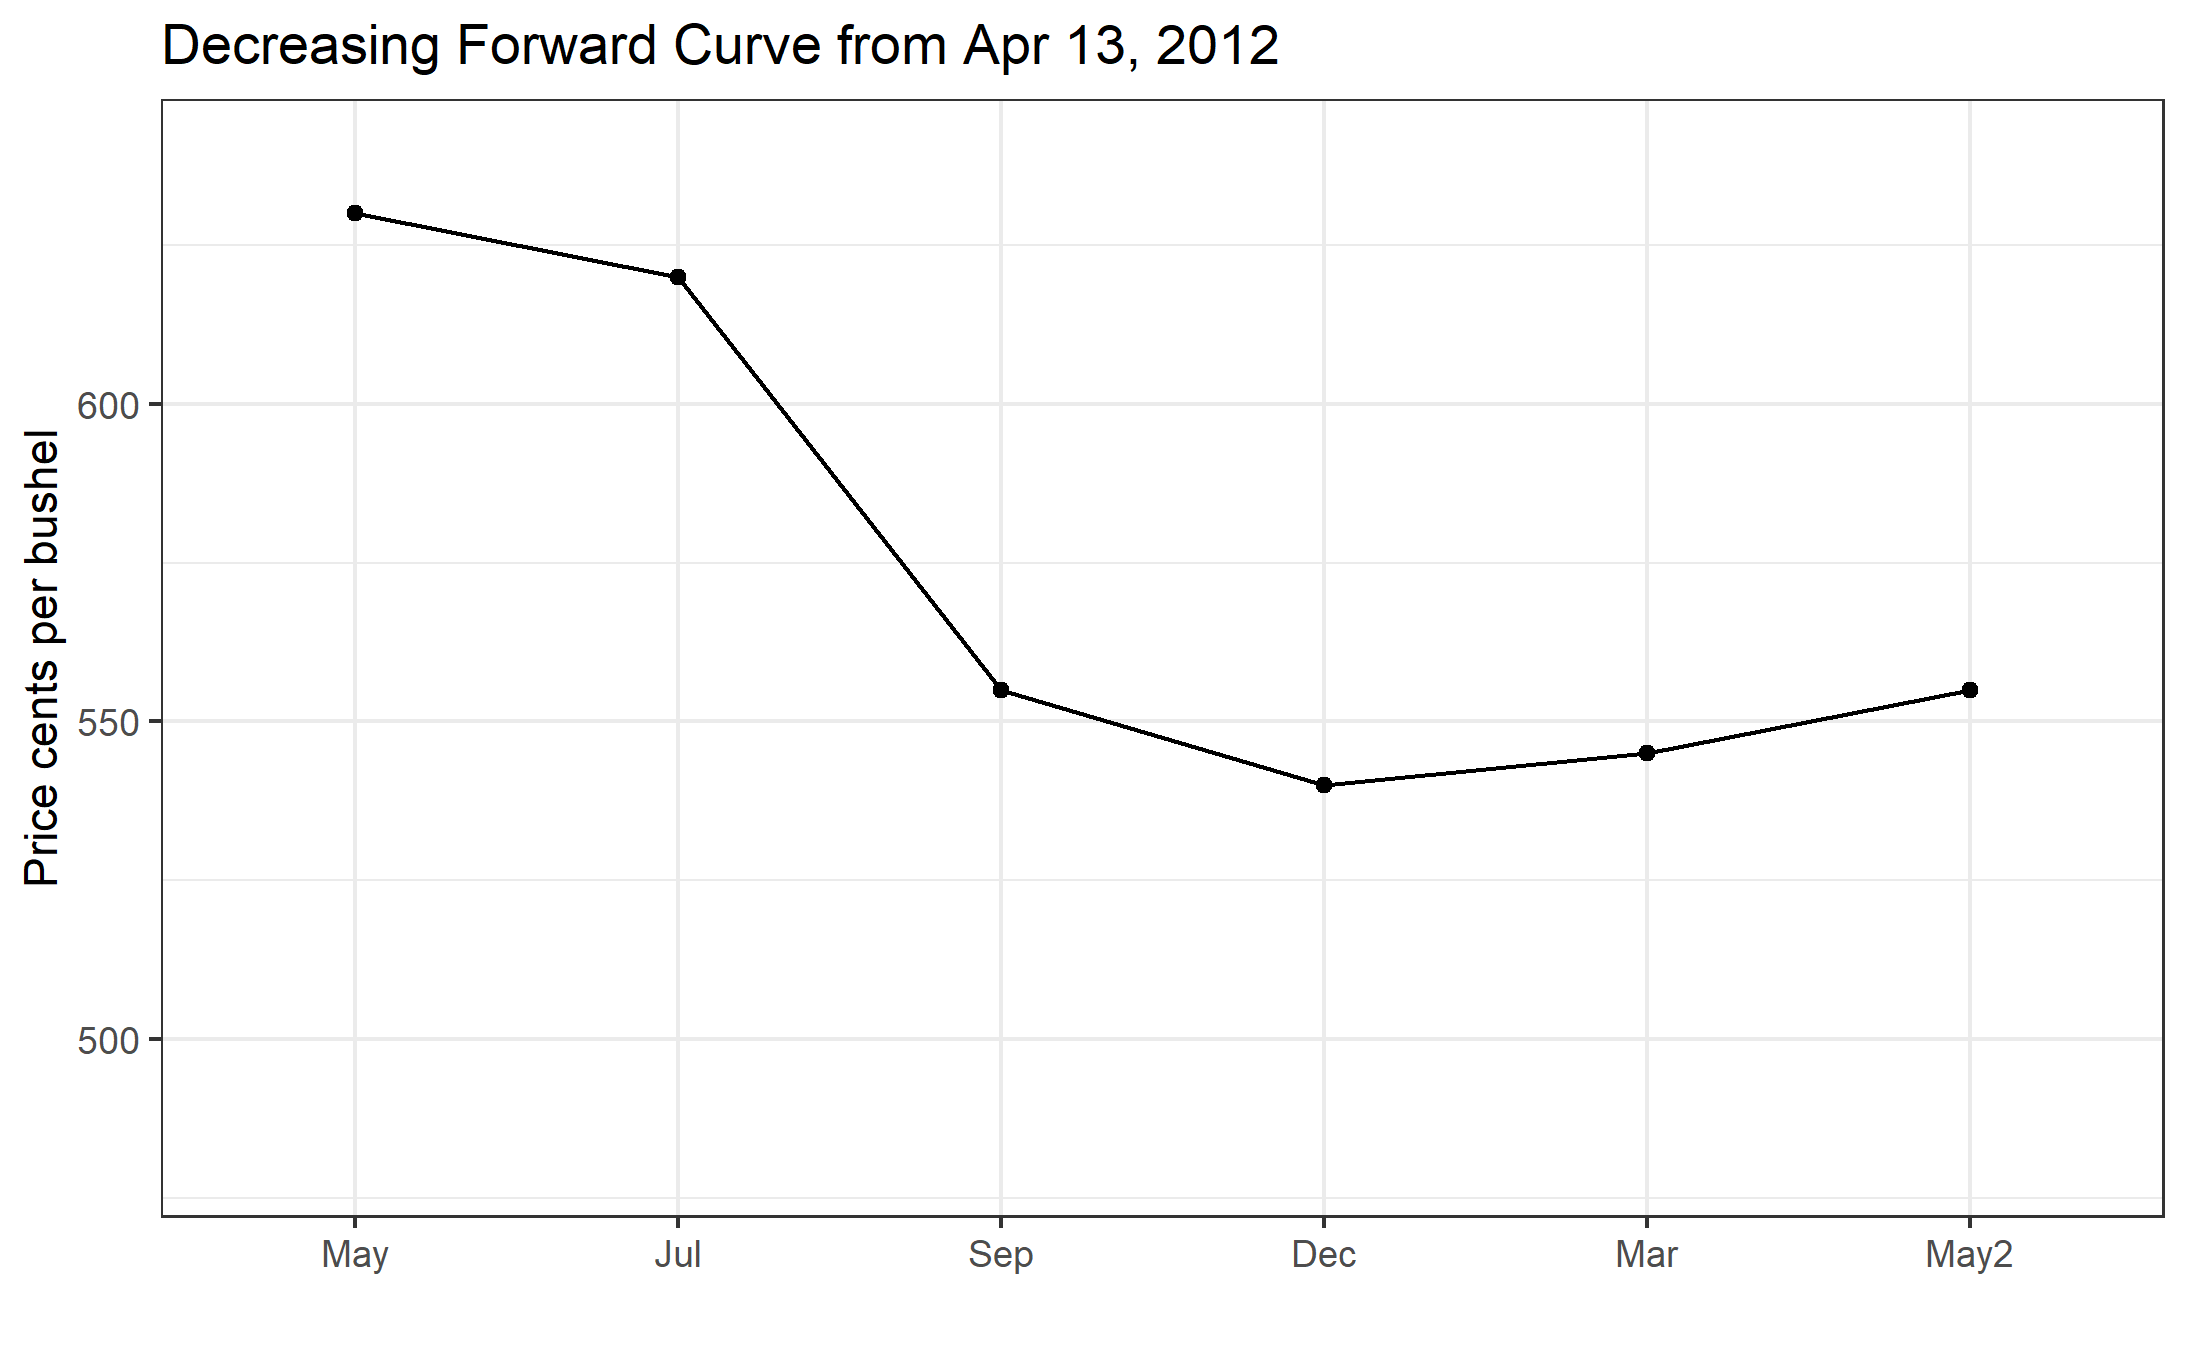
\includegraphics{assets/PricesSpaceTime-decreasing-4-13-2012.png}

In this case, supplies were already tight going into 2012. The forward
curve is downward sloped, sometimes called \emph{inverted} or
\emph{backwardated} market. So returns to storage are negative, as shown
in Figure 6 through the summer of 2012, even before we had the drought
realized. However, it is apparent from the forward curve that as of
4-13-2012, the market `thought' that the 2012 harvest would be good,
because price levels drop substantially in the September and December
contract, and the return to storage between December 2012 and March 2013
is positive on 4-13-2012.

Next, lets look at the forward curve on 8-01-2012. By August 1, it is
clear that we are in the midst of a major drought, yields will be low,
and ending stocks for the coming marketing year will be low as well.

Now, the forward curve is downward sloped for the entire marketing year
until the next harvest, in 2013, is expected. On 4-13-2012, the market
was offering about 5 cents per month to store from December 2012 to
March 2013, by 8-01-2012, the market was offering -1 cent for storage
during the same time period.

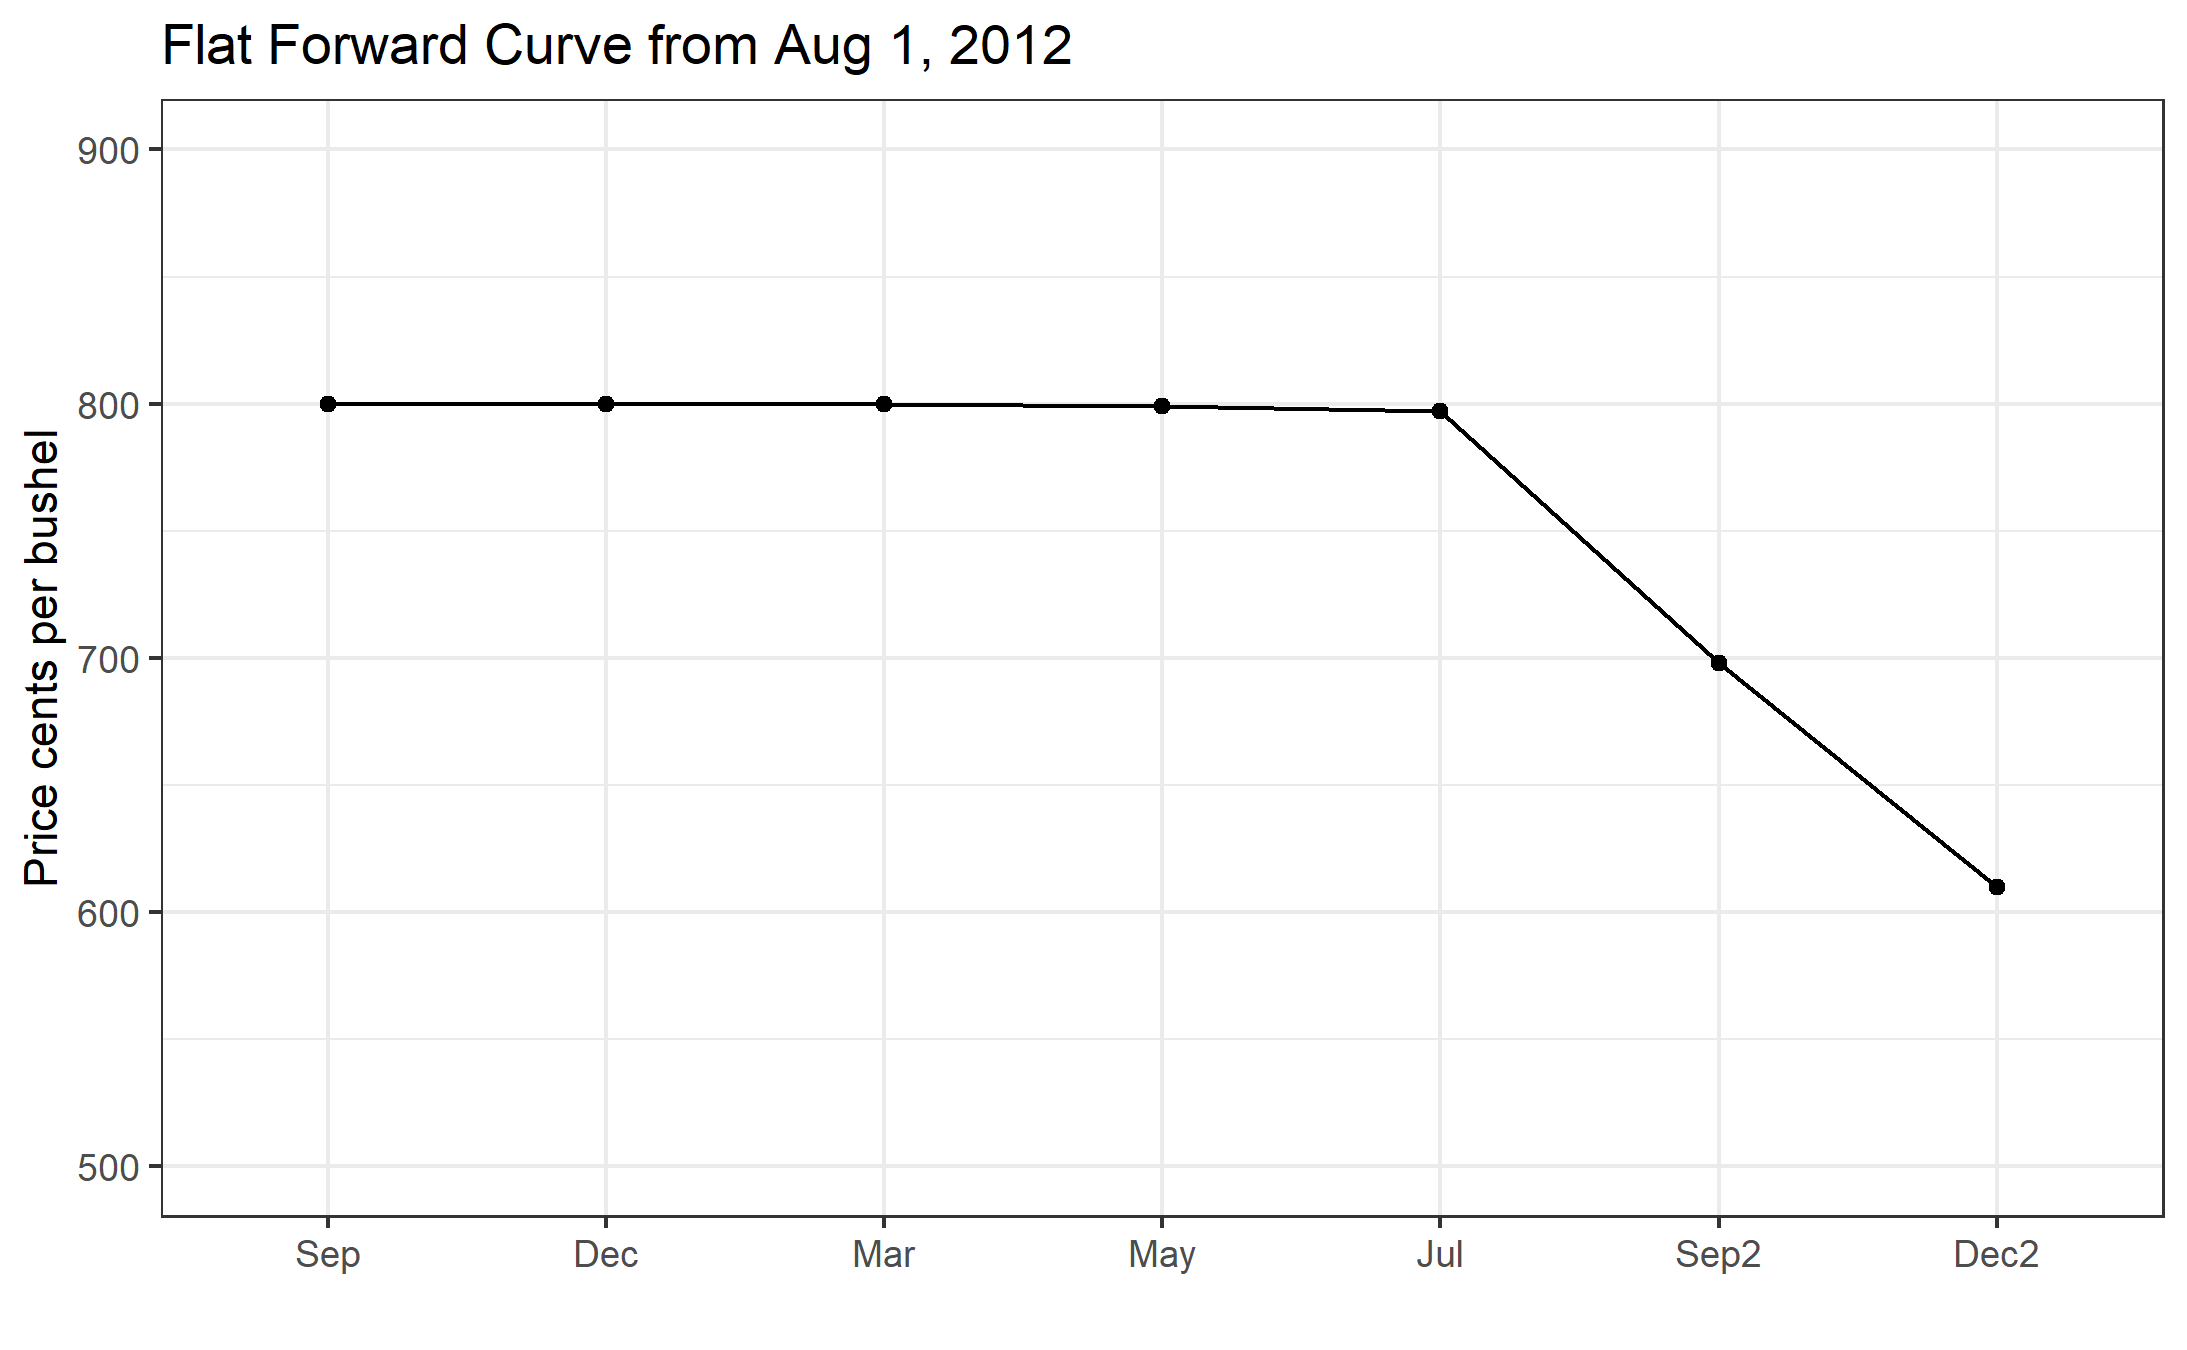
\includegraphics{assets/PricesSpaceTime-flat-8-01-2012.png}

Now, just to illustrate how the forward curve changed between August and
December 2012, the time in which harvest occurred and we learned exactly
how bad yields turned out to be, we show the forward curve on 12-03-2012
in figure 5.

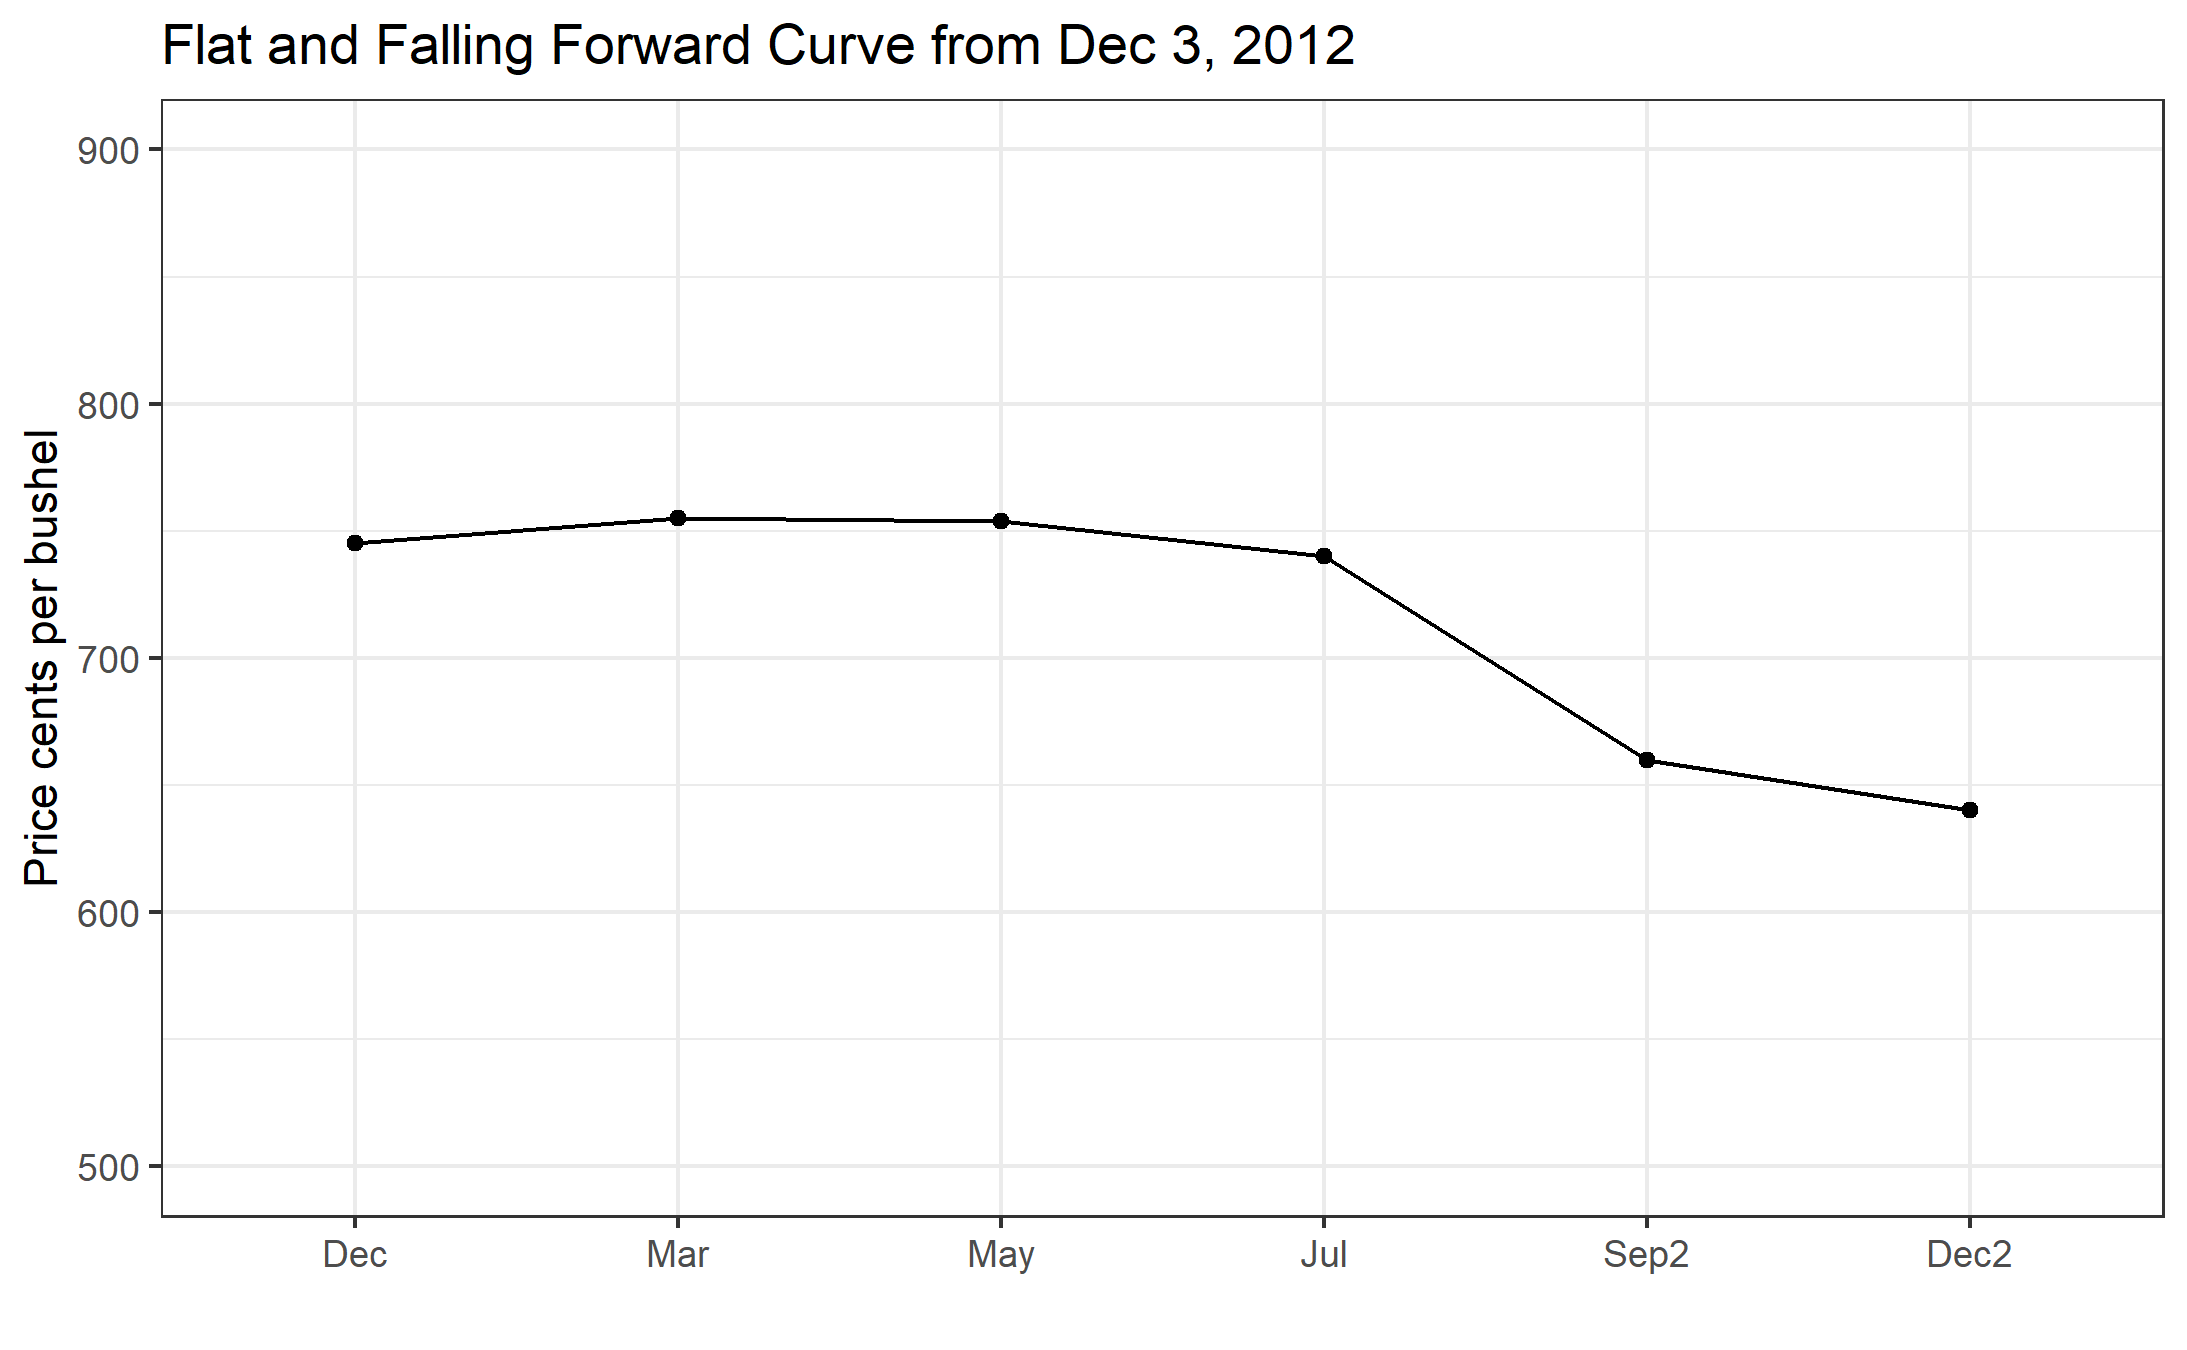
\includegraphics{assets/PricesSpaceTime-flat-12-03-2012.png}

\section{Forward Curve Cases with Hypothetical
Data}\label{forward-curve-cases-with-hypothetical-data}

When prices move up or down, the front end of the forward curve
generally is more responsive than the back end of the forward curve. We
will illustrate this with both increasing prices and decreasing prices.
The examples below show the first five contracts on the forward curve
plotted on four consecutive days of price changes in one direction. The
price data in these examples are hypothetical, but represent what
usually happens to the forward curve when prices increase or decrease.

\textbf{Prices Increasing}

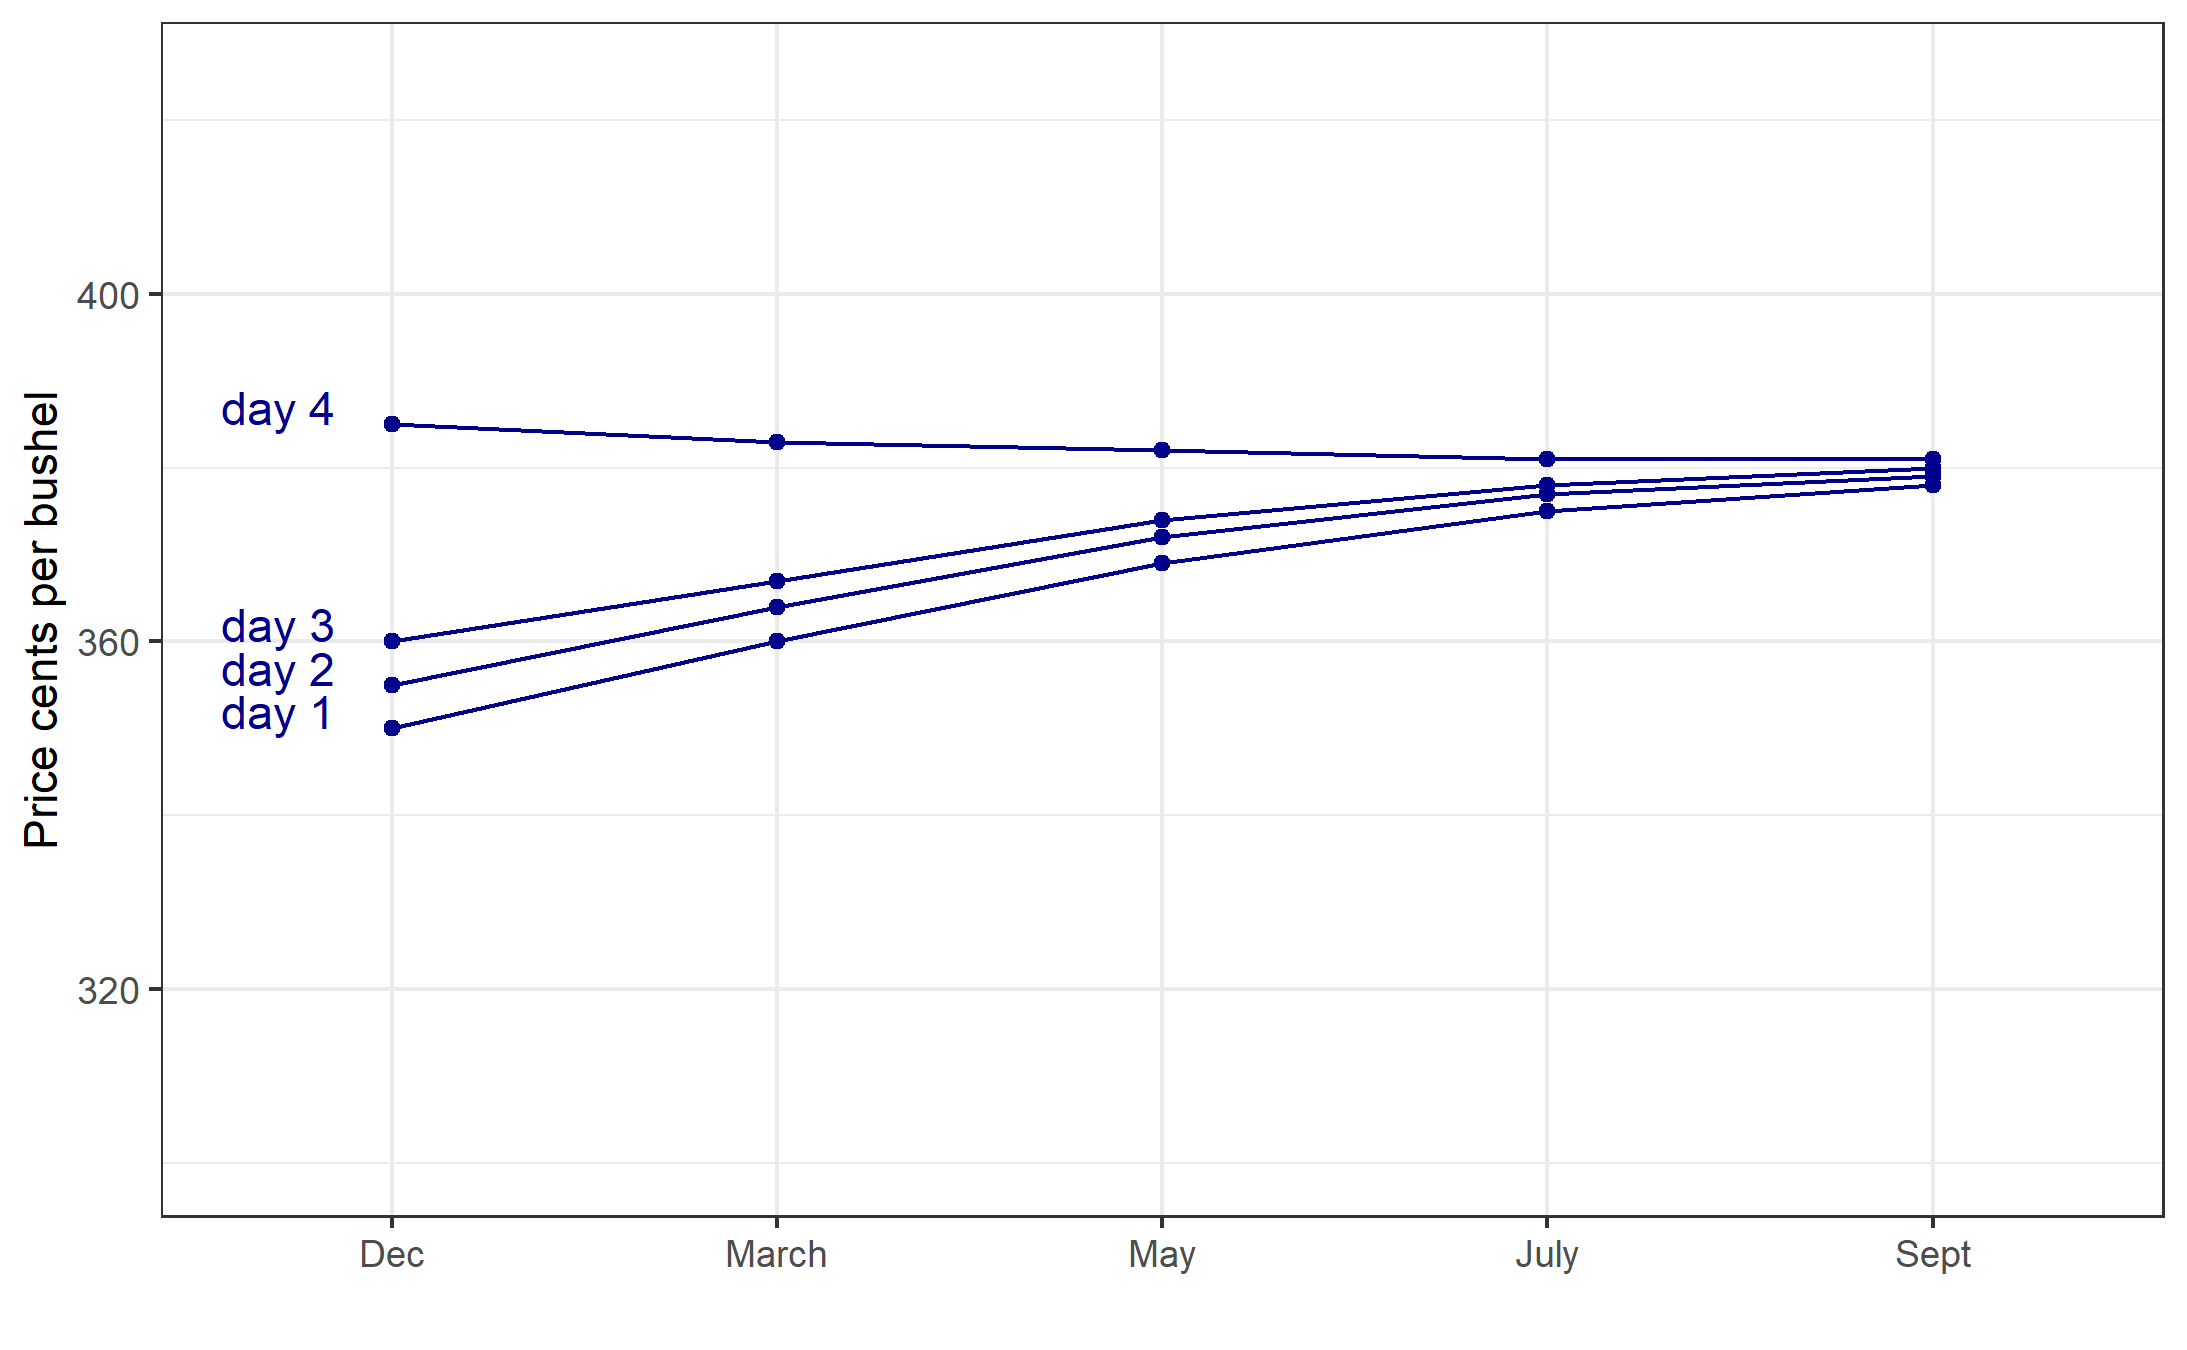
\includegraphics{assets/PricesSpaceTime-pricesincreasing-hyp.png}

Figure 6. Forward Curve with Prices Increasing, Contango to
backwardation

On day 1, the market is clearly in contango, as the forward curve is
upward sloped. As time moves from day 1 through day 4 prices are rising
each day, with the front end of the forward curve exhibiting the largest
changes each day. On day 4, prices have risen enough that the market is
now in backwardation with the front month higher than the first
deferred.

\textbf{Prices Decreasing}

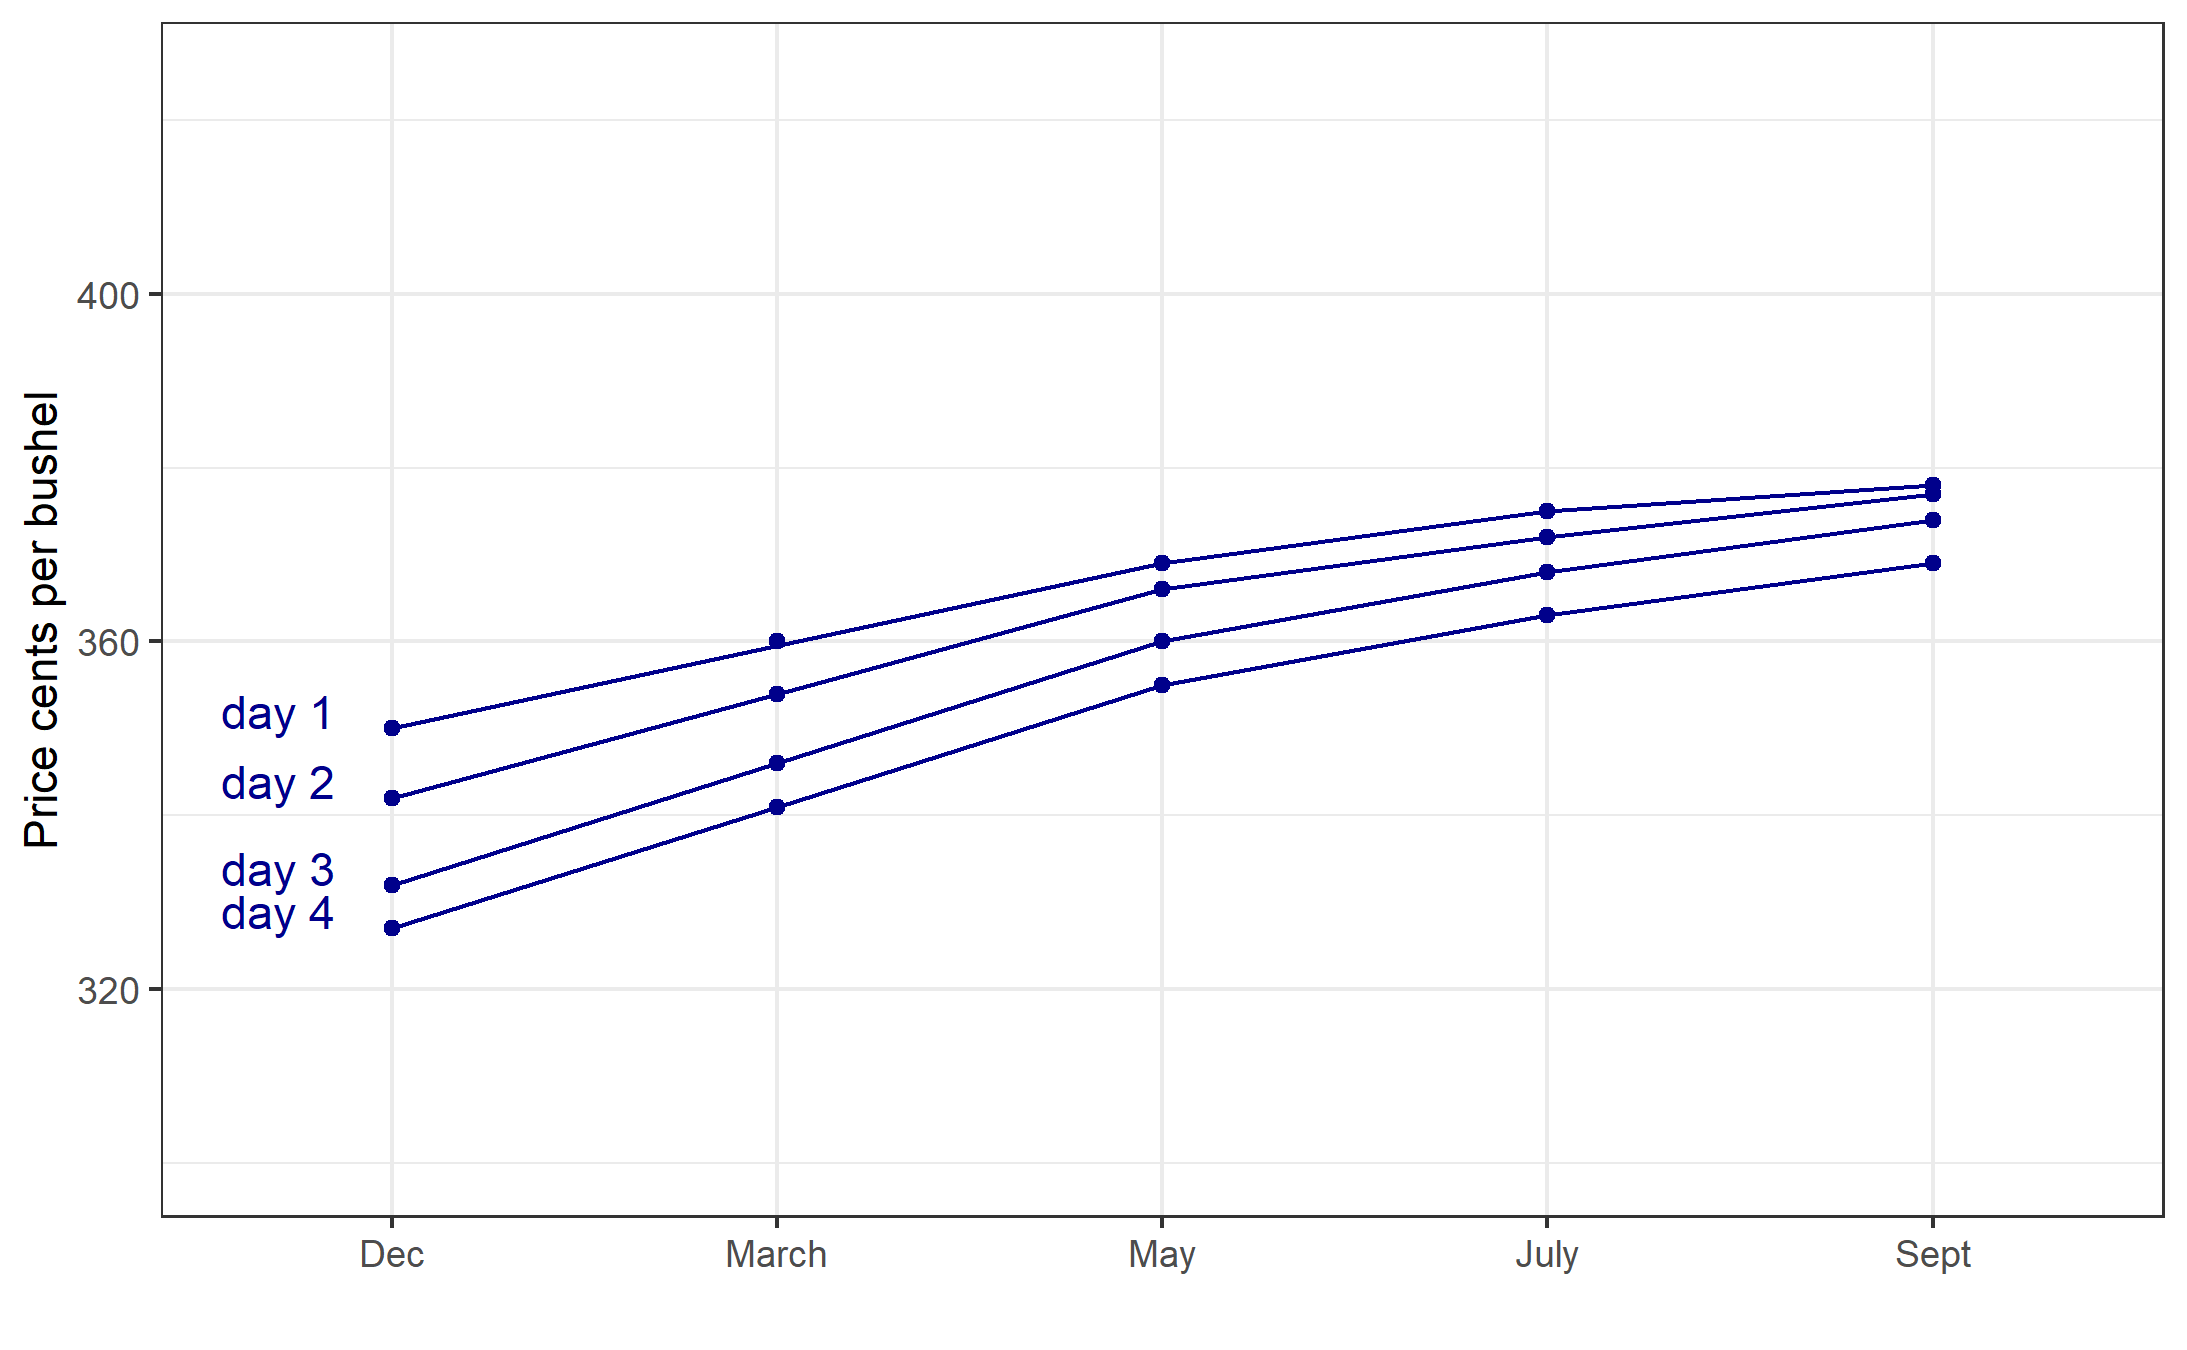
\includegraphics{assets/PricesSpaceTime-pricesdecreasing-hyp.png}

Figure 7. Forward Curve with Prices Decreasing

On day 1 the market is in contango in this example as well. As time
progresses from day 1 to day 4, prices are falling. From day 1 to day 3
the forward curve is getting steeper because price declines in Dec are
larger than the price declines in March. In turn, the price declines in
March are larger than the price declines in May, and do on. This
indicates that from day 1 to day 3, the market is not yet at full carry;
as prices are declining, the returns to storage keep increasing
(reflected by the steeper forward curve). From day 3 to day 4, however,
we can see that the market is at full carry because the price decline is
constant all the way up the forward curve. Even though prices continue
to fall, the market is already offering enough incentive to store to
cover storage costs, so the price differences between contracts cannot
widen any further.

\textbf{Some Caveats}

The effect of price changes on the shape of the forward curve as
described above is typically observed. However, there is nothing
requiring the market to react exactly this way, and there can be
fundamental changes in the market (perhaps a major demander of the
commodity reduces or increases consumption during a specific time of the
year) that affect parts of the forward curve more than others. This
could cause a larger price change in the middle or back end of the
forward curve. Usually though, the front end of the forward curve will
be more volatile than the back end of the forward curve as depicted in
figures 6 and 7.

\section{Financial Full Carry}\label{financial-full-carry}

We discussed at the beginning of this chapter that one of the costs of
storage to the farmer is the opportunity cost of money resulting from
deferring a sale, and how this makes it impossible to predict with
certainty any individual farmer's decision to store. However, there is a
concept called \textbf{financial full carry} that simply includes
interest costs and the premium charges on shipping certificates that we
discussed in Chapter 4.

\[Financial \text{  } Full \text{  } Carry  = ndays(\frac{i}{360}*F + P)\]

where \(ndays =\) the number of days between the first delivery day in
the nearby contract and the first delivery day in the deferred contract.
\(i =\) the three month LIBOR interest rate + 200 basis
points,\footnote{The CME Group uses simple interest to calculate the
  financial full carry in other contexts, so we adopt it here for our
  definition of financial full carry.} \(F =\) futures price, and
\(P =\) the current premium charge on shipping certificates. For
example, there are 90 days between delivery period of the December
contract and the delivery period of the March contract. If the LIBOR
rate is .3\% and financing costs are 200 basis points above LIBOR, the
corn futures price is \$3.50 per bushel, and the premium charge on
shipping certificates is 0.165 cents per bushel per day, then financial
full carry is:

\[Financial \text{  } Full \text{  } Carry = 90*(0.023/360*350 + 0.165 = 16.86 \text{ cents per bushel}) \]

Then financial full carry between the December contract and the March
contract would be 16.86 cents. It is called financial full carry because
in theory, the spread between the December and March contracts cannot be
wider than this amount. If it were wider, say 30 cents, then a storage
arbitrage would be possible. You could buy a December futures contract
and sell a March futures contract, take delivery of December contract,
receive the shipping certificate and hold it until March 1st at a cost
to you of 16.86 cents per bushel. Then use the shipping certificate to
deliver on your short March futures position. Your futures trades just
earned 30 cents, while holding the shipping certificate only cost 16.86
cents, leaving you with a profit of 13.14 cents per bushel.

Of course, the concept of financial full carry is really just a
benchmark. Most importantly, any individual's ability to capitalize on
the arbitrage in this example is predicated at the ability to borrow for
200 basis points over LIBOR. It is useful as a metric for how much of a
carry market we are in. Percent of full financial carry is a metric that
is widely followed
(\(\text{Percent of Full Carry } = 100*\frac{Futures \text{  } Calendar \text{  } Spread}{Full \text{  } Financial\text{  } Carry}\)),
because it gives similar information as the shape of the forward curve
in an easier metric to compare across time. In our example, percent of
full carry \(=100*30/16.86 = 177.94\%\) (remember this was an extreme
example to illustrate the potential for arbitrage).

\section{Calendar Spreads}\label{calendar-spreads}

The prior discussion has viewed the forward curve and returns to storage
from the perspective of a farmer or other who holds physical stocks of
grain. Speculators watch the price spread between futures contracts and
trade them to bet on whether or not returns to storage will increase or
decrease. These kinds of spreads are called \emph{Calendar Spreads} and
they are done by performing the following type of trade.

Following the same logic about expected scarcity of stocks, returns to
storage, and incentives for the market to bring stocks to the market, if
the price goes up, the nearby contract and front end of the forward
curve react the most strongly, deferred contracts will also go up, but
by a lesser amount. Likewise, if the price goes down, the nearby
contract will change the most; the deferred contract will also go down,
but less so.

So, a speculator places the following trades if they are bullish
(bearish):

\subsection{Bullish - think prices are going
up}\label{bullish---think-prices-are-going-up}

Buy Nearby: Dec 2017, Sell Deferred: March 2018

Then you are betting that prices in general will go up, but the nearby
will go up more than the deferred contracts. Any information event that
suggests supplies will become tighter should make prices go up in
general, and should reduce the incentive to store. Thus, making this a
profitable calendar spread trade.

\subsection{Bearish - think prices are going
down}\label{bearish---think-prices-are-going-down}

Sell Nearby: Dec 2017, Buy Deferred: March 2018

The opposite logic is at work here. You are betting that prices will go
down in general, but that the nearby will go down more than the deferred
contracts. Any information that suggests supplies will become more
plentiful should make prices go down in general, and should increase
incentives to store. Thus making the bearish calendar spread profitable.

To see today's forward curves in Corn and Soybeans visit
\href{https://mindymallory.shinyapps.io/ForwardCurves/}{here}.

\section{Price Variation Over Space}\label{price-variation-over-space}

Most of our time in this course has focused on what impacts futures
prices for commodities. However, a futures price represent the expected
future price of the commodity in a very specific location - the
locations that are `regular' for delivery. A location that is regular
for delivery is a location that is designated by the commodity exchange
where stocks of a commodity represented by a futures contract may be
delivered in fulfillment of the contract. This is where the spot, or
cash, price must come together, or converge, with the futures price.

\begin{figure}[H]

{\centering 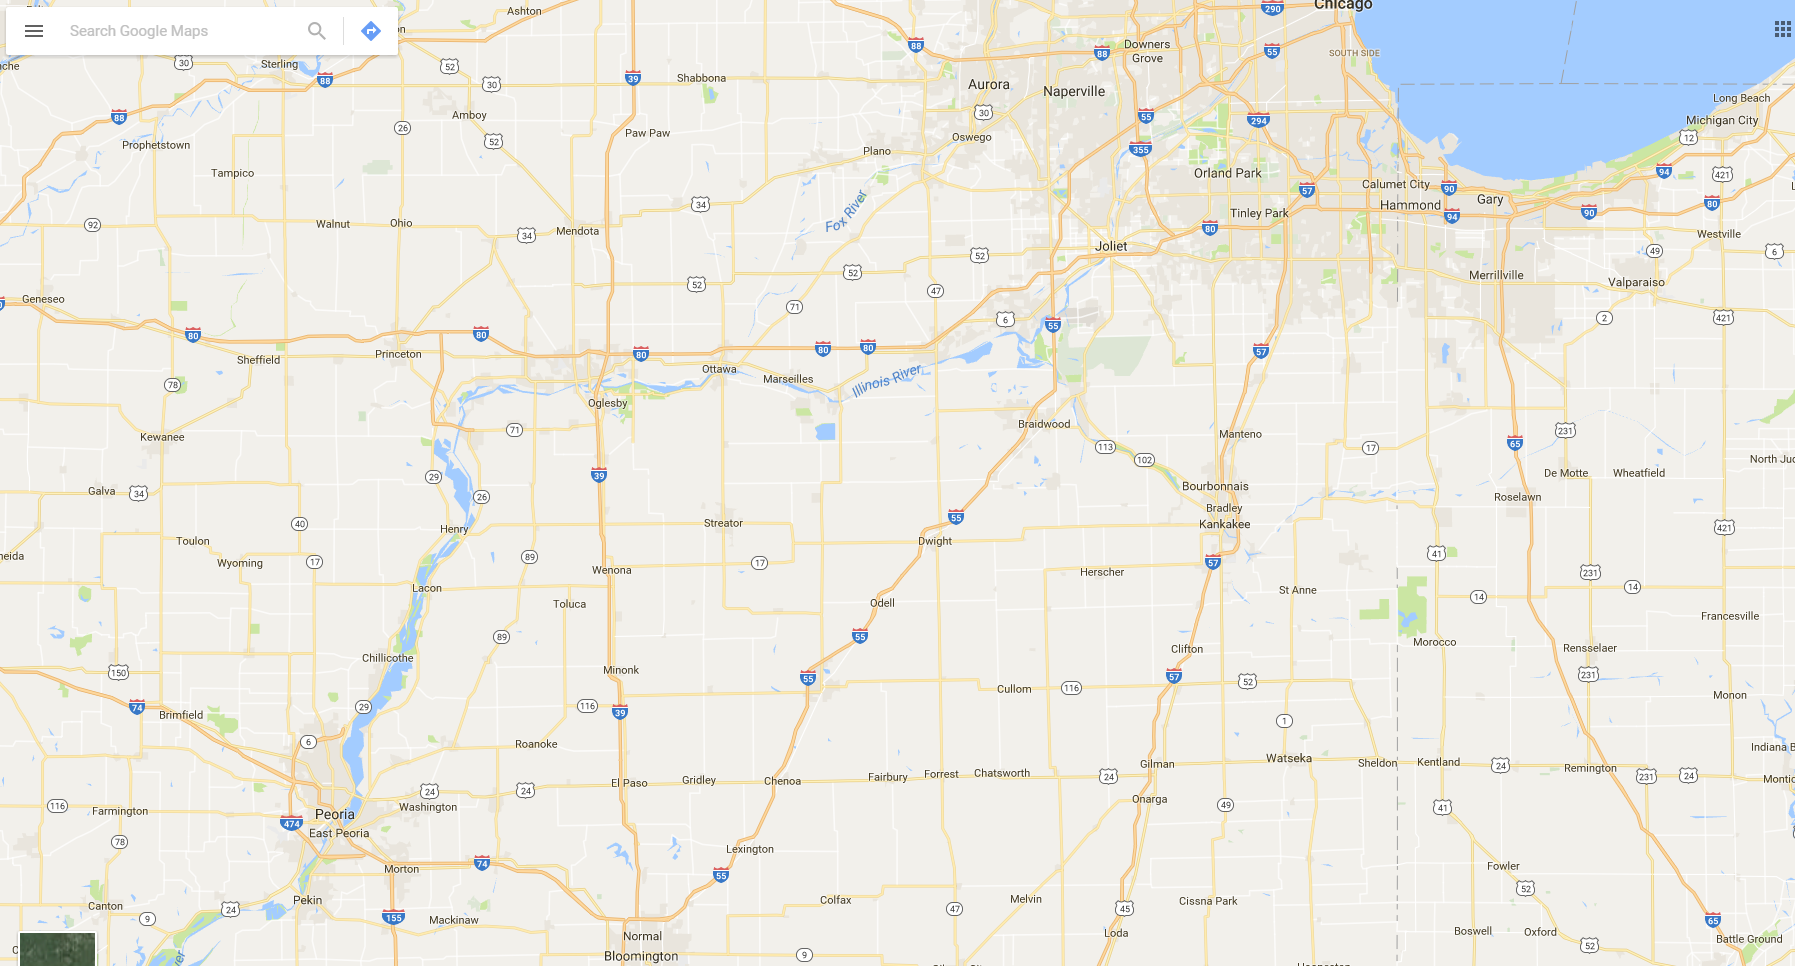
\includegraphics{images/IL-River.png}

}

\caption{Figure 11. Delivery Locations for Corn and Soybeans are Mostly
Along the Illinois River Between Chicago and Peoria, IL}

\end{figure}%

(Source \href{https://www.google.com/maps}{Google Maps})

\begin{figure}[H]

{\centering 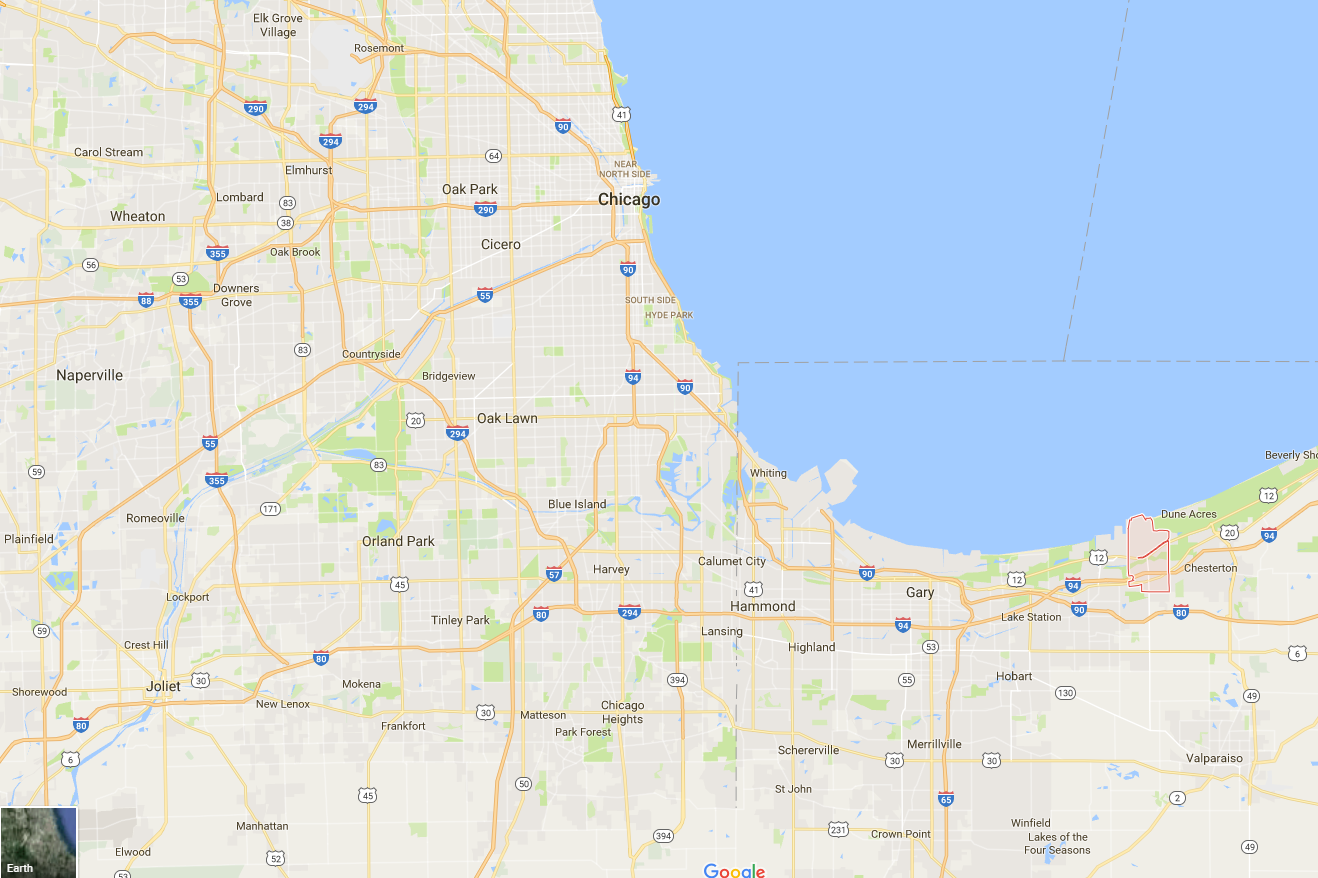
\includegraphics{images/Burns-Harbor.png}

}

\caption{Figure 12. Delvery Location at Burns Harbor, IN}

\end{figure}%

(Source
\href{https://www.google.com/maps/place/Burns+Harbor,+IN/@41.740398,-87.7248706,10.5z/data=!4m5!3m4!1s0x8811bc3712ab828d:0x98301a46014d10b5!8m2!3d41.6258708!4d-87.1333676}{Google
Maps})

Since the price of the futures contract is represents the expected
future price only at these locations (technically whichever is cheapest
to deliver) then the degree to which the futures price is indicative of
the expected future spot price at locations far from Northern Illinois
can vary.

Throughout the rural U.S., grain elevators, ethanol plants, soybean
crushers, feed yards and biodeisel manufacturers dot the landscape every
few miles. These entities buy essentially all of the grain and oilseed
crop that is not used on-farm for livestock feeding. They post bids to
buy every day they are open. They offer to buy as a cash sale, or on
forward contract for delivery one to three months ahead. In the case of
the forward contract, the farmer will go in to the elevator and sign a
contract to deliver a specific number of bushels within a specified
window of time. Usually, the prices quoted by grain elevators and other
prices is relative to the futures contract price, or basis.

In figure 13 the elevators around Champiagn, IL are shown.

\begin{figure}[H]

{\centering 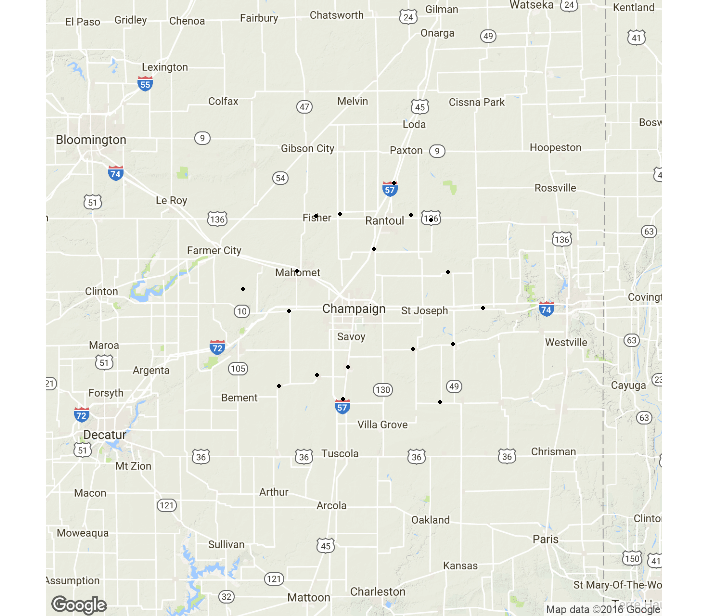
\includegraphics{images/Champaign-Elevators.png}

}

\caption{Figure 13. Elevators Around Champaign, IL}

\end{figure}%

Depending on how far the location is from the Illinois river, this
difference may be large, but still the futures price is the reference
point. The basis is often quoted as `over' or `under' the futures price.
For example, an elevator might post bids to buy for \(-27\) cents. This
means \(27\) cents under the futures price. A bid of \(31\) would be
read as \(31\) cents over the futures price.

\section{Definition of Basis}\label{definition-of-basis}

Basis is always defined as Spot Price minus Futures price.

\[Basis = Spot - Futures\]

Basis reflects the price differential over space relative to the futures
price. Basis is influenced by

\begin{itemize}
\tightlist
\item
  Transportation Costs
\item
  Local Supply and Demand Conditions
\item
  Interest and Storage Charges (this reflects that there is also a small
  time component as well as spatial)
\item
  Other Handling, Shipping and other Costs
\end{itemize}

Transportation costs are built into basis because large users of grain
are not necessarily located in large production region. E.g., cattle
feed yards in Western Kansas and Nebraska; Chickens in the South; and
Hogs in North Carolina. Grain is shipped by rail and/or truck to
locations across the country. Areas of grain surplus generally have a
negative basis, the spot price is less than the futures. Areas of grain
deficit generally have a positive basis, the spot price is greater than
the futures.

Local supply and demand conditions are also important. Occasionally,
there will be localized production problems. The biggest recent example
comes from the demand side, however. The expansion in ethanol production
in the U.S. was felt greatest in Iowa. As literally billions of gallons
of capacity in ethanol production came online in Iowa, the corn basis
was affected. With additional large consumers of corn located throughout
Iowa, there was more localized demand for corn. The ethanol plants and
grain elevators had increased localized competition, and local basis
bids started to rise between 2005 and 2010.

\section{Terminology}\label{terminology}

Farmers and grain handlers alike watch the basis closely, so discussion
of changes in the basis is common. When the basis is increasing, in most
cases that means becoming `less negative', we say the basis is
\textbf{stregthening}. When the basis is decreasing, or becoming `more
negative', we say the basis is \textbf{weakening}.

\bookmarksetup{startatroot}

\chapter{Balance Sheet Analysis}\label{balance-sheet-analysis}

{Interested in more? Please let me know by}
\href{https://forms.gle/Q3VByCQZHjfQSy9D7}{taking the survey}!

\textbf{Highlights}

\begin{itemize}
\tightlist
\item
  Balance sheet analysis is the most important tool for
  fundamentals-based price forecasting.
\item
  This chapter covers the format all balance sheets take, and introduces
  the USDA WASDE balance sheet.
\item
  This chapter shows what affects each row of the balance sheet.
\item
  This chapter provides a timeline of when the rows of a balance sheet
  can be updated.
\end{itemize}

\textbf{Check Your Understanding}

\begin{itemize}
\tightlist
\item
  Do you know which cells in the balance sheet must be estimated by the
  USDA and which can be calculated from other cells in the table?
\end{itemize}

Fundamental analysis is an assessment of price based on underlying
supply and demand factors. Focusing on changes in the relationship
between supply and demand allows one to calibrate an informed opinion of
the value of the commodity. The main role of the market is to find the
value at which supply equals demand - or in other words, the value that
`clears the market'. The estimated `fundamental value' is simply a
forecast, or expectation of, the market clearing price. The goal of any
forecasting exercise is to compare the forecast (estimated fundamental
value) to the current market price and make decisions accordingly.

If your forecast is above the current market price, that is bullish
because your forecast implies the market is undervaluing the commodity -
an opportunity to buy low and sell high! If your forecast is below the
current market price, that is bearish because your forecast implies the
market is overvaluing the commodity - an opportunity to sell high and
buy low! This, of course, only works if your forecast is correct, that
is, the market eventually agrees and moves into line with your forecast.

\section{Supply and Demand}\label{supply-and-demand}

Conducting fundamental analyses involves taking into account all the
factors that determine supply, demand, and ultimately, prices. For grain
markets there are basically two supply models to keep in mind:
preplanting and post planting. Below we display both.

\begin{figure}[H]

{\centering 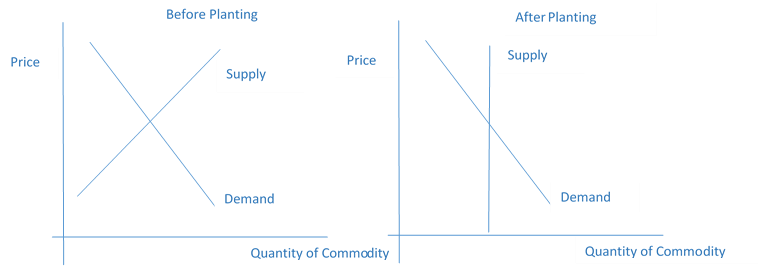
\includegraphics{images/Ch3.1.png}

}

\caption{Figure 1. Supply and Demand Model of a Commodity Before and
After Planting}

\end{figure}%

The intuition here is simply that before planting, the final supply for
the crop can be affected by farmers changing their intentions about how
many acres to plant. Once the crop has been planted, supply is
essentially fixed, except for the uncertainty that remains due to
realized yields. To summarize, things that affect the supply of a
commodity are outlined below.

\textbf{Supply is Affected by:}

\begin{itemize}
\item
  Acreage

  \begin{itemize}
  \tightlist
  \item
    Prices of crops competing for acreage
  \item
    Pre-Plant Weather
  \end{itemize}
\item
  Yield

  \begin{itemize}
  \tightlist
  \item
    Post-Plant Weather
  \end{itemize}
\item
  Government Policies
\end{itemize}

\begin{description}
\item[Acreage]
Before planting, farmers plan how much acreage to devote to each
commodity, thus determining the baseline expected production level.
Before summer weather is revealed, expected production is simply
\texttt{Acreage\ X\ Trend\ Yield}. In the Corn Belt, where planting
decisions amount to deciding how to divide acres between corn and
soybeans, their relative prices play a large role in the farmer's
decision. If futures prices indicate planting soybeans will be more
profitable than planting corn, farmers will plan to devote more acres
than usual to soybeans, for example. Weather can be an important
determinant of acreage decisions as well. The most ardent planting
intentions of a farmer can be derailed by persistent wet weather. An
unusually rainy planting season can reduce planted acres from
intentions. Before the crop is actually in the ground, the supply of
grain is relatively elastic.
\item[Yield]
After the crop is planted supply is quite inelastic, but there is still
considerable uncertainty related to how much the crop will yield; this
is largely determined by weather during the growing season.
\item[Government Policies]
The government has been heavily involved in Agriculture in the United
States since the great depression of the 1930's. There have been
programs that guarantee a minimum price, programs that guarantee minimum
revenue, and various incarnations of crop insurance programs.
Occasionally these favor the production of one type of crop over
another. When this happens, farmers predictably respond by planting more
of the crop treated more favorably by the program.
\end{description}

\textbf{Demand is Affected by:}

\begin{itemize}
\tightlist
\item
  Consumer Income
\item
  Exchange Rates
\end{itemize}

\begin{description}
\item[Consumer Income]
This one is straight from economics 101. When people have more money,
they will spend it on goods. This means increased demand for commodities
and their derived products. This includes foreign income, since exports
are a big component of demand for commodities in the United States.
Rising incomes usually means rising consumption of meat, which increases
the demand for commodities like corn, soybeans, and even wheat that are
used as animal feed.
\item[Exchange Rates]
Exchange rates also affect demand through their influence on exports.
For example, if the U.S. dollar is weak, then consumers in other
countries can buy dollars cheaply - giving them more purchasing power
for goods denominated in dollars.
\end{description}

\section{Balance Sheet}\label{balance-sheet}

Most fundamental analyses rely on maintaining balance sheets of a
commodity for a country, region, or the world. The approach is to
maintain a careful accounting of how much supply exists and how much of
the commodity has been used. Then through various means we will explore
later, one arrives at a price that is expected to ration remaining
supplies across competing uses.

\subsection{The Marketing Year and Balance Sheet Forecasting
Schedule}\label{the-marketing-year-and-balance-sheet-forecasting-schedule}

Balance sheet analysis is often organized by marketing year. Since
production happens once per year, the marketing year is defined to begin
in the first month the commodity is harvested and ends with the
following year's harvest. The table below makes note the month on which
marketing years begin for several crops.

\begin{longtable}[]{@{}
  >{\raggedright\arraybackslash}p{(\columnwidth - 2\tabcolsep) * \real{0.3077}}
  >{\raggedright\arraybackslash}p{(\columnwidth - 2\tabcolsep) * \real{0.6923}}@{}}
\caption{Table 1. Beginning of Marketing Year by Crop. (Source
\href{http://www.nass.usda.gov/Publications/National_Crop_Progress/}{NASS
Timetables})}\tabularnewline
\toprule\noalign{}
\begin{minipage}[b]{\linewidth}\raggedright
Crop
\end{minipage} & \begin{minipage}[b]{\linewidth}\raggedright
Beginning of Marketing Year - First Month of Harvest
\end{minipage} \\
\midrule\noalign{}
\endfirsthead
\toprule\noalign{}
\begin{minipage}[b]{\linewidth}\raggedright
Crop
\end{minipage} & \begin{minipage}[b]{\linewidth}\raggedright
Beginning of Marketing Year - First Month of Harvest
\end{minipage} \\
\midrule\noalign{}
\endhead
\bottomrule\noalign{}
\endlastfoot
Corn & September \\
Soybeans & September \\
Spring Wheat (Chicago) & August \\
Winter Wheat (KC) & July \\
\end{longtable}

Forecasting supply and demand for any given marketing year begins well
before harvest - nearly a year in advance, in fact. Table 2 below
follows the typical forecasting schedule with the 2017/2018 marketing
year. Note that is for the marketing year that begins with harvest in
September of 2016.

\begin{longtable}[]{@{}
  >{\raggedright\arraybackslash}p{(\columnwidth - 2\tabcolsep) * \real{0.1096}}
  >{\raggedright\arraybackslash}p{(\columnwidth - 2\tabcolsep) * \real{0.8904}}@{}}
\caption{Table 2: Forecasting Calendar for 2017/2018 Marketing
Year}\tabularnewline
\toprule\noalign{}
\begin{minipage}[b]{\linewidth}\raggedright
Timeline
\end{minipage} & \begin{minipage}[b]{\linewidth}\raggedright
Forecasting Focus
\end{minipage} \\
\midrule\noalign{}
\endfirsthead
\toprule\noalign{}
\begin{minipage}[b]{\linewidth}\raggedright
Timeline
\end{minipage} & \begin{minipage}[b]{\linewidth}\raggedright
Forecasting Focus
\end{minipage} \\
\midrule\noalign{}
\endhead
\bottomrule\noalign{}
\endlastfoot
Fall 2016 & The first forecasts of supply and use based on , \emph{trend
forecasts}, \emph{recent history}, \emph{economic relationships} \\
Spring 2017 & Update supply forecasts based on USDA acreage surveys. \\
Summer 2017 & Update supply forecasts based on weather and USDA crop and
stocks reports \\
Fall 2017 & Update supply forecasts as yield uncertainty is resolved
through harvest reports and USDA production reports \\
- Summer 2018 & Continue to update supply forecasts based on USDA
production revisions, southern hemisphere production, stocks, and use
reports. \\
\end{longtable}

\subsection{Southern Hemisphere
Production}\label{southern-hemisphere-production}

Production of corn, soybeans, and other commodities in the southern
hemisphere (most notably in Brazil and Argentina) has grown rapidly over
the last ten to fifteen years, and has impacted global commodity markets
tremendously. Since southern hemisphere production occurs in the middle
of marketing years organized by northern hemisphere harvest, there is an
uncertain additional supply that must be forecast and updated to keep an
accurate global balance sheet.

\subsection{Uncertainty}\label{uncertainty}

Even careful accounting of supply and demand factors that make up the
balance sheet leaves a tremendous amount of uncertainty in the market.
Demand can be difficult to forecast, and can sometimes change
dramatically. The USDA keeps careful track of stocks, but we only get
stocks estimates once a quarter. Between \emph{Grain Stocks} reports
there is always a great deal of speculation as to the pace of
consumption and whether we are eating into stocks at a faster or slower
pace than expected. Analysts talk about whether the market is on pace to
achieve the forecast level of ethanol crush, soybean crush, or exports.
Surprises in any of these components can lead to rapid corrections in
the commodity markets.

\subsection{Balance Sheet Format}\label{balance-sheet-format}

Here we discuss the common format balance sheets for any commodity have
in common. Then we talk about the components of specific balance sheets
for corn and soybeans.

\begin{longtable}[]{@{}ll@{}}
\caption{Table 3. Balance Sheet for a General Commodity}\tabularnewline
\toprule\noalign{}
Stocks and Use & \\
\midrule\noalign{}
\endfirsthead
\toprule\noalign{}
Stocks and Use & \\
\midrule\noalign{}
\endhead
\bottomrule\noalign{}
\endlastfoot
Beginning Stocks & \\
+ Production & \\
+ Imports & \\
\textbf{= Total Supply} & \\
Domestic Consumption & \\
+ Exports & \\
+ Residual & \\
\textbf{= Total Consumption (Use)} & \\
\textbf{Ending Stocks = Total Supply - Total Consumption} & \\
\end{longtable}

Since the USDA makes regular reports on the balance sheet for
commodities (the WASDE reports described in Chapter 2), most conducing
private analyses with balance sheets use the USDA categories so that the
USDA estimates can be taken as a benchmark. The supply side (Stocks) is
relatively straightforward. Total stocks for the marketing year will be
beginning stocks, the portion of last year's stocks that were not used
up during the previous marketing year, plus this year's production, plus
any imports of the commodity. Summing these three reveals the total
amount of the commodity available for use during the marketing year.

\begin{itemize}
\tightlist
\item
  Beginning Stocks: Some production from the previous year usually
  remains into the next crop season. Carryover stocks function as a
  buffer against current year yield uncertainty. For example, if
  carryover stocks are high and current year yield is expected to be
  below trend, the market price may fall in response but modestly.
  However, if carryover stocks are low - resulting from several years of
  below trend production and strong demand - then an expected yield
  below trend will likely cause a volatile rise in prices.
\end{itemize}

: Table 4. Recent USDA WASDE Balance Sheet for Corn

\begin{verbatim}
Response [https://downloads.usda.library.cornell.edu/usda-esmis/files/3t945q76s/dv140m16d/jm215h19t/latest.xls]
  Date: 2024-10-23 19:51
  Status: 200
  Content-Type: application/vnd.ms-excel
  Size: 326 kB
<ON DISK>  C:\Users\mindy\AppData\Local\Temp\RtmpwHUUdW\file694c3a7b22a2.xls
\end{verbatim}

\begin{table}
\centering
\begin{tabular}{l|r|r|r|r}
\hline
CORN & 2018/19 & 2019/20 Est. & 2020/21 Proj. Prev & 2020/21 Proj.\\
\hline
 &  &  &  & \\
\hline
\em{Million Acres} & \em{} & \em{} & \em{} & \em{}\\
\hline
Area Planted & 88.90 & 89.70 & 90.8 & 90.8\\
\hline
Area Harvested & 81.30 & 81.30 & 82.5 & 82.5\\
\hline
\em{Bushels} & \em{} & \em{} & \em{} & \em{}\\
\hline
Yield per Harvested Acre & 176.40 & 167.50 & 172.0 & 172.0\\
\hline
\em{Million Bushels} & \em{} & \em{} & \em{} & \em{}\\
\hline
Beginning Stocks & 2140.00 & 2221.00 & 1919.0 & 1919.0\\
\hline
Production & 14340.00 & 13620.00 & 14182.0 & 14182.0\\
\hline
Imports & 28.00 & 42.00 & 25.0 & 25.0\\
\hline
\textbf{Supply, Total} & \textbf{16509.00} & \textbf{15883.00} & \textbf{16127.0} & \textbf{16127.0}\\
\hline
Feed and Residual & 5429.00 & 5903.00 & 5650.0 & 5650.0\\
\hline
Food, Seed \& Industrial 2/ & 6793.00 & 6282.00 & 6375.0 & 6375.0\\
\hline
Ethanol \& by-products 3/ & 5378.00 & 4852.00 & 4950.0 & 4950.0\\
\hline
\textbf{Domestic, Total} & \textbf{12222.00} & \textbf{12185.00} & \textbf{12025.0} & \textbf{12025.0}\\
\hline
Exports & 2066.00 & 1778.00 & 2550.0 & 2600.0\\
\hline
\textbf{Use, Total} & \textbf{14288.00} & \textbf{13963.00} & \textbf{14575.0} & \textbf{14625.0}\\
\hline
Ending Stocks & 2221.00 & 1919.00 & 1552.0 & 1502.0\\
\hline
\textbf{Avg. Farm Price (\$/bu)  4/} & \textbf{3.61} & \textbf{3.56} & \textbf{4.2} & \textbf{4.3}\\
\hline
\end{tabular}
\end{table}

(source: February 2021 USDA WASDE Report)

The balance sheet for corn follows the same generic patter, but we can
be a bit more specific with the use categories since we know what the
major use categories are for any given commodity. The use components are
as follows:

\begin{itemize}
\tightlist
\item
  Feed and Residual: A large portion of the corn crop is used as feed
  for livestock (cattle, pigs, poultry).
\item
  Food, Seed, and Industrial: Corn is used to make tortilla chips, high
  fructose corn syrup, edible oil and other food items. A portion of the
  crop is grown specifically as seed for the next years crop. There are
  some industrial uses for components of processed corn. Those are
  grouped in this category as well.
\item
  Ethanol production also demands a significant amount of corn, so much
  that it gets its own line in the balance sheet. Note, however, that it
  is technically part of the Food, Seed, and Industrial category.
\item
  The final use category is export. Corn grown in the United States is
  consumed around the globe, and strength or weakness in the export
  market is a carefully component of demand.
\end{itemize}

: Table 5. Recent USDA WASDE Balance Sheet for Soybeans

\begin{table}
\centering
\begin{tabular}{l|r|r|r|r}
\hline
SOYBEANS & 2018/19 & 2019/20 Est. & 2020/21 Proj. Prev & 2020/21 Proj.\\
\hline
\textbf{} & \textbf{} & \textbf{} & \textbf{ \vphantom{2}} & \textbf{}\\
\hline
Million Acres &  &  &  \vphantom{1} & \\
\hline
 &  &  &  & \\
\hline
Area Planted & 89.20 & 76.10 & 83.10 & 83.10\\
\hline
Area Harvested & 87.60 & 74.90 & 82.30 & 82.30\\
\hline
\em{Bushels} & \em{} & \em{} & \em{} & \em{}\\
\hline
Yield per Harvested Acre & 50.60 & 47.40 & 50.20 & 50.20\\
\hline
\em{Million Bushels} & \em{} & \em{} & \em{} & \em{}\\
\hline
 &  &  &  & \\
\hline
Beginning Stocks & 438.00 & 909.00 & 525.00 & 525.00\\
\hline
Production & 4428.00 & 3552.00 & 4135.00 & 4135.00\\
\hline
Imports & 14.00 & 15.00 & 35.00 & 35.00\\
\hline
\textbf{Supply, Total} & \textbf{4880.00} & \textbf{4476.00} & \textbf{4695.00} & \textbf{4695.00}\\
\hline
Crushings & 2092.00 & 2165.00 & 2200.00 & 2200.00\\
\hline
Exports & 1752.00 & 1682.00 & 2230.00 & 2250.00\\
\hline
Seed & 88.00 & 96.00 & 103.00 & 103.00\\
\hline
Residual & 39.00 & 9.00 & 22.00 & 22.00\\
\hline
\textbf{Use, Total} & \textbf{3971.00} & \textbf{3952.00} & \textbf{4555.00} & \textbf{4575.00}\\
\hline
Ending Stocks & 909.00 & 525.00 & 140.00 & 120.00\\
\hline
Avg. Farm Price (\$/bu)  2/ & 8.48 & 8.57 & 11.15 & 11.15\\
\hline
Total &  &  &  & \\
\hline
\end{tabular}
\end{table}

(source: February 2021 USDA WASDE Report)

For soybeans, stocks are comprised of beginning stocks, production, and
imports, just as they were for the general balance sheet and the corn
balance sheet. The use side, contains items specific to soybeans:

\begin{itemize}
\tightlist
\item
  Crush: The amount of raw soybeans that are processed into soybean oil
  and soybean meal. Soybean oil is used predominately as edible oil; it
  also is used to make bio-diesel in modest quantities.
\item
  Food, Seed, and Industrial: We saw this category in the corn balance
  sheet. The definition remains the same.
\item
  Exports: The United States exports a large quantity of soybeans to
  global buyers.
\end{itemize}

\section{Coming up with a Price}\label{coming-up-with-a-price}

Balance sheet forecasting is definitely as much art as it is science. It
involves keeping track of the rate of use of commodities to see how much
a need there will be to ration late in the marketing year while waiting
on harvest and new supplies. One should intuitively see that the
forecasted ending stocks is a measure of scarcity of the commodity and
therefore should be negatively related to price (i.e., tight ending
stocks go along with high prices). One needs to pin down the exact
nature of this relationship in order to form a meaningful forecast of
price from a commodity balance sheet. We will discuss this process in
more detail in a later chapter.

\section{Readings}\label{readings-2}

\begin{description}
\item[\href{http://farmdocdaily.illinois.edu/2015/02/balance-sheet-projections-for-2015-16-corn-marketing-year.html}{Balance
Sheet Projections for the 2015-16 Corn Marketing Year}]
This \emph{farmdoc daily} article was written in February of 2015. This
is well before spring planting of corn and soybeans in the United
States. However, farmers during this time are actively planning for
planting season - prepping equipment, fertilizing and preparing ground,
and buying seed. Good lays out the groundwork for early forecasts of the
2015/2016 marketing year balance sheet. This article is published two
days before the February 2015 WASDE report, and Good provides context
upon which market expectations for the WASDE report can be based upon.

Good, D.
``\href{http://farmdocdaily.illinois.edu/2015/02/balance-sheet-projections-for-2015-16-corn-marketing-year.html}{Balance
Sheet Projections for the 2015-16 Corn Marketing Year}.'' \emph{farmdoc
daily} (5):23, Department of Agricultural and Consumer Economics,
University of Illinois at Urbana-Champaign, February 9, 2015.
\item[\href{http://farmdocdaily.illinois.edu/2015/04/projecting-2015-16-corn-balance-sheet.html}{Projecting
the 2015-16 Corn Balance Sheet and Price Implications}]
In this reading Good and Irwin break down the USDA's April 9th WASDE
report and offer their own projections that differ slightly from the
USDA's projection that came out a week earlier. Pay close attention to
why their price estimate is higher than the USDA's.

Good, D., and S. Irwin.
``\href{http://farmdocdaily.illinois.edu/2015/04/projecting-2015-16-corn-balance-sheet.html}{Projecting
the 2015-16 Corn Balance Sheet and Price Implications}.'' \emph{farmdoc
daily} (5):70, Department of Agricultural and Consumer Economics,
University of Illinois at Urbana-Champaign, April 16, 2015.
\end{description}

\section{Exercises}\label{exercises-2}

\begin{enumerate}
\def\labelenumi{\arabic{enumi}.}
\item
  Copy and paste the corn and soybeans balance sheets into a
  spreadsheet.

  \begin{itemize}
  \tightlist
  \item
    In the cell next to \textbf{= Total Supply}, manually add the cells
    needed to reproduce the \textbf{`=Total Supply'} number.
  \item
    in the cell next to \textbf{= Total Consumption}, manually add the
    cells needed to reproduce the \textbf{= Total Consumption} number.
  \end{itemize}
\item
  If you were making a forecast in July 2015 for the 2014/2015 marketing
  year balance sheet, which columns (if any) should remain fixed? I.e.,
  they are already determined and do not need to be forecast.
\item
  If you were making a forecast in July 2015 for the 2015/2016 marketing
  year balance sheet, which columns (if any) should remain fixed?
\end{enumerate}

\bookmarksetup{startatroot}

\chapter{Price Reaction to USDA
Reports}\label{price-reaction-to-usda-reports}

{Interested in more? Please let me know by}
\href{https://forms.gle/Q3VByCQZHjfQSy9D7}{taking the survey}!

Some of the USDA reports contain very sensitive market information
causing market prices to adjust rapidly to new information about supply
and demand. Access to the contents of a market sensitive report would
result in the ability to perform `insider trading' and obtain nearly
risk-less profits. This activity is illegal, and the USDA's Interagency
Commodity Estimates Committees prepares the reports under lock-down
conditions where during the process of finalizing estimates of the
report's content, officials are locked in a secure area and not allowed
to leave until the report is made known to the public.

This chapter explores some history related to the compilation and
release of USDA reports, discusses how release times have evolved over
time, indicates some particular report releases that are more likely to
cause large and rapid price adjustments, and demonstrates this with a
few charts of transactions prices pre- and post-release of particularly
interesting recent days.

\section{History - ``The Great Data Leak of
1905''}\label{history---the-great-data-leak-of-1905}

This abundance of care can be traced to a particular event in history.
The details of which are recounted in a historical publication by the
NASS.

\begin{figure}[H]

{\centering 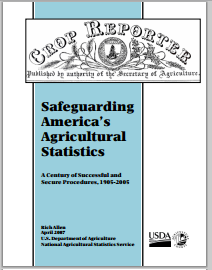
\includegraphics{images/NASS_History.png}

}

\caption{Figure 1: Safeguarding America's Agricultural Statistics: A
century of Successful and Secure Procedures}

\end{figure}%

Source:
\href{pdf-Readings/safegaurding-americas-agricultural-statistics.pdf}{NASS:
About Nass}

\begin{quote}
\section{Excerpt From Chapter 1}\label{excerpt-from-chapter-1}

The summary and release procedures for the USDA Bureau of Statistics'
reports in the early 1900s produced separate summary tabulations for
each data source available (up to six sources, in some cases)\ldots{} It
is also relevant that the release time for cotton reports in those years
was noon, Eastern Time, and that the commodity markets discontinued
trading for an hour starting at noon on release days. The original
procedures allowed the three people who had determined the final numbers
to go about their business, or even leave the building if they wished,
once a report's contents had been set.

In 1904 there were rumors about insider trading. As came to light later,
one of the three Bureau of Statistics people, E.S. Holmes, Jr., did have
an outside partner, a NewYork cotton trader named Louis Van Riper.
Shortly after an estimate was set, Holmes would meet Van Riper and tell
him what cotton estimate was going to be published. Van Riper would take
whatever market action would be most profitable based on the advance
information.

The scheme came to light following the cotton acreage report issued on
June 2, 1905. The three members met and adopted the state and national
figures to be published. After Holmes had sent his signal, one of the
other people who had worked on the report asked for reconsideration.
After further review, the figures to be published were revised. At that
point, the outside partner had already interpreted the original signal
and proceeded to place trades. The scheme came to light when Van Riper
charged in a telegram that a ``fraudulent'' report had been released. In
explaining why he thought this was a false report, he unwittingly
revealed that he had the information ahead of time. Evidently, Holmes'
outside partner had an overabundance of ego, but not a good balance of
common sense in going public with his story. (Allen 2007)
\end{quote}

This story is quite similar to the plot line of the 1980's movie,
\href{http://www.imdb.com/title/tt0086465/}{Trading Places}.\footnote{Anyone
  interested in a career in trading should watch this movie and then
  watch it again. You still hear references to the movie.} Where the
protagonists (Dan Aykroyd and Eddie Murphey) trick to antagonists, the
Duke Brothers by replacing the `Orange Juice Crop Report' that they
obtained illegally with a forged one that would cause exactly the
opposite price effect. They started buying before the report to profit
and Dan Aykroyd and Eddie Murphey start selling based on the correct
crop report information. The frenzy on the trading floor captures the
feeling of what happens during crop reports that move the market, even
if there is no longer trading on a physical floor as shown in the movie.

\section{Changing Report Release
Times}\label{changing-report-release-times}

Timing of report releases has important implications for the market
reaction as well. Figure 2 below provides a brief history of report
release times of major market sensitive reports.

\begin{figure}[H]

{\centering 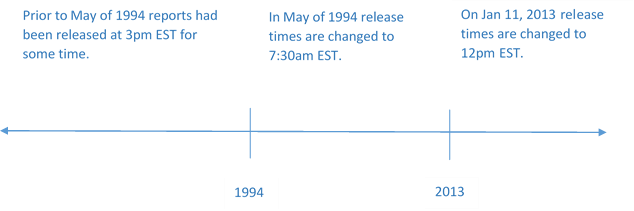
\includegraphics{images/NASS_release_timeline.png}

}

\caption{Figure 2: Timeline of Report Release Times}

\end{figure}%

Prior to 1994 most market sensitive USDA reports were released at 3pm
EST. This made sense from the USDA workflow perspective because it
allowed the lock-down to be enacted during normal working hours,
minimizing disruption of the analysts' regular lives. By the early 90's
releasing the report at this time became unpopular with market
participants. By releasing the report late in the afternoon in the U.S.
futures markets in other parts of the world could trade the USDA numbers
overnight before the U.S. market had a chance to react. Therefore price
discovery after reports was essentially shifted from Chicago to other
major exchanges across the world.

In May of 1994, the USDA shifted the release time to 8:30am EST. This
meant the report was released during regular business hours in the U.S.
and just one hour before trading begins on the U.S. futures exchange.
While clearly preferable to market participants in the U.S. this moved
the USDA's lockup time to overnight hours (Allen 2007).

By 2011, presumably due to the ability to trade electronically with high
speed, there was a desire for the futures market to be open and actively
trading at the time USDA reports were released. In this case, the
futures exchange acted first, expanding trading hours to an earlier
market open. Eventually, since futures market participants wanted it,
and because came with the added benefit of moving the beginning of the
lockup period from late night to early morning, the USDA began releasing
most reports at 12pm EST on January 11, 2013.

\section{Price Reactions}\label{price-reactions}

Market prices react strongly to USDA reports when the reports inject
significant and unanticipated information into the market. Some reports
are more likely than others to produce fireworks in terms of market
price.

\begin{longtable}[]{@{}
  >{\raggedright\arraybackslash}p{(\columnwidth - 4\tabcolsep) * \real{0.1509}}
  >{\raggedright\arraybackslash}p{(\columnwidth - 4\tabcolsep) * \real{0.0943}}
  >{\raggedright\arraybackslash}p{(\columnwidth - 4\tabcolsep) * \real{0.7484}}@{}}
\caption{Table 1: Reports most likely to cause significant movements in
market price}\tabularnewline
\toprule\noalign{}
\begin{minipage}[b]{\linewidth}\raggedright
Report
\end{minipage} & \begin{minipage}[b]{\linewidth}\raggedright
Dates
\end{minipage} & \begin{minipage}[b]{\linewidth}\raggedright
Reason
\end{minipage} \\
\midrule\noalign{}
\endfirsthead
\toprule\noalign{}
\begin{minipage}[b]{\linewidth}\raggedright
Report
\end{minipage} & \begin{minipage}[b]{\linewidth}\raggedright
Dates
\end{minipage} & \begin{minipage}[b]{\linewidth}\raggedright
Reason
\end{minipage} \\
\midrule\noalign{}
\endhead
\bottomrule\noalign{}
\endlastfoot
Grain Stocks & Quarterly & Information about scarcity or surplus of
supplies \\
Prospective Plantings & End of March & Acreage and therefore production
estimates \\
Planted Acres & End of June & Acreage and therefore production
estimates \\
WASDE & October & Some years the Oct report will contain significant
revisions from previous estimate \\
WASDE & January & Final production estimate for the preceding harvest.
Sometimes includes and unanticipated revision \\
Crop Progress Report & Weekly & Condition estimates. Only moves market
prices if significant deterioration associated with a drought or flood
occurs \\
\end{longtable}

\begin{description}
\item[Grain stocks]
Estimates only come out quarterly. Since the information about whether
we have a scarcity or surplus is a primary driver of price, and since we
only get this report four times per year, the stocks estimate can cause
significant adjustments in price.
\item[Prospective Planting and Planted Acres]
Reports give a baseline expectation about production for the coming
marketing year. Deviations from expectations or recent history will
cause rapid adjustments in price.
\item[WASDE]
The reports in October and January are relatively more likely to cause
rapid price adjustments than other months because in October the yield
estimates tend to become more precise and can involve significant
revisions from the previous month's estimate. Similarly, January report
contains finalized estimates of the crop production and in some cases
will involve unexpected revisions from previous estimates.
\item[Crop Progress]
These reports generally only move markets when crop conditions are
deteriorating rapidly due to drought or excess moisture. During years
with more typical weather, this report does not affect markets much
week-to-week.
\end{description}

\subsection{Some Examples of Recent Big Market
Reactions}\label{some-examples-of-recent-big-market-reactions}

Using the Best Bid Best Offer database from the CME Group's
\href{http://www.cmegroup.com/market-data/datamine-historical-data/}{DataMine}
we can examine historical intraday transaction prices (like what is
available streaming in real-time from Yahoo Finance or other sources).
These data are time-stamped to the second and allow the most accurate
and fine scale picture of futures market trading tick-by-tick.

Three examples come from the 2010 marketing year.

The June 30 Planted Acres report resulted in the market opening (at
8:30am EST) 15 cents higher than it closed the overnight trade just two
hours earlier. Ultimately it closed the day trading session 3.54
cents/bushel - 7.5\% or 25 cents higher than the most recent pre-report
price. Two put that into perspective, 25 cents that is an increase in
value of one futures contract of \$1,250, since future contracts are
specified for a quantity of 5,000 bushels.

Figure 2: Price of July 2010 corn on June 30, 2010 before and after the
release of Planted Acres Report

\includegraphics{11-PriceReactionto_files/figure-pdf/unnamed-chunk-1-1.pdf}

In the top panel of Figure 2 you can see that the time stamps indicate
those are transactions occurring in the overnight electronic market.
There is a break in the morning prior to 9:30 CST when trading begins in
the daytime session. It is in this period that the Planted Acres report
is released. The bottom panel only displays the daytime session, so that
you can see the trading action more clearly. Between 9:30am and about
10:15 the market trades in a 10 cent range.

The Oct 8th WASDE report caused the market to open limit up. The
exchange sets the maximum fluctuation a futures price can trade in a
given day. The value of the limit can change at the discretion of the
exchange with some advance notice. The report indicated a sharp drop in
forecasted yield for corn. This resulted in the ending stocks number for
the 2010/2011 marketing year forecast below 1 billion bushels with a
very low stocks to use ratio as well. The market reaction is show below
in Figure 3.

Figure 3: Price of December 2010 corn on October 8th, 2010 before and
after the release of the WASDE Report

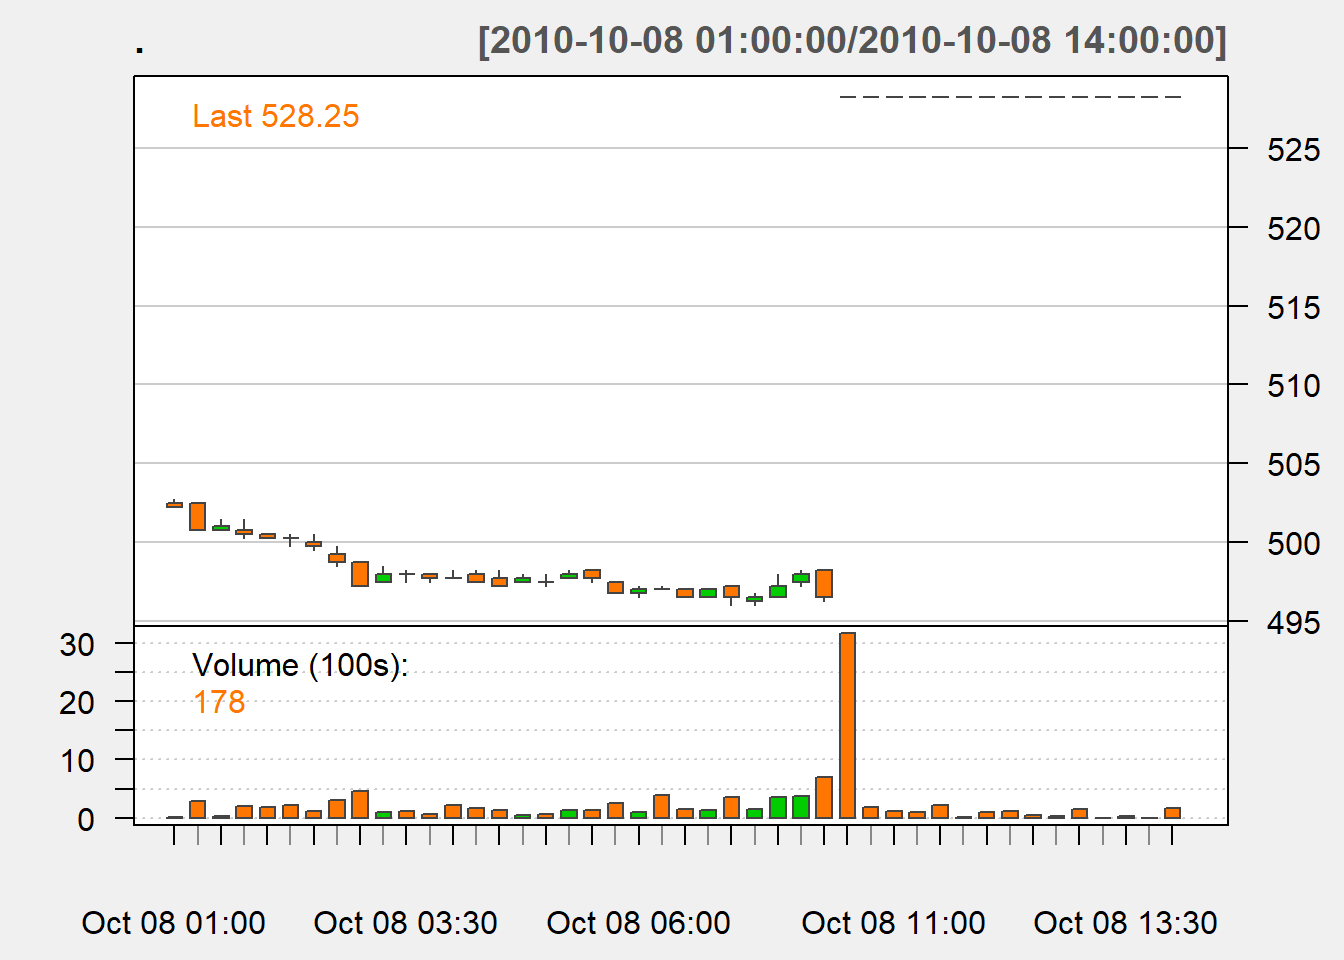
\includegraphics{11-PriceReactionto_files/figure-pdf/unnamed-chunk-2-1.pdf}

The flat line during the daytime trading session is apparent, resulting
from prices being locked at the limit during the entire trading day.

Figure 5: Price of May 2011 corn on March 31st, 2011 before and after
the release of the Planted Acres Report

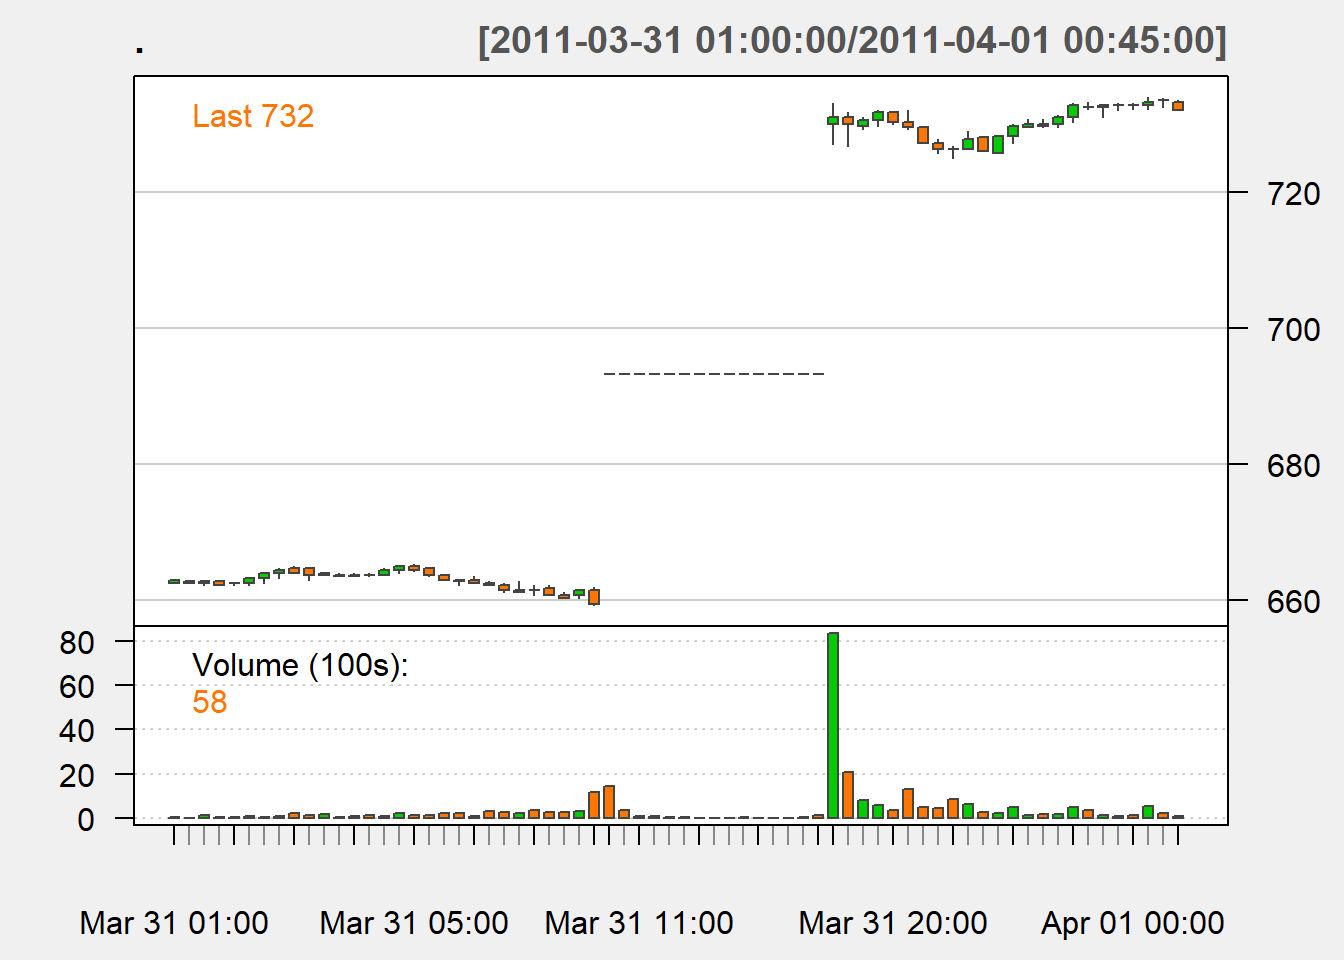
\includegraphics{11-PriceReactionto_files/figure-pdf/unnamed-chunk-3-1.pdf}

This report indicated that corn acreage was to be higher than previously
expected, but corn stocks were lower than expected. The stocks number
dominated the price direction strongly and the market traded limit up on
this day as well.

\section{Conclusions}\label{conclusions}

This chapter reviewed the history of report released by the USDA. We
noted a data leak in 1905 led the agency to consider security from an
early date - a important component of report production that persists to
this day. We also learned that the Prospective Plantings, Planted
Acreage, October WASDE, January WASDE, and Grain Stocks reports are the
most likely to produce rapid price adjustments in the market. Some
specific examples were given, and depicted through charts of transaction
prices.

\bookmarksetup{startatroot}

\chapter{Price Reaction to USDA
Reports}\label{price-reaction-to-usda-reports-1}

{Interested in more? Please let me know by}
\href{https://forms.gle/Q3VByCQZHjfQSy9D7}{taking the survey}!

Some of the USDA reports contain very sensitive market information
causing market prices to adjust rapidly to new information about supply
and demand. Access to the contents of a market sensitive report would
result in the ability to perform `insider trading' and obtain nearly
risk-less profits. This activity is illegal, and the USDA's Interagency
Commodity Estimates Committees prepares the reports under lock-down
conditions where during the process of finalizing estimates of the
report's content, officials are locked in a secure area and not allowed
to leave until the report is made known to the public.

This chapter explores some history related to the compilation and
release of USDA reports, discusses how release times have evolved over
time, indicates some particular report releases that are more likely to
cause large and rapid price adjustments, and demonstrates this with a
few charts of transactions prices pre- and post-release of particularly
interesting recent days.

\section{History - ``The Great Data Leak of
1905''}\label{history---the-great-data-leak-of-1905-1}

This abundance of care can be traced to a particular event in history.
The details of which are recounted in a historical publication by the
NASS.

\begin{figure}[H]

{\centering 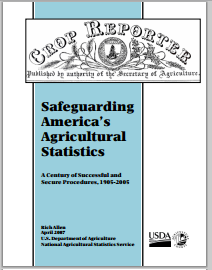
\includegraphics{images/NASS_History.png}

}

\caption{Figure 1: Safeguarding America's Agricultural Statistics: A
century of Successful and Secure Procedures}

\end{figure}%

Source:
\href{pdf-Readings/safegaurding-americas-agricultural-statistics.pdf}{NASS:
About Nass}

\begin{quote}
\section{Excerpt From Chapter 1}\label{excerpt-from-chapter-1-1}

The summary and release procedures for the USDA Bureau of Statistics'
reports in the early 1900s produced separate summary tabulations for
each data source available (up to six sources, in some cases)\ldots{} It
is also relevant that the release time for cotton reports in those years
was noon, Eastern Time, and that the commodity markets discontinued
trading for an hour starting at noon on release days. The original
procedures allowed the three people who had determined the final numbers
to go about their business, or even leave the building if they wished,
once a report's contents had been set.

In 1904 there were rumors about insider trading. As came to light later,
one of the three Bureau of Statistics people, E.S. Holmes, Jr., did have
an outside partner, a NewYork cotton trader named Louis Van Riper.
Shortly after an estimate was set, Holmes would meet Van Riper and tell
him what cotton estimate was going to be published. Van Riper would take
whatever market action would be most profitable based on the advance
information.

The scheme came to light following the cotton acreage report issued on
June 2, 1905. The three members met and adopted the state and national
figures to be published. After Holmes had sent his signal, one of the
other people who had worked on the report asked for reconsideration.
After further review, the figures to be published were revised. At that
point, the outside partner had already interpreted the original signal
and proceeded to place trades. The scheme came to light when Van Riper
charged in a telegram that a ``fraudulent'' report had been released. In
explaining why he thought this was a false report, he unwittingly
revealed that he had the information ahead of time. Evidently, Holmes'
outside partner had an overabundance of ego, but not a good balance of
common sense in going public with his story. (Allen 2007)
\end{quote}

This story is quite similar to the plot line of the 1980's movie,
\href{http://www.imdb.com/title/tt0086465/}{Trading Places}.\footnote{Anyone
  interested in a career in trading should watch this movie and then
  watch it again. You still hear references to the movie.} Where the
protagonists (Dan Aykroyd and Eddie Murphey) trick to antagonists, the
Duke Brothers by replacing the `Orange Juice Crop Report' that they
obtained illegally with a forged one that would cause exactly the
opposite price effect. They started buying before the report to profit
and Dan Aykroyd and Eddie Murphey start selling based on the correct
crop report information. The frenzy on the trading floor captures the
feeling of what happens during crop reports that move the market, even
if there is no longer trading on a physical floor as shown in the movie.

\section{Changing Report Release
Times}\label{changing-report-release-times-1}

Timing of report releases has important implications for the market
reaction as well. Figure 2 below provides a brief history of report
release times of major market sensitive reports.

\begin{figure}[H]

{\centering 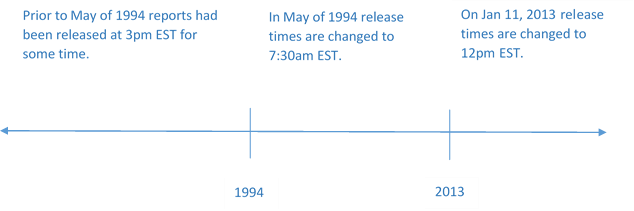
\includegraphics{images/NASS_release_timeline.png}

}

\caption{Figure 2: Timeline of Report Release Times}

\end{figure}%

Prior to 1994 most market sensitive USDA reports were released at 3pm
EST. This made sense from the USDA workflow perspective because it
allowed the lock-down to be enacted during normal working hours,
minimizing disruption of the analysts' regular lives. By the early 90's
releasing the report at this time became unpopular with market
participants. By releasing the report late in the afternoon in the U.S.
futures markets in other parts of the world could trade the USDA numbers
overnight before the U.S. market had a chance to react. Therefore price
discovery after reports was essentially shifted from Chicago to other
major exchanges across the world.

In May of 1994, the USDA shifted the release time to 8:30am EST. This
meant the report was released during regular business hours in the U.S.
and just one hour before trading begins on the U.S. futures exchange.
While clearly preferable to market participants in the U.S. this moved
the USDA's lockup time to overnight hours (Allen 2007).

By 2011, presumably due to the ability to trade electronically with high
speed, there was a desire for the futures market to be open and actively
trading at the time USDA reports were released. In this case, the
futures exchange acted first, expanding trading hours to an earlier
market open. Eventually, since futures market participants wanted it,
and because came with the added benefit of moving the beginning of the
lockup period from late night to early morning, the USDA began releasing
most reports at 12pm EST on January 11, 2013.

\section{Price Reactions}\label{price-reactions-1}

Market prices react strongly to USDA reports when the reports inject
significant and unanticipated information into the market. Some reports
are more likely than others to produce fireworks in terms of market
price.

\begin{longtable}[]{@{}
  >{\raggedright\arraybackslash}p{(\columnwidth - 4\tabcolsep) * \real{0.1509}}
  >{\raggedright\arraybackslash}p{(\columnwidth - 4\tabcolsep) * \real{0.0943}}
  >{\raggedright\arraybackslash}p{(\columnwidth - 4\tabcolsep) * \real{0.7484}}@{}}
\caption{Table 1: Reports most likely to cause significant movements in
market price}\tabularnewline
\toprule\noalign{}
\begin{minipage}[b]{\linewidth}\raggedright
Report
\end{minipage} & \begin{minipage}[b]{\linewidth}\raggedright
Dates
\end{minipage} & \begin{minipage}[b]{\linewidth}\raggedright
Reason
\end{minipage} \\
\midrule\noalign{}
\endfirsthead
\toprule\noalign{}
\begin{minipage}[b]{\linewidth}\raggedright
Report
\end{minipage} & \begin{minipage}[b]{\linewidth}\raggedright
Dates
\end{minipage} & \begin{minipage}[b]{\linewidth}\raggedright
Reason
\end{minipage} \\
\midrule\noalign{}
\endhead
\bottomrule\noalign{}
\endlastfoot
Grain Stocks & Quarterly & Information about scarcity or surplus of
supplies \\
Prospective Plantings & End of March & Acreage and therefore production
estimates \\
Planted Acres & End of June & Acreage and therefore production
estimates \\
WASDE & October & Some years the Oct report will contain significant
revisions from previous estimate \\
WASDE & January & Final production estimate for the preceding harvest.
Sometimes includes and unanticipated revision \\
Crop Progress Report & Weekly & Condition estimates. Only moves market
prices if significant deterioration associated with a drought or flood
occurs \\
\end{longtable}

\begin{description}
\item[Grain stocks]
Estimates only come out quarterly. Since the information about whether
we have a scarcity or surplus is a primary driver of price, and since we
only get this report four times per year, the stocks estimate can cause
significant adjustments in price.
\item[Prospective Planting and Planted Acres]
Reports give a baseline expectation about production for the coming
marketing year. Deviations from expectations or recent history will
cause rapid adjustments in price.
\item[WASDE]
The reports in October and January are relatively more likely to cause
rapid price adjustments than other months because in October the yield
estimates tend to become more precise and can involve significant
revisions from the previous month's estimate. Similarly, January report
contains finalized estimates of the crop production and in some cases
will involve unexpected revisions from previous estimates.
\item[Crop Progress]
These reports generally only move markets when crop conditions are
deteriorating rapidly due to drought or excess moisture. During years
with more typical weather, this report does not affect markets much
week-to-week.
\end{description}

\subsection{Some Examples of Recent Big Market
Reactions}\label{some-examples-of-recent-big-market-reactions-1}

Using the Best Bid Best Offer database from the CME Group's
\href{http://www.cmegroup.com/market-data/datamine-historical-data/}{DataMine}
we can examine historical intraday transaction prices (like what is
available streaming in real-time from Yahoo Finance or other sources).
These data are time-stamped to the second and allow the most accurate
and fine scale picture of futures market trading tick-by-tick.

Three examples come from the 2010 marketing year.

The June 30 Planted Acres report resulted in the market opening (at
8:30am EST) 15 cents higher than it closed the overnight trade just two
hours earlier. Ultimately it closed the day trading session 3.54
cents/bushel - 7.5\% or 25 cents higher than the most recent pre-report
price. Two put that into perspective, 25 cents that is an increase in
value of one futures contract of \$1,250, since future contracts are
specified for a quantity of 5,000 bushels.

Figure 2: Price of July 2010 corn on June 30, 2010 before and after the
release of Planted Acres Report

\includegraphics{12-ForecastingProduction_files/figure-pdf/unnamed-chunk-1-1.pdf}

In the top panel of Figure 2 you can see that the time stamps indicate
those are transactions occurring in the overnight electronic market.
There is a break in the morning prior to 9:30 CST when trading begins in
the daytime session. It is in this period that the Planted Acres report
is released. The bottom panel only displays the daytime session, so that
you can see the trading action more clearly. Between 9:30am and about
10:15 the market trades in a 10 cent range.

The Oct 8th WASDE report caused the market to open limit up. The
exchange sets the maximum fluctuation a futures price can trade in a
given day. The value of the limit can change at the discretion of the
exchange with some advance notice. The report indicated a sharp drop in
forecasted yield for corn. This resulted in the ending stocks number for
the 2010/2011 marketing year forecast below 1 billion bushels with a
very low stocks to use ratio as well. The market reaction is show below
in Figure 3.

Figure 3: Price of December 2010 corn on October 8th, 2010 before and
after the release of the WASDE Report

\includegraphics{12-ForecastingProduction_files/figure-pdf/unnamed-chunk-2-1.pdf}

The flat line during the daytime trading session is apparent, resulting
from prices being locked at the limit during the entire trading day.

Figure 5: Price of May 2011 corn on March 31st, 2011 before and after
the release of the Planted Acres Report

\includegraphics{12-ForecastingProduction_files/figure-pdf/unnamed-chunk-3-1.pdf}

This report indicated that corn acreage was to be higher than previously
expected, but corn stocks were lower than expected. The stocks number
dominated the price direction strongly and the market traded limit up on
this day as well.

\section{Conclusions}\label{conclusions-1}

This chapter reviewed the history of report released by the USDA. We
noted a data leak in 1905 led the agency to consider security from an
early date - a important component of report production that persists to
this day. We also learned that the Prospective Plantings, Planted
Acreage, October WASDE, January WASDE, and Grain Stocks reports are the
most likely to produce rapid price adjustments in the market. Some
specific examples were given, and depicted through charts of transaction
prices.

\bookmarksetup{startatroot}

\chapter{Forecasting Use of Corn}\label{forecasting-use-of-corn}

{Interested in more? Please let me know by}
\href{https://forms.gle/Q3VByCQZHjfQSy9D7}{taking the survey}!

In the WASDE balance sheet for corn there are three use categories. Two
account for domestic consumption - Food, Seed and Industrial, and Feed
and Residual - while exports make up the third category. Ethanol makes
up a large portion of the Food, Seed, and Industrial category, so it is
given its own line in the balance sheet.

As we have noted before, historical use patterns are the first place to
start when trying to forecast use categories for the marketing year.
Looking at quarterly gives you a sense of how use is distributed across
the marketing year in different categories. The annual histories,
however, are probably the most useful.

\includegraphics{assets/ForecastingUseof-CornUseCategories.png}

\section{Food, Alcohol, and Industrial
Use}\label{food-alcohol-and-industrial-use}

Let us begin by looking at the Food, Alcohol and Industrial category.
These data were queried from the
\href{http://www.ers.usda.gov/data-products/feed-grains-database/feed-grains-yearbook-tables.aspx\#26780}{Feed
Grains database} maintained by the USDA ERS. The categories here are a
little more disaggregated than those presented in the USDA WASDE balance
sheets, but they are roughly the same. For example, in figure 1 below we
show the \emph{Food, Alcohol, and Industrial} use category. This omits
seed from the \emph{Food, Seed, and Industrial} category in the WASDE
balance sheet. The Feed Grains database actually breaks out the seed use
as its own column, but corn used for seed is a very small proportion of
production and it is largely predictable from year to year.

\includegraphics{assets/ForecastingUseof-CornUseCategoriesFoodAlcoholInd.png}
Source:
\href{http://www.ers.usda.gov/data-products/feed-grains-database/feed-grains-yearbook-tables.aspx\#26780}{Feed
Grains database} maintained by the USDA ERS.

Figure 1 shows a dramatic uptrend in the Food, Alcohol and Industrial
use category. This is due to the dramatic increase in the production of
ethanol starting around 2005/2006 and plateauing around 2010 when U.S.
ethanol consumption roughly hit the `blend-wall' where ethanol makes up
10\% of the retail gasoline supply.

\includegraphics{assets/ForecastingUseof-CornUseCategoriesFoodAlcoholIndMY.png}
Source:
\href{http://www.ers.usda.gov/data-products/feed-grains-database/feed-grains-yearbook-tables.aspx\#26780}{Feed
Grains database} maintained by the USDA ERS.

Figure 2 shows the same data, but the quarterly figures are aggregated
to the marketing year total. In both figures 1 and 2 the rationing
effects of high prices that occurred as a result of the drought in 2012.

\includegraphics{assets/ForecastingUseof-CornUseCategoriesFoodAlcoholIndPropofUse.png}
Source:
\href{http://www.ers.usda.gov/data-products/feed-grains-database/feed-grains-yearbook-tables.aspx\#26780}{Feed
Grains database} maintained by the USDA ERS.

From figure 3 it is easier to see what share of the crop the large
increase in corn use in the Food, Alcohol, and Industrial use category.
In figure 3 this use category is presented as a percentage of that
marketing year's production. In the early 1990's this use category
accounted for over 50\% since 2010. The drop in percentage of production
in 2015 occurs because of the large crop in 2015, even though the use
level is flat (shown in figure 2).

\section{Exports}\label{exports}

Quarterly corn exports are displayed in figure 4. Unlike Food, alcohol
and industrial use, exports tend to have a very seasonal or cyclical
pattern. Exports are large in the second quarter of the marketing year,
December to February, right after we harvest the new crop. This is when
stocks are most plentiful and prices are at season lows in years
exhibiting an upward sloped forward curve.

\includegraphics{assets/ForecastingUseof-CornUseCategoriesExports.png}

Source:
\href{http://www.ers.usda.gov/data-products/feed-grains-database/feed-grains-yearbook-tables.aspx\#26780}{Feed
Grains database} maintained by the USDA ERS.

Displaying the same data in Figure 5, but aggregating to an annual
frequency, we see the marketing seasonality smoothed away.

\includegraphics{assets/ForecastingUseof-ExportsMY.png}

Source:
\href{http://www.ers.usda.gov/data-products/feed-grains-database/feed-grains-yearbook-tables.aspx\#26780}{Feed
Grains database} maintained by the USDA ERS.

On average, it appears that exports follow a constant trend-line with
variation around the mean produced by years of surplus or scarcity. The
drought year 2012, for example is clearly visible as an exceedingly low
export year.

In figure 6 we display annual corn exports as a percentage of corn
production.

\includegraphics{assets/ForecastingUseof-CornUseCategoriesExportsPropofUse.png}
Source:
\href{http://www.ers.usda.gov/data-products/feed-grains-database/feed-grains-yearbook-tables.aspx\#26780}{Feed
Grains database} maintained by the USDA ERS.

When exports are viewed as a proportion of production, we see a
pronounced downward trend. This is due to the increasing share of
production allocated to the Food, seed, and Industrial category visible
in figure 3. Recall that this category is comprised mainly of corn as
feed-stock for ethanol production.

The year-to-year variation is caused by price fluctuations with low
prices encouraging and high prices discouraging consumption. The
marketing year 2020 has shown a dramatic uptick in expected exports both
in millions of bushels and as a proportion of total use. A dramatic
increase in buying from China relative to previou levels has been the
biggest contributor.

: Table 1: Top 12 Importers of U.S. Corn 2012/2013 through 2016/2017
Marketing Years, Ranked in Descending Order for Marketing Year 2015/2016
(1,000 Metric Tons)

\begin{longtable}[]{@{}
  >{\raggedright\arraybackslash}p{(\columnwidth - 16\tabcolsep) * \real{0.0800}}
  >{\raggedright\arraybackslash}p{(\columnwidth - 16\tabcolsep) * \real{0.1800}}
  >{\raggedright\arraybackslash}p{(\columnwidth - 16\tabcolsep) * \real{0.0500}}
  >{\raggedright\arraybackslash}p{(\columnwidth - 16\tabcolsep) * \real{0.1800}}
  >{\raggedright\arraybackslash}p{(\columnwidth - 16\tabcolsep) * \real{0.0500}}
  >{\raggedright\arraybackslash}p{(\columnwidth - 16\tabcolsep) * \real{0.1800}}
  >{\raggedright\arraybackslash}p{(\columnwidth - 16\tabcolsep) * \real{0.0500}}
  >{\raggedright\arraybackslash}p{(\columnwidth - 16\tabcolsep) * \real{0.1800}}
  >{\raggedright\arraybackslash}p{(\columnwidth - 16\tabcolsep) * \real{0.0500}}@{}}
\toprule\noalign{}
\begin{minipage}[b]{\linewidth}\raggedright
COUNTRY
\end{minipage} & \begin{minipage}[b]{\linewidth}\raggedright
EXPORTS 2016/2017
\end{minipage} & \begin{minipage}[b]{\linewidth}\raggedright
RANK
\end{minipage} & \begin{minipage}[b]{\linewidth}\raggedright
EXPORTS 2015/2016
\end{minipage} & \begin{minipage}[b]{\linewidth}\raggedright
RANK
\end{minipage} & \begin{minipage}[b]{\linewidth}\raggedright
EXPORTS 2014/2015
\end{minipage} & \begin{minipage}[b]{\linewidth}\raggedright
RANK
\end{minipage} & \begin{minipage}[b]{\linewidth}\raggedright
EXPORTS 2013/2014
\end{minipage} & \begin{minipage}[b]{\linewidth}\raggedright
RANK
\end{minipage} \\
\midrule\noalign{}
\endhead
\bottomrule\noalign{}
\endlastfoot
MEXICO & 13539.7 & 1 & 12558.6 & 1 & 10793.8 & 2 & 10526.3 & 2 \\
JAPAN & 11983.4 & 2 & 10506.6 & 2 & 11858.6 & 1 & 11487.0 & 1 \\
KOR REP & 5588.5 & 3 & 3021.6 & 4 & 3927.2 & 4 & 4844.2 & 3 \\
COLOMB & 4438.9 & 4 & 4629.5 & 3 & 4413.3 & 3 & 3359.4 & 4 \\
PERU & 3166.7 & 5 & 2490.9 & 5 & 2421.0 & 5 & 1414.5 & 8 \\
TAIWAN & 2773.2 & 6 & 2045.2 & 6 & 1755.0 & 6 & 1936.4 & 7 \\
S ARAB & 2240.4 & 7 & 1516.4 & 7 & 1312.7 & 8 & 1021.0 & 9 \\
GUATMAL & 1008.9 & 8 & 897.1 & 10 & 936.7 & 9 & 783.9 & 11 \\
MOROCCO & 905.3 & 9 & 438.4 & 15 & 310.9 & 18 & 201.2 & 22 \\
C RICA & 840.2 & 10 & 520.1 & 13 & 784.1 & 11 & 593.6 & 13 \\
DOM REP & 814.9 & 11 & 252.1 & 22 & 599.3 & 13 & 637.6 & 12 \\
CHINA & 717.9 & 12 & 184.8 & 24 & 473.5 & 15 & 2759.4 & 5 \\
\end{longtable}

Source: \href{http://apps.fas.usda.gov/export-sales/myrk_rpt.htm}{USDA
FAS}

Table 1 shows the top 12 importers of U.S. corn for the 2016/2017
marketing year. Export totals are given in 1,000 metric ton units.
Clearly Japan and Mexico are the dominant Importers of U.S. corn, with
South Korea being a distant third. The table shows that most countries
rank has remained fairly stable across the marketing years shown.

\section{Feed and Residual}\label{feed-and-residual}

The final use category is the most difficult to forecast because its
quantity is derived, not estimated. This means the USDA makes estimates
of every other row in the balance sheet. Then, to ensure the numbers add
up, they infer the Feed and Residual category by subtracting the other
demand categories from supply.

\(Feed\&Residual = Production + Imports + Beginning Stocks - Ending Stocks - FoodSeed\&Industrial - Exports\)

Since each category on the right hand side is itself estimated with some
error, the error for the Feed and Residual category is the sum of the
errors of the other categories. This means that forecast errors from
each of the categories get added together, creating a category with
larger forecast error than all the others. For this reason the Feed and
Residual category is the most difficult to forecast. It should correlate
roughly to livestock feeding units, but does not prove to be that
effective in practice.

\(\begin{align} Feed\&Residual = (Production + \epsilon_{prod}) + (Imports + \epsilon_{import}) + (Beginning Stocks + \epsilon_{BStocks}) \\ - (Ending Stocks + \epsilon_{EStocks}) - (FoodSeed\&Industrial + \epsilon_{Food}) - (Exports + \epsilon_{Export}) \end{align}\)

Figure 7 below displays the Feed and Residual category since 1990.

\includegraphics{assets/ForecastingUseof-CornUseCategoriesFeedResid.png}

Source:
\href{http://www.ers.usda.gov/data-products/feed-grains-database/feed-grains-yearbook-tables.aspx\#26780}{Feed
Grains database} maintained by the USDA ERS.

Unlike Exports which saw its biggest quarter of use in the second
quarter of the marketing year (beginning in December), the biggest
quarter of use in the Feed and Residual category is the first (beginning
in September). This is because at the end of summer ranchers `bring
cattle home from grass' and they begin eating grain and hay instead of
green grass on pasture. This is also when calves born in the spring
begin to be `fattened' for slaughter.

Figure 8: shows the Feed and Residual category annually and figure 9
shows the category annually as a percent of production.

\includegraphics{assets/ForecastingUseof-FeedandResidualMY.png}

Source:
\href{http://www.ers.usda.gov/data-products/feed-grains-database/feed-grains-yearbook-tables.aspx\#26780}{Feed
Grains database} maintained by the USDA ERS.

\includegraphics{assets/ForecastingUseof-CornUseCategoriesFeedandResidPropofUse.png}

Source:
\href{http://www.ers.usda.gov/data-products/feed-grains-database/feed-grains-yearbook-tables.aspx\#26780}{Feed
Grains database} maintained by the USDA ERS.

Figure 8 shows that the category has remained roughly constant over the
time-period graphed, but as a percentage of production it has fallen
since 2005. Like the export category, this reflects a proportional shift
in use toward ethanol production.

\section{Price Sensitivity of Use
Categories}\label{price-sensitivity-of-use-categories}

Examining annual figures as a percentage of production reveals some
interesting facts about the price sensitivity of the three use
categories.

The least price sensitive category seems to be Food, Seed, and
Industrial. This should be intuitive because this category is composed
primarily of corn for feedstock in ethanol production. Since ethanol
consumption is effectively mandated at a certain level by the Renewable
Fuels Standard, users (gasoline blenders) must purchase a certain amount
of ethanol to blend into the retail gasoline supply. This implies a
significant portion of the corn crop that will be used regardless of the
price.

The second category is Feed and Residual. Although year-to-year
variation can come about due to price responsiveness of the U.S.
livestock industry, this variation tends to be overwhelmed by the
variation due to the aggregate forecast errors in the other categories.

The most price sensitive category is Exports, which is readily visible
in figure 5 and 6. Foreign buyers of corn can substitute to purchase
their corn from other parts of the world like (Argentina comes first to
mind). Also, consumers of meat (exported corn is primarily used as
animal feed in the foreign country) in the less developed world are more
price sensitive and presumably reduce consumption when prices are high.

\section{Forecasting Use}\label{forecasting-use}

One method for forecasting the use categories during the marketing year,
is to keep track of how much corn has been used to date in each
category. This pace of use can be compared to the pace of use in
previous years. Alternatively, the pace of use can be expressed as a
percent of the WASDE forecast use. Ideally this percent of WASDE
forecast use would be compared to historical percent of WASDE forecast
use. The idea behind such an exercise being the seasonality we saw in
the historical graphs above is likely to repeat itself. Information
about the pace of use in each category must be obtained from different
sources within the USDA.

\subsection{Food, Seed, and Industrial}\label{food-seed-and-industrial}

We discussed above that ethanol production is the primary user of corn
in the Food, Seed, and Industrial Category. This becomes obvious by
comparing figure 10 below, which displays ethanol production and
consumption over time, with figure 1 above.

\includegraphics{assets/ForecastingUseof-Ethanol.png}

Source:
\href{http://www.eia.gov/totalenergy/data/monthly/\#renewable}{EIA}
website. Click the link for access to the raw data.

Ethanol production and consumption begin to increase rapidly around
2005, which is when the Energy Policy Act of 2005 and later the Energy
Security and Independence Act of 2007 created the Renewable Fuels
Standard (RFS). The RFS mandated quantities of ethanol that blenders of
gasoline are required to blend into the retail gasoline supply. These
annual mandates are revised every year, but they were designed to
steadily increase year after year until 2015 when the mandate reached 15
billion gallons per year. This figure came about because gasoline
consumption in the United States was forecast to reach 150 billion
gallons per year by 2015. So the RFS mandates were designed to reach the
point where the entire retail gasoline supply would include 10\%
ethanol. Incidentally, 300,000,000 barrels indicated in Figure 10
corresponds to 15 billion gallons (300,000,000*50gallons/barrel =
15,000,000,000 gallons). The orange line shows that blenders of gasoline
have been blending greater than 15 billion gallons of ethanol since
2010.

Going forward, without significant growth in the consumption of gasoline
in the United States, this corn use category is likely to remain flat
for the foreseeable future. Even so, ethanol blenders sometimes
experience an ethanol-to-gasoline price ratio that is favorable to
blending ethanol even above the levels of the RFS mandate. So conducting
a pace-of-use analysis for this corn use category makes sense as well.
Data on monthly fuel ethanol production can be found at
\href{http://www.eia.gov/totalenergy/data/monthly/\#renewable}{EIA.GOV}.
Examining the current marketing year's production of ethanol gives some
indication of whether ethanol production is likely to exceed the 15
billion gallon per year mandated level.

\subsection{Exports}\label{exports-1}

Two USDA agencies are involved in providing estimates of export sales.
The \href{http://www.fas.usda.gov/}{USDA Foreign Agricultural Service}
and the \href{http://www.gipsa.usda.gov/}{USDA Grain Inspection,
Packers, and Stockyards Administration}.

\subsubsection{USDA FAS Export Sales Reporting
System}\label{usda-fas-export-sales-reporting-system}

The \href{http://www.fas.usda.gov/}{USDA Foreign Agricultural Service}
maintains the Export Sales Reporting System, which reports weekly export
quantities and daily reports of large export sales. From the FAS
\href{https://apps.fas.usda.gov/export-sales/FACT\%20SHEET.pdf}{website}:

\begin{quote}
The Export Sales Reporting Program has its roots from the unexpected
purchase of large amounts of grain by the Soviet Union in 1972, ``The
Great Russian Grain Robbery''. The huge, unanticipated purchases of U.S.
wheat and corn that year depleted U.S. reserve stocks which caused a
sizable run-up in U.S. food prices.

Furthermore, there was growing concern that some companies might have an
unfair advantage in situations like this because they had access to
market-sensitive information that was unavailable to the public. To
ensure that all parties involved in the production and export of U.S.
grain had access to up-to-date export information, Congress mandated the
Export Sales Reporting program in 1973.

Before the program was established, it was difficult for the public to
obtain information on exports until the products were actually shipped.
The program helps facilitate price stability by guaranteeing that
everyone has access to the same information at the same time.
\end{quote}

\subsection{Daily Reports}\label{daily-reports}

Under the export sales reporting system, U.S. exporters are required to
report all large sales of certain designated commodities by 3 p.m.
(Eastern time) on the next business day after the sale is made. The
designated commodities for these daily reports are wheat (by class),
barley, corn, grain sorghum, oats, soybeans, soybean cake and meal, and
soybean oil. Large sales for all reportable commodities except soybean
oil are defined as 100,000 metric tons or more of one commodity in one
day to a single destination or 200,000 tons or more of one commodity
during the weekly reporting period. Large sales for soybean oil are
20,000 tons and 40,000 tons, respectively. \textgreater{} \#\#\# Weekly
Reports Weekly reports are also required, regardless of the size of the
sales transaction, for all of these commodities, as well as wheat
products, rye, flaxseed, linseed oil, cotton (by staple length),
cottonseed, cottonseed cake and meal, cottonseed oil, rice (by class),
and cattle hides and skins (cattle, calf, and kip), and beef. The
reporting week for the export sales reporting system is Friday-Thursday.
The Secretary of Agriculture has the authority to add other commodities
to this list. Source:
\href{http://apps.fas.usda.gov/export-sales/backgrnd.htm\#Daily\%20Reports}{USDA
FAS}

\subsubsection{GIPSA}\label{gipsa}

USDA GIPSA mission is ``To facilitate the marketing of livestock,
poultry, meat, cereals, oil-seeds, and related agricultural products,
and promote fair and competitive trading practices for the overall
benefit of consumers and American agriculture.'' From the GIPSA website:

\begin{quote}
\subsection{History}\label{history}

The Grain Inspection, Packers and Stockyards Administration (GIPSA) was
established in 1994 as part of the reorganization of the U.S. Department
of Agriculture. The formation of the agency resulted from the joining of
two previously independent agencies: the Federal Grain Inspection
Service and the Packers and Stockyards Administration. Today, GIPSA is
part of USDA's Marketing and Regulatory Programs, which are working to
ensure a productive and competitive global marketplace for U.S.
agricultural products.

The Federal Grain Inspection Service (FGIS) was established by Congress
in 1976 to manage the national grain inspection system, which initially
was established in 1916, and to institute a national grain weighing
program. The goal of creating a single Federal grain inspection entity
was to ensure development and maintenance of uniform U.S. standards, to
develop inspection and weighing procedures for grain in domestic and
export trade, and to facilitate grain marketing.

Today's Packers and Stockyards Program (P\&S) is the progeny of the
Packers and Stockyards Administration, which was established in 1921
under the Packers and Stockyards Act. The organization was instituted to
regulate livestock marketing activities at public stockyards and the
operations of meat packers and live poultry dealers. Source:
\href{http://www.gipsa.usda.gov/about/mission.aspx}{USDA GIPSA}
\end{quote}

The GIPSA's main objective is to maintain standard in quality grading
and weighing, but as a by-product of their reporting they also produce
\href{http://www.gipsa.usda.gov/fgis/public_reports.aspx}{useful
statistics} on export shipments. Monthly data on grains inspected and
weighed for export by (U.S. region) and destination country is
available. Annual reports are also available.

Since the FAS and the GIPSA come about their export totals through
different processes, they will occasionally differ in their summary
estimates. They have a memorandum of understanding with one another that
differences will be reconciled so that the export totals reported by
each agency will not differ substantially.

\subsection{Feed and Residual}\label{feed-and-residual-1}

While the Residual component tends to dominate the variation in the Feed
and Residual category, the USDA does publish statistics related to
numbers of cattle, hogs, and poultry. Major changes in livestock numbers
produce a detectable impact in the Feed and Residual use category, to it
is worthwhile knowing where to find these estimates.

The USDA releases a monthly
\href{http://usda.mannlib.cornell.edu/MannUsda/viewDocumentInfo.do?documentID=1020}{Cattle
on Feed} report. Tracking this report gives a sense of trends in beef
cattle herd size and production. Similarly, the
\href{http://usda.mannlib.cornell.edu/MannUsda/viewDocumentInfo.do?documentID=1086}{Hogs
and Pigs} report is released quarterly and provides inventory estimates.
The monthly
\href{https://usda.mannlib.cornell.edu/MannUsda/viewDocumentInfo.do?documentID=1131}{Poultry
Slaughter} report contains the number of head and live weight of
chickens, turkeys, ducks and other poultry slaughtered under Federal
inspection.

\section{Readings}\label{readings-3}

\href{http://farmdocdaily.illinois.edu/2015/01/reviewing-pace-of-corn-and-soybean-exports.html}{Reviewing
the Pace of Corn and Soybean Exports}

Newton, J. ``Reviewing the Pace of Corn and Soybean Exports.'' farmdoc
daily (5):14, Department of Agricultural and Consumer Economics,
University of Illinois at Urbana-Champaign, January 26, 2015.

\bookmarksetup{startatroot}

\chapter{Forecasting Use of Soybeans}\label{forecasting-use-of-soybeans}

{Interested in more? Please let me know by}
\href{https://forms.gle/Q3VByCQZHjfQSy9D7}{taking the survey}!

In the WASDE balance sheet for soybeans there are three use categories.
Two account for domestic consumption - Crush, and Feed, Seed, and
Residual - while exports make up the third category. The main
distinction between cereal grains, like corn, and oilseeds, like
soybeans, is that cereal grains are generally ground whole for whatever
the end use turns out to be. Most oilseeds, on the other hand, are
crushed to extract oil and meal before their ultimate use. Soybean oil
is food-grade and can be found on the shelves of any American grocery
store. Soybean meal is protein rich and used as an ingredient in
livestock feed rations.

In the next sections we will examine historical use patterns of soybeans
in the three categories expressed nominally, and as a percent of the
concurrent year's total supply, similar to the organization of chapter
7.

Since this book has taken a closer look at corn production than soybean
production, we will ground our discussion of use by first noting the
pattern of annual supply of soybeans in recent history.

Figure 1 displays annual soybean production in millions of bushels from
1980-2014. A steadily increasing trend can be observed; supply had
roughly doubled since the early 1980s from about 2,300 million bushels
to about 4,000 million bushels in 2014.

\begin{figure}[H]

{\centering \includegraphics{Excel-files/ForecastingUseSoy-OilCropsYearbook_files/image013.png}

}

\caption{Figure 1: Annual Soybean Supply, 1980-2014}

\end{figure}%

Source:
\href{http://www.ers.usda.gov/data-products/oil-crops-yearbook.aspx}{USDA
ERS Oil Crops Yearbook}

Since soybeans are not consumed whole as food by humans or feed for
animals in the U.S., nearly all the soybean supply is crushed
domestically or exported.

\section{Soybean Crush}\label{soybean-crush}

Figure 2 displays the annual crush of soybeans from 1980-2014. A
pronounced upward trend, similar to the trend in soybean supply is
observed.

\begin{figure}[H]

{\centering \includegraphics{Excel-files/ForecastingUseSoy-OilCropsYearbook_files/image005.png}

}

\caption{Figure 2: Annual Soybean Crush, 1980-2014}

\end{figure}%

Source:
\href{http://www.ers.usda.gov/data-products/oil-crops-yearbook.aspx}{USDA
ERS Oil Crops Yearbook}

When examining corn use, we saw that the proportion of supply shifted
dramatically from other use categories to Food, Seed, and Industrial use
due to the increase in ethanol production since 2005. In figure 3, we
show soybean crush as a percent of the concurrent year's total supply.
While the bushels of soybeans devoted to the crush is steadily
increasing, figure 3 shows that the crush is increasing roughly
proportionally. There does not seem to be a shift into or out of the
crush category.

\begin{figure}[H]

{\centering \includegraphics{Excel-files/ForecastingUseSoy-OilCropsYearbook_files/image007.png}

}

\caption{Figure 3: Annual Soybean Crush as a Percent of Supply,
1980-2014}

\end{figure}%

Source:
\href{http://www.ers.usda.gov/data-products/oil-crops-yearbook.aspx}{USDA
ERS Oil Crops Yearbook}

\section{Exports}\label{exports-2}

Figure 4 displays annual soybean exports. Similar to the crush category,
exports are observed to steadily increase over the period from
1980-2014.

\begin{figure}[H]

{\centering \includegraphics{Excel-files/ForecastingUseSoy-OilCropsYearbook_files/image001.png}

}

\caption{Figure 4: Annual Soybean Exports, 1980-2014}

\end{figure}%

Source:
\href{http://www.ers.usda.gov/data-products/oil-crops-yearbook.aspx}{USDA
ERS Oil Crops Yearbook}

Figure 5 shows soybean exports as a percent of total supply from
1980-2014. Similar to the crush category, the percentage of supply has
remained constant.

\begin{figure}[H]

{\centering \includegraphics{Excel-files/ForecastingUseSoy-OilCropsYearbook_files/image009.png}

}

\caption{Figure 2: Annual Soybean Exports as a Percent of Supply,
1980-2014}

\end{figure}%

\begin{description}
\item[Source:
\href{http://www.ers.usda.gov/data-products/oil-crops-yearbook.aspx}{USDA
ERS Oil Crops Yearbook}]
Table 1: Top 10 Importers of U.S. Soybeans 2012/2013 through 2016/2017
Marketing Years, Ranked in Descending Order for Marketing Year 2016/2017
(1,000 Metric Tons)
\end{description}

\begin{longtable}[]{@{}
  >{\raggedright\arraybackslash}p{(\columnwidth - 16\tabcolsep) * \real{0.0891}}
  >{\raggedright\arraybackslash}p{(\columnwidth - 16\tabcolsep) * \real{0.1782}}
  >{\raggedright\arraybackslash}p{(\columnwidth - 16\tabcolsep) * \real{0.0495}}
  >{\raggedright\arraybackslash}p{(\columnwidth - 16\tabcolsep) * \real{0.1782}}
  >{\raggedright\arraybackslash}p{(\columnwidth - 16\tabcolsep) * \real{0.0495}}
  >{\raggedright\arraybackslash}p{(\columnwidth - 16\tabcolsep) * \real{0.1782}}
  >{\raggedright\arraybackslash}p{(\columnwidth - 16\tabcolsep) * \real{0.0495}}
  >{\raggedright\arraybackslash}p{(\columnwidth - 16\tabcolsep) * \real{0.1782}}
  >{\raggedright\arraybackslash}p{(\columnwidth - 16\tabcolsep) * \real{0.0495}}@{}}
\toprule\noalign{}
\begin{minipage}[b]{\linewidth}\raggedright
COUNTRY
\end{minipage} & \begin{minipage}[b]{\linewidth}\raggedright
EXPORTS 2016/2017
\end{minipage} & \begin{minipage}[b]{\linewidth}\raggedright
RANK
\end{minipage} & \begin{minipage}[b]{\linewidth}\raggedright
EXPORTS 2015/2016
\end{minipage} & \begin{minipage}[b]{\linewidth}\raggedright
RANK
\end{minipage} & \begin{minipage}[b]{\linewidth}\raggedright
EXPORTS 2014/2015
\end{minipage} & \begin{minipage}[b]{\linewidth}\raggedright
RANK
\end{minipage} & \begin{minipage}[b]{\linewidth}\raggedright
EXPORTS 2013/2014
\end{minipage} & \begin{minipage}[b]{\linewidth}\raggedright
RANK
\end{minipage} \\
\midrule\noalign{}
\endhead
\bottomrule\noalign{}
\endlastfoot
CHINA & 36148.3 & 1 & 29855.0 & 1 & 29640.8 & 1 & 27602.2 & 1 \\
MEXICO & 3665.0 & 2 & 3252.6 & 2 & 3438.8 & 2 & 3194.5 & 2 \\
INDNSIA & 2296.9 & 3 & 2028.6 & 5 & 1875.9 & 5 & 2291.5 & 3 \\
JAPAN & 2137.2 & 4 & 2145.6 & 3 & 2011.4 & 3 & 1826.4 & 4 \\
NETHLDS & 2044.9 & 5 & 2037.7 & 4 & 1879.4 & 4 & 1015.6 & 7 \\
TAIWAN & 1292.7 & 6 & 1232.9 & 7 & 1310.8 & 6 & 1133.6 & 5 \\
GERMANY & 1287.7 & 7 & 1757.5 & 6 & 1005.9 & 7 & 676.1 & 8 \\
BANGLADH & 1050.0 & 8 & 551.0 & 10 & 545.7 & 13 & 160.5 & 21 \\
THAILND & 950.6 & 9 & 424.2 & 15 & 518.2 & 14 & 432.4 & 13 \\
EGYPT & 807.2 & 10 & 295.4 & 19 & 712.4 & 11 & 604.6 & 9 \\
SPAIN & 731.8 & 11 & 964.1 & 8 & 852.4 & 8 & 1099.5 & 6 \\
KOR REP & 653.4 & 12 & 480.3 & 13 & 548.1 & 12 & 599.2 & 10 \\
\end{longtable}

Source: \href{http://apps.fas.usda.gov/export-sales/myrk_rpt.htm}{USDA
FAS}

Clearly China is the dominant importer of U.S. soybeans. They buy 10
times more than 2nd ranked Mexico. Examining the short history in table
1, you can see that increasing exports of soybeans to China accounts for
nearly all of the uptrend in figure 4. In the 2016/2017 marketing year
China was the destination of over 60\% of U.S. soybean exports.

\section{Feed, Seed, and Residual}\label{feed-seed-and-residual}

\begin{figure}[H]

{\centering \includegraphics{Excel-files/ForecastingUseSoy-OilCropsYearbook_files/image003.png}

}

\caption{Figure 6: Annual Soybean Feed, Seed, and Residual, 1980-2014}

\end{figure}%

Source:
\href{http://www.ers.usda.gov/data-products/oil-crops-yearbook.aspx}{USDA
ERS Oil Crops Yearbook}

\begin{figure}[H]

{\centering \includegraphics{Excel-files/ForecastingUseSoy-OilCropsYearbook_files/image012.png}

}

\caption{Figure 7: Annual Soybean Feed, Seed, and Residual as a Percent
of Supply, 1980-2014}

\end{figure}%

Source:
\href{http://www.ers.usda.gov/data-products/oil-crops-yearbook.aspx}{USDA
ERS Oil Crops Yearbook}

\section{Price Sensitivity of Use
Categories}\label{price-sensitivity-of-use-categories-1}

Soybeans are a bit different from corn because there are only two use
categories that are important, crush and exports. The soybean use
categories historically have been reliably 50\% crush and 50\% exports
as a percent of supply. In recent years, exports have been increasing
both nominally and as a percent of supply. So forecasting demand for
soybeans has largely become a matter of forecasting soybean exports.

Recently, with the rise of South American soybean (and corn) production,
forecasting exports is a matter of balancing the price of U.S soybeans
compared with the price of South American soybeans and the raw demand
from our trading partners. China has become the major player in this
space, as is evident in table 1.

\section{Forecasting Use of
Soybeans}\label{forecasting-use-of-soybeans-1}

As we mentioned in chapter 7, keeping track of how much soybeans have
been used to date in each category is a useful exercise to determine a
reasonable forecast for different use categories of soybeans. As was
true for corn, information about the pace of use in each category must
be obtained from different sources within the USDA.

Soybeans exports can be followed during the marketing year by following
the \href{}{GIPSA} and \href{}{FAS Export Reporting System} as was
identified for corn exports in Chapter 7. Also, as identified in Chapter
7 is is useful to tracking
\href{http://usda.mannlib.cornell.edu/MannUsda/viewDocumentInfo.do?documentID=1020}{Cattle
on Feed},
\href{http://usda.mannlib.cornell.edu/MannUsda/viewDocumentInfo.do?documentID=1086}{Hogs
and Pigs}, and the
\href{https://usda.mannlib.cornell.edu/MannUsda/viewDocumentInfo.do?documentID=1131}{Poultry
Slaughter}, specifically because livestock numbers contribute to demand
for soybean meal, which in turn contributes to crush demand.

\section{Exercises}\label{exercises-3}

\textbf{Skills Learned}

\begin{itemize}
\item
  A common method for accounting strength of demand: pace of use.
\item
  How to directly import data that is hosted on a website so that a .csv
  file has a url for download
\item
  How to work with pivot tables in excel to summarize large data-sets
  with many factor variables
\end{itemize}

Compare the pace of export sales in the first few weeks of marketing
year 2017/2018 to the pace of export sales in the previous three
marketing years. Make inferences about whether this marketing year seems
to be getting off to a good start in export sales.

\begin{enumerate}
\def\labelenumi{\arabic{enumi}.}
\tightlist
\item
  Go to \url{https://www.gipsa.usda.gov/}
\end{enumerate}

\begin{verbatim}
a. Choose FGIS Reports in the Federal Grain Inspection Menu  

b. Scroll down and choose Export Grain Totals (Yearly) in the Data and Statistics section  
\end{verbatim}

\begin{enumerate}
\def\labelenumi{\arabic{enumi}.}
\setcounter{enumi}{1}
\tightlist
\item
  Import the reports for 2014-2017 into excel so we can examine the
  following marketing years:
\end{enumerate}

\begin{verbatim}
a. 2014/2015, 2015/2016, 2016/2017, and 2017/2018 (so far)  
\end{verbatim}

\begin{enumerate}
\def\labelenumi{\arabic{enumi}.}
\setcounter{enumi}{2}
\item
  Create a pivot table that has weeks in the rows, marketing year in the
  columns, and sums the export sales in each week. Filter by Grain.
\item
  Copy and paste special this table into a new worksheet as plain text
  (so that is not a pivot table).
\item
  Delete the data in 2014 prior to September so that we start at the
  beginning of the marketing year.
\item
  Collapse all the marketing year into a single set of 53 rows (so we
  can compare by marketing year.)
\item
  Create a new column on the left side and fill it in with a sequence of
  1 to 53, for weeks in the marketing year.
\item
  Insert two columns between each marketing year; label them Cumulative
  Sum and Pace of Export.
\item
  Calculate the cumulative sums.
\item
  Go find the historical export numbers from old WASDE reports for each
  marketing year. Enter these values in your spreadsheet somewhere, and
  convert the million bushel numbers into pounds using the fact that
  bushel of soybeans weighs about 60 lbs.
\item
  Calculate the pace of use by dividing the cumulative sums by the
  export total for each marketing year.
\item
  Plot the pace of use with the Week numbers on the x axis for each
  marketing year.
\item
  Infer whether or not the 2017/2018 export sales are off to a strong
  start.
\end{enumerate}

\bookmarksetup{startatroot}

\chapter{Ending Stocks and Price}\label{ending-stocks-and-price}

{Interested in more? Please let me know by}
\href{https://forms.gle/Q3VByCQZHjfQSy9D7}{taking the survey}!

Over the course of the last several chapters we have covered each
category of supply and use. In tables 1 and 2 below, that literally
means we covered how to forecast the numbers in each row of the USDA
WASDE balance sheet. Subtracting total use from total supply gives an
estimate of marketing year ending stocks. For example, in table 1,

\[Supply, Total - Use, Total = 16,909 - 14,500 = 2,409 (Million bushels) = Ending Stocks;\]

in table 2{[}\^{}adding{]}

\[Supply, Total - Use, Total = 4,426 - 4,061 = 365 (Million bushels) = Ending Stocks\]

\begin{description}
\item[{[}\^{}adding{]}: Recall that WASDE balance sheets do not always
add perfectly due to rounding.]
Table 1. September 2016 USDA WASDE Balance Sheet for Corn
\end{description}

\begin{longtable}[]{@{}
  >{\raggedright\arraybackslash}p{(\columnwidth - 8\tabcolsep) * \real{0.1627}}
  >{\raggedright\arraybackslash}p{(\columnwidth - 8\tabcolsep) * \real{0.1506}}
  >{\raggedright\arraybackslash}p{(\columnwidth - 8\tabcolsep) * \real{0.1807}}
  >{\raggedright\arraybackslash}p{(\columnwidth - 8\tabcolsep) * \real{0.2470}}
  >{\raggedright\arraybackslash}p{(\columnwidth - 8\tabcolsep) * \real{0.2590}}@{}}
\toprule\noalign{}
\begin{minipage}[b]{\linewidth}\raggedright
Corn
\end{minipage} & \begin{minipage}[b]{\linewidth}\raggedright
Marketing Year 2014/2015
\end{minipage} & \begin{minipage}[b]{\linewidth}\raggedright
Marketing Year 2015/2016 Est.
\end{minipage} & \begin{minipage}[b]{\linewidth}\raggedright
Marketing Year 2016/2017 July Projection
\end{minipage} & \begin{minipage}[b]{\linewidth}\raggedright
Marketing Year 2016/2017 August Projection
\end{minipage} \\
\midrule\noalign{}
\endhead
\bottomrule\noalign{}
\endlastfoot
\textbf{Million Acres} & & & & \\
Area Planted & 90.6 & 88 & 94.1 * & 94.1 \\
Area Harvested & 83.1 & 80.7 & 86.6 * & 86.6 \\
\textbf{Bushels} & & & & \\
Yield per Harvested Acre & 171 & 168.4 & 168.0 * & 175.1 \\
\textbf{Million Bushels} & & & & \\
Beginning Stocks & 1232 & 1731 & 1701 & 1706 \\
Production & 14216 & 13601 & 14540 & 15153 \\
Imports & 32 & 65 & 40 & 50 \\
\textbf{Supply, Total} & \textbf{15479} & \textbf{15397} &
\textbf{16281} & \textbf{16909} \\
Feed and Residual & 5314 & 5200 & 5500 & 5675 \\
Food, Seed \& Industrial & 6567 & 6567 & 6650 & 6650 \\
\emph{Ethanol \& by-products} & \emph{5200} & \emph{5200} & \emph{5275}
& \emph{5275} \\
Domestic, Total & 11881 & 11767 & 12150 & 12325 \\
Exports & 1867 & 1925 & 2050 & 2175 \\
\textbf{Use, Total} & \textbf{13748} & \textbf{13692} & \textbf{14200} &
\textbf{14500} \\
Ending Stocks & 1731 & 1706 & 2081 & 2409 \\
\textbf{Avg. Farm Price (\$/bu)} & \textbf{3.7} & \textbf{3.55 - 3.65} &
\textbf{3.10 - 3.70} & \textbf{2.85 - 3.45} \\
\end{longtable}

\begin{description}
\item[and]
Table 2. September 2016 USDA WASDE Balance Sheet for Soybeans
\end{description}

\begin{longtable}[]{@{}
  >{\raggedright\arraybackslash}p{(\columnwidth - 8\tabcolsep) * \real{0.1627}}
  >{\raggedright\arraybackslash}p{(\columnwidth - 8\tabcolsep) * \real{0.1506}}
  >{\raggedright\arraybackslash}p{(\columnwidth - 8\tabcolsep) * \real{0.1807}}
  >{\raggedright\arraybackslash}p{(\columnwidth - 8\tabcolsep) * \real{0.2470}}
  >{\raggedright\arraybackslash}p{(\columnwidth - 8\tabcolsep) * \real{0.2590}}@{}}
\toprule\noalign{}
\begin{minipage}[b]{\linewidth}\raggedright
Soybeans
\end{minipage} & \begin{minipage}[b]{\linewidth}\raggedright
Marketing Year 2014/2015
\end{minipage} & \begin{minipage}[b]{\linewidth}\raggedright
Marketing Year 2015/2016 Est.
\end{minipage} & \begin{minipage}[b]{\linewidth}\raggedright
Marketing Year 2016/2017 July Projection
\end{minipage} & \begin{minipage}[b]{\linewidth}\raggedright
Marketing Year 2016/2017 August Projection
\end{minipage} \\
\midrule\noalign{}
\endhead
\bottomrule\noalign{}
\endlastfoot
\textbf{Million Acres} & & & & \\
Area Planted & 83.3 & 82.7 & 83.7* & 83.7 \\
Area Harvested & 82.6 & 81.8 & 83* & 83 \\
\textbf{Bushels} & & & & \\
Yield per Harvested Acre & 47.5 & 48 & 48.9* & 50.6 \\
\textbf{Million Bushels} & & & & \\
Beginning Stocks & 92 & 191 & 255 & 195 \\
Production & 3927 & 3929 & 4060 & 4201 \\
Imports & 33 & 25 & 30 & 30 \\
\textbf{Supply, Total} & \textbf{4052} & \textbf{4145} & \textbf{4346} &
\textbf{4426} \\
Crushings & 1873 & 1900 & 1940 & 1950 \\
Exports & 1842 & 1880 & 1950 & 1985 \\
Seed & 96 & 97 & 95 & 95 \\
Residual & 50 & 12 & 31 & 31 \\
\textbf{Use, Total} & \textbf{3862} & \textbf{3889} & \textbf{4016} &
\textbf{4061} \\
Ending Stocks & 191 & 255 & 330 & 365 \\
\textbf{Avg. Farm Price (\$/bu)} & \textbf{10.1} & \textbf{8.95} &
\textbf{8.35 - 9.85} & \textbf{8.30 - 9.80} \\
\end{longtable}

However, this still leaves a lot to be desired because the most
compelling reason to keep a detailed balance sheet and forecast future
supply and use is to come up with a reasonable expectation for price.
After all our work on forecasting the components of the balance sheet,
we have not made much headway in that regard. In this chapter, we cover
some approaches for taking a forecast of ending stocks and translating
that into a forecast of price.

\section{Forecasting Price}\label{forecasting-price}

Arriving at an estimate of ending stocks gives one a sense of the degree
of scarcity (or lack-thereof) in the market. It is still difficult to
infer the marketing year average price from that, because the prevailing
price that should coincide with the forecasted ending stocks is a
function of the elasticities of demand for different use categories.
These can be difficult to estimate, and we are not guaranteed that
elasticity is constant from one year to the next.

Figure 1 below is reproduced from the farmDoc Daily (fdd) article by
Good and Irwin, ``The Relationship between Stocks-to-Use and Corn Prices
Revisited''

\begin{figure}[H]

{\centering \includegraphics{images/fdd04092015_fig1.jpg}

}

\caption{Classic `Identification Problem' of Regressing Prices on
Quantities}

\end{figure}%

Source:
\href{http://farmdocdaily.illinois.edu/2015/04/relationship-stock-to-use-and-corn-prices.html}{FarmDoc
Daily}

Since the supply curve shifts from year-to-year and the demand curve
shifts from year-to-year due to a myriad of factors, one cannot count on
estimating a single supply or demand curve from a series of price and
quantity pairs. However, once we have entered a marketing year; i.e., we
have harvested the domestic supply in the balance sheet, we can count of
total supply being quite inelastic. We can be confident of this because
imports are historically a very small part of domestic total supply for
corn, and after the domestic harvest, imports would be the only way to
shift the supply curve. Further, if one had some confidence that the
demand curve was more or less constant through time, a time-series of
prices and quantities would approximately trace out the demand curve.

\section{Examining the Data}\label{examining-the-data}

This section continues to draw heavily on the Good and Irwin fdd article
referenced above. First let us take a look at the average price received
for corn over time and the stocks-to-use of corn over time in figure 2.
These data can both be obtained from the
\href{http://www.ers.usda.gov/data-products/feed-grains-database.aspx}{USDA
ERS Feed Grains Database} database, although you have to download the
\emph{stocks} and \emph{use} separately and create your own
stocks-use-variable.

\begin{figure}[H]

{\centering \includegraphics{assets/EndingStocksand-StocksUsePrices.png}

}

\caption{Figure 2: Corn Average Price Received and Stocks-to-Use}

\end{figure}%

Perhaps the first thing that one notices in this figure is the
pronounced stocks-to-use spikes that occurred in the 1982/1983 and
1985/1986, 1986/1987, 1987/1988 marketing years. Those exceptionally
high stocks relative to use was a result of government commodity
programs designed to keep prices from falling too far. Specifically, the
stocks were help primarily in the Farmer-Owned-Reserve or by the
Commodity Credit Corporation (Westcott and Hoffman 1999). Both programs
were designed to keep bushels off the market and thus buoying prices.
During periods of prolonged excesses, however, it becomes very costly
for the government to procure and store large quantities of the
commodity and it has a continuing depressing effect on market prices
because the market knows the government holds large stockpiles. Farm
legislation (`The Farm Bill' is re-negotiated every four years by
congress) has trended toward more market-oriented approaches to
supporting agriculture, and one can observe a marked decline in
stocks-to-use over time.

Aside from the the wild swings in the 1980's, the series still seem to
show a negative relationship between stocks-to-use and prices, as one
would expect. Figure 3 graphs these two series as a scatter-plot with
stocks-to-use on the x-axis.

\begin{figure}[H]

{\centering \includegraphics{assets/EndingStocksand-StocksUsePrices2.png}

}

\caption{Figure 3: Corn Prices vs.~Stocks-to-Use}

\end{figure}%

A clear negative relationship emerges, but the relationship when stocks
are less than 20\% of use is less clear. To help clarify, figure 4
highlights years before and after 2006.

\begin{figure}[H]

{\centering \includegraphics{assets/EndingStocksand-StocksUsePrices3.png}

}

\caption{Figure 4: Corn Prices vs Stocks-to-Use Pre- and Post-2006}

\end{figure}%

Highlighting the data and pre- or post-2006\footnote{The year 2006 here
  is assumed to be a transtion year and dropped from the figure. In
  2006, stock-to-use was 11.63\% and average price was \$3.04. Examining
  this data-point on Figure 4 suggests 2006 does not fit either regime
  well.} clearly shows a wide range of prices over a relatively narrow
range of stocks-to-use realizations. Given that 2006 is the beginning of
the ramp-up in ethanol production, this should not be surprising.
Suddenly there was a large and very inelastic demander of corn in the
market. This ensured supply would have to be rationed by price to keep
stocks from falling to low levels.

Also in figure 4 trendlines are fitted for the two subsets of the data.
Since both scatterplots appear to display a curvature, the price data
are regressed on the log of the stocks-to-use data. Also, this
specification provided the highest \(R^2\) of the regression
specifications available in the defalt Excel options. The regression in
the post-2006 period explains 80\% of the variaiton in the price data,
which suggests it is a reasonable starting point for forecasting price
using ending stocks and the balance sheet approach.

\section{References}\label{references}

Good, D., and S. Irwin.
``\href{http://farmdocdaily.illinois.edu/2015/04/relationship-stock-to-use-and-corn-prices.html}{The
Relationship between Stocks-to-Use and Corn Prices Revisited}.'' farmdoc
daily (5):65, Department of Agricultural and Consumer Economics,
University of Illinois at Urbana-Champaign, April 9, 2015.

\section{Exercises}\label{exercises-4}

\begin{enumerate}
\def\labelenumi{\arabic{enumi}.}
\item
  Go to \url{www.agmanager.info}, the extension website of Kansas State
  University's Agricultural Economics department.

  \begin{itemize}
  \item
    Navigate through the \emph{Grain Marketing} menu to the \emph{Grain
    Supply and Demand (WASDE)} page.
  \item
    Click on \emph{Spreadsheets with WASDE data}, or scroll to the
    bottom of the page.
  \item
    Download the \emph{Corn}, \emph{Soybeans}, and \emph{Wheat} WASDE
    tables.
  \item
    This data is also available from various USDA websites (like
    \url{https://quickstats.nass.usda.gov/}), but the
    \href{agmanager.info}{www.agmanager.info} site is particularly
    thorough and well organized for historical WASDE data, so it is a
    good resource to know about.
  \end{itemize}
\item
  Open all three Excel tables for corn, soybeans, and wheat.

  \begin{itemize}
  \item
    Also open a new Excel spreadsheet.
  \item
    For each of the commodities, corn, sobyeans, and wheat, go to the
    \emph{Annual Sheet}, then copy and paste the \emph{Year},
    \emph{Stock \%}, and \emph{Average Farm Price} columns into your new
    Excel Spreadsheet. Be sure to label the columns by commodity.
  \end{itemize}
\item
  For each commodity, Recreate figure 2 (a time-series chart of prices
  recieved by farmers and stocks/use \%) and figure 3 (an x-y
  scatterplot of prices recieved by farmers and stocks/use \%) from
  chapter 11.

  \begin{itemize}
  \item
    Fit an appropriate trendline through each of the x-y scatterplots.
  \item
    Make an educated forecast for average farm price recieved for each
    commodity.
  \end{itemize}
\end{enumerate}

\bookmarksetup{startatroot}

\chapter{The Soybean Crush}\label{the-soybean-crush}

{Interested in more? Please let me know by}
\href{https://forms.gle/Q3VByCQZHjfQSy9D7}{taking the survey}!

In this Chapter we describe the physical process of converting soybeans
into meal and oil, as well as the price relationship that is maintained
between these highly related commodities. We saw in the chapter,
`Forecasting Use of Soybeans in the WASDE Balance Sheet,' that
approximately half of the supply of soybeans in the U.S. is crushed into
soybean meal and oil. Nearly all of the remainder of soybean supply is
exported where most of it will be crushed abroad.

\includegraphics{images/soyoilmeal_checkoff.jpg} Source:
\href{http://unitedsoybean.org/}{United Soybean Board},
\href{https://www.flickr.com/photos/unitedsoybean/10059732523/in/photolist-gjWL1c-iSHsD6-gjRZN5-gjSiez-gjRDSm-3GTus-gjT5Pf-gjT5FQ-gjT5Zf-iRrGux-5mxrJp-iRuCDS-fEhEb4-iSHt56-gjSLAj-gjTptX-gjSLDL-gjSNeR-gjSLEC-gjT72q-6m2BCX-gjSUHT-gjTpzi-6m6Jay-qBtpPq-5wBq3U-gjWLbe-aMpXNc-qRDdLA-gjWY8m-rujuvk-iRqECD-rNDaeg-GL7Qd-6m2Yyc-6JGi4H-ar3khU-cNjfUf-6m2A3g-aE4dw4-c3VUt9-c3VVq5-4JzMWS-6KY45z-6m2Xsv-6m6Eny-6m2XZg-6m2WVa-6m2ZFF-6m7ad1}{Flicker}

\section{Oilseed Processing}\label{oilseed-processing}

Now the most prevalent method for crushing soybeans is a method that
uses a solvent to extract the oil from the soybean. Basically, soybeans
are pre-treated, then flaked to destroy the cell walls so the solvent
can get at the oil in the cells. A crude oil is then further processed
refined to remove the solvent and other compounds like glycerin, leaving
only pure soybean oil. The soybean flakes, minus the oil are then ground
in to meal that can be used as a high protein livestock feed.

\begin{figure}[H]

{\centering \includegraphics{images/soyflakes.jpg}

}

\caption{Soy Flakes}

\end{figure}%

Source: \href{http://unitedsoybean.org/}{United Soybean Board},
\href{https://www.flickr.com/photos/unitedsoybean/10059015936/}{Flicker}

\begin{figure}[H]

{\centering \includegraphics{images/soymeal.jpg}

}

\caption{Soymeal}

\end{figure}%

Source: \href{http://unitedsoybean.org/}{United Soybean Board},
\href{https://www.flickr.com/photos/unitedsoybean/10059074033/}{Flicker}

\begin{figure}[H]

{\centering \includegraphics{images/crush_products.jpg}

}

\caption{Intermediate Soy Oil Products}

\end{figure}%

Source: \href{http://unitedsoybean.org/}{United Soybean Board},
\href{https://www.flickr.com/photos/unitedsoybean/10058954054/}{Flicker}

Historically, soybeans were processed by feeding soybeans into a
mechanical press that literally squeezed the oil out. This process is
less efficient and more time consuming - thus more costly. Nearly all
commercially crushed soybeans are done with with the solvent extraction
method.

Crushing soybeans yields about 11lbs of oil and 44lbs meal per bushel of
soybeans, these yields can vary slightly, but most use these values in
the price analysis that will follow.

\section{Soybean Oil Uses}\label{soybean-oil-uses}

Soybean oil is used primarily as a food-grade product. It is not usually
found in grocery stores as 100\% soybean oil, but it will be present in
oil branded as `cooking oil' - where it is blended with other edible
oils like corn oil and canola (also known as rapeseed) oil. Composition
of cooking oil can vary from one purchase to the next as producers of
cooking oil can blend the edible oil components based on relative
prices.

Soybean oil also can be further processed into partially hydrogenated
soybean oil. This is accomplished by literally adding hydrogen to the
vegetable oil. The resulting product is widely used in processed food
such as baked goods, crackers, frozen foods; it is used in a lot of
processed foods generally speaking. It is a perfect ingredient in
processed foods because it is solid at room temperature, and essentially
never goes bad. If natural vegetable oils were used in processed foods
the oil would go rancid in a short period of time.

Use of partially hydrogenated vegetable oils will decrease in coming
years. Partially hydrogenated vegetable oils are examples of what is
commonly referred to as \emph{trans fat} in nutritional articles (and on
the back of nutrition labels). Trans fat has been shown to
\href{http://www.fda.gov/ForConsumers/ConsumerUpdates/ucm372915.htm}{increase
LDL cholesteral and heart disease} (Remig et al. 2010). The FDA
announced a ban on most added trans fats in processed foods; the ban is
set to take effect by 2018.

\begin{figure}[H]

{\centering \includegraphics{images/hydrogenated_oil.jpg}

}

\caption{Partially Hydrogenated Soybean Oil}

\end{figure}%

Source: \href{http://unitedsoybean.org/}{United Soybean Board},
\href{https://www.flickr.com/photos/unitedsoybean/16910795086/}{Flicker}

Soybean oil is also used in the production of biodiesel. This amounts to
a small percentage of the total soybean oil produced, however.

\section{Soybean Meal Uses}\label{soybean-meal-uses}

Soybean meal is used exclusively for livestock feed as a high protein
component. Beef cattle, dairy cattle, hogs, and poultry use soybean meal
in feed rations. Soybean meal provides a good source of protein, and
combined with cereal grains like corn allow a complete balance of
essential amino acids that hogs and poultry must have.

\begin{figure}[H]

{\centering \includegraphics{images/pigs.jpg}

}

\caption{Hogs}

\end{figure}%

``Little pigs'' by Dusan Bicanski -
http://www.public-domain-image.com/public-domain-images-pictures-free-stock-photos/fauna-animals-public-domain-images-pictures/pigs-public-domain-images-pictures/little-pigs.jpg.
Licensed under Public Domain via Wikimedia Commons.

\begin{figure}[H]

{\centering \includegraphics{images/poultry.jpg}

}

\caption{Chickens}

\end{figure}%

``Poultry Classes Blog photo - Flickr - USDAgov'' by U.S. Department of
Agriculture - Poultry Classes Blog photo. Licensed under CC BY 2.0 via
Wikimedia Commons.

\section{Price Relationships}\label{price-relationships}

Since the input (soybeans) and outputs (oil and meal) are all
commodities, and the production technology is fairly widely understood
and replicable, the oilseed crushing business is a very competitive one.
Recall from intermediate microeconomics that in the long run firms in a
competitive market with identical technology (identical production
functions) should not expected to earn economic profits or losses in the
long run. If short-term profits exist, firms enter the market, shifting
the supply curve out and reducing the equilibrium price until there is
no more incentive to expand. This simple prediction has implications for
our expectations about the relative prices of these commodities.

An soybean processor's profit is roughly,

\begin{enumerate}
\def\labelenumi{\arabic{enumi}.}
\tightlist
\item
  \(P_{oil}*q_{oil} + P_{meal}*q_{meal} - P_{soybean}*q_{soybean}\)
\end{enumerate}

where \(q_{oil}\) and \(q_{meal}\) are the quantities of oil and meal
produced from \(q_{soybeans}\). Since the quantities in this profit
expression are always in fixed proportion to the amount of soybeans
processed, we can replace the quantities with \(q_{oil} = 11\) and
\(q_{meal} = 44\) to get profit per bushel of soybeans processed.

\begin{enumerate}
\def\labelenumi{\arabic{enumi}.}
\setcounter{enumi}{1}
\tightlist
\item
  \(P_{oil}*11 + P_{meal}*44 - P_{soybean}*1\)
\end{enumerate}

Now we are only focused on the price relationship. One consideration we
need to adjust for is the units of the prices. Soybean oil is quoted in
\(\$/lb\) so the \(P_{oil}*11\) does not need further adjustment.
Soybean meal, however, is quoted in \(\$/ton\), so to put the price on a
\(lbs/bushel\) basis we need to divide by 2000lbs, \(P_{meal}*44/2000\)
or \(P_{meal}*0.022\).

So, adjusting equation 2. we get the expression for the \textbf{Crush
Spread}.

\begin{enumerate}
\def\labelenumi{\arabic{enumi}.}
\setcounter{enumi}{2}
\tightlist
\item
  \(P_{oil}*11 + P_{meal}*0.022 - P_{soybean}\)
\end{enumerate}

and this represents the \textbf{Gross Processing Margin} (GPM) for the
soybean crushing plant. This spread is followed by industry participants
as a gauge of profitability in the industry and as a signal of whether
to expect expansion or contraction in the crush business.

\includegraphics{assets/SoyCrushSpread.png}

\section{The Board Crush}\label{the-board-crush}

Since soybeans, soybean oil, and soybean meal all have actively traded
futures contracts, the oil processing GPM calculated with futures prices
is widely followed, along with the local crush spread oil processors
would earn in their local cash markets. When the Crush Spread is
calculated with futures prices instead of spot prices it is sometimes
called the `Board Crush' short-hand for the `Board of Trade' Crush.
Speculators trade this spread by selling (buying) oil and meal and
buying (selling) soybeans. Oil processors use the Board Crush to hedge
their positions in the cash markets for oil, meal, and soybeans and to
`lock in' processing margins.

Since in the cash market a soybean crusher buys soybeans and sells meal
and oil, to hedge they will buy soybeans and sell meal and oil.

Notice that this futures spread will make money crushers are losing
money in the cash market (as is the design of the hedge), in that the
spread makes money if the cost of the business (buying soybeans) becomes
higher - relatively speaking - and the revenue of the business (selling
meal and oil) becomes smaller - relatively speaking.

Now to get the spread right, you need to buy soybeans and sell oil and
meal in the correct proportions to mimic the business of crushing
soybeans. Recall, 1 bushel of soybeans equals 11 lbs of oil and 44 lbs
of meal. There are two versions of the spread that are fairly widely
followed, the 1-1-1 spread and the 9-11-10 spread. The 1-1-1 spread is
not as accurate in getting the proportions right, but it is easier to
remember and implement as a trade. It would be cheaper to implement with
brokers who charge commission per contract.

\subsection{The 1-1-1 Spread}\label{the-1-1-1-spread}

The 1-1-1 spread and it requires placing the following trades:

\begin{itemize}
\tightlist
\item
  Buy 1 contract soybean oil
\item
  Buy 1 contract soybean meal
\item
  Sell 1 contract soybeans
\end{itemize}

This position makes money when the spread widens, or oil and meal go up
while soybeans goes down. This is called buying the spread. These trades
will profit if soybean crushers profit goes up. Note this is the
opposite of what soybean crushers will use to hedge.

Another version is to sell the spread.

\begin{itemize}
\tightlist
\item
  Sell 1 contract soybean oil
\item
  Sell 1 contract soybean meal
\item
  Buy 1 contract soybeans
\end{itemize}

This spread makes money when the spread narrows, or oil and meal go down
while soybeans goes up. Soybean crushers can sell the spread (Sell oil
and meal and buy soybean futures) to hedge their GPM, or speculators can
sell the spread to speculate the the soybean crushing industry will
become less profitable.

The 1-1-1 spread is a crude approximation of oil processing GPM but one
needs to be careful about the quantities of each commodity represented.
Futures contracts for soybean oil, soybean meal, and soybeans are for
the following quantities:

\begin{itemize}
\tightlist
\item
  Soybean oil \textasciitilde{} 60,000lbs
\item
  Soybean meal \textasciitilde{} 100 short tons or 200,000lbs
\item
  Soybeans \textasciitilde{} 5,000 bushels
\end{itemize}

So that 1 contract of soybeans (5,000 bu) will produce

\begin{itemize}
\tightlist
\item
  \(5,000*11 = 55,000\) lbs of soybean oil
\item
  \(5,000*44 = 220,000\) lbs of soybean meal
\end{itemize}

So the 1-1-1 spread does not represent equivalent quantities of
soybeans, oil, and meal. It over hedges oil by 5,000 lbs and under
hedges meal by 20,000 lbs.

\subsection{The 9-11-10 Spread}\label{the-9-11-10-spread}

The commercial oil processors use a 9-11-10 spread of 9 contracts of
soybean oil, 11 contracts of soybean meal, and 10 contracts of soybeans
to hedge their GPM.

Then the quantities match more closely. Ten contracts of soybeans
produces

\begin{itemize}
\tightlist
\item
  \(5,000*10*11 = 550,000\) lbs of soybean oil
\item
  \(5,000*10*44 = 2,200,000\) lbs of soybean meal
\end{itemize}

and the quantities of oil and meal represented by 9 and 11 contracts are
as follows:

\begin{itemize}
\tightlist
\item
  \(9*60,000 = 540,000\) lbs of soybean oil
\item
  \(11*200,000 = 2,200,000\) lbs of soybean meal
\end{itemize}

So the quantities match except for being under hedged by 10,000 lbs in
soybean oil.

\section{Readings}\label{readings-4}

\begin{enumerate}
\def\labelenumi{\arabic{enumi}.}
\tightlist
\item
  \href{http://unitedsoybean.org/wp-content/uploads/2013/07/RevisedJan12_GlobalOilSeedGrainTrade_2011.pdf}{How
  the Global Oilseed and Grain Trade Works}
\end{enumerate}

A publication prepared for the \href{http://unitedsoybean.org/}{United
Soybean Board}, a marketing association of for American soybean farmers
and funded by the soybean checkoff.\footnote{Funds raised by every
  soybean farmer contributing 0.5\% of the market price of every bushel
  of soybeans sold are directed by the United Soybean Board. This group
  engages in research and market development and expansion activities.}

\begin{enumerate}
\def\labelenumi{\arabic{enumi}.}
\setcounter{enumi}{1}
\tightlist
\item
  \href{http://www.dtnprogressivefarmer.com/dtnag/common/link.do;jsessionid=CA98693F5E3C9EF37EC1F032464A6388.agfreejvm1?symbolicName=/ag/blogs/template1&blogHandle=agfundamental&blogEntryId=8a82c0bc372e8fba0137a8324dd704cf}{Central
  IL Soybean Crush Margins Among Highest Ever}
\end{enumerate}

A DTN article that has a nice graphic of historical crush margins.

\section{References}\label{references-1}

\section{Exercises}\label{exercises-5}

In this weeks exercises we will put ourselves in the role of risk
manager for a commercial soybean crushing facility. Suppose our facility
we crush 50,000 bushels of soybeans per month.

The following file contains crush prices on the forward curve for the
first of July, Aug, Sep and Oct of 2017. Also provided are the forward
bases for each commodity in each date.

\href{Excel-files/soy-crush-exercise.csv}{CSV File with Prices}

Recall the product yields:

\begin{longtable}[]{@{}ll@{}}
\toprule\noalign{}
Input/Output & Yield \\
\midrule\noalign{}
\endhead
\bottomrule\noalign{}
\endlastfoot
Soybeans & 1 bu \\
Oil & 11 lbs \\
Meal & 44 lbs \\
\end{longtable}

And recall a soybean crusher's gross product margin in \$'s is

\(GPM = P_{oil}/100*11 + P_{meal}*44/2000 - P_{soybean}/100\)

When oil and soybean prices are in cents, and meal prices are in \$/ton.

\begin{enumerate}
\def\labelenumi{\arabic{enumi}.}
\tightlist
\item
  Now suppose that on \emph{July 3, 2017} you observe the prices
  (provided in the excel spreadsheet) on the crush forward curve. Create
  three new columns in N, O, and P for AugGPM, SepGPM, and OctGPM,
  respectively. Compute the forward gross processing margin on July 3
  for Aug, Sep, and Oct expiration. Note that this is just like the
  flour mill hedging problem from Chapter 4, but there are three
  products to hedge.
\end{enumerate}

This is akin to just observing the forward futures prices in the flour
mill problem. But in this example we are really concerned about the
margins in soybean crushing so we have to compute that ourselves.

\begin{enumerate}
\def\labelenumi{\arabic{enumi}.}
\setcounter{enumi}{1}
\item
  Suppose we hedged the forward margins we see offered on the forward
  curve for Aug.~What futures trades do we make?
\item
  In row 9 create headers for a new table similar to the one we used in
  Ch 4 for the flour mill hedging example. Except here create the
  following columns:
\end{enumerate}

Dates, Action in Futures, Action in Cash, Remaining Futures Positions,
Net Cost Soybeans (Cash and futures combined) Net Revenue Oil (Cash and
futures combined) Net Revenue Meal (Cash and Futures Combined) Hedged
Processing Profit Hedged GPM \$/bu. There should be two rows with dates
7/3/2017 and 8/1/2017.

\begin{enumerate}
\def\labelenumi{\arabic{enumi}.}
\setcounter{enumi}{3}
\item
  Fill in each cell (except in the first row there is only the futures
  action cell to fill in).
\item
  What are the things that cause our Hedged GPM to be different than the
  AugGPM we observed on the futures forward curve on 7/3/2017?
\end{enumerate}

\bookmarksetup{startatroot}

\chapter{Ethanol}\label{ethanol}

{Interested in more? Please let me know by}
\href{https://forms.gle/Q3VByCQZHjfQSy9D7}{taking the survey}!

Ethanol production and consumption begin to increase rapidly around
2005, which is when the Energy Policy Act of 2005 and later the Energy
Security and Independence Act of 2007 created the Renewable Fuels
Standard (RFS). The RFS mandated quantities of ethanol that blenders of
gasoline are required to blend into the retail gasoline supply. These
annual mandates are revised every year, but they were designed to
steadily increase year after year until 2015 when the mandate reached 15
billion gallons per year. This figure came about because gasoline
consumption in the United States was forecast to reach 150 billion
gallons per year by 2015. So the RFS mandates were designed to reach the
point where the entire retail gasoline supply would include 10\%
ethanol.

The EPA released
\href{https://www.epa.gov/renewable-fuel-standard-program/proposed-renewable-fuel-standards-2017-and-biomass-based-diesel}{proposed
rules} regarding RFS for volume requirements of biofuels for 2014, 2015,
2016, and 2017 on May 31, 2016.

\begin{longtable}[]{@{}
  >{\raggedright\arraybackslash}p{(\columnwidth - 10\tabcolsep) * \real{0.3670}}
  >{\centering\arraybackslash}p{(\columnwidth - 10\tabcolsep) * \real{0.0642}}
  >{\centering\arraybackslash}p{(\columnwidth - 10\tabcolsep) * \real{0.0642}}
  >{\centering\arraybackslash}p{(\columnwidth - 10\tabcolsep) * \real{0.0642}}
  >{\centering\arraybackslash}p{(\columnwidth - 10\tabcolsep) * \real{0.0550}}
  >{\centering\arraybackslash}p{(\columnwidth - 10\tabcolsep) * \real{0.3853}}@{}}
\caption{Table 1: Renewable Fuel Mandated Volumes for 2014, 2015, 2016,
and 2017}\tabularnewline
\toprule\noalign{}
\begin{minipage}[b]{\linewidth}\raggedright
\end{minipage} & \begin{minipage}[b]{\linewidth}\centering
2014
\end{minipage} & \begin{minipage}[b]{\linewidth}\centering
2015
\end{minipage} & \begin{minipage}[b]{\linewidth}\centering
2016
\end{minipage} & \begin{minipage}[b]{\linewidth}\centering
2017
\end{minipage} & \begin{minipage}[b]{\linewidth}\centering
\% Reduction in Greenhouse Gas Emissions
\end{minipage} \\
\midrule\noalign{}
\endfirsthead
\toprule\noalign{}
\begin{minipage}[b]{\linewidth}\raggedright
\end{minipage} & \begin{minipage}[b]{\linewidth}\centering
2014
\end{minipage} & \begin{minipage}[b]{\linewidth}\centering
2015
\end{minipage} & \begin{minipage}[b]{\linewidth}\centering
2016
\end{minipage} & \begin{minipage}[b]{\linewidth}\centering
2017
\end{minipage} & \begin{minipage}[b]{\linewidth}\centering
\% Reduction in Greenhouse Gas Emissions
\end{minipage} \\
\midrule\noalign{}
\endhead
\bottomrule\noalign{}
\endlastfoot
Cellulosic biofuel (million gallons) & 33 & 123 & 230 & 312 &
\textgreater{} 60\% \\
Biomass-based diesel (billion gallons) & 1.63 & 1.73 & 1.90 & 2.00 &
\textgreater{} 50\% \\
Advanced biofuel (billion gallons) & 2.67 & 2.88 & 3.61 & 4.0 &
\textgreater{} 50\% \\
Total Renewable fuel (billion gallons) & 16.28 & 16.93 & 18.11 & 18.8 &
\textgreater{} 20\% \\
\end{longtable}

: Table 1: Renewable Fuel Mandated Volumes for 2014, 2015, 2016, and
2017

Note: Units for all volumes are ethanol-equivalent, except for
biomass-based diesel volumes which are expressed as physical
gallons.\textbar{}

Advanced biofuel is defined as fuel made from renewable sources that
provides greater than 50\% reduction in greenhouse gas emissions than
the renewable fuel they replace. Cellulosic biofuel and biomass-based
diesel are considered advanced biofuels, so the cellulosic and
biomass-based diesel requirements comprise 2.13 billion gallons of the
3.61 billion gallon advanced biofuel requirement. This leaves 1.48
billion billion gallons in undifferentiated advanced biofuel in the
mandate. This will most likely be fulfilled by importing sugarcane-based
ethanol from Brazil, since the greenhouse gas emission reductions for
sugarcane-based ethanol is accepted as an advanced biofuel and
considered to have greater than 50\% reduction in greenhouse gas
emissions.

Since ethanol production is a significant user of corn, and has
important price impacts, it is useful to calculate the implied corn
usage under the RFS mandates. First, with an 18.11 billion gallon total
renewable fuel requirement, and a 3.61 advanced biofuel requirement,
that leaves \(18.11 - 3.61 = 14.5\) billion gallons of the total
renewable fuel requirement than can be met with conventional biofuel,
like corn-based ethanol. Assuming an ethanol plant yields 2.8 gallons of
ethanol per bushel of corn, that is an implied usage mandate of 5.17
billion bushels corn. This is spot on with the November 2015 WASDE's
estimate of Ethanol usage for the 2015/2016 marketing year of 5.175
billion bushels.

In the sections that follow the basic ethanol production process is
presented. We discuss the by-product of ethanol production, distillers
dried grains (DDGs), and its importance to the livestock industry. Then
we will discuss some important price relationships involving ethanol,
including the ethanol-RBOB gasoline price relationship, and the
ethanol-corn-natural gas-DDGs price relationship.

\section{Ethanol Production}\label{ethanol-production}

Ethanol production\footnote{The information about ethanol production
  predominately comes from the
  \href{https://en.wikipedia.org/wiki/Corn_ethanol}{corn ethanol}
  Wikipedia page.} takes place at biorefineries
\href{http://www.ethanolrfa.org/resources/biorefinery-locations/}{all
across the country}, but production is concentrated in the corn belt.
Ethanol plants take advantage of the plentiful supplies of corn and the
relatively favorable basis in the corn belt. Some plants are located
close to major livestock feeding operations. If you click the source
link for the map below and zoom in to look more closely at Kansas you
will see a few ethanol plants located in the vicinity of the cattle
feedlots we explored in an earlier chapter.

\begin{figure}[H]

{\centering \includegraphics{images/eth_locations.png}

}

\caption{Figure 1: Ethanol Plant Locations in the U.S.}

\end{figure}%

Source:
\href{http://www.ethanolrfa.org/resources/biorefinery-locations/}{Renewable
Fuels Association}

Corn-based ethanol can be produced via two methods. Dry grind, and wet
grind.

\subsection{Dry Grind Ethanol
Production}\label{dry-grind-ethanol-production}

In dry grind ethanol production, the entire kernel of corn is ground
into a meal and mixed with water to create a slurry. Then enzymes are
added to convert the starches in the slurry to simple sugar. Ammonia and
yeast are added, and the yeast ferments the slurry and converts the
slurry into ethanol and carbon dioxide. The ethanol is dehydrated to 200
proof and then a little gasoline is added to make the product
undrinkable.

What is left over after the sugars have been converted to ethanol is
called stillage. This product is dehydrated and sold as livestock feed
called DDGs. The drying process usually is implemented with natural gas
fueled furnaces, so natural gas is a significant input expense for dry
grind ethanol plants. So dry-grind ethanol production involves two
revenue streams, ethanol and Dd Gs. More on the economics of Dd Gs in
the section that follows.

\begin{figure}[H]

{\centering \includegraphics{images/640px-Ethanol_plant.jpg}

}

\caption{Figure 2: An Ethanol Plant}

\end{figure}%

``Ethanol plant''. Licensed under Public Domain via Wikimedia Commons.

Follow the link to a Google Maps satellite view of
\href{https://www.google.com/maps/place/Lincolnway+Energy+LLC/@42.0259566,-93.5094383,1084m/data=!3m1!1e3!4m2!3m1!1s0x0000000000000000:0xe75269d9c81692ab!6m1!1e1}{Lincolnway
Energy LLC, Ames, IA}. Note the location. The ethanol plant is located
directly next to Key Cooperative, and both have access to a rail-head.

\subsection{Wet Grind Ethanol
Production}\label{wet-grind-ethanol-production}

Unlike dry grind ethanol production, in the wet grind process whole corn
kernels are steeped in a combination of sulfuric acid and water to
separate the kernel into its components: pericarp (or skin), the
endosperm (which contains the starch), and germ (which contains the
oil). Pre-processing the corn in this way allows fermentation to be done
on the starchy part alone, and corn oil and corn bran (from the
pericarp) can be extracted separately. The wet-grind ethanol production
involves three revenue streams, ethanol, corn oil, and corn bran.

Wet grind ethanol production is more costly than dry grind, so the
majority of corn-based ethanol production capacity is of the dry grind
type.

\section{Distiller's Grains}\label{distillers-grains}

DDGs are a by product of the dry grind ethanol production process that
is valuable as a livestock feed. DDGs have about 26\% protein, 8\% fat,
and significant metabolizable energy (kcals), so it can be used to
replace both energy (typically corn) and protein (soybean meal or other)
requirements in feed rations.

\href{https://www.google.com/search?q=ddgs&source=lnms&tbm=isch&sa=X&ved=0ahUKEwj4udmomr7JAhWF2B4KHailApcQ_AUICCgC&biw=1920&bih=1031\#}{Images
of DDGs}

\subsection{DDG Prices}\label{ddg-prices}

DDG prices tend to follow the trend of corn prices, although not
perfectly because the two are not perfect substitutes. In figure 3, DDG
and corn prices are compared using monthly U.S. average price received
by farmers for corn (cents per bushel) and the average wholesale bulk
price for Central IL (\$/ton). We put corn prices in cents per bushel so
the units are comparable on one axis.

\begin{figure}[H]

{\centering \includegraphics{assets/CornDDGPrices.png}

}

\caption{Figure 3: DDG and Corn Prices, Monthly Aug 2005 - 2021}

\end{figure}%

It is also informative to look at the price ratio of DDG and corn
prices. This is displayed in figure 4.

\begin{figure}[H]

{\centering \includegraphics{assets/DDGCORNRatio.png}

}

\caption{Figure 4: Ratio of DDG and Corn Prices, MonthlyAug 2005 - Oct
2015}

\end{figure}%

The price ratio is fairly variable, but appears to follow a stationary
and possibly mean reverting pattern. DDG prices seem to range from 30\%
to 50\% of corn prices.

\section{Ethanol Prices}\label{ethanol-prices}

Since ethanol is used as a liquid motor fuel, it makes sense that demand
follows the same general trend that other energy products like crude oil
and gasoline. This intuition is complicated, however, by the fact that
ethanol is both a substitute and a compliment for gasoline. Blending
ethanol at 10\% with retail gasoline displaces, or substitutes for some
quantity of gasoline. Also E85, 85\% blend of gasoline, clearly
substitutes for gasoline, although the size of the E85 market is small
relative to the size of the retail gasoline market.

Ethanol is also a compliment with gasoline because it acts as an
oxygenate. Oxygenates are added to retail gasoline to reduce carbon
monoxide emissions and soot. By blending ethanol into retail gasoline
blenders do not have to add other costly oxygenates derived from fossil
fuels, such as MTBE (which is outlawed in California and New York among
others) or \href{https://en.wikipedia.org/wiki/Oxygenate}{others}.

\section{Ethanol and Gas Prices}\label{ethanol-and-gas-prices}

That said, it is difficult to anticipate whether Ethanol prices will
exhibit a relationship consistent with a substitute or consistent with a
complement good. In figure 5, ethanol and RBOB gasoline prices are
graphed together for comparison.

\begin{figure}[H]

{\centering \includegraphics{assets/EthRBOB.png}

}

\caption{Figure 5: Iowa Ethanol Spot and Los Angelous Spot RBOB Gasoline
Prices}

\end{figure}%

It appears that ethanol and Los Angelos spot RBOB have a positive
relationship consistent with substitute goods, but ethanol prices are
usually discounted relative to gasoline prices. Geographical differences
in transport costs likely explain part of this, but also, a gallon of
ethanol has about 75\% of the energy content of a gallon of gasoline. So
gasoline with ethanol blended into it will yield fewer miles per gallon.
This is particularly true for E85.

\section{Ethanol Crush Spread}\label{ethanol-crush-spread}

The price relationship between ethanol, its coproduct DDGs and its
inputs, corn and natural gas, is also closely followed by the industry.
Since we have recently ended a period of rapid expansion in the ethanol
industry, `blending margins' or the profitability of a typical ethanol
plant were closely monitored to gauge how fast or slow we might expect
future expansion. Although expansion has slowed, industry participants
still follow the margin closely to determine the health of the industry
and whether we can expect any idling of capacity or expansion.

Iowa State University Extension maintains an excellent spreadsheet model
of ethanol economics. If you are involved in the commodity of ethanol
industry, you will want to state up to date with the contents of the ISU
model and what it says about economic conditions for ethanol production.

\href{https://www.extension.iastate.edu/agdm/articles/hof/HofJan08.html}{Iowa
State University Ethanol Plant Economic Model}

Similar to the soybean crush, cattle crush, and crack spread, there
exists futures contracts for ethanol, corn. This means that much of the
ethanol production margins can be hedged or speculated on as we saw in
the spreads of previous chapters. There are some limitations to this
crush spread. The ethanol futures contract does not attract high trading
volumes, which increases trading costs through higher Bid-Ask spreads.
Also, there is no ddg futures contract, which means to hedge this
revanue stream you have to use a cross hedge with with corn futures.

The ethanol producer's profit is roughly,

\begin{enumerate}
\def\labelenumi{\arabic{enumi}.}
\tightlist
\item
  \(P_{eth}*q_{eth} + P_{DDG}*q_{DDG} - P_{corn}*q_{corn}\)
\end{enumerate}

A bushel of corn will yeild 2.8 gallons of ethanol and 17 lbs of ddgs,
when processed into ethanol. Also, DDGs prices are quoted in \$/tons, so
we will need to convert that price to lbs (as we did for soybean meal).
To calculate the Ethanol Crush, or the Gross Processing Margin (GPM), in
terms of \$/bushel of corn processed we need to to convert the prices of
ethanol, and DDGs similarly to what we did for the soybean crush.

\begin{enumerate}
\def\labelenumi{\arabic{enumi}.}
\setcounter{enumi}{1}
\tightlist
\item
  \(P_{eth}*2.8 + P_{DDG}*17/2000 - P_{corn}\)
\end{enumerate}

Equation 2 gives the GPM per bushel of corn processed into ethanol.
Dividing \(17/2000 = 0.0085\) yields

\begin{enumerate}
\def\labelenumi{\arabic{enumi}.}
\setcounter{enumi}{2}
\tightlist
\item
  \(P_{eth}*2.8 + P_{DDG}*0.0085 - P_{corn}\)
\end{enumerate}

\includegraphics{assets/ECrushSpread.png} Note: Prices come from ISU
Ethanol Profitability Model

\section{Hedging the Crush Spread}\label{hedging-the-crush-spread}

Like soybean crushers, ethanol producers can use futures contracts to
hedge their profitability. Ethanol producers buy corn and sell ethanol
and DDGs, so the appropriate hedge trades would be to buy corn futures
and sell (one month later) ethanol futures. An ethanol futures contract
is for \(29,000\) gallons of ethanol (the amount that will fill one
typical train car).

Then two corn futures contracts produces just about one ethanol futures
contract worth of ethanol, since

\(10,000\) bu corn \(= 10,000*2.8\) gallons, or \(28,000\) gallons of
ethanol.

Therefore a 2-1 ratio of corn to ethanol contracts hedges the purchase
of corn and the sale of ethanol, which will reduce the variability in
GPM.

In this case, however, the sale of DDGs would remain unhedged. Since one
bushel of corn weighs about \(56lbs\) and one bushel of corn yeilds
\(17lbs\) of DDGs, by weight, the producer gets back \(17/56 = 0.30\) in
DDGs and the price of DDGs tracks the price of corn closely as we
observed above. Intuitively, by hedging the purchase of corn and not the
sale of DDGs, the ethanol producer would effectively be overhedged on
the purchase of corn. With no viable futures contract for DDGs, the
producer cannot directly solve this problem. Instead they can use a
\textbf{cross hedge}.

\section{Cross Hedging}\label{cross-hedging}

When there is no futures contract for exact product or commodity that
one needs to hedge, another futures contract whose price is highly
correlated with the commodity you need to hedge can be used. In our
case, we already observed above that the prices of DDGs and corn futures
are highly correlated, so it may be beneficial to use corn futures to
hedge the sale of DDGs.

\subsection{Minimize the Variance of Cash Flow with Optimal Hedge Ratio
for DDGs and Corn
Futures}\label{minimize-the-variance-of-cash-flow-with-optimal-hedge-ratio-for-ddgs-and-corn-futures}

To develop the concept of a \emph{cash flow variance minimizing} optimal
hedge ratio, lets step back to the simpler example of a farmer hedging a
crop of grain. We saw that the spot prices a farmer recieves is not
exactly equal to the futures price for corn. Factors like transportation
cost and local supply and demand conditions in the spot market make the
basis, or the difference between spot and futures prices, variable. If
this variability is too high, it may not be optimal to hedge with a 1-1
cash and futures position, even for the simple case of a farmer's short
hedge.

The farmer's hedged cash flow

\(CashFlow(t) = S(t) - b[F(t) - F(0)]\)\\
\(CashFlow(t) = S(0) + S(t) - S(0) - b[F(t) - F(0)]\)\\
\(CashFlow(t) = S(0) + \Delta S(t) - b\Delta F(t)\)

where \(S(t)\) is the spot price at time \(t\), \(F(t)\) is the futures
price at time \(t\), and \(b\) is the number of futures contracts used
to hedge one `contracts' worth of grain. Now examine the variance of
this cash flow.

\(Var[CashFlow(t)] = Var[S(0) + \Delta S(t) - b\Delta F(t)]\)\\
\(Var[CashFlow(t)] = Var[\Delta S(t) - b\Delta F(t)]\)\\
\(Var[CashFlow(t)] = Var[\Delta S(t)] + b^2Var[\Delta F(t)] - 2bCov[\Delta S(t),\Delta F(t)]\)

Now, naturally we want to minimize the variance of cash flow, so we can
minimize this with respect to \(b\) (take the derivative with respect to
\(b\)), and find the optimal number of futures contracts to use to
hedge.

First order condition:

\(0 = 2bVar[\Delta F(t)] - 2Cov[\Delta S(t),\Delta F(t)]\)

Solving for \(b\),

\(b = \frac{Cov[\Delta S(t),\Delta F(t)]}{Var[\Delta F(t)]}\)

This, you may recognise, happens to be the coefficient estimate if we
were to use linear regression to regress changes in spot price on
changes in futures prices.

\(\Delta S(t) = \beta_0 + b\Delta F(t) + \epsilon(t)\)

This means we can use historical prices to estimate the relationship
between spot and futures prices, which yields the optimal hedge ratio
for hedging the spot price with futures.

\section{Exercises}\label{exercises-6}

The exercises for this chapter have you compute the optimal hedge ratio
for using corn contracts to hedge DDG sales. Skills learned include:

\begin{itemize}
\item
  How to compute an optimal hedge ratio given price data.
\item
  How to run a regression in Excel.
\end{itemize}

\begin{enumerate}
\def\labelenumi{\arabic{enumi}.}
\tightlist
\item
  Compute the optimal hedge ratio for DDGs and corn futures.
\end{enumerate}

In a similar manner, we can determine the optimal hedge ratio for
hedging DDG sales with corn futures by regressing changes in spot DDG
prices on changes in corn futures prices. Open the .csv file provided.

\href{http://mindymallory.github.io/PriceAnalysis/Excel-files/Ethanol-Prices.csv}{Cash
Ethanol, DDG, and Corn Prices}

Source:
\href{https://www.extension.iastate.edu/agdm/articles/hof/HofJan08.html}{ISU's
ethanol plant profitability model}

\begin{enumerate}
\def\labelenumi{\arabic{enumi}.}
\setcounter{enumi}{1}
\tightlist
\item
  State the trades you should make to hedge one month's production of
  ethanol for a plant that produces 100 millon gallons per year, with
  constant production throughout the year. Assuming we use the cross
  hedge determined in 1 to hedge the sale of DDGs.
\end{enumerate}

\section{Readings}\label{readings-5}

\begin{enumerate}
\def\labelenumi{\arabic{enumi}.}
\tightlist
\item
  \href{http://www.cmegroup.com/trading/agricultural/files/AC-406_DDG_CornCrush_042010.pdf}{Corn
  for Ethanol Crush Spread by CMEGroup}
\end{enumerate}

\bookmarksetup{startatroot}

\chapter{Cattle Markets and the Livestock
Crush}\label{cattle-markets-and-the-livestock-crush}

{Interested in more? Please let me know by}
\href{https://forms.gle/Q3VByCQZHjfQSy9D7}{taking the survey}!

This chapter covers the basic production cycle and ownership structures
in beef cattle markets. We cover cow-calf, backgrounder, and
finisher/feedlot operations. We discuss the basic geography of beef
cattle production, and various biological constraints that impact market
prices.

In the United States, beef cattle production tends to be segmented
between cow-calf operations that keep a breeding herd of cows for the
purposes of having calves for sale every year; backgrounder operations
that buy `light' calves and feed them grain until they are big enough to
go to a finisher or feedlot operation where the calves are fed a
grain-based diet until they are big enough to slaughter. These three
stages of the production process are usually managed by independent
firms, so that the cow-calf operator is a different entity than the
backgrounder, who is a different entity than the finisher. There are
cases of more vertically integrated operations, but this is relatively
rare.

\section{The Cow-Calf Operation}\label{the-cow-calf-operation}

In a typical cow-calf operation, the producer maintains a herd of
breeding cows that each have one calf per year for sale at market. The
cow-calf producer needs to own or lease land for summer pasture, winter
pasture, and hay production. Hay is the dried forage fed to cattle in
the winter months when grass is usually dormant. Alternatively the
producer could purchase hay on the open market, but it is often more
cost effective to `put up' one's own hay.

\subsection{Calandar of Production for the Cow-calf
Producer}\label{calandar-of-production-for-the-cow-calf-producer}

This outline borrows heavily from the
\href{http://beef.unl.edu/beefprodcal.shtml}{Beef Production Calendar}
published by the Beef Cattle Extension effort of the University of
Nebraska Extension system.

Most cow-calf producers operate under a spring calving production
system. In this system, calves are born in the months of February,
March, and April, and can be weaned and marketed in the fall of the same
calendar year.

\subsubsection{February, March, April}\label{february-march-april}

Calves are born during the months of February, March, and April. Males
are called bull calves and females are called heifers. Newborn calves
weight on average between 50-80lbs. At this time the producer makes
decisions about any older cows that need to be culled from the herd and
chooses heifer calves to replace culled breeding heifers. During these
months the cows and newborn calves are on winter pasture, and usually
being fed supplemental forage of hay.

\subsubsection{May}\label{may}

The cows and calves usually go to summer pasture during the month of May
or early June. The exact date depends on when the grass in the summer
pasture has grown to a sufficient amount to sustain the herd. Bull
calves are castrated before going to summer pasture. Once castrated,
male calves are called steers.

\subsubsection{June, July, August}\label{june-july-august}

Bulls are placed with the cow herd to breed. The market for bulls is a
totally different pricing model. Since one bull breeds the whole herd of
cows, if a producer wants to invest in specific genetic traits, it makes
more sense to buy one quality bull, than good genetics for every cow.
Some farms specialize in the production of high quality bulls and
semen.\footnote{For example, \href{http://www.juddranch.com/}{Judd
  Ranch} in Pomona, KS, and \href{http://www.pvfangus.com/}{Prairie View
  Farms} in Gridley, IL.}

Some producers, particularly ones who run a combination
cow-calf/commercial grain operation will place
\href{https://www.google.com/search?q=creep+feeder&espv=2&biw=1920&bih=1075&source=lnms&tbm=isch&sa=X&ved=0CAcQ_AUoAmoVChMI18ne2paTyQIVSJUeCh3eMw5X}{creep
feeders} out with the herd on summer grass. Creep feeders allow smaller
calves access to grain to feed at-will, but mature cows are too big to
eat the grain.

During the summer months when the cattle out on summer pasture there is
little day-to-day care that the herd needs. Typically, during this time
the cow-calf producer is busy baling hay to feed the herd during the
winter months. Fields of grass are let grow to maximum volume/nutrition,
then is cut, dried, and baled for storage until winter.

\subsubsection{September}\label{september}

Cattle should be bred, so some producers will `preg check' their cows to
determine if any are open (not pregnant). Bulls are pulled from the
pastures. Open cows may be culled immediately or kept to attempt to
breed in the next cycle.

\subsubsection{October}\label{october}

In October, the herd will have exhausted the summer forage, so they are
brought to winter pastures. Calves are weaned at this time and usually
weight 500-600lbs after spending the summer eating grass and mothers
milk. Once calves are weaned they can be sold to a backgrounder, or fed
for a while on the farm. The operator decides when to sell based on
available space to keep the calves on the farm, and the price of grain.
If grain prices are cheap enough, the producer can feed the calves and
earn more profit, since calves are sold by the pound, the heavier they
are, the more total dollars they sell for.

\href{https://www.youtube.com/watch?v=qpGuOOA-fYU}{OSU Fence Line
Weaning Video}

\href{https://www.youtube.com/watch?v=JyvTl9PVdMQ\#action=share}{OSU
Forage Prospects Video}

\subsubsection{November, December,
January}\label{november-december-january}

Continue rotating winter pasture and feeding hay for forage.

\section{The Backgrounder/Stocker}\label{the-backgrounderstocker}

A backgrounder is in the business of buying light calves (weighing
approximately 500 lbs) and feeding them grain-based rations until they
have gained 100lbs or more. As noted above, the cow-calf producer may
decide to background his own calves or an entity strictly in the
business of backgrounding may buy light calves at auction or directly
from a cow-calf producer.

A backgrounder who purchases calves at auction or from a cow-calf
producer must consider weight and gender of the calf.

\subsection{Bull or Heifer Calf?}\label{bull-or-heifer-calf}

Bull calves put on weight faster than heifer calves, so bull calves
bring more money than heifer calves.

\subsection{Weight of Calves}\label{weight-of-calves}

Smaller (younger) calves gain weight faster than heavier (older) calves
so smaller calves

Examine this USDA Market News report from the
\href{http://www.ams.usda.gov/mnreports/dc_ls143.txt}{Farmers \&
Ranchers Livestock Commission Co.} in Salina, KS.

\section{The Large Feedlot}\label{the-large-feedlot}

Feedlots\footnote{Most of the information in this section is taken from
  the
  \href{http://www.beefusa.org/uDocs/Feedlot\%20finishing\%20fact\%20sheet\%20FINAL_4\%2026\%2006.pdf}{Feedlot
  Finishing Cattle Fact Sheet} published by the Beef Checkoff program.}
with more than 1,000 head finish more than 80\% of fed cattle. So the
production of beef starts out with the very distributed cow-calf and
backgrounder operations, but the stage of production is highly
concentrated at the final stages.

When calves come to the large feedlots for finishing, they are typically
12-18 months old and range from 700-900lbs when they arrive. The will
spend three to six months in the feedlot eating a diet of grain (with
corn being the largest component) and hay. Calves gain about 2.5 to 4
pounds per day, converting about 6 lbs of feed into 1 lbs of weight
gain.

Large feedlots divide the calves into pens of 100 to 125 animals per
pen, so limit the spread of disease. If one pen has an outbreak of some
kind of infection, they can be isolated and treated.

The dense concentration of animals in one place requires an active waste
management system. All large feedlots have large digester ponds, where
waste is dumped so that microorganisms in the ponds can break down the
toxins before they leach into the local water supply.

\section{Beef Packing Plants}\label{beef-packing-plants}

The large feedlots sell fattened calves to beef packing plants. Many
packing plants are located close to large feedlot operations.

\href{http://maps.google.com}{See some feedlots via satellite}

\section{Cattle Auctions}\label{cattle-auctions}

Most calves are sold from the cow-calf operation to a backgrounder or
feedlot at auction. In beef cattle intensive areas, there will be a
livestock auction houses, also called `sale barns' at least every 30-60
miles. Similar to the coverage grain elevators have in grain intensive
areas. Cow-calf producers bring their calves to the auction market the
day before the sale and they are kept and cared for in separate pens
arranged by ownership. The producer pays the sale barn a commission for
selling their calves and fees for the feed, water, and shelter the
calves receive from their arrival at the sale barn until the new owner
transports them elsewhere.

Both buyers and sellers are often present at the auction. Large feedlots
and backgrounders will have agents buying calves in the disperse local
markets. Visual inspection in-person in crucial to the buyer because
they have an interest to make sure the calves they buy are healthy and
not injured. Also, temperament of the calves can be observed, which may
be a concern for some operations.

Workers at the sale barn bring the pens of calves through the
ring\footnote{The ring is the small pen into which the cattle are
  brought in front of the audience of buyers.} and buyers examine the
calves on the spot and place bids. The winning bidder pays the auction
house and takes the calves to a new location usually the same day.

\href{https://www.youtube.com/watch?v=m0iiTk3MQ3k}{Cattle Sale Barn -
America's Heartland}

\href{https://www.youtube.com/watch?v=ACKT5jWJHTI}{Cattle Auction}

\href{https://www.youtube.com/watch?v=Ig514nyWQho}{Cattle Auctioneer -
2012 Drought}

\section{The Cattle Crush 8-4-2}\label{the-cattle-crush-8-4-2}

The large feedlot operations are run by commercial firms with the
resources and expertise to engage in sophisticated hedging strategies.
This has led to the success of two cattle futures contracts: feeder
cattle 50,000 lbs of `light calves', live cattle 40,000 lbs of fed
cattle (1,050 - 1,500 per animal). These two cattle contracts, along
with corn futures tracks the profitability of finishing cattle and can
be used for hedging purposes.

The Feeder Cattle contract is financially settled, which means it is not
physically settled. Futures settle to the
\href{http://www.cmegroup.com/market-data/reports/cash-settled-commodity-index-prices.html}{CME
Feeder Cattle Index}, based on cash sales reported to the USDA Ag Market
News service in active cash cattle markets.

The Live Cattle contract is physically settled, so the small number of
deliveries make the final trades in the futures contract grounded in
real prices. Quality is adjusted using the Live Equivalent Choice-Select
Spread. Details of a deliverable unit can be found in the
\href{http://www.cmegroup.com/rulebook/CME/II/100/101/101.pdf}{CME
Rulebook}

\subsection{Details of the
Spread{[}\^{}cattlespread{]}}\label{details-of-the-spreadcattlespread}

One feeder cattle contract covers about 66 animals (50,000 lbs divided
by 750 lbs per animal), and one live cattle futures covers about 32
animals (40,000 lbs divided by 1,250 lbs per animal) so the number of
live cattle futures used must double the number of feeder cattle
contracts used.

Using the rule of thumb that 6 lbs of feed produces 1 lb of gain and
beef cattle feed is about 75\% corn, it will take 198,000 lbs of feed
(148,000 lbs of corn) to grow 66 animals from 750 lbs to 1,250 lbs. This
is about 2,651 bushels of corn. Since once futures contract is 5,000
bushels, an 8-4-2 spread is often used: 8 contracts Live Cattle, 4
contracts Feeder Cattle, and 2 contracts Corn futures. This spread
hedges approximately 266 animals placed at 750 lbs, marketed at 1,250
lbs, and fed 10,678 bushels of corn.

Since finishing cattle takes three to six months, timing of contract
expiration must be considered carefully. In general one should buy
feeder cattle contracts that mature 6 months prior to the maturity of
live cattle contracts sold, and corn contracts should be sold in between
these two dates. For example Sell 8 June live cattle contracts, buy 4
January feeder cattle contracts, and buy 2 March corn contracts. In
general, the timing of the contracts should match the timing of
transactions in the cash market as closely as possible.

\section{External Readings}\label{external-readings}

\href{http://www2.econ.iastate.edu/faculty/lawrence/Acrobat/Backgrounding\%20Cattle.pdf}{How
Profitable is Backgrounding Cattle?}

John Lawrence at Iowa State examines the historical profitability of
backgrounding cattle. He considers backgrounding steers versus heifers
and lighter calves (450 lbs) versus heavier calves (550 lbs).

\section{Exercise}\label{exercise}

Into an Excel spreadsheet, download futures prices for January 2017
Feeder Cattle futures prices
(\href{https://www.quandl.com/data/CME/FCF2017}{CME/FCF2017}), March
2017 Corn futures prices
(\href{https://www.quandl.com/data/CME/CH2017}{CME/CH2017}), and June
2017 Live Cattle futures prices
(\href{https://www.quandl.com/data/CME/LCM2017}{CME/LCM2017}) from
Quandl.com.

\begin{enumerate}
\def\labelenumi{\arabic{enumi}.}
\item
  Suppose you perform risk management for a large feedlot in Western
  Kansas. You decide on December 1st, 2016 that you will buy 266 feeder
  cattle on December 20th, 2016 and feed them out to market weight when
  you will sell them to a packer on May 20, 2017. You need to hedge
  exposure to the price risk you face in feeding the steers to market
  weight. Assume you place the animals at 750 lbs and market them at
  1250 lbs.

  \begin{enumerate}
  \def\labelenumii{\alph{enumii}.}
  \tightlist
  \item
    State the futures trades you will make to put on a cattle crush
    spread and hedge this price risk. Note the contracts bought/sold,
    and the dates on which you buy/sell to open and sell/buy to close
    your futures positions.
  \item
    Calculate the gain or loss in your futures position as of May 20,
    2015, include changes in the basis in your calculation.
  \item
    Calculate the prices paid/recieved in the cash market.
  \item
    What was your profit/loss per cwt (hundred weight)?
  \item
    Describe how this change in value `hedges' your price exposure in
    feeding steers to market weight.
  \end{enumerate}
\end{enumerate}

\bookmarksetup{startatroot}

\chapter{Hog Markets}\label{hog-markets}

{Interested in more? Please let me know by}
\href{https://forms.gle/Q3VByCQZHjfQSy9D7}{taking the survey}!

This chapter covers basic hog production, industry structure, and
marketing practices, with an emphasis on how these affect hog prices.
The hog market has undergone significant changes in industry
organization in recent history. The industry used to be very
unconcentrated with large numbers of independently owned and operated
small and medium sized farms. Recently, the industry has trended toward
more and more concentration in ownership, contracting and marketing
agreements between owners and operators, and vertical integration in
structure. This is in contrast to the beef cattle market, where
ownership remains unconcentrated until the final finishing stage of
produciton.

To get a sense of modern hog production practices, I recommend watching
videos produced by Smithfield Foods subsidiary Muphey Brown, LLC. In the
linked Youtube playlist, watch the `Wean-to-finish' video, the
`Environmental Protection' video, and the `Animal Care' video.

\href{https://www.youtube.com/playlist?list=PL6B939D758396045B}{Smithfield
Videos of Production Stages}

\section{Definitions}\label{definitions}

First, we begin by introucing specialized nomenclature used in the
industry.

\begin{longtable}[]{@{}
  >{\raggedright\arraybackslash}p{(\columnwidth - 2\tabcolsep) * \real{0.2240}}
  >{\raggedright\arraybackslash}p{(\columnwidth - 2\tabcolsep) * \real{0.7760}}@{}}
\caption{Table 1: Defintions Related to Hog Production}\tabularnewline
\toprule\noalign{}
\begin{minipage}[b]{\linewidth}\raggedright
Vocabulary
\end{minipage} & \begin{minipage}[b]{\linewidth}\raggedright
Definition
\end{minipage} \\
\midrule\noalign{}
\endfirsthead
\toprule\noalign{}
\begin{minipage}[b]{\linewidth}\raggedright
Vocabulary
\end{minipage} & \begin{minipage}[b]{\linewidth}\raggedright
Definition
\end{minipage} \\
\midrule\noalign{}
\endhead
\bottomrule\noalign{}
\endlastfoot
\textbf{Various Terms} & \\
Barrow & Neutered male hog \\
Boar & Unneutered male hog, usually kept for breeding \\
Feeder Pig & Young hog, 6-8 weeks old and 40-50lbs in weight \\
Gilt & Female hog that has not borne a litter \\
Market Hog & Adult hog for slaughter \\
Parity & Number of farrowings or litters that have been borne by a
sow \\
Sow & Female hog that has borne at least one litter \\
Weanling & Weaned pig, typically 2-3 weeks of age and 10-15lbs in
weight \\
Farrow & Birth of a piglet(s) \\
\textbf{Production Systems} & \\
Farrow-to-finish & Production phase that encompasses the enture life
cycle of the slaughter hog from birth (farrowing) to finishing (feeding
to market weight) \\
Farrow-to-wean & Produciton phase from birth through weaning at 10-15lbs
(2-3 weeks old) \\
Farrow-to-feeder & Produciton phase from birth through pigs that weigh
40-50 lb \\
Wean-to-finish & Produciton phase from just weaned pigs through market
weight \\
Feeder-to-finish & Produciton phase from feeder weight pigs to market
weight pigs \\
\end{longtable}

\section{Gestation and Farrowing}\label{gestation-and-farrowing}

The gestation period for a sow is 114 days or 16 weeks. Sows are usually
kept in a specialized barn for farrowing where special care can be given
to the sow and the new piglets. This has historically meant keeping sows
in individual stalls. There has been a movement among animal rights
activists to end the practice of using individual stalls and moving
toward group housing for sows preparring for farrowing. This movement
has prompted several large producers to change production practices and
large consumers of pork to seek pork suppliers who do not use individual
sow stalls. In the European Union, individual stalls are not allowed
after the fourth week of pregnancy (McGlone 2013), the practice is
banned in Canada, and in the US several states have banned their use.
Smithfield Foods, one of the largest U.S. pork producers, has commited
to converting all company owned farms to
\href{pdf-Readings/smithfield-2014report.pdf}{group housing for pregnant
sows by 2017}, and it is putting pressure on contract growers to convert
as well, suggesting production contracts might not be renewed with
growers who

The industry began using individual stalls because hogs are aggressive
animals that will fight with, and often injure one another. If one
animal recieved an injury that results in a bloody wound, the other hogs
will become very aggressive and sometimes kill the wounded hog if the
the wounded animal is not isolated. The individual stalls solve this
problem, but they are quite cramped. Purdue University article about
\href{http://www.ansc.purdue.edu/faen/gest\%20crates.html}{gestation and
farrowing crates}.

Sows have 8-12 pigets per litter, and the piglets stay with their
mothers for 2-3 weeks before they are weaned. Sows generally have
approximately 2 litters per year and breeding sows are replaced on
average after 3-4 litters.

\section{Feeding}\label{feeding}

Commercial hog operations keep feeder pigs in barns or `hog houses' that
hold hundreds of animals divided into smaller pens. Hogs are fed a
ration of primarily corn and soybean meal. They require feed that
contians a high quality protien and digestible amino acids, specifically
lysine. Lysine is the amino acid that is most likely to be deficient in
a corn-soybean diet, so it is usually supplemented. With the rise of
ethanol production, distillers dried grains are utilized for both
calories and protien, but not usually at higher than 30\% of the ration.
Utilizing higher proportions of distillers grains causes the carcass fat
to be too soft.

\section{Waste Management}\label{waste-management}

Since a large number of hogs are housed together in close confinement,
special systems to manage the waste are employed. Usually, the floors of
the hog houses are slatted so the manure falls through the floor to a
temporary chamber below. The waste is continually pumped to waste
management lagoons located near (or under) the hog house(s).

\section{Geography of Hog Production}\label{geography-of-hog-production}

Hogs historically have been produced in locations close to corn and
soybean production. Corn belt states historically have been the dominant
producers. Recently, production in the southeast region of the United
States has increased rapidly. Figure 1 show the top 8 producing states
as of 2013, with figures for 2008-2013 displayed. North Carolina is the
only top hog producing state not in the corn belt.

\begin{figure}[H]

{\centering \includegraphics{images/hogstates.png}

}

\caption{Figure 1: Top 8 Hog Producing States in 2013}

\end{figure}%

Source: \href{pdf-Readings/pork_and_swine_summary.pdf}{Pork and Swine
Industry and Trade Summary}, USITC

Figure 2 show hog and pig sales as a percent of agricultural sales.

\begin{figure}[H]

{\centering \includegraphics{images/hogprodvaluecounty.png}

}

\caption{Figure 2: Hog and Pig Sales as a percent of Agricultural Sales}

\end{figure}%

Source: \href{pdf-Readings/12CensusHighlightsHogs.pdf}{USDA NASS 2012
Census Highlights}

\href{https://www.google.com/maps/place/Hardin+County,+IA/@42.3833668,-93.3907209,60627m/data=!3m2!1e3!4b1!4m2!3m1!1s0x87ee2ed39f2db5df:0x67a785cf003d5369!6m1!1e1}{See
some Hog Production Operations} in Hardin County, Iowa's largest hog
producing county.

\section{Industry Structure}\label{industry-structure}

The hog industry has experienced considerable consolidation in recent
history with the number of farms declining, and number of hogs per
operation increasing. Along with this consolidation has been a trend
away from cash sales (only 7.5 percent of sales were cash in 2010)
toward forward contract pricing and marketing agreements between
operators and large vertically integrated firms or owned directly by
pork packers themselves (\href{pdf-readings/gipsa10.pdf}{21.6 percent}
were raised in packer-owned operations in 2010 (\textbf{gipsa10?}).

\begin{figure}[H]

{\centering \includegraphics{images/numberproducersshare.png}

}

\caption{Figure 3: Number of U.S. Producers and Share of Inventory,
2008-2012}

\end{figure}%%
\begin{figure}[H]

{\centering \includegraphics{images/numberoperations.png}

}

\caption{Figure 4: Number of Operations and Percent of Inventory,
2008-2012}

\end{figure}%

Source: Pork and Swine Industry and Trade Summary, USITC

Grower operators have trended toward specializing shorter stages of the
production process. For example gestation, farrowing, and weaning versus
nursery or weanling feeders, versus finishing operations. Growers are
typically responsible for financing the facilities and the owner, who is
often a large multinational firm will provide the animals, feed,
vetrenary and other expenses.

\section{Price Determination}\label{price-determination}

Although the number of cash sales has declined, forward contract prices
and marketing agreements between contract growers and operators are
often based on a formula with cash sales as a baseline. The majority of
hogs are sold based on carcass quality characteristics, and not solely
based on weight.

\href{http://www.lmic.info/spreadsheet/prices-and-production}{Prices
from Livestock Marketing Information Center}

\href{http://www.lmic.info/quick_market_reports/hogs}{USDA Ag News
Service Prices, via LMIC}

\section{Lean Hogs Futures}\label{lean-hogs-futures}

\href{http://www.cmegroup.com/trading/agricultural/livestock/lean-hogs.html}{Lean
Hogs Futures Contracts on the CME}

\subsection{Why only one Contract Instead of Two like Feeder and Live
Cattle?}\label{why-only-one-contract-instead-of-two-like-feeder-and-live-cattle}

Industry consolidation has left few firms needing to hedge risk. Futures
contracts are usually successful when there are a large number of firms
who have a hedging need. Only then does the futures market attract
speculators who provide liquidity to the market and active trading.

Also, vertical integration of the industry means that if firms can hedge
the risk of their market weight hogs, that translates all along the
supply chain. Unlike cattle markets where feedlots both need to buy
feeder cattle and sell fattened cattle. Hog producer can hedge market
hogs with the lean hogs contract and input costs with corn and soybean
meal futures contracts. No second livestock contract is needed.

\subsection{Demise of the Frozen Pork Belly Futures
Contracts}\label{demise-of-the-frozen-pork-belly-futures-contracts}

Until recently (2011), there existed a futures contract in frozen pork
bellies.

\href{https://www.google.com/search?q=pork+belly&biw=1920&bih=1075&noj=1&source=lnms&tbm=isch&sa=X&ved=0CAgQ_AUoAmoVChMIhbO55IqdyQIVDNUeCh0_owNp}{Pork
belly images}

Concentration in the hog industry reduced the need for the pork belly
contract in part. Also, an increased trend toward year-round consumption
of bacon and production of pork reduced the need to store frozen pork
bellies.

\section{Exercises}\label{exercises-7}

In the exercises for this chapter we will use some of the time-series
econometric techniques discussed in Appendix 18 and 19. Appendix 18
discusses the log-normal price model and how first differences of logged
prices are typically used when conducting a time series econometric
analysis with non-statioanary price data (price data often, but not
always, is non-stationary). Then Appendix 19 discusses the AR(p)
regression model. This model will be successful if past returns have any
significant predictive power for future returns.

Spoiler: They usually have very little predictive power. If returns were
easy to predict based on several previous returns, we could all be rich.
But alas, it is not easy to get rich forecasting prices.

\begin{enumerate}
\def\labelenumi{\arabic{enumi}.}
\item
  Open up the excel file linked \href{Excel-files/LeanHogs.xlsx}{here}
  containing nearby lean hogs prices from the January 2010 to November
  14, 2017.
\item
  Create colum of percent returns in column C using the formula
  \(\ln{p_{t+1}} - \ln{p_{t}}\).
\item
  Create three lags of percent returns in columns D, E, and F. Notice
  that when we do the econometric estimation, we will have to start in
  row 6 where we have data for the return and all three lags. In
  econometric speak, we have lost four degrees of freedom by generating
  the returns, and the three lags of returns.
\item
  Click \emph{Data}, then \emph{Data Analysis}, then \emph{Regression},
  then \emph{OK}.
\item
  Select column C for the \emph{Input Y Range}, and columns D through F
  for the \emph{Input X Range} from row 6 to 1976. Select \emph{Output
  Range} somewhere near the bottom of your data. Click \emph{OK}. This
  regression is an AR(3) since we are using three lags of percent
  returns to forecast price returns.
\end{enumerate}

Notice that the lagged returns are not statistically significant. We
will go ahead with the forecasting exercise anyway, to illustrate how it
is done.

\begin{enumerate}
\def\labelenumi{\arabic{enumi}.}
\setcounter{enumi}{5}
\item
  Extend the Dates through 11/21/2017. We are going to make a 7 day
  ahead forecast using our AR(3) model of price returns.
\item
  Extend the lags down one row into row 1977.
\end{enumerate}

Next we will use the regression coeficients and the last days returns
(which we just brought down to row 1977) to generate a forecast for
11/15/1977 returns based on the AR(3) model.

\begin{enumerate}
\def\labelenumi{\arabic{enumi}.}
\setcounter{enumi}{7}
\item
  In C1977 put in the following formula
  \texttt{=\ Intercept\ +\ XVariable1*Return.L1\ +\ XVariable2*Return.L2\ +\ XVariable3*Return.L3}.
\item
  Then extend the formula in C through F down through row 1983. Now we
  have our forecasts in column C.
\end{enumerate}

In columns G and H, create lower and upper 95\% Confidence intervals
around the forecasts.

\begin{enumerate}
\def\labelenumi{\arabic{enumi}.}
\setcounter{enumi}{9}
\item
  In column G the formula for lower bound of 95\% confidence interval is
  \texttt{=\ forecast\ +\ T.INV(0.025,\ df)*StandardErrorRegression}.
  Which finds the 2.5 percentile of a t distribution with standard error
  equal to the standard error of the regression centered around the
  forecast value. This is the lower bound of the 95\% confidence
  interval.
\item
  In column H the formula for upper bound of the 95\% confidence
  interbal is
  \texttt{=\ forecast\ -\ T.INV(0.025,\ df)*StandardErrorRegression}.
  Which finds the 97.5 percentile ofa t distribuiton with standard error
  equal to the standard error of the regression centered around the
  forecast value. This is the upper bound of the 95\% confidence
  interval.
\item
  Plot the \textbf{Actual Returns}, the \textbf{Forecast Returns}, the
  \textbf{Upper 95\% CI}, and the \textbf{Lower 95\% CI} as separate
  series.
\end{enumerate}

Notice how the forecast values are very close to the unconditional mean
(which is nearly 0), while the confidence interval is very wide. You
could not make any money trading with this forecasting model.

\bookmarksetup{startatroot}

\chapter{Crude Oil and the Crack
Spread}\label{crude-oil-and-the-crack-spread}

{Interested in more? Please let me know by}
\href{https://forms.gle/Q3VByCQZHjfQSy9D7}{taking the survey}!

Crude oil is an extremely important commodity. Much of the world's
economic activity is dependent on the energy products derived from this
commodity. Crude oil was formed long ago when biological material fell
to the bottom of ancient oceans. Over time the material was exposed to
heat and pressure and transformed the material into crude oil. Crude oil
is composed of a mix of different hydrocarbons, molecules that contain
both hydrogen and carbon atoms. When these molecules are broken down and
then recombined in different configurations, different materials like
gasoline, diesel fuel, heating oil, jet fuel, and kerosene can be made.
Obviously, crude oil and its derivative products are valued for the
energy stored in the hydrocarbon molecules.

\href{https://www.youtube.com/watch?v=62LvVYYqUFA}{Introduction to Crude
Oil by The Atlantic}

\section{Light versus Heavy/Sweet versus
Sour}\label{light-versus-heavysweet-versus-sour}

Not all crude oil is created equal. The components that make up the
material can vary greatly affecting what kinds of products crude oil can
be refined into. For example, if the crude oil is composed of large
hydrocarbon molecules, it is referred to as \emph{heavy} crude oil.
Crude oil that has mainly smaller molecules is called \emph{light} crude
oil. Light crude oil can be more easily turned into higher valued
gasoline and distillates while heavy crude oil produces more lubricating
oil and coke.

Light crude oil flows more freely, while heavy crude oil is more
viscous. Specifically, the American Petroleum Institute gravity (API
gravity) is a measure of how heavy crude oil is compared to water. If
API gravity is greater than 10 the crude oil will float on water. If it
is less than 10 the crude oil will sink. Crude oil is considered light
if it has an API gravity higher than 31.1 degrees.

Crude oil is also classified as \emph{sweet} or \emph{sour}. This refers
to the sulfur content of the crude oil. Sweet crude oil contains less
than 0.5\% sulfur. It is easier to refine because sulfur does not need
to be removed. Sulfur content of diesel is regulated and diesel fuel in
the US and Europe have limited the quantity of sulfur allowed, so sweet
crude oil is valued more highly than sour crude oil.

Sulfur is also highly corrosive, increasing the cost of maintaining
refineries, and exposure to hydrogen sulfide is dangerous, so it must be
removed from sour crude oil before transporting.

\subsection{Light, Sweet: WTI and Brent Crude
Oil}\label{light-sweet-wti-and-brent-crude-oil}

Because of its desirable qualities, light sweet crude oil is the most
valuable classifications of crude oil in the world. When you hear people
talk about crude oil prices, they almost always are referring to the
price of light sweet crude oil, because of its importance in producing
the majority of the worlds liquid transportation fuel and a significant
portion of heating fuel.

\begin{description}
\item[WTI Crude Oil Price]
The West Texas Intermediate crude oil price is a benchmark price for
light sweet crude oil produced in North America. The NYMEX futures
contract for
\href{http://www.cmegroup.com/trading/energy/crude-oil/light-sweet-crude.html}{\emph{Light
Sweet Crude Oil}} is the WTI price delivered at
\href{https://www.google.com/maps/place/Cushing,+OK+74023/@43.8498418,-87.2836175,5.17z/data=!4m2!3m1!1s0x87b169f80014c5c1:0xfe855f1914b195a}{Cushing,
OK}.
\end{description}

The EIA states that crude oil is produced in 31 U.S. states and in U.S.
coastal waters. In 2014, about 65\% of U.S. crude oil production came
from five states:

\begin{itemize}
\tightlist
\item
  Texas (37\%)
\item
  North Dakota (13\%)
\item
  California (6\%)
\item
  Alaska (6\%)
\item
  Oklahoma (4\%)
\end{itemize}

\begin{figure}[H]

{\centering \includegraphics{images/top_5_petroleum_states-large.jpg}

}

\caption{Top Five Oil Producing States}

\end{figure}%

Source:
\href{http://www.eia.gov/Energyexplained/index.cfm?page=oil_home}{US
Energy Information Administration}

\begin{description}
\item[Brent Crude Oil]
The Brent Crude Oil price is the benchmark for light sweet crude oil
extracted from the North Sea. Since it is slightly more sour than WTI
crude, it often trades at a discount to WTI crude, but the spread can be
affected by local supply and demand factors.
\end{description}

\begin{figure}[H]

{\centering \includegraphics{images/Brent_crude_oil_map (1).png}

}

\caption{Brent Crude Oil Map}

\end{figure}%

Source: \href{http://www.eia.gov/countries/cab.cfm?fips=UK}{US Energy
Information Administration} Public domain, via Wikimedia Commons

Globally, the top five oil producing countries are: Russia, the United
States, Saudi Arabia, China, and Canada.

\begin{figure}[H]

{\centering \includegraphics{images/top_petroleum_producing_countries-large.jpg}

}

\caption{Top Five Oil Producing Countries}

\end{figure}%

Source:
\href{http://www.eia.gov/Energyexplained/index.cfm?page=oil_home}{US
Energy Information Administration}

\section{Refining Crude Oil}\label{refining-crude-oil}

The exact proportions of refined products that can be produced from a
barrel of oil can be varied by changing to refining process if one
product is preferred over another. However, higher valued products are
more costly to produce, and the proportions can only be varied to an
extent. Refiners could never produce 100\% gasoline from a barrel of
oil, for example.

The characteristics of the oil described above (light/heavy and
sweet/sour) impact the proportion of products possible. The figure below
shows the rough yield of various refined products from a 42 gallon
barrel of oil.

\begin{figure}[H]

{\centering \includegraphics{images/products_from_barrel_crude_oil-large.jpg}

}

\caption{Products Made from a Barrel of Crude Oil}

\end{figure}%

Source:
\href{http://www.eia.gov/Energyexplained/index.cfm?page=oil_home}{US
Energy Information Administration}

\subsection{Gasoline}\label{gasoline}

Gasoline is the refined product that most people are familiar with
because it is the dominant liquid fuel for the automobiles driven by the
average American consumer.

\subsection{Distillates: Diesel, Heating Oil, Jet Fuel,
Kerosene}\label{distillates-diesel-heating-oil-jet-fuel-kerosene}

Distillates are lesser known among the general public. However,
\href{http://www.eia.gov/Energyexplained/index.cfm?page=diesel_home}{Diesel},
which is most familiar to consumers, is chemically very similar to
\href{http://www.eia.gov/Energyexplained/index.cfm?page=heating_oil_use}{heating
oil}, jet fuel, and kerosene.

Heating oil is used to heat homes in the Northeast U.S., whereas in
other parts of the country natural gas, propane, and electricity are
more prominent fuels for home heating.

\section{Price Trends}\label{price-trends}

The following figure shows WTI and Brent monthly spot prices from May
1987 to September 2016.

\begin{figure}[H]

{\centering \includegraphics{Excel-files/CrudeOiland-crudeoil_files/image003.png}

}

\caption{WTI and Brent Prices May 1987 to Oct.~2015}

\end{figure}%

Prices experienced a dramatic uptrend then downtrend in 2008-2009 that
was experienced across many commodities. Most recently, crude oil prices
have been in a severe downturn. The recent downtrend has been
characterized by a historically unprecedented divergence between WTI and
Brent crude oil prices.

\begin{figure}[H]

{\centering \includegraphics{Excel-files/CrudeOiland-crudeoil_files/image008.png}

}

\caption{Brent - WTI Price Spread}

\end{figure}%

Recall that WTI is a North American benchmark for light sweet crude oil,
while Brent is a European benchmark for light sweet crude oil. In the
next section we will discuss how rapidly increasing production in the
U.S. Bakkan formation of North Dakota has contributed to weak price
levels and historically weak WTI price compared to the Brent price.

\section{Fundamental Factors}\label{fundamental-factors}

A number of supply and demand statistics are maintained by the Energy
Information Administration. Information on prices, crude reserves and
production, refining and processing, imports, and movements, and stocks
can be found at the \href{http://www.eia.gov/petroleum/data.cfm}{EIA
website}.

\subsection{Production of Crude, Gasoline, and
Distillates}\label{production-of-crude-gasoline-and-distillates}

The figure below shows U.S. field production of Crude oil in thousand
barrels per day. Production was in a downward trend since the mid
1980's, but since about 2008 production has rapidly increased. This is
due to extensive drilling in the Bakkan formation after hydrolic
fracturing techniques were developed to enable cost effective
extraction.

\begin{figure}[H]

{\centering \includegraphics{Excel-files/CrudeOiland-crudeoil_files/image004.png}

}

\caption{U.S. Field Production of Crude Oil, Thousands of barrels per
month}

\end{figure}%

The figures below show the number of wells in 2008 and 2013 and
demonstrates the rapid development of the crude oil extraction industry
in the region.

\begin{figure}[H]

{\centering \includegraphics{images/640px-Bakken_Wells_2008.png}

}

\caption{Bakkan Formation Wells 2008}

\end{figure}%

Source:
\href{https://commons.wikimedia.org/wiki/File:Bakken_Wells_2008.png\#/media/File:Bakken_Wells_2008.png}{``Bakken
Wells 2008'' by US Geological Survey} - Licensed under Public Domain via
Commons

\begin{figure}[H]

{\centering \includegraphics{images/Bakken_Wells_2013.png}

}

\caption{Bakkan Formation Wells 2013}

\end{figure}%

Source:
\href{https://commons.wikimedia.org/wiki/File:Bakken_Wells_2013.png\#/media/File:Bakken_Wells_2013.png}{``Bakken
Wells 2013'' by US Geological Survey}, 2013 - Licensed under Public
Domain via Commons

\subsection{Inventories of Crude, Gasoline, and
Distillates}\label{inventories-of-crude-gasoline-and-distillates}

The figure below shows weekly U.S. ending stocks of Crude oil in
thousands of barrels. You can see a dramatic spike in stocks starting at
the beginning of 2015. This supply glut culminated in the weak prices
over the summer. An export ban on U.S. crude oil makes the effect even
stronger.

\begin{figure}[H]

{\centering \includegraphics{Excel-files/CrudeOiland-crudeoil_files/image007.png}

}

\caption{U.S. Ending Stocks of Crude Oil (Thousand Barrels)}

\end{figure}%

\subsection{Geopolitical Events}\label{geopolitical-events}

Occasionally political unrest will occur in prominent crude oil
producing regions causing a temporary supply disruption or fear of
supply disruption that can cause short term spikes in crude oil prices.

\section{The Crack Spread}\label{the-crack-spread}

The \textbf{Crack Spread} is a spread trade in crude oil, gasoline, and
ultra low sulfur diesel futures contracts that roughly mimics the
refiners margin. Like the soybean crush and cattle crush, it can be used
to hedge or speculate on these margins. The spread trade consists of a
3-2-1 ratio. Three contracts of crude oil, two contracts of RBOB
gasoline, and one contract of Ultra low sulfur diesel.

\includegraphics{20-CrudeOiland_files/figure-pdf/unnamed-chunk-1-1.pdf}

In the figure above we plot the historical 3:2:1 crack spread using the
nearby WTI, RBOB, and Ultra low sulfer deisel futures contracts from the
\href{www.NYMEX.com}{NYMEX}. To compute the 3:2:1 crack spread in \$ per
barrel use the following formula:

Equation 1:
\(Crack \text{ } Spread = (2*P_{RBOB}*42 + 1*P_{ULSD}*42 - 3*P_{CrudeOil})/3\)

where \(P_{RBOB}\), \(P_{ULSD}\), and \(P_{CrudeOil}\) are the futures
prices for RBOB gasoline (\$/gallon), ultra low sulfer deisel
(\$/gallon), and crude oil (\$/barrel). The 42's in the equation
translate the price quotes, which are in \$/gallon, to \$/barrel. The 2,
1, and 3 reflect the fact that if you refine 3 barrels of crude oil you
will get back roughly 2 barrels of gasoline and 1 barrel of ULSD.

\section{Exercises}\label{exercises-8}

The exercises for this chapter have us forecast the crude oil crack
spread using time series econometric techniques on NYMEX futures prices
for WTI crude oil, RBOB gasoline, and ultra low sulfer deisel (ULSD). We
will utilize the following regression model:

Equation 2:

\begin{align}
Crack Spread_t &= Crack Spread_{t-1} + Crack Spread_{t-2}    \\
                  & + \Delta Crude_{t-1} + \Delta RBOB_{t-1} + \Delta ULSD_{t-1} + \epsilon_t
\end{align}

where \(Crack Spread_t\) is defined as in equation 1, and the remaining
variables are first differences of logged prices
(\(\Delta Crude_{t-1} = ln(Crude_{t-1}) - ln(Crude_{t-2})\)). Recall
from chapter 17 that in order for the statistical properties of the
variables we are using to be appropriate for the linear regression we
need all the variables to be stationary. That explains why we used the
first differences of logged prices of the component prices in the crack
spread, since futures prices are often found to be non-stationary and
first differences of logged prices are usually stationary.

Additionally, the \(Crack Spread_t\) variable is likely to be
stationary, even thought it is a linear combination of prices that are
not stationary. The reason for that is because the linear combination
reflects the profit margin in a real business model. It simply cannot be
that profits in such a competitive business as oil refining could wander
higher without bound, as in a non-stationary random walk price model.

In statistics, this kind of thing is called \emph{cointegration}. It
simply says that sometimes the linear combination of non-statioanary
variables turns out to be stationary, and that basically, they kind of
move together. For us, it means that the regression specified in
equation 2 is a stationary variable regressed on a bunch of other
stationary variables, which makes it more or less fine to do OLS (We
really should confirm this fact with an ADF test, but we will skip
that).

\begin{enumerate}
\def\labelenumi{\arabic{enumi}.}
\item
  Download the \href{Excel-files/CrackSpread.csv}{Excel file} containing
  the data for this exercise.
\item
  Create the \(CrackSpread_t\), \(CrackSpread_{t-1}\), and
  \(CrackSpread_{t-2}\) variables following equation 1.
\item
  Create the \(\Delta Crude_{t-1}\), \(\Delta RBOB_{t-1}\), and
  \(\Delta ULSD_{t-1}\) variables.
\item
  Regress \(CrackSpread_t\) on \(CrackSpread_{t-1}\),
  \(CrackSpread_{t-2}\), \(\Delta Crude_{t-1}\), \(\Delta RBOB_{t-1}\),
  and \(\Delta ULSD_{t-1}\).
\item
  Calculate the 1-step ahead forecast of the Crack Spread from this
  model.
\item
  Calculate the 95\% confidence interval around this forecast.
\item
  Plot the historical crack spread, your 1-step ahead forecasts, and the
  95\% confidence interval on a chart in Excel.
\end{enumerate}

\bookmarksetup{startatroot}

\chapter{Forecasting Production -
Advanced}\label{forecasting-production---advanced}

\textbf{Highlights}

\begin{itemize}
\tightlist
\item
  Learn how to use crop progress and condition reports to create growing
  season forecasts of yield.
\end{itemize}

\textbf{Check Your Understanding}

\begin{itemize}
\tightlist
\item
  Can you repeat the exercise for soybeans to forecast yield in a
  similar manner shown for corn?
\end{itemize}

In chapter 8 we learned about the growing season timeline, how important
the summer months are for forecasting production and yield of corn and
soybeans, and how to follow USDA estimates to stay informed. Now that we
have used regression models in a few previous contexts we can revisit
the topic of forecasting yield during the growing season using the crop
progress and condition reports.

As we noted in chapter 8, there is a strong positive relationship
between the condition ratings and realized yield. Since the crop
progress and condition report is released once a week every Monday
afternoon during the planting, growing, and harvest season, we can use a
simple linear regression to translate this report into yield forecasts
that we can update every week during the growing season.

Here is what the crop progress and condition report looks like.

\begin{figure}[H]

{\centering \includegraphics{images/cropprogress.png}

}

\caption{Figure 1. Crop Progress and Condition Report. 7/16/2018}

\end{figure}%

To create this report the USDA surveys farmers and other agribusiness
professionals all over the major growing areas of the covered crops.
Respondents are asked to rate the crop into one of five categories: Very
Poor, Poor, Fair, Good, and Excellent.

As one would hope, the percent of the crop rated good or excellent is
positively correlated with yield outcomes.

\begin{figure}[H]

{\centering \includegraphics{Excel-files/yied-forecast-advanced_files/image001.png}

}

\caption{Figure 2. Percent Deviations from Trend Yield against Percent
of Crop Rated Good or Excellent}

\end{figure}%

Moreover, it may be informative to use the other categories from the
condition reports to predict yields.

Work through the steps in the exercises to see how well we can predict
yields with the crop progress report survey.

\section{Exercises}\label{exercises-9}

The exercises for this chapter walk us through using the weekly crop
progress and condition reports to create a forecast for yields that can
be updated once per week during the growing season.

Highlights include:

\begin{itemize}
\tightlist
\item
  One way to deal with the fact that yields are trending over time in
  our forecast.
\item
  Forecasting a variable that is not price (prices are the hardest
  things in the world to forecast!)
\item
  We need to hold out one of the condition categories in our regression.
  (Why?)
\end{itemize}

First, download \href{Excel-files/yied-forecast-advanced.xlsx}{this}
excel file.

In the first sheet you will see the crop condition ratings at the end of
each year from 1986 to 2018, and the realized yields for each of those
years. In the second sheet, you will see for every week in every year
the crop condition ratings. We will use these at the end to simulate
what it would be like to use this forecast in real-time during the years
of 1994 (a 19\% above trend yield year) and 2012 (a 25\% above trend
yield year).

\begin{enumerate}
\def\labelenumi{\arabic{enumi}.}
\tightlist
\item
  Calculate the trend line of yields from 1986 to 2018.
\item
  Calculate each year's percent deviation from the trend.
\item
  Plot the Yield per HA against `G+E'.
\item
  What problems will arise if we try to use the Yield as the independent
  variable we want to forecast and use these condition categories to
  predict it? (Hint: There are two big ones.)
\item
  Plot the `Percent Deviation from Trend Yield' against `G+E'.
\item
  Does the Percent Deviation from Trend Yield variable suffer from the
  same problem identified in (4)?
\item
  Now, lets fit a regression model with the crop condition categories on
  the right hand side and percent deviations from trend yield on the
  left hand side.
\end{enumerate}

Note: We need to leave out one of the condition categories. Why? (Let's
leave out the Very Poor category.)

\begin{enumerate}
\def\labelenumi{\arabic{enumi}.}
\setcounter{enumi}{7}
\tightlist
\item
  Use this regression model in the second sheet to generate a yield
  forecast for every week that a crop progress and condition report is
  generated.
\end{enumerate}

Note: \(\hat{Yield}=(1+\%Deviation\_From\_Trend/100)*Trend\_Yield\)

\begin{enumerate}
\def\labelenumi{\arabic{enumi}.}
\setcounter{enumi}{8}
\item
  Create a scatterplot with the yield forecast on the y-axis and the
  week number variable on the x-axis.
\item
  Now use the filter function to only show the year 1994. What happens
  to your forecasts as you move through the growing season?
\item
  Next, select only 2012 and discuss what happens to your forecasts as
  you move through the growing season?
\end{enumerate}

\bookmarksetup{startatroot}

\chapter{Appendix: Forecasting with TS
Models}\label{appendix-forecasting-with-ts-models}

{Interested in more? Please let me know by}
\href{https://forms.gle/Q3VByCQZHjfQSy9D7}{taking the survey}!

This chapter marks a break in forecasting philosophy from the approach
we have used in previous chapters. In previous chapters we were
forecasting from a viewpoint that was very structural and focused on
market fundamentals. We built tools and information sources to monitor
supply and demand conditions in commodity markets in fairly great
detail. We utilized publicly available information and research
published by various branches of the USDA.

In this chapter, we will take a reduced-form econometric approach. The
focus will be the utilization of basic time-series econometric models to
examine and forecast commodity prices. In this chapter
time-series-specific concepts are introduced: constructing a series of
`nearby' futures prices, periodicity of data realizations and forecast
horizon, trends in data series, inflation and deflating data,
seasonality, stationarity, and random walks.

\section{`Nearby' Futures Prices}\label{nearby-futures-prices}

There is considerable interest in the analysis of local or `spot'
prices, but the vast majority of forecasting exercises in commodity
markets are focused on forecasting futures prices. Futures markets are
much more `liquid' than local spot markets. A market's liquidity simply
refers to the level of trading activity and ease or difficulty with
which it is to find a trading partner. Since futures markets are
liquid\footnote{The successful futures contracts, anyhow, are liquid and
  actively traded. Exchanges periodically introduce new futures
  contracts that have a hard time gaining the interest of traders.
  Without an initial push of great interest a new futures contract will
  often fail; that is, fail to attract trading activity.} and futures
contracts are standardized, futures markets attract a diverse set of
hedgers, speculators, and liquidity providers.\footnote{Liquidity
  providers are traders whose business model is to place standing orders
  to buy (at a low price) and sell (at a high price) in the market at
  all times. They in turn earn a small profit equal to the spread
  between the two prices. This spread is called the Bid-Ask spread. If
  volume is high, these trading profits can be significant.} Therefore,
we will focus on forecasting futures prices, although the techniques
covered could be applied to spot prices as well.

\subsection{Trading Volume as Contract Maturity
Approaches}\label{trading-volume-as-contract-maturity-approaches}

Futures contracts do not experience uniform trading volume over the
lifetime of the contract. For example, corn futures are listed as
available to trade two years before the maturity date, but the contract
does not usually attract significant trading volume until it is has one
year or less time to contract maturity. Figure 1 shows the December 2014
corn futures contract prices and volume from 10/3/2011 to the last day
the contract traded, 12/12/2014.

\begin{figure}[H]

{\centering \includegraphics{Excel-files/IntroductiontoCommodityTS-Nearby_construct_files/image005.png}

}

\caption{Figure 1: December 2014 Corn Futures Prices}

\end{figure}%

Figure 1 shows that trading activity begins to ramp up in the months
leading up to this contract's expiration. Until the contract is being
actively traded, the quality of the information contained in these
prices is suspect, since significant periods of time will pass with very
few active transactions taking place. For this reason, a series of
futures prices for one contract should not be used to conduct a
forecasting analysis if the data used covers dates where the contract
was not actively traded.

What is typically done is a series of `nearby' contract prices is
constructed by concatenating together the prices of futures contracts
nearest to expire. This way, the data always represent contracts that
are the most actively traded. For example, consider table 1. Here we see
a short snippet of a nearby contract series (in Volume, Open, High, Low,
Close format) for corn futures prices from 11/26/2014 to 12/3/2014. The
last column of the table records which expiry futures contract the price
and volume information represents. Prior to December 1st, the nearby
contract is the December 2014 contract, as indicated in the last column.
On December 1st, the nearby `rolls over' to the next-to-expire contract,
the March 2015 contract.

\begin{longtable}[]{@{}ccccccc@{}}
\caption{Table 1: Example of `Rolling' the Nearby Contract to the
Next-to-Expire}\tabularnewline
\toprule\noalign{}
Date & Volume & Open & High & Low & Close & Contract \\
\midrule\noalign{}
\endfirsthead
\toprule\noalign{}
Date & Volume & Open & High & Low & Close & Contract \\
\midrule\noalign{}
\endhead
\bottomrule\noalign{}
\endlastfoot
11/26/2014 & 162748 & 374 & 378.75 & 373.75 & 378 & CZ14 \\
11/28/2014 & 28899 & 377 & 380.25 & 370.25 & 377 & CZ14 \\
12/1/2014 & 149495 & 386 & 391.5 & 383 & 389.5 & CH15 \\
12/2/2014 & 154056 & 389 & 391 & 380.75 & 380.5 & CH15 \\
12/3/2014 & 93153 & 381.5 & 382.5 & 377.25 & 380.5 & CH15 \\
\end{longtable}

Rolling futures contracts in this way produces a series that always
represents actively traded contracts, so the information content should
be high.

\subsection{When to Roll to the
Next-to-Expire?}\label{when-to-roll-to-the-next-to-expire}

One technical detail is when exactly should you roll to the next to
expire contract? Notice in table 1, the series does not roll to the next
to expire contract on the last day the CZ14 contract is traded. Corn
futures mature on the 14th day of the month of expiration, or the first
business day prior to the 14th if the 14th falls on a weekend or
holiday.

Generally, contracts are rolled to the next to expire contract on the
first day of the expiration month. As you can see in figure 1, once the
`delivery' or expiration month has been entered volume of trading in the
contract quickly falls. This is partly because the corn futures contract
is physically settled. If you hold a long position until expiration of
the futures contract, you are obligated to buy 5,000 bushels of corn at
the futures contract's settle price. And, in fact, the process of
preparing for delivery begins the first day of the delivery month. Since
most traders do not want to take delivery of 5,000 bushels of corn, they
exit their positions in the nearby and roll the position to the
next-to-expire if they still want to be long.

For the purposes of generating a series of nearby prices that are
meaningful, using contract prices that are within the delivery month may
represent transactions in a thin market, so it is best to roll the
series at the end of the previous month. Figure 2 below shows the series
of nearby futures prices, rolled at the end of the month prior to the
expiration month.

\begin{figure}[H]

{\centering \includegraphics{Excel-files/IntroductiontoCommodityTS-Nearby_construct_files/image001.png}

}

\caption{Figure 2: Nearby Corn Futures Prices}

\end{figure}%

Notice in particular that the scale for volume is the same in figures 1
and 2, and in figure 2 volume is strong throughout the series.

\section{Time-Series Forecasting}\label{time-series-forecasting}

Given a time-series of prices that one would like to forecast, the
analyst seeks to find a function, \(f(.)\), that can take information
known at date \(t\) and predict the value of the price at date \(t+1\).
Various kinds of information is known at time \(t\) and could be used in
a forecasting function, but the most commonly used are time \(t\) and
earlier prices, time \(t\) and earlier prices of substitute or
complement commodities, variables directly relevant to the price of
interest (like pace of production or consumption), interest rates, or
other variables thought to be relevant. Of course, the analyst knows
that even in the best case scenario, they will be producing forecasts
with an error as shown in the equation below.

\begin{enumerate}
\def\labelenumi{(\arabic{enumi})}
\tightlist
\item
  \(p_{t+1} = f(p_t, p_{t-1}, ..., z_t) + \epsilon_t\)
\end{enumerate}

In the equation, \(z_t\) represents any variables the analyst believes
might have forecasting power other than lags of the commodity's own
price. The \(\epsilon_t\) term represents the forecast error term. In
practice, the function \(f\) will be determined by estimating a
regression model of \(t+1\) prices on lagged prices and other important
variables contained in \(z_t\).

Using a regression approach requires that the future look somewhat like
the past, in econometric terms, the error term must be stationary. This
means \(\epsilon_t\) must be represented well by a single probability
distribution, for example normal with a constant mean and variance. The
bulk of time-series analysis consists of verifying that your data is
stationary so that this assumption holds, or performing transformations
on your data so that the stationarity assumption holds for the
transformed data. This concept may seem abstract now, but the coming
chapters and exercises will reinforce this point over and over again.

\section{Properties of Time-Series
Data}\label{properties-of-time-series-data}

Some properties of commodity prices occur frequently: trends,
seasonality, and stationarity.

\subsection{Trends}\label{trends}

A lot of time series data will exhibit clear trends. The Food, Alcohol,
and Industrial Use category from the corn balance sheet comes to mind.

\begin{figure}[H]

{\centering \includegraphics{Excel-files/IntroductiontoCommodityTS-FeedGrains_Corn_files/image010.png}

}

\caption{Figure 3: Food, Alcohol, and Industrial Use}

\end{figure}%

This series is clearly not stationary, a clear upward trend guarantees
that the conditional mean of a subsample from early in the time-series
is lower than the conditional mean of a subsample from later in the
series. The trend can be easily removed, or `detrended' and therefore
forecast fairly easily well with a simple linear trend, log trend, or
exponential trend model.

\subsection{Inflation}\label{inflation}

In any long series of prices, inflation can be a concern. Inflation is
the phenomenon that explains why \$20 today will not buy as much as \$20
thirty years ago. Inflation is a special kind of trend that is dealt
with by `deflating' the price series by an inflation index. Figure 4
from the Dallas Federal Reserve Bank shows three price indices growing
over time.

\begin{figure}[H]

{\centering \includegraphics{images/dallasfednominal_c1.png}

}

\caption{Figure 4: Inflation}

\end{figure}%

Source:
\href{http://www.dallasfed.org/research/basics/nominal.cfm}{Dallas
Federal Reserve Bank}

If your analysis involves any kind of comparison of prices or price
changes across long spans of time, a price deflator should be used to
put values at different dates into comparable real terms. The
\href{http://www.bls.gov/cpi/data.htm}{Consumer Price Index} and the
\href{http://www.bls.gov/ppi/data.htm}{Producer Price Index} can be
downloaded from the Bureau of Labor Statistics.

\begin{enumerate}
\def\labelenumi{(\arabic{enumi})}
\setcounter{enumi}{1}
\tightlist
\item
  \(Real Value = \frac{Nominal Value}{Price Index}\)
\end{enumerate}

\subsection{Seasonality}\label{seasonality}

Some variables have a natural pattern through time. Often data
pertaining to production or consumption will exhibit predictable
seasonal patterns. We saw this with quarterly exports of corn for
example.

\begin{figure}[H]

{\centering \includegraphics{Excel-files/IntroductiontoCommodityTS-FeedGrains_Corn_files/image026.png}

}

\caption{Figure 5: Quarterly Exports of Corn as a Percent of Production}

\end{figure}%

The seasonal pattern ensures that the conditional mean and variance of
this variable is not constant through time. Seasonality is fairly easy
to address in a regression model, and we will see some popular methods
for removing the predictable seasonal component so that the resultant
series is stationary.

\section{Stationarity}\label{stationarity}

Price series often seem to follow a random walk. That is, the price at
\(t+1\) appears to be a random deviation from the price at time \(t\).
More formally,

\begin{enumerate}
\def\labelenumi{(\arabic{enumi})}
\setcounter{enumi}{2}
\tightlist
\item
  \(p_{t+1} = p_{t} + \epsilon_t\)
\end{enumerate}

Using Excel's random number generator I drew 1,000 draws from a Standard
Normal distribution and simulated a series of prices with the equation
above and assuming a \(p_0\) of \$20.00. The random draws and the
simulated price path are shown in figure 6 and 7.

\begin{figure}[H]

{\centering \includegraphics{Excel-files/IntroductiontoCommodityTS-random_walk_files/image003.png}

}

\caption{Figure 6: Draws from a Standard Normal Distribution (n=1,000)}

\end{figure}%%
\begin{figure}[H]

{\centering \includegraphics{Excel-files/IntroductiontoCommodityTS-random_walk_files/image001.png}

}

\caption{Figure 7: Simulated Random Walk of Prices (\(p_0 = \$20.00\))}

\end{figure}%

If this is a reasonable model for how prices evolve, it will be a
problem to estimate a regression model where we regress current prices
on past prices. The random walk equation clearly shows that the
distribution of \(\epsilon_t\) depends on the current price, which is
not constant over time. The simulated price series in figure 6 is
definitely not stationary.

However, it is clear that the first difference of prices from the random
walk equation above is stationary. The error term is just draws from the
standard normal distribution in this case (Shown in figure 7).

\begin{enumerate}
\def\labelenumi{(\arabic{enumi})}
\setcounter{enumi}{3}
\tightlist
\item
  \(p_{t+1} - p_{t} = \epsilon_t\)
\end{enumerate}

Figure 7 motivates the most common `fix' when price data appear to be
non-stationary. Taking the first difference of prices often will yield a
series that is stationary.

The only problem with the random walk model in terms of understanding
stationarity of prices is that there is nothing preventing the random
walk model from producing negative prices. Since negative prices are,
generally, impossible, the standard random walk model does not work very
well for prices. A simple modification will solve this problem, however.

\subsection{The Log-normal Price
Model.}\label{the-log-normal-price-model.}

If we modify the random walk model as follows, we guarantee a model that
will produce non-negative prices.

\begin{enumerate}
\def\labelenumi{(\arabic{enumi})}
\setcounter{enumi}{4}
\tightlist
\item
  \(\ln{p_{t+1}} = \ln{p_{t}} + \epsilon_t\)
\end{enumerate}

This is true because, if we wanted to recover the price level from this
model we need to exponentiate both sides.

\begin{enumerate}
\def\labelenumi{(\arabic{enumi})}
\setcounter{enumi}{5}
\tightlist
\item
  \(e^{(\ln{p_{t+1}})} = e^{(\ln{p_{t}} + \epsilon_t)}\)
\end{enumerate}

~~~~~~~~~~~~~\(p_{t+1} = e^{(\ln{p_{t}} + \epsilon_t)}\)

Since the exponential function cannot take on a negative value, this
model cannot produce negative prices.

The figure 8 and 9 show 1,000 random draws from a normal distribution
\(\epsilon_t ~ N(0, .02)\), and the simulated price distribution that
results from the log-normal price model and those random draws.

\begin{figure}[H]

{\centering \includegraphics{Excel-files/IntroductiontoCommodityTS-random_walk_files/image007.png}

}

\caption{Figure 8: Random Draws from a Normal(0, 0.02), (n = 1,000)}

\end{figure}%%
\begin{figure}[H]

{\centering \includegraphics{Excel-files/IntroductiontoCommodityTS-random_walk_files/image005.png}

}

\caption{Figure 9: Simulated Log-Norma Prices, \(P_0 = \$20.00\)}

\end{figure}%

As was the case with the random walk model, the first difference of the
log of prices is stationary. This means that if we specify a regression
forecasting model and we believe the prices we wish to forecast are
log-normally distributed then we will use log differences of our prices.
In the coming chapters we will discuss how to formally test whether
prices are stationary in levels or differences.

The log-normal price model can be expressed in difference form as

\begin{enumerate}
\def\labelenumi{(\arabic{enumi})}
\setcounter{enumi}{6}
\tightlist
\item
  \(\ln{p_{t+1}} - \ln{p_{t}} = \epsilon_t\)
\end{enumerate}

It turns out that the log-difference of price is approximately equal to
the percent change in price, especially for small changes. Percent
changes of \(p_{t+1}\) versus \(p_t\) are also the returns one would get
from holding a long position in the asset or commodity from time \(t\)
to time \(t+1\), and the log-normal price model says that returns are
normally distributed. If this is true, forecasting is an impossible job;
price returns are an unpredictable random draw from a normal
distribution.

In figure 10 the log-differences of the nearby corn futures price series
(shown in figure 2) are plotted. Just visually, it seems a difficult
task to anticipate what the next day's return will be in the context of
trying to decide whether to buy or sell, for example.

\begin{figure}[H]

{\centering \includegraphics{Excel-files/IntroductiontoCommodityTS-Nearby_construct_files/image002.png}

}

\caption{Figure 10: Percent Change in Nearby Corn Futures Prices
9/2/2014-8/31/2015}

\end{figure}%

\section{Time Series Econometrics Technical
Details}\label{time-series-econometrics-technical-details}

It turns out that if data are non-stationary and you try to run a
typical OLS regression with the data in levels, the regression will be
what is call \emph{Super Consistent}. Practically, this means no matter
what you put on the left hand side and right hand side of the
regression, everything will appear statistically significant with a
regular t-test. The relationships however, may just be spurious and not
meaningful.

In time series econometrics the first thing you have to do is understand
whether or not your data are stationary or not. Data that are
non-stationary are said to have a \emph{unit root}. Data is typically
tested for stationarity versus unit root with an Augmented Dickey Fuller
test (or one of several other unit root tests).

For a deeper discussion of how to implement these tests, please see
\href{http://mindymallory.com/R-Companion-Price-Analysis/}{Primer for
Time Series Econometrics in R} chapter 4.

If your time series data are non-stationary (have a unit root), then
typically taking the first difference of logged prices (as shown in
equation 7) will result in a stationary time series. This means
transforming your data to percent returns (thats the same thing as first
difference of logged prices) usually produces a stationary time series
on which you can safely run typical regressions.

In sum, the beginning of any time series data analysis consists of the
following workflow.

\begin{figure}[H]

{\centering \includegraphics{images/ts-workflow.png}

}

\caption{Figure 11: Single Price Series Time Series Workflow}

\end{figure}%

\section{Efficient Market Hypothesis}\label{efficient-market-hypothesis}

The Efficient Market Hypothesis (EMH) states that all the information
available regarding an asset is incorporated into its price
(\textbf{fama1970?}). If the EMH were true, forecasting would be a
hopeless endeavor because one could never use current and past
information to predict future prices - as in the Log-normal price model.
There is a large debate about the whether or not this hypothesis is
true, or how and when it deviates from being true.

While a large literature in finance argues that it is not strictly true,
markets are `close to efficient' most of the time. I say this because
making a forecast that one can actually profitably trade with is
difficult. We will explore several forecasting models in the subsequent
chapters, and we will find it difficult to find a forecasting model were
our 95\% confidence interval around our forecast of percent return does
not contain 0.0\%. If one cannot produce a forecasting model that does
that, your model is not giving a clear `buy' or `sell' signal.

The Efficient Market Hypothesis is related to the concept of
stationarity because the Efficient Market Hypothesis states that futures
returns are not predictable. Anything information useful for forecasting
would have been discovered by someone, and arbitraged away. In other
words, if you have information that makes you sure the price of an asset
or commodity will go up, then you will buy it until the price goes up so
that there is no discrepency between what the price `should be' and what
the price is. Because there is a strong financial incentive to arbitrage
away any of these kind of discrepancies, even if markets are temporarily
inefficient, traders will correct the inefficiency by pushing the price
up or down.

\section{Exercises}\label{exercises-10}

\begin{enumerate}
\def\labelenumi{\arabic{enumi}.}
\tightlist
\item
  Download the corn futures contracts CZ2014, CH2015, CK2015, CN2015,
  and CU2015. Replicate the series of nearby contracts depicted in
  figure 2 by concatenating prices of the appropriate dates for each
  contract. As a Check, replicate figure 2.
\end{enumerate}

``Deflating Nominal Values to Real Values'' Federal Reserve Bank of
Dallas. \url{http://www.dallasfed.org/research/basics/nominal.cfm}

\bookmarksetup{startatroot}

\chapter{Appendix: Single Market Models:
ARIMA}\label{appendix-single-market-models-arima}

{Interested in more? Please let me know by}
\href{https://forms.gle/Q3VByCQZHjfQSy9D7}{taking the survey}!

In this chapter we introduce the first category of time-series
econometric forecasting models we will learn: Auto-regressive Integrated
Moving Average (ARIMA) models. This class of models is only capable of
forecasting one market at a time, and we will see in later chapters how
to econometrically consider (forecast) more than one market at a time
when there is reason to believe two or markets are related.

The ARIMA class of models can be broken down into subcategories that are
useful for building intuition.

\section{Integrated or Not?}\label{integrated-or-not}

We spent considerable effort in Chapters 10 and 11 on the importance of
stationarity in estimating time-series forecasting models. If a series
is stationary it is said to be `Integrated of Order Zero', or I(0), or
not integrated; if a series is non-stationary, but the first (log)
difference of the series is stationary then the series is said to be
`Integrated of Order One', or I(1); if a series is non-stationary, but
the second (log) difference of the series is stationary then the series
is said to be `Integrated of Order Two', or I(2); and so forth. The
number of times required to difference the data before it becomes
stationary determines the order of integration. As discussed in Chapter
11, it is a relatively safe assumption that our price data will be
integrated of order one, and thus first (log) differences of the data
should be used.

With all that said, the `I' in ARIMA stands for \emph{integrated}, and
simply signifies the functional forms that follow can be implemented
with price levels (no differencing) if the data are stationary and in
differences if the data are non-stationary. We will always use first
differenced data for the examples in this class.

\section{\texorpdfstring{\(AR(p)\),
Models}{AR(p), Models}}\label{arp-models}

In Chapter 10 we introduced the Efficient Market Hypothesis (EMH) that
states all information about an asset should be reflected in its current
price, and therefore is unpredictable. In Chapter 11, we argued that if
the EMH is true than prices should follow a log-normal price model
fairly well. Indeed, it is true that a log-normal price model is
difficult to beat, or that coming up with an informative forecast is
difficult, but there are some common properties of data that can inform
a forecasting model.

The first is that recent (changes in) prices can effect the next
period's price realization. Simply put, prices often exhibit
auto-correlation in returns. If so, adding lags of price changes in our
forecasting model can help to improve forecasts.

In figure 1 percent returns of the March 2016 corn futures contract are
plotted.

\begin{figure}[H]

{\centering \includegraphics{images/12_corn_h2016.png}

}

\caption{Figure 1: Corn March 2016 Contract 1-Day Price Returns}

\end{figure}%

To investigate if a price series exhibits auto-correlation, we need to
generate time lags in the price series. Figure 2 shows a screenshot in
Excel of how to generate time lags of returns. Basically, you just point
the cell to the value in the previous period. Note that the value in
\texttt{D7} simply takes the value in \texttt{C6}.

\begin{figure}[H]

{\centering \includegraphics{images/12.lags.png}

}

\caption{Figure 2: Generating Time Lags in Excel}

\end{figure}%

Now, to get a rough idea if there is auto-correlation in corn returns,
we calculate the correlation of columns \texttt{C}, \texttt{D}, and
\texttt{E}. This function can be performed in the `Data Analysis' choice
of the `Data' menu tab in Excel. The output is displayed in Figure 3.

\begin{figure}[H]

{\centering \includegraphics{images/12_corn_autocorrel.png}

}

\caption{Figure 3: \(AR(P)\) Correlations}

\end{figure}%

Given the low values of correlations between the contemporaneous price
and the one-lag and two-lagged prices, I am not hopeful for the
prospects of a good forecast from the \(AR(p)\) model, but we will go
ahead and estimate it nonetheless for illustrative purposes.

\subsection{\texorpdfstring{The \(AR(p)\)
Model}{The AR(p) Model}}\label{the-arp-model}

The \(AR(p)\) model is formally defined by equation 1.

\begin{enumerate}
\def\labelenumi{\arabic{enumi}.}
\tightlist
\item
  \(R_{t+1} = \beta_0 + \beta_1R_{t} + \beta_2R_{t-1}+ ... + \beta_{p}R_{t-(p-1)} + \epsilon_t\)
\end{enumerate}

where \(R_i\) represents the percentage return on period \(i\). The
\(p\) in \(AR(p)\) is the number of lagged returns included in the
model. In figure 4, we show regression output in Excel from estimating
an \(AR(2)\) price model on corn price returns in the March 2016
contract from 1/2/2015 - 10/20/2015.

\begin{figure}[H]

{\centering \includegraphics{images/12_corn_ar2_output.png}

}

\caption{Figure 4: Regression output for \(AR(2)\) model of Corn Price
Returns in the March 2016 Contract, 1/2/2015 - 10/20/2015}

\end{figure}%

All of the p-values for our regressors are large, certainly much bigger
than 0.05. We fail to reject the null hypothesis that one and two lags
of corn price returns are unrelated to the next price return
realization. Therefore, the \(AR(2)\) model does not seem to provide
much forecasting power.

\section{\texorpdfstring{\(MA(q)\),
Models}{MA(q), Models}}\label{maq-models}

The Moving Average Model incorporates lagged random shocks into the
forecast model. Commonly denoted by \(MA(q)\), the \(q\) stands for the
number of lags of shocks to be included. Formally,

\begin{enumerate}
\def\labelenumi{\arabic{enumi}.}
\setcounter{enumi}{1}
\tightlist
\item
  \(R_{t+1} = \theta_0 + \epsilon_t + \theta_1\epsilon_{t-1} + ... + \theta_q\epsilon_{t-q}\)
\end{enumerate}

Compare this modeling approach with the \(AR(p)\) approach. In the
\(AR(p)\) model, lagged shocks incorporated only indirectly through
thier effect on lagged returns. In the \(MA(q)\) model, lagged shocks
affect current returns directly. Estimating the \(MA(q)\) model is not
as simple a metter as estimating the \(AR(p)\) model. We were able to
directly estimate the \(AR(p)\) model with ordinary least squares in
Excel.

In equation 2, we see that it is impossible to implement with ordinary
least squares becasue we need to know the values of the \(\theta_i\) in
order to calculate the residuals, \(\epsilon_i\). Instead, we will take
an iteritive approach to estimating this model.

\subsection{\texorpdfstring{Guesing the \(\theta_i\) and Minimising the
Sum of Squared
Residuals}{Guesing the \textbackslash theta\_i and Minimising the Sum of Squared Residuals}}\label{guesing-the-theta_i-and-minimising-the-sum-of-squared-residuals}

We discussed in Chapter 11, that linear regression finds estimated
coeficients by minimizing the \emph{Sum of Squared Residuals}. One
approach to estimating the \$MA(q) model in Excel is to guess the values
of the \(\theta_i\) coeficients. That will let us calculate residuals by
hand.

\begin{enumerate}
\def\labelenumi{\arabic{enumi}.}
\setcounter{enumi}{2}
\tightlist
\item
  \(\epsilon_{t} = R_{t+1} - (\theta_0 + \theta_1\epsilon_{t-1} + ... + \theta_q\epsilon_{t-q})\)
\end{enumerate}

After that, we can calculate the sum of squared residuals that results
from our guess.

\begin{enumerate}
\def\labelenumi{\arabic{enumi}.}
\setcounter{enumi}{3}
\tightlist
\item
  \(\sum_{t=1}^{T} \epsilon_t^2\)
\end{enumerate}

Then we can use the `Solver' function in Excel's Analysis toolpack to
minimize the sum of squared residuals by choosing the \(\theta_i\).

\begin{figure}[H]

{\centering \includegraphics{images/12_solvermaq.png}

}

\caption{Figure 5: Screenshot of the Solver Function to Minimize Sum of
Squared Residuals}

\end{figure}%

Doing just those steps will give you accurate estimates of the
\(\theta_i\) coefficents, but no information of the standard errors of
the coefficients so hypothesis testing up this point is not possible.
After using the Excel solver functionality to find the \(\theta_i\) that
minimizes the sum of squared residuals, you will have accurate
calculations of the residuals. You can now regress returns on the
calculated residuals to perform hypothesis testing. Your regression
coefficients should match the \(\theta_i\) you calculated with the Excel
`Solver'.

\begin{figure}[H]

{\centering \includegraphics{images/12_ma2.png}

}

\caption{Figure 6: Shows the Regression Output of Estimating the
\(MA(q)\) Model in Excel}

\end{figure}%

We see that the regression coefficients match very well for
\(\theta_0\), \(\theta_1\), and \(\theta_3\), while \(\theta_2\) seems
to be off from the calculations we received from the `Solver' function
in Excel.

The \(MA(2)\) model does not seem to explain the March 2016 corn returns
very well. We are explaining just under 1\% of the variation in the
data, as shown by the \(R^2\), and none of the coefficients are close to
statistical significance since the p-values are all well above 0.05.

\begin{quote}
\subsection{\texorpdfstring{Fitting an \(MA(q)\) model in
Excel}{Fitting an MA(q) model in Excel}}\label{fitting-an-maq-model-in-excel}

\begin{enumerate}
\def\labelenumi{\arabic{enumi}.}
\tightlist
\item
  Guess \(\theta_i\) values
\item
  Calculate residuals, \(\epsilon_t\)
\item
  Calculate Sum of Squared Residuals
\item
  Use `Solver' to minimize the sum of squared residuals by choosing
  \(\theta_i\)
\item
  Regress returns on residuals 6 Conduct hypothesis testing
\end{enumerate}
\end{quote}

Keep in mind, this process in uneccessarily complicated. If you get
seriously involved in generating forecasts, you will invest the time to
learn a common statistical package; however, hopefully this process
helps to build some intuition about how these models are estimated by
the more powerful statistical software packages.

\section{Lag Length}\label{lag-length}

You may be wondering at this point if it would be useful to try
including more lags in the regression equation; perhaps we will find
longer lag lengths that seem to matter in forecasting corn price
returns. Usually, if lags have predictive power, the strongest effects
are in the nearest lags. So adding lags to the \(AR(.)\) model is
unlikely to help.

Still, as a practical matter, lag length must be selected before
estimating an \(AR(p)\) model. If we were using a more advanced
statistical package, we could use Information Criterion\footnote{Wikipedia
  has good articles for
  \href{https://en.wikipedia.org/wiki/Akaike_information_criterion}{AIC}
  and
  \href{https://en.wikipedia.org/wiki/Bayesian_information_criterion}{BIC}}
to select the optimal lag length, but like unit root tests, it is not
convenient to implement in Excel so we will not cover Information
Criterion.

The intuition of selecting a lag length by Information Criterion is
simple enough, though. Basically, a model with a large number of lags is
estimated. The longest lags are then sequentially removed one by one,
until explanatory power is detrimentally affected by removing a lag.
That determines lag length.

As a rough substitute, one could estimate an \(AR(p)\) model for large
\(p\). Then sequentially remove the longest lag until the likelihood
decreases; or until the F-statistic is dramatically reduced by
eliminating lagged variables. In practice, we will be lucky to find any
statistically significant coefficients on the lags, and the nearest lags
will be most likely to be significant, so a small number of lags will
usually be sufficient.

\section{Dealing with Seasonality}\label{dealing-with-seasonality}

\section{Caculating Forecast Values}\label{caculating-forecast-values}

Figure 5 shows a screenshot of Excel where the model output from figure
4 is used to produce the \(AR(2)\) model forecasts shown in column
\texttt{F}.

\begin{figure}[H]

{\centering \includegraphics{images/12_forecast_screenshot.png}

}

\caption{Figure 5: Calculating Forecast Values}

\end{figure}%

Forecasts are found by using the estimated model and recent realizations
of returns to produce a one-step-ahead forecast as follows

\begin{enumerate}
\def\labelenumi{\arabic{enumi}.}
\setcounter{enumi}{2}
\tightlist
\item
  \(\hat{R_{t+1}} = E[\beta_0 + \beta_1R_{t} + \beta_2R_{t-1}+ ... + \beta_{p}R_{t-(p-1)} + \epsilon_t]\)
\end{enumerate}

Since the only random part of the equation is \(\epsilon_t\) and it is
iid with mean equal to zero, the one step ahead forecast is found by,

\begin{enumerate}
\def\labelenumi{\arabic{enumi}.}
\setcounter{enumi}{3}
\tightlist
\item
  \(\hat{R_{t+1}} = \beta_0 + \beta_1R_{t} + \beta_2R_{t-1}+ ... + \beta_{p}R_{t-(p-1)}\)
\end{enumerate}

Although we know our forecast model will have an error component, the
mean of the error is zero so our forecast simply comes from plugging
lags back into our estimated model. Notice the hat on the
\(\hat{R_{t+1}}\) that signifies the equation produces a forecast and
not an actual realization.

What if we want to gererate a forecast two steps ahead and so forth?
Since we do not yet observe \(R_{t+1}\) we use our forecast
\(\hat{R_{t+1}}\).

\begin{enumerate}
\def\labelenumi{\arabic{enumi}.}
\setcounter{enumi}{4}
\tightlist
\item
  \(\hat{R_{t+2}} = \beta_0 + \beta_1\hat{R_{t+1}} + \beta_2R_{t}+ ... + \beta_{p}R_{t-(p)}\)
\end{enumerate}

As we produce increasingly distant \emph{h}-step ahead forecasts, we
will run out of realizations and begin plugging in forecasts for the
lagged values. Figure 6 Plots the 1-4-step ahead forecasts shown in
column \texttt{F} of figure 5, along with the return realizations.

\begin{figure}[H]

{\centering \includegraphics{images/12_forecast_plot.png}

}

\caption{Figure 6: 1-4-Step Ahead Forecasts Generated from an
\(AR(2) Model\)}

\end{figure}%

The \(AR(2)\) model more or less forecasts a percent return of zero.
This result should be fairly intiutive because we did not find stron
autocorrelation in the return series; additionally, the return series
itself is roughly mean zero, so the forecast is relying mostly on the
unconditional mean (the mean of \(\epsilon\)) because we did not find
statistically siginificant autocorrelation coefficients.

\bookmarksetup{startatroot}

\chapter{South American Production}\label{south-american-production}

{Interested in more? Please let me know by}
\href{https://forms.gle/Q3VByCQZHjfQSy9D7}{taking the survey}!

Over\footnote{Many thanks to Felipe Grimaldi Avileis, my teaching
  assistant for ACE 427 in 2017, for getting me up to speed on the
  basics of production in South America, and for showing me where to
  access supply and demand reports for Brazil and Argentina.} the last
twenty years Brazil and Argentina have grown in prominence on the world
stage and are currently among the most important growers of soybeans and
corn, particularly so for soybeans.

In figure 1 we have plotted the production since 1990 of the world's top
five producers of corn. Argentina, Brazil, China, the European Union,
and the United States round out this group. A clear pattern of increases
over time is notable particularly for the U.S., China, and Brazil,
generating a dramatic upward trend in the production from this top
group.

\section{Production of Corn}\label{production-of-corn}

Data for figures 1-4 come from the
\href{https://apps.fas.usda.gov/psdonline/app/index.html\#/app/downloads}{USDA
FAS World Production Supply and Demand} historical data-sets for grains
and oilseeds.

\includegraphics{assets/SouthAmericanProduction_TopProdCorn.png}

Figure 2 plots the top five countries by exports. Here we see China and
the EU dropping out of the top five with Russia and Ukraine taking their
place. While U.S. exports have been mostly flat over this time period,
exports from Brazil have been expanding rapidly since about 2004, and
exports from Brazil are expected to top exports from the U.S. for the
first time in 2022.

\includegraphics{assets/SouthAmericanProduction_TopExporterCorn.png}

Next, in table 1, we present the top producers of corn in 2022.

\begin{verbatim}
    X   Country_Name Value
1   1         Brazil 50000
2   2  United States 46992
3   3      Argentina 28000
4   4        Ukraine 23500
5   5          India  4000
6   6   South Africa  3400
7   7         Russia  3300
8   8       Paraguay  3100
9   9          Burma  2450
10 10 European Union  2200
\end{verbatim}

Table 1: Top 10 World Producers of Corn, 2022 (1000 MT)

\section{Production of Soybeans}\label{production-of-soybeans}

Now we turn our attention to the soybean market. In figure 3 we present
production since 1990 from the top five countries. Here, the importance
of Brazil and Argentina is much more obvious. While production in the
U.S. has a visible upward trend, Brazil and Argentina are really
increasing at a rapid rate.

\includegraphics{assets/SouthAmericanProd_TopProdSoy.png}

In figure 4 we plot the exports from the top five countries. From figure
3 to 4 China and India drop out and are replaced by Canada and Paraguay.
The growth in soybean exports from Brazil is quite remarkable in this
chart.

\includegraphics{assets/SouthAmericanProd_TopExporterSoy.png}

Table 2 shows the top ten producers of soybeans in the World. Here we
see that Paraguay and Bolivia are present in the top ten as well.

\begin{verbatim}
    X   Country_Name Value
1   1         Brazil 92700
2   2  United States 54839
3   3       Paraguay  6400
4   4         Canada  4200
5   5      Argentina  3400
6   6        Ukraine  2100
7   7        Uruguay  2000
8   8         Russia  1450
9   9   South Africa   300
10 10 European Union   250
\end{verbatim}

Table 2: Top 10 World Producers of Soybeans, 2022

\section{South American Production Seasons and Trade
Flows}\label{south-american-production-seasons-and-trade-flows}

Since South America experiences summer when we in the North America
experience winter and vice versa, North American and South American
production is nicely complementary in providing corn and soybeans for
the export market. We noted in Chapter 9 and 10 that U.S. corn and
soybean exports are at their highest levels during the 2nd quarter of
the marketing year - right after harvest. During this time, the planting
and growing seasons are underway in South America, and the heavy export
season from harvesting the previous crop is winding down.

Then, South American farmers are harvesting during our planting and
growing seasons (March through June). The seasonality is a boon for
importers because they have the opportunity to buy for seasonally low
harvest-time prices twice per year rather than just once per year.

\subsection{Brazil}\label{brazil}

Brazil, being quite close to the equator, enjoys the ability to double
crop most every year. Typically, farmers plant soybeans as the first
crop because if they plant soybeans first they get a second crop of
corn. If they plant corn first, there is not enough time to get a second
crop of soybeans. However, yields of first crop corn are higher then
yields of second crop corn due to when the rainy season comes, so in
some places farmers choose to plant one crop of corn and forego double
cropping. Recently, a `third' corn crop has emerged in the North and
Northeast regions of the country. This is planted in the Brazilian
winter, which is a similar timetable to the U.S. corn crop. The third
corn crop is planted in around May and is harvested around October.

\begin{figure}[H]

{\centering \includegraphics{assets/Brazilcalendar.png}

}

\caption{Source: USDA FAS}

\end{figure}%

Figure 6 show production intensity of soybeans by state, and also
provides a calendar of when planting and harvest activity of first crop
soybeans are taking place.

\begin{figure}[H]

{\centering \includegraphics{assets/Brazil_Soybean.png}

}

\caption{Figure 6: Regional Brazilian Soybean Production Seasons}

\end{figure}%

Figure 7 shows the same for second crop corn.

\begin{figure}[H]

{\centering \includegraphics{assets/Brazil_SecondSeason_Corn.png}

}

\caption{Figure 7: Regional Brazilian 2nd Crop Corn Production Seasons}

\end{figure}%

While figure 8 shows the regional production intensity of first crop
corn. Notice the highest production of first crop corn is located in
regions that have no second crop in figure 7. This shows that in the
east, where managing a second crop is more difficult, farmers are more
apt to plant a single crop of corn.

\begin{figure}[H]

{\centering \includegraphics{assets/Brazil_FirstSeason_Corn.png}

}

\caption{Figure 8: Regional Brazilian 1st Crop Corn Production Seasons}

\end{figure}%

\subsection{Where to find information on Brazilian
Crops}\label{where-to-find-information-on-brazilian-crops}

For information about Brazilian production the
\href{http://www.conab.gov.br/index.php}{National Supply Company
(Conab)} is the main resource. They publish crop reports monthly, just
like the USDA's WASDE report. Typically, the Brazilian report is
released a couple of days before the WASDE report, so if there is
information from Brazil that will affect world stocks or production,
these reports will move prices in the U.S. As Brazil has grown
prominence in soybean and corn markets, analysts cover the CONAB report
similar to how the WASDE report is covered, since supply and demand in
Brazil affects world markets.

\subsection{Argentina}\label{argentina}

Argentina is more similar to the U.S. in latitude, so they are only able
to plant a single crop. Planting of corn begins in September and harvest
runs from March until May.

\begin{figure}[H]

{\centering \includegraphics{assets/Argentina_Departments_Corn.png}

}

\caption{Figure 9: Regional Argentinian Corn Production Seasons}

\end{figure}%

Planting of soybeans begins in November and harvest runs from April to
May.

\begin{figure}[H]

{\centering \includegraphics{assets/Argentina_Departments_Soybean.png}

}

\caption{Figure 10: Regional Argentinian Soybean Production Seasons}

\end{figure}%

\subsection{Where to find information on Argentinian
Crops}\label{where-to-find-information-on-argentinian-crops}

The \href{https://www.bolsadecereales.com/}{Bolsa de Cereales} is the
grain exchange in Argentina. They undertake the responsibility of
producing crop reports. The reports most closely followed are the Weekly
Agricultural Report, which tells the planting or harvest progress, and
gives a general update about market conditions. The other report is the
Esdtado Y Condition de Cultivos (ECC), which is released once per month.
This has more detailed estimates about planting and growing conditions.

With Google Translate to translate web pages reports can be found and
understood by English-only speakers.

\bookmarksetup{startatroot}

\chapter*{References}\label{references-2}
\addcontentsline{toc}{chapter}{References}

\markboth{References}{References}

\phantomsection\label{refs}
\begin{CSLReferences}{1}{0}
\bibitem[\citeproctext]{ref-allen_safeguarding_2007}
Allen, Richard. 2007. \emph{Safeguarding America's Agricultural
Statistics}. U.S. Department of Agriculture, National Agricultural
Statistics Service.

\bibitem[\citeproctext]{ref-babcock_crop_2006}
Babcock, Bruce, and Chad Hart. 2006. {``Crop Insurance: A Good Deal for
Taxpayers?''} \emph{Iowa Ag Review} 12 (3).

\bibitem[\citeproctext]{ref-black_pricing_1976}
Black, Fischer. 1976. {``The Pricing of Commodity Contracts.''}
\emph{Journal of Financial Economics} 3 (1): 167--79.
\url{https://doi.org/10.1016/0304-405X(76)90024-6}.

\bibitem[\citeproctext]{ref-black_pricing_1973}
Black, Fischer, and Myron Scholes. 1973. {``The Pricing of Options and
Corporate Liabilities.''} \emph{Journal of Political Economy} 81 (3):
637--54.
\url{http://www.jstor.org.ezproxy.lib.purdue.edu/stable/1831029}.

\bibitem[\citeproctext]{ref-cochran_price_1951}
Cochran, Clay L. 1951. {``Price Supports and the Distribution of
Agricultural Income.''} \emph{Southern Economic Journal} 17 (3):
330--38. \url{https://doi.org/10.2307/1053897}.

\bibitem[\citeproctext]{ref-farrin_how_2016}
Farrin, Katie, Mario Miranda, and Erik O'Donoghue. 2016. {``How Do Time
and Money Affect Agricultural Insurance Uptake? A New Approach to Farm
Risk Management Analysis.''} \{USDA\} \{ERS\} Report {ERR}-212.
Washington, D.C.: United States Department of Agriculture, Economic
Research Service.
\url{https://www.ers.usda.gov/publications/pub-details/?pubid=74681}.

\bibitem[\citeproctext]{ref-glauber_growth_2013}
Glauber, Joseph W. 2013. {``The Growth of the Federal Crop Insurance
Program, 1990--2011.''} \emph{American Journal of Agricultural
Economics} 95 (2): 482--88. \url{https://doi.org/10.1093/ajae/aas091}.

\bibitem[\citeproctext]{ref-glauber_united_2016}
Glauber, Joseph, and Anne Effland. 2016. {``United States Agricultural
Policy: Its Evolution and Impact.''} {IFPRI} Discussion Paper 1543.
International Food Policy Research Center.

\bibitem[\citeproctext]{ref-noauthor_history_1984}
{``History of Agricultural Price Support and Adjustment Programs.''}
1984. Information Bulletin No. 485. {USDA} Economic Research Service.

\bibitem[\citeproctext]{ref-hull_fundamentals_2017}
Hull, John. 2017. \emph{Fundamentals of Futures and Options Markets}.
Ninth edition. Boston: Pearson.

\bibitem[\citeproctext]{ref-kub_mastering_2012}
Kub, Elaine. 2012. \emph{Mastering the Grain Markets: How Profits Are
Really Made}. {CreateSpace} Independent Publishing Platform.

\bibitem[\citeproctext]{ref-lichtenberg_welfare_1986}
Lichtenberg, Erik, and David Zilberman. 1986. {``The Welfare Economics
of Price Supports in u.s. Agriculture.''} \emph{The American Economic
Review} 76 (5): 1135--41. \url{http://www.jstor.org/stable/1816475}.

\bibitem[\citeproctext]{ref-marcus_valuation_1986}
Marcus, Alan J., and David M. Modest. 1986. {``The Valuation of a Random
Number of Put Options: An Application to Agricultural Price Supports.''}
\emph{Journal of Financial and Quantitative Analysis} 21 (1): 73--86.
\url{https://doi.org/10.2307/2330992}.

\bibitem[\citeproctext]{ref-mcglone_future_2013}
McGlone, John. 2013. {``The Future of Pork Production in the World:
Towards Sustainable, Welfare-Positive Systems.''} \emph{Animals} 3 (2):
401--15. \url{https://doi.org/10.3390/ani3020401}.

\bibitem[\citeproctext]{ref-merton_theory_1973}
Merton, Robert C. 1973. {``Theory of Rational Option Pricing.''}
\emph{The Bell Journal of Economics and Management Science} 4 (1):
141--83. \url{https://doi.org/10.2307/3003143}.

\bibitem[\citeproctext]{ref-remig_trans_2010}
Remig, Valentina, Barry Franklin, Simeon Margolis, Georgia Kostas,
Theresa Nece, and James C. Street. 2010. {``Trans Fats in America: A
Review of Their Use, Consumption, Health Implications, and
Regulation.''} \emph{Journal of the American Dietetic Association} 110
(4): 585--92. \url{https://doi.org/10.1016/j.jada.2009.12.024}.

\bibitem[\citeproctext]{ref-walters_net_2017}
Walters, Cory, and Richard Preston. 2017. {``Net Income Risk, Crop
Insurance and Hedging.''} \emph{Agricultural Finance Review} 78 (1):
135--51.

\bibitem[\citeproctext]{ref-westcott_price_1999}
Westcott, Paul C, and Linwood A Hoffman. 1999. {``Price Determination
for Corn and Wheat: The Role of Market Factors and Government
Programs.''} United States Department of Agriculture, Economic Research
Service.

\bibitem[\citeproctext]{ref-zulauf_crop_2016}
Zulauf, Carl. 2016. {``Crop Insurance Premium Subsidy Rates: A Proposed
Objective Metric Based on Systemic Risk.''} \emph{Farmdoc Daily} 6 (86).

\end{CSLReferences}



\end{document}
